% Copyright (C) 2008-2013 Rosita Wachenchauzer <rositaw@gmail.com>,
%                         Maximliano Curia <maxy@gnuservers.com.ar>

% Esta obra está licenciada de forma dual, bajo las licencias Creative
% Commons:
%  * Atribución-Compartir Obras Derivadas Igual 2.5 Argentina
%    http://creativecommons.org/licenses/by-sa/2.5/ar/
%  * Atribución-Compartir Obras Derivadas Igual 3.0 Unported
%    http://creativecommons.org/licenses/by-sa/3.0/deed.es_AR.
%
% A su criterio, puede utilizar una u otra licencia, o las dos.
% Para ver una copia de las licencias, puede visitar los sitios
% mencionados, o enviar una carta a Creative Commons,
% 171 Second Street, Suite 300, San Francisco, California, 94105, USA.

\documentclass[11pt,spanish,a4paper,twoside,openany]{book}
%\documentclass[11pt,spanish,a4paper,twoside]{book}
%\renewcommand{\baselinestretch}{1.3}

\usepackage[
  active=true,
  header=true,
  generate=ejercicios.tex,
  copydocumentclass=false,
  extract-env=ejercicio,
  ejercicio-labels={guia},
  extract-cmd=chapter,
  chapter-nrs={1-11,14-20},
]{extract}

% Document class para ejercicios.tex.
\begin{extract}
\documentclass[11pt,a4paper]{article}
\end{extract}

% Preámbulo compartido entre apunte y ejercicios.
\begin{extract*}
\tolerance=5000

% Entrada de texto
\usepackage[spanish]{babel}   % Traduce los textos a castellano
\usepackage[utf8x]{inputenc}  % Permite escribir directamente áéíóúñ
\usepackage{t1enc}            % Agrega caracteres extendidos al font

% Cuestiones de estilo
\usepackage{listings}         % Permite mostrar codigo de forma mas linda
\usepackage{verbatim}         % Permite incluir archivos de texto verbatim

\usepackage{amsmath, amsthm, amssymb} % Se usan para theoremstyle

% Parámetros para los listings de python
\lstset{language=Python,
    numbers=left,
    numberstyle=\tiny,
    numbersep=5pt,
    showstringspaces=false,
    basicstyle=\ttfamily,
    % NOTA: esta sección se podría omitir usando XeTeX.
    extendedchars=true,
    inputencoding=utf8x,
    literate={á}{{\'a}}1
             {é}{{\'e}}1
             {í}{{\'i}}1
             {ó}{{\'o}}1
             {ú}{{\'u}}1
             {ü}{{\"u}}1
             {ñ}{{\~n}}1
             {Á}{{\'A}}1
             {É}{{\'E}}1
             {Í}{{\'I}}1
             {Ó}{{\'O}}1
             {Ú}{{\'U}}1
             {Ü}{{\"U}}1
             {Ñ}{{\~N}}1
             {¿}{{?`}}1
             {¡}{{!`}}1}
%    basicstyle=\ttfamily\normalsize,
%    keywordstyle=\ttfamily\bfseries,
%    identifierstyle=\ttfamily,
%    commentstyle=\ttfamily\itshape,
%    stringstyle=\ttfamily,

% Para poner partes dentro de los ejercicios
\newcounter{partesi}
\newenvironment{partes}
{   \begin{list}{\alph{partesi})}{
        \usecounter{partesi}
        \setlength{\topsep}{0pt}
        \setlength{\itemsep}{0pt}}}
{   \end{list} }
\end{extract*}

% Resto del preámbulo de ejercicios.tex
\begin{extract}

\usepackage{times}
\renewcommand{\baselinestretch}{1.3}

\oddsidemargin 0.0cm \evensidemargin 0.0cm \topmargin 0in
\headheight .3in \headsep .2in \footskip .2in
\setlength{\textwidth}{16cm}
\setlength{\textheight}{22cm}
%\leftmargin 2.5cm
%\rightmargin 2.5cm
\topmargin 0.5 cm

\theoremstyle{definition}
\newtheorem{ejercicio}{Ejercicio}[section]

% Para poder usar los nombres de capítulos como secciones.
% TODO: al omitir capítuos en los ejercicios, las secciones en los ejercicios
% se siguen numerando consecutivamente, y se desacoplan del número de capítulo.
\newcommand{\chapter[2]}{\section{#2}}

\title{75.40 Algoritmos y Programación I \\
    \textbf{Guía de Ejercicios}}
\date{2.\textsuperscript{o} cuatrimestre 2015}

\end{extract}

%% Resto del preámbulo solo definido para el apunte. %%

\usepackage{palatino}         % Cambia el font por omision a Palatino
\usepackage{graphicx}         % Permite insertar imagenes.

% Opcionales
\usepackage{longtable}        % tablas largas y flexibles
\usepackage{nonfloat}         % Hace que las figuras no floten
\usepackage{array}            % Permite alinear los párrafos en las celdas verticalmente
\usepackage{url}              % Para incluir URLs

\usepackage{wrapfig}          % Para poner texto junto a las imágenes.

%\usepackage{fancyvrb}         % Agrega más entornos verbatim
%\usepackage{stmaryrd}         % Agrega más símbolos matemáticos
%\usepackage{enumerate}        % Agrega flexibilidad a las enumeraciones
%\usepackage{ifthen}           % Permite usar condicionales en comandos
%\usepackage{subfigure}        % Permite subfiguras dentro de las figuras

% PSTricks - No hacen falta en el principal
%\usepackage{pst-all}      % From PSTricks
%\usepackage{pst-poly}     % From pstricks/contrib/pst-poly
%\usepackage{multido}      % From PSTricks

% ?? Este archivo no está en el svn.
%\input{random.tex}        % From CTAN/macros/generic

% Agrega algunos simbolos poco usados.  Hace falta?
%\usepackage{latexsym}
% Permite hacer operaciones algebraicas en los comandos Latex.  Hace falta?
%\usepackage{calc}

% Margenes y largo del texto
%
% medidas horizontales
% 1in(fijo) + \hoffset + \(odd|even)sidemargin + \textwidth + \marginparsep +
% \marginparwidth + \marginparpush
%
% medidas verticales
% 1in(fijo) + \voffset + \topmargin + \headheight + \headsep + \textheight +
% \footskip

\setlength\oddsidemargin{-0.04cm}
\setlength\evensidemargin{-0.04cm}
\setlength\topmargin{0cm}
\setlength\headheight{0.5cm}
\setlength\headsep{0.3cm}
\setlength\footskip{0.8cm}
\setlength\textwidth{16cm}  % ancho para apunte
\setlength\textheight{23cm} % largo para apunte
%\leftmargin 2.5cm
%\rightmargin 2.5cm

\usepackage{fancyhdr}         %
\pagestyle{fancy}
\fancyhf{} % clear all header and footer fields
\fancyhead[RO]{\slshape \rightmark \hspace{1cm} \normalfont \bfseries \thepage}
\fancyhead[LE]{\bfseries \thepage \hspace{1cm} \normalfont \leftmark}
%\fancyfoot{} % clear all footer fields
%\fancyfoot[RO]{\bfseries \thepage}
%\fancyfoot[LE]{\bfseries \thepage}
\renewcommand{\headrulewidth}{0.3pt}
\renewcommand{\footrulewidth}{0pt}

\fancypagestyle{plain}{%
\fancyhf{} % clear all header and footer fields
%\fancyfoot[RO]{\bfseries \thepage}
%\fancyfoot[LE]{\bfseries \thepage}
\renewcommand{\headrulewidth}{0pt}
\renewcommand{\footrulewidth}{0pt}}

\renewcommand{\sectionmark}[1]{\markright{\thesection.\ #1}}
\renewcommand{\chaptermark}[1]{\markboth{\chaptername\ \thechapter.\ #1}{}}

\usepackage{color}            % Permite definir colores
\definecolor{rosa}{rgb}{1,0.90,0.90}
\definecolor{celeste}{rgb}{0.90,0.90,0.95}
\definecolor{verde}{rgb}{0.85,1.00,0.85}
\definecolor{amarillo}{rgb}{1.00,1.00,0.75}

% Caja temporal para guardar el texto - Que se usa en las cajas de texto
\newsavebox{\temporalbox}

\newenvironment{observacion}
 {\vspace{1ex}\begin{lrbox}{\temporalbox}\begin{minipage}{0.95\textwidth}
  \begin{small}}
 {\end{small}\end{minipage}\end{lrbox}
  \fboxsep 0.5em
  \fcolorbox{black}{rosa}{
  \usebox{\temporalbox}}\vspace{0.5ex}}

% Cuadros de Sabias qué - Icono: lamparita
\newenvironment{sabias_que}
 {\begin{lrbox}{\temporalbox}\begin{minipage}{0.95\textwidth}
  \begin{minipage}{0.05\textwidth}
\includegraphics[height=4ex]{graficos/lamparita}\end{minipage}
  \begin{minipage}{0.80\textwidth}\bf Sabías que \ldots\end{minipage}\\
  \begin{small}}
 {\end{small}\end{minipage}\end{lrbox}
  \begin{figure*}[ht]
  \centering
  \fboxsep 0.5em
  \fcolorbox{black}{celeste}{
  \usebox{\temporalbox}}
  \end{figure*}}

% Cuadros de Atención - Icono: Triángulo con !
\newenvironment{atencion}
 {\begin{lrbox}{\temporalbox}\begin{minipage}{0.95\textwidth}
  \begin{minipage}{0.05\textwidth}
\includegraphics[height=3ex]{graficos/atencion}\end{minipage}
  \begin{minipage}{0.80\textwidth}\bf Atención \end{minipage}\vspace{0.8ex}\\
  \begin{small}}
 {\end{small}\end{minipage}\end{lrbox}
  \begin{figure*}[ht]
  \centering
  \fboxsep 0.5em
  \fcolorbox{black}{amarillo}{
  \usebox{\temporalbox}}
  \end{figure*}}

\usepackage{framed}           % Cuadros multihoja con color de fondo

% Cuadros de referencia del lenguaje. - Icono: logo python
\newenvironment{referencia_python}
 {\definecolor{shadecolor}{rgb}{0.85,1.00,0.85}%
  \begin{shaded}%
  \begin{minipage}{0.80\textwidth}\hspace{-1em}\bf Referencia del lenguaje Python\end{minipage}%
  \hfill%
  \begin{minipage}{0.05\textwidth}
\includegraphics[height=4ex]{graficos/logo-python}\end{minipage}\\
  \rule[1.00ex]{1.0\textwidth}{0.01ex}\\
  \vspace{-2ex}%
  \begin{small}}
 {\end{small}\end{shaded}}

\newenvironment{sintaxis}[1]
  {\hspace{-1em}\textbf{#1}%
   \vspace{1ex}\\
   \begin{minipage}{0.05\textwidth}\end{minipage}\hfill\begin{minipage}{0.90\textwidth}}
  {\end{minipage}\hfill\begin{minipage}{0.05\textwidth}\end{minipage}\\}

\usepackage{float}            % Agrega estilos a los floats

\floatstyle{ruled}
\newfloat{codigo-float}{htbp}{lop}[chapter]
\floatname{codigo-float}{Código}

\newenvironment{codigo}[2]{\begin{codigo-float}
    \caption{{\small\texttt{#1}}\textbf{:}\ \small #2}
    }{\end{codigo-float}}

\lstnewenvironment{codigo-python}{\lstset{xleftmargin=10pt,tabsize=4}}{}
\lstnewenvironment{codigo-python-sn}{\lstset{xleftmargin=10pt,tabsize=4,numbers=none}}{}

% Numeracion para secciones y subsecciones - Hace falta?
\renewcommand{\thesection}{\thechapter.\arabic{section}}
\renewcommand{\thesubsection}{\thesection.\arabic{subsection}}

% Estilos usados en el texto
\theoremstyle{definition}
\newtheorem{definicion}{Definici\'on}[section]
\newtheorem{ejemplo}{Ejemplo}[section]
\newtheorem{problema}{Problema}[section]
\newtheorem{ejercicio}{Ejercicio}[section]
\newtheorem{ejerciciof}{}[section]
\newtheorem{problemac}{Problema}[chapter]
\newtheorem{ejercicioc}{Ejercicio}[chapter]
\renewcommand{\qedsymbol}{} % El proof inserta dos qed al final
\newenvironment{solucion}[1][Solución]{\begin{proof}[#1]}{\end{proof}}

\theoremstyle{remark}
%\newtheorem{observacion}{Observaci\'on}[section]
\newtheorem{nota}{Nota}[section]

% Traducciones propias
\addto\captionsspanish{
\renewcommand{\chaptername}{Unidad}
\renewcommand{\contentsname }{Contenidos }
}

% Definiciones varias - En uso
\def\esp{\hspace{0.5ex}}
\def\ra{\rightarrow}
\def\qq{\textquoteright}

% Para poner subfiguras - Fuera de uso
%\newcommand{\ExampleSubFigure}[2][0.3333]{%
%\subfigure[Example #2]{%
%  \begin{minipage}[t]{#1\textwidth}
%   \parbox[b]{\textwidth}{%
%      \centering
%      \input{lgc/#2.inl}}
%  \end{minipage}}}

%\newpsobject{showgrid}{psgrid}{subgriddiv=1,griddots=10,gridlabels=6pt}

% Teoremas - Fuera de uso
%% \theoremstyle{plain} %% This is the default
%\newtheorem{teorema}{Teorema}[section]
%\newtheorem{proposicion}[teorema]{Proposici\'on}
%\newtheorem{corolario}[teorema]{Corolario}
%\newtheorem{lema}[teorema]{Lema}

% Estas no hacen falta, ya están traducidos correctamente en babel
%\renewcommand{\abstractname}{Resumen}
%\renewcommand{\partname }{Parte }
%\renewcommand{\indexname}{Indice }
%\renewcommand{\figurename }{Figura }
%\renewcommand{\tablename }{Tabla }
%\renewcommand{\refname }{Referencias }
%\renewcommand{\appendixname }{Ap\'endice }
%\renewcommand{\chaptername }{Cap\'\i tulo }
%\renewcommand{\bibname }{Bibliograf\'\i a }
%\renewcommand{\proofname}{Demostraci\'on}

% Definiciones varias - Fuera de uso.
%\def\conc{+\hspace{-1.5ex}+\hspace{0.5ex}}
%\def\con{{\rm con}}
%\def\hn{\hspace{-0.2cm}}
%\def\h4n{\hspace{-0.4cm}}
%\def\impli{\Rightarrow}
%\def\ssi{\equiv}
%\def\disc{\not\ssi}
%\def\cons{\Leftarrow}
%\def\la{\leftarrow}
%\def\lt{\triangleleft}
%\def\lv{[\;\,]}
%\def\Max{ {\rm Max} }
%\def\Min{ {\rm Min} }
%\def\N{I\hspace{-0.8ex} N}
%\def\noi{\noindent}
%\def\R{I\hspace{-0.8ex} R}
%\def\Rn{\R^{n}}
%\def\rt{\triangleright}
%\def\tomar{\uparrow}
%\def\tomar{\hspace{-0.6ex}\uparrow\hspace{-0.6ex}}
%\def\tirar{\downarrow}
%\def\tirar{\hspace{-0.6ex}\downarrow\hspace{-0.6ex}}
%\def\udo{ {\rm\bf\underline{do}} }
%\def\ufi{ {\rm\bf\underline{fi}} }
%\def\uif{ {\rm\bf\underline{if}} }
%\def\uod{ {\rm\bf\underline{od}} }
%\def\v3{\vspace{0.3cm}}
%\def\var{{\rm var}}
%\def\[{|\hspace{-0.2ex} [}
%\def\]{]\hspace{-0.2ex} |}
%\def\true{\mbox{\it true\ }}
%\def\false{\mbox{\it false\ }}

% Comandos - fuera de uso
%\newcommand{\bag}[1]{ [\hspace{-0.4ex}[ #1 ]\hspace{-0.4ex}] }
%\newcommand{\abs}[1]{ [\hspace{-0.4ex}[ #1 ]\hspace{-0.4ex}] }
%\newcommand{\binom}[2]{ \left(\hspace{-1.2ex}\begin{array}{c} #1 \\ #2 \end{array} \hspace{-1.2ex}\right) }
%\newcommand{\cau}[2]{\noi #1 \hspace{0.5cm}\{{\sl #2}\} }
%\newcommand{\causa}[2]{\vspace{0.15cm} \noi #1 \hspace{0.5cm} \{{\sl #2}\} \vspace{0.15cm}}
%\newcommand \RR{{\Bbb R}}
%\newcommand \ZZ{{\Bbb Z}}
%\newcommand \NN{{\Bbb N}}
%\newcommand \supr{\displaystyle{\ \,{\mbox{\footnotesize S}}\hspace{-1.7ex}\bigcirc\, }}
%\newcommand \supr{\displaystyle{\ \,\vee \hspace{-1.9ex}\bigcirc\,}}
%\newcommand \infi{\displaystyle{\ \,\wedge\hspace{-1.9ex}\bigcirc\,}}
%\newcommand \infi{\displaystyle{\ \,{\mbox{\footnotesize I}}\hspace{-1.5ex}\bigcirc\, }}
%\newcommand \mcd{\operatorname{mcd}}
%\newcommand \mcm{\operatorname{mcm}}
%\newcommand \sisolosi{\Leftrightarrow}
%\newcommand{\E}{\,\%E$\!$\%}

%\newcommand\flecha{\Rightarrow}

%\newcommand{\programa}[1]{   \vskip .5cm
%\noindent \begin{pspicture}[0](0,0)(1,1)
%\pspolygon[linewidth=.5pt,linearc=1pt](0,0)(0,1)(1,1)(1,0)
%\psline[linewidth=.5pt,linearc=2pt](.2,1)(.2,0.7)(.8,0.7)(.8,1)
%\pscircle[linewidth=.5pt](0.5,0.5){0.16}
%\psline[linewidth=.5pt,linearc=0pt](.3,.95)(.4,.95)(.4,.75)(.3,.75)(.3,.95)
%\psline[linewidth=.3pt,linearc=0pt](0.47,0.47)(0.47,0.52)(0.52,0.52)(0.52,0.47)(0.47,0.47)
%\end{pspicture} \quad {\it #1} }
%\newcommand{\principio}[1]{\vskip .3 cm \begin{center}{\sc #1} \end{center} \vskip .3cm}

%\newcommand{\bino}[2] {\ifm {{#1}\choose{#2}} {${#1}\choose{#2}$}}

% Para tener hiperlinks, en el panel lateral y en la toc.
\usepackage[pdftex,colorlinks]{hyperref}
\hypersetup{%
	linkcolor=black,
	urlcolor=blue,
	pdftitle={Algoritmos y Programación I - Aprendiendo a programar usando Python como herramienta},
	bookmarksnumbered,
}%
\usepackage{hypcap}

\begin{document}

\begin{extract} % La guía de estilo para los ejercicios
\maketitle
\thispagestyle{empty}

\newpage

\section*{Recomendaciones al realizar las guías.}

\textbf{Generales:}
\begin{itemize}
	\item Sea claro y prolijo. Es muy importante que el código sea lo más claro y legible posible.
	\item Es muy importante que los identificadores de funciones y variables sean coherentes. El identificador debe ser suficientemente descriptivo.
	\item Ponga una línea en blanco entre las definiciones de función para simplificar la lectura del programa.
	\item Las expresiones matemáticas complejas pueden representarse en varios pasos.
	\item Los ejercicios marcados con el símbolo $\bigstar$ son más difíciles y no son de resolución obligatoria.
\end{itemize}

\textbf{Documentación:}
\begin{itemize}
	\item Documente correctamente las funciones y módulos que desarrolle.
	\item Documente partes del código cuyo significado pudiera no quedar del todo claro.
	\item No documente en exceso, pero tampoco ahorre documentación necesaria. La documentación debe ser breve y concisa.
\end{itemize}
\end{extract}

% Carat no esta.
%\include{carat}
\title{Algoritmos y Programación I \\ Aprendiendo a programar usando Python como herramienta}
\date{}
\maketitle

\tableofcontents  %Comentar  para no imprimir la toc

% Comando para configurar el número de capítulo
% \setcounter{chapter}{17}

% Copyright (C) 2008-2010 Rosita Wachenchauzer <rositaw@gmail.com>

% Esta obra est� licenciada de forma dual, bajo las licencias Creative
% Commons:
%  * Atribuci�n-Compartir Obras Derivadas Igual 2.5 Argentina
%    http://creativecommons.org/licenses/by-sa/2.5/ar/
%  * Atribuci�n-Compartir Obras Derivadas Igual 3.0 Unported
%    http://creativecommons.org/licenses/by-sa/3.0/deed.es_AR.
%
% A su criterio, puede utilizar una u otra licencia, o las dos.
% Para ver una copia de las licencias, puede visitar los sitios
% mencionados, o enviar una carta a Creative Commons,
% 171 Second Street, Suite 300, San Francisco, California, 94105, USA.

\chapter*{Pr�logo}
\addcontentsline{toc}{chapter}{Pr�logo}

Durante mucho tiempo nos preguntamos c�mo dise�ar un curso de Algoritmos y Programaci�n I 
(primera materia de programaci�n de las carreras de Ingenier�a en Inform�tica y Licenciatura 
en An�lisis de Sistemas de la Facultad de Ingenier�a de la UBA) que al mismo tiempo fuera 
atractivo para los futuros profesionales de la inform�tica, les permitiera aprender a resolver 
problemas, y atacara muy directamente el problema de la deserci�n temprana de estudiantes.


Muchos de los estudiantes que ingresan a primer a�o de las carreras de inform�tica en nuestro 
pa�s lo hacen sin saber programar pese a ser nativos digitales, para los cuales las computadoras 
y muchos programas forman parte de su vida cotidiana. El primer curso de programaci�n plantea 
entonces varios desaf�os: ense�ar una metodolog�a para la resoluci�n de problemas, un lenguaje 
formal para escribir los programas, y al mismo tiempo hacer que los estudiantes no se sientan 
abrumados, tengan �xito en este primer esfuerzo y se sientan atra�dos por la posibilidad de 
escribir sus propios programas.


En este sentido, la elecci�n del lenguaje de programaci�n para dicho curso no es un tema menor: 
el problema radica en elegir un lenguaje que al mismo tiempo sea suficientemente expresivo, tenga 
una sem�ntica clara y cuyas complicaciones sint�cticas sean m�nimas.


Hac�a tiempo que busc�bamos un lenguaje con todas estas caracter�sticas cuando, durante el debate 
posterior a un panel sobre programaci�n en el nivel que tuvo lugar en la conferencia Frontiers in 
Engineering Education 2007 organizada por la IEEE, el Dr. John Impagliazzo, de Hofstra University, 
relat� c�mo sus cursos hab�an pasado de duras experiencias, con altas tasas de deserci�n, a una 
situaci�n muy exitosa, por el solo hecho de haber cambiado el lenguaje de programaci�n de ese curso 
de Java a Python. Despu�s de ese estimulante encuentro con Impagliazzo nos pusimos manos a la obra 
para dise�ar este curso. Fue una grata sorpresa enterarnos tambi�n de que el venerable curso de 
programaci�n de MIT tambi�n hab�a migrado a Python: todo hac�a pensar que nuestra elecci�n de lenguaje 
no era tan descabellada como se pod�a pensar.


Este libro pretende entonces ser una muy modesta contribuci�n a la discusi�n sobre c�mo ense�ar a 
programar en primer a�o de una carrera de Inform�tica a trav�s de un lenguaje que tenga una suave 
curva de aprendizaje, de modo tal que este primer encuentro le resulte a los estudiantes placentero 
y exitoso, sin que los detalles del lenguaje los distraiga del verdadero objetivo del curso: la resoluci�n 
de problemas mediante computadoras.


Queremos agradecer a la Facultad de Ingenier�a (en particular a su Comisi�n de Publicaciones) y a 
Eudeba por la publicaci�n de este libro. Pero tambi�n a todos los que apoyaron desde un primer momento 
la escritura y mejora continua de lo que fueron durante varios a�os las notas de nuestro curso de 
Algoritmos y Programaci�n I: a la Comisi�n Curricular de la Licenciatura en An�lisis de Sistemas y al 
Departamento de Computaci�n (y a su director, Gustavo L�pez) por apoyar la iniciativa de dar este curso 
como piloto, a quienes leyeron y discutieron los manuscritos desde sus primeras versiones y colaboraron 
con el curso (Melisa Halsband, Alberto Bertogli, Sebasti�n Santisi, Pablo Antonio, Pablo Najt, Diego Essaya, 
Leandro Ferrigno, Mart�n Albarrac�n, Gast�n Kleiman, Mat�as Gavinowich), a quienes fueron primero alumnos y 
luego colaboradores de esta experiencia educativa (Bruno Merlo Schurmann, Damian Schenkelman, D�bora Mart�n, 
Ezequiel Genender, Fabricio Pontes Harsich, Fabrizio Graffe, Federico Barrios, Federico L�pez, Gast�n 
Mart�nez, Gaston Goncalves, Ignacio Garay, Javier Choque, Jennifer Woites, Manuel Soldini, Mart�n Buchwald, 
Pablo Musumeci), a los amigos que, como Pablo Jacovkis, Elena Garc�a y Alejandro Tiraboschi se ofrecieron a 
revisar manuscritos y a hacer sugerencias, y a todos los alumnos de nuestro curso de Algoritmos y 
Programaci�n I de la FIUBA que, desde 2009, han usado este texto y nos han ayudado a mejorarlo permanentemente. 
De todos modos, por supuesto, los errores son nuestra responsabilidad.


\hfill Buenos Aires, diciembre de 2012.


% Copyright (C) Rosita Wachenchauzer <rositaw@gmail.com>

% Esta obra está licenciada de forma dual, bajo las licencias Creative
% Commons:
%  * Atribución-Compartir Obras Derivadas Igual 2.5 Argentina
%    http://creativecommons.org/licenses/by-sa/2.5/ar/
%  * Atribución-Compartir Obras Derivadas Igual 3.0 Unported
%    http://creativecommons.org/licenses/by-sa/3.0/deed.es_AR.
%
% A su criterio, puede utilizar una u otra licencia, o las dos.
% Para ver una copia de las licencias, puede visitar los sitios
% mencionados, o enviar una carta a Creative Commons,
% 171 Second Street, Suite 300, San Francisco, California, 94105, USA.

\chapter[Conceptos básicos]{Algunos conceptos básicos}

En esta unidad hablaremos de lo que es un programa de
computadora e introduciremos unos cuantos conceptos referidos a la
programación y a la ejecución de programas. Utilizaremos en todo
momento el lenguaje de programación Python para ilustrar esos
conceptos.

\section{Computadoras y programas}

En la actualidad, la mayoría de nosotros utilizamos computadoras
permanentemente: para mandar correos electrónicos, navegar por Internet,
chatear, jugar, escribir textos.

Las computadoras se usan para actividades tan disímiles como predecir las
condiciones meteorológicas de la próxima semana, guardar historias clínicas,
diseñar aviones, llevar la contabilidad de las empresas o controlar una
fábrica. Y lo interesante aquí (y lo que hace apasionante a esta carrera) es
que el mismo aparato sirve para realizar todas estas actividades: uno no
cambia de computadora cuando se cansa de chatear y quiere jugar al solitario.

Muchos definen una computadora moderna como ``una máquina que
almacena y manipula información bajo el control de un programa que
puede cambiar''. Aparecen acá dos conceptos que son claves: por un
lado se habla de una {\it máquina} que almacena información, y por
el otro lado, esta máquina está controlada por {\it un programa
que puede cambiar}.

Una calculadora sencilla, de esas que sólo tienen 10 teclas para
los dígitos, una tecla para cada una de las 4 operaciones, un
signo igual, encendido y CLEAR, también es una máquina que
almacena información y que está controlada por un programa. Pero
lo que diferencia a esta calculadora de una computadora es que en
la calculadora el programa no puede cambiar.

Un {\it programa de computadora} es un conjunto de {\it
instrucciones} paso a paso que le indican a una computadora cómo
realizar una tarea dada, y en cada momento uno puede elegir
ejecutar un programa de acuerdo a la tarea que quiere realizar.

Las instrucciones se deben escribir en un lenguaje que nuestra
computadora entienda. Los lenguajes de programación son
lenguajes diseñados especialmente para dar
órdenes a una computadora, de manera exacta y no ambigua. Sería
muy agradable poder darle las órdenes a la computadora en
castellano, pero el problema del castellano, y de las lenguas
habladas en general, es su ambigüedad:

Si alguien nos dice {\it ``Comprá el collar sin monedas''}, no sabremos
si nos pide que compremos el collar que no tiene monedas, o que compremos
un collar y que no usemos monedas para la compra. Habrá que preguntarle
a quien nos da la orden cuál es la interpretación correcta. Pero tales
dudas no pueden aparecer cuando se le dan órdenes a una computadora.

Este curso va a tratar precisamente de cómo se escriben programas
para hacer que una computadora realice una determinada tarea.
Vamos a usar un lenguaje específico (Python) porque es sencillo y
elegante, pero éste no será un curso de Python sino un curso de
programación.

\begin{sabias_que}
Existen una gran cantidad de programas desarrollados en Python, desde
herramientas para servidores, como {\bf mailman}, hasta programas amigables
para usuarios finales, como {\bf emesene}, pasando por aplicaciones
empresariales, {\bf openerp}, {\bf tryton}; herramientas de desarrollo,
{\bf meld}, {\bf mercurial}, {\bf bazaar}, {\bf trac}; plataformas web,
{\bf django}, {\bf turbogears}, {\bf zope}; clientes de bittorrent, {\bf
bittorrent}, {\bf bittornado}, {\bf deluge}; montones de juegos de todo
tipo, y muchísimas aplicaciones más.

Todas estas aplicaciones son software libre, por lo que se puede obtener y
estudiar el código con el que están hechas
\end{sabias_que}

\section{El mito de la máquina todopoderosa}

Muchas veces la gente se imagina que con la computadora se puede
hacer cualquier cosa, que no hay tareas imposibles de realizar.
Más aún, se imaginan que si bien hubo cosas que eran imposibles de
realizar hace 50 años, ya no lo son más, o no lo serán dentro de
algunos años, cuando las computadoras crezcan en poder (memoria,
velocidad), y la computadora se vuelva una máquina todopoderosa.

Sin embargo eso no es así: existen algunos problemas, llamados
{\it no computables} que nunca podrán ser resueltos por una
computadora digital, por más poderosa que ésta sea. La
computabilidad es la rama de la computación que se ocupa de
estudiar qué tareas son computables y qué tareas no lo son.

De la mano del mito anterior, viene el mito del lenguaje
todopoderoso: hay problemas que son no computables porque en
realidad se utiliza algún lenguaje que no es el apropiado.

En realidad todas las computadoras pueden resolver los mismos
problemas, y eso es independiente del lenguaje de programación que
se use. Las soluciones a los problemas computables se pueden
escribir en cualquier lenguaje de programación. Eso no significa
que no haya lenguajes más adecuados que otros para la resolución
de determinados problemas, pero la adecuación está relacionada con
temas tales como la elegancia, la velocidad, la facilidad para
describir un problema de manera simple, etc., nunca con la
capacidad de resolución.

Los problemas no computables no son los únicos escollos que se le
presentan a la computación. Hay otros problemas que si bien son
computables demandan para su resolución un esfuerzo enorme en
tiempo y en memoria. Estos problemas se llaman {\it intratables}.
El análisis de algoritmos se ocupa de separar los problemas
tratables de los intratables, encontrar la solución más barata
para resolver un problema dado, y en el caso de los intratables,
resolverlos de manera aproximada: no encontramos la verdadera
solución porque no nos alcanzan los recursos para eso, pero
encontramos una solución bastante buena y que nos insume muchos
menos recursos (el orden de las respuestas de Google a una
búsqueda es un buen ejemplo de una solución aproximada pero no
necesariamente óptima).

En este curso trabajaremos con problemas no sólo computables sino
también tratables. Y aprenderemos a medir los recursos que nos
demanda una solución, y empezaremos a buscar la solución menos
demandante en cada caso particular. \\

Algunos ejemplos de los problemas que encararemos y de sus
soluciones:

\begin{problemac}
Dado un número $N$ se quiere calcular $N^{33}$.
\end{problemac}

Una solución posible, por supuesto, es hacer el producto $N \times
N \times \ldots \times N$, que involucra 32 multiplicaciones.

Otra solución, mucho más eficiente es:
\begin{itemize}
\item Calcular $N \times N$.

\item Al resultado anterior mutiplicarlo por sí mismo con lo cual
ya disponemos de $N^{4}$.

\item Al resultado anterior mutiplicarlo por sí mismo con lo cual
ya disponemos de $N^{8}$.

\item Al resultado anterior mutiplicarlo por sí mismo con lo cual
ya disponemos de $N^{16}$.

\item Al resultado anterior mutiplicarlo por sí mismo con lo cual
ya disponemos de $N^{32}$.

\item Al resultado anterior mutiplicarlo por $N$ con lo cual
conseguimos el resultado deseado con sólo 6 multiplicaciones.

\end{itemize}

Cada una de estas dos soluciones representa un {\it algoritmo}, es
decir un método de cálculo, diferente. Para un mismo problema
puede haber algoritmos diferentes que lo resuelven, cada uno con
un costo distinto en términos de recursos computacionales
involucrados.

\begin{sabias_que}
La palabra \textit{algoritmo} no es una variación de \textit{logaritmo},
sino que proviene de \textit{algorismo}. En la antigüedad, los
\textit{algoristas} eran los que calculaban usando la numeración arábiga y
mientras que los \textit{abacistas} eran los que calculaban usando ábacos.
Con el tiempo el \textit{algorismo} se deformó en \textit{algoritmo},
influenciado por el término \textit{aritmética}.

A su vez el uso de la palabra \textit{algorismo} proviene del nombre de un
matemático persa famoso, en su época y para los estudiosos de esa época,
``Abu Abdallah Muhammad ibn Mûsâ al-Jwârizmî'', que literalmente significa:
``Padre de Ja'far Mohammed, hijo de Moises, nativo de Jiva''. Al-Juarismi,
como se lo llama usualmente, escribió en el año 825 el libro ``Al-Kitâb
al-mukhtasar fî hîsâb al-gabr wa'l-muqâbala'' (Compendio del cálculo por el
método de completado y balanceado), del cual surgió también la palabra
``álgebra''.

Hasta hace no mucho tiempo se utilizaba el término algoritmo para referirse
únicamente a formas de realizar ciertos cálculos, pero con el surgimiento
de la computación, el término algoritmo pasó a abarcar cualquier método
para obtener un resultado.
\end{sabias_que}

\begin{problemac}

Tenemos que permitir la actualización y consulta de una guía
telefónica.

\end{problemac}

Para este problema no hay una solución única: hay muchas y cada
una está relacionada con un contexto de uso. ¿De qué guía estamos
hablando: la guía de una pequeña oficina, un pequeño pueblo, una
gran ciudad, la guía de la Argentina? Y en cada caso ¿de qué tipo
de consulta estamos hablando: hay que imprimir un listado una vez
por mes con la guía completa, se trata de una consulta en línea,
etc.? Para cada contexto hay una solución diferente, con los datos
guardados en una {\it estructura de datos} apropiada, y con
diferentes algoritmos para la actualización y la consulta.

%
% TODO: incluir aunque sea un esbozo de la solución a este problema
%

\section{Cómo darle instrucciones a la máquina usando Python}

\begin{sabias_que}
% TODO: reescribir este cuadro para Python 3.
Python fue creado a finales de los años 80, por un programador holandés
llamado Guido van Rossum, quien sigue siendo aún hoy el líder del
desarrollo del lenguaje.

La versión 2.0, lanzada en 2000, fue un paso muy importante para el
lenguaje ya que era mucho más madura, incluyendo un \textit{recolector de
basura}.  La versión 2.2, lanzada en diciembre de 2001, fue también un hito
importante ya que mejoró la orientación a objetos.  La última versión de
esta línea es la 2.7 que fue lanzada en noviembre de 2010 y aún está vigente.

En diciembre de 2008, se lanzó la rama 3.0, cuya versión actual es la
3.4, de marzo de 2014. Sin embargo, debido a que estas versiones
introducen importantes cambios y no son totalmente compatibles
con las versiones anteriores, todavía no se la utiliza extensamente.
\end{sabias_que}

El lenguaje Python nos provee de un {\it intérprete}, es decir un programa que
interpreta las órdenes que le damos a medida que las escribimos. Para
orientarnos, el intérprete presenta una {\it línea de comandos} (los comandos
son las órdenes) que identifica al comienzo con los símbolos
\lstinline!>>>!, y que
llamaremos {\it prompt}. En esta línea, a continuación del {\it prompt}
podemos escribir diferentes órdenes.

% TODO: no se dice cómo invocar el intérprete; en nuestro caso, “python3”.

Algunas órdenes sencillas, por ejemplo, permiten utilizar la línea de comandos
como una calculadora simple con números enteros. Para esto escribimos la
expresión que queremos resolver en el {\it prompt} y presionamos la tecla
<ENTER>. El intérprete de Python ``responde'' el resultado de la operación en
la línea siguiente, sin {\it prompt}, y luego nos presenta nuevamente el
cursor para escribir la siguiente orden.

\begin{lstlisting}[numbers=none]
>>> 2+3
5
>>>
\end{lstlisting}

Python permite utilizar las operaciones \lstinline!+, -, *, /! y \lstinline!**!
(suma, resta, multiplicación, división y potenciación). La sintaxis es la
convencional (valores intercalados con operaciones), y se pueden usar
paréntesis para modificar el orden de asociación natural de las operaciones
(potenciación, producto/división, suma/resta).

\begin{lstlisting}[numbers=none]
>>> 5*7
35
>>> 2+3*7
23
>>> (2+3)*7
35
>>> 10/4
2.5
>>> 5**2
25
>>>
\end{lstlisting}

Otra orden sencilla de Python permite indicarle al intérprete que escriba o
``imprima'' por pantalla una palabra o frase, que llamaremos {\it cadena de
texto}.

\begin{lstlisting}[numbers=none]
>>> print 'Hola'
Hola
>>> print 'Como estan?'
Como estan?
>>> print "Bienvenidos y bienvenidas a este curso!"
Bienvenidos y bienvenidas  a este curso!
>>>
\end{lstlisting}

\lstinline+print+ es una instrucción de Python: aquélla que le indica a la
máquina que debe imprimir un texto en pantalla, que deberá ser ingresado entre
comillas simples \lstinline!'! o dobles \lstinline!"! indistintamente. Ya
veremos con qué otras instrucciones viene equipado Python.

Pero ya dijimos que como programadores debíamos ser capaces de
escribir nuevas instrucciones para la computadora. Los programas
de correo electrónico, navegación por Internet, chat, juegos,
escritura de textos o predicción de las condiciones meteorológicas de los
próximos días no son más que grandes instrucciones que se le dan a la
máquina, escritas por uno o muchos programadores.

Llamaremos {\it función} a una instrucción escrita por un
programador.

Si queremos escribir una función (que llamaremos \lstinline!holaMar!)
que escribe en una línea el texto ``Hola Marta!'' y en la línea
siguiente el texto ``Estoy programando en Python.'', lo que
debemos hacer es ingresar el siguiente conjunto de líneas en
Python:

\begin{codigo}{holaMar}{Saluda a Marta}
\begin{lstlisting}[numbers=none]
>>> def holaMar():
        print "Hola Marta!"
        print "Estoy programando en Python."

>>>
\end{lstlisting}
\end{codigo}

\lstinline!def holaMar():! le indica a Python que estamos escribiendo
una función cuyo nombre es \lstinline!holaMar!. ¿Por qué se ponen
esos dos paréntesis? Lo veremos dentro de unos párrafos. La
sangría con la que se escriben las dos instrucciones \lstinline+print+
le indican a Python que estamos escribiendo el {\it cuerpo} (es
decir las instrucciones que la componen) de la función en
cuestión. Las dos teclas <ENTER> \esp que tecleamos después de
ingresar el texto \lstinline+"Estoy programando en Python."+ le indican
a Python que se acabó el cuerpo de la función (y por eso aparece
nuevamente el cursor).

Si ahora queremos que la máquina ejecute la función
\lstinline!holaMar!, debemos escribir \lstinline!holaMar()! a continuación
del cursor de Python:

\begin{lstlisting}[numbers=none]
>>> holaMar()
Hola Marta!
Estoy programando en Python.
>>>
\end{lstlisting}

Se dice que estamos {\it invocando} a la función \lstinline!holaMar!.
Al invocar una función, se ejecutan las instrucciones que habíamos
escrito en su cuerpo, una a continuación de la otra.

Nuestro amigo Pablo seguramente se pondrá celoso porque escribimos
una función que la saluda a Marta, y nos pedirá que escribamos una
función que lo salude a él. Y así procederemos entonces:

\begin{codigo}{holaPab}{Saluda a Pablo}
\begin{lstlisting}[numbers=none]
>>> def holaPab():
        print "Hola Pablo!"
        print "Estoy programando en Python."
\end{lstlisting}
\end{codigo}

Pero, si para cada amigo que quiere que lo saludemos debemos que
escribir una función distinta, parecería que la computadora no es
una gran solución. A continuación veremos, sin embargo, que
podemos llegar a escribir una única función que se personalice en
cada invocación, para saludar a quien queramos. Para eso están
precisamente los paréntesis.

Las funciones tienen partes variables, llamadas {\it parámetros},
que se ponen dentro de los paréntesis. Escribimos por ejemplo una
función \lstinline!hola! general que nos sirva para saludar a
cualquiera, de la siguiente manera:

\begin{codigo}{hola}{Saluda a quien sea necesario}
\begin{lstlisting}[numbers=none]
>>> def hola(alguien):
        print "Hola", alguien, "!"
        print "Estoy programando en Python."
\end{lstlisting}
\end{codigo}

En este caso, \lstinline!alguien! es un parámetro cuyo valor será reemplazado
por un texto (nombre en este caso) en cada invocación.  Por ejemplo, podemos
invocarla dos veces, para saludar a Ana y a Juan:

\begin{lstlisting}[numbers=none]
>>> hola("Ana")
Hola Ana !
Estoy programando en Python.
>>> hola("Juan")
Hola Juan !
Estoy programando en Python.
>>>
\end{lstlisting}

\begin{problema}
\label{cuad1}
Escribir un programa que calcule el cuadrado de un número dado.
\end{problema}

\begin{solucion}
Para resolver este problema, se combinan los recursos utilizados hasta ahora.

\begin{codigo}{cuad1}{Eleva un número al cuadrado y lo imprime}
\begin{lstlisting}[numbers=none]
def cuad1(num):
        print num*num
\end{lstlisting}
\end{codigo}

Para invocarlo, deberemos hacer:
\begin{lstlisting}[numbers=none]
>>> cuad1(5)
25
>>>
\end{lstlisting}
\end{solucion}

\begin{problema}
Permitir que el usuario ingrese el valor a elevar al cuadrado.
\end{problema}

\begin{solucion}
Para esto utilizaremos una nueva función \lstinline+input+ que permite leer
valores ingresados por el usuario. Como el valor ingresado por el usuario debe
de ser un entero, se lo indicamos a Python empleando la notación de conversión
\lstinline+int+.

\begin{codigo}{cuad2}{Pide un número al usuario e imprime su cuadrado}
\begin{lstlisting}[numbers=none]
def cuad2():
        n = int(input("Ingrese un número: "))
        cuad1(n)
\end{lstlisting}
\end{codigo}

La ejecución del programa será la siguiente:

\begin{lstlisting}[numbers=none]
>>> cuad2()
Ingrese un numero: 5
25
>>>
\end{lstlisting}
\end{solucion}

\section{Devolver un resultado}

Las funciones que vimos hasta ahora muestran mensajes,
pero no hemos visto funciones que se comporten como las
funciones que conocemos, las de la matemática, que
se usan para calcular resultados.

Queremos también poder hacer cosas del estilo $y=f(x)$
en nuestros programas.
Para ello introduciremos la instrucción \lstinline!return <expresion>!
que indica cuál es el valor que tiene que devolver nuestra función.

En este ejemplo escribimos una función que eleva al cuadrado un número.

\begin{codigo}{cuadrado}{Eleva un número al cuadrado y lo devuelve}
\label{cuadrado}
\begin{lstlisting}[numbers=none]
>>> def cuadrado (x):
...         cua = x * x
...         return cua
...
>>> y = cuadrado (5)
>>> y
25
>>>
\end{lstlisting}
\end{codigo}

\section{Una instrucción un poco más compleja: el ciclo definido}

\begin{problema}Ahora que sabemos construir una función que calcula el cuadrado de un número,
nos piden que imprimamos los cuadrados de los números del 2 al 8.
\end{problema}

\begin{solucion}
Por supuesto que podemos hacer:
\begin{lstlisting}[numbers=none]
>>> def cuad3():
        print cuadrado(2)
        print cuadrado(3)
        print cuadrado(4)
        print cuadrado(5)
        print cuadrado(6)
        print cuadrado(7)
        print cuadrado(8)

>>> cuad3()
4
9
16
25
36
49
64
>>>
\end{lstlisting}
\end{solucion}

¿Se puede hacer algo mejor que esto? Con lo que sabemos de Python hasta el momento, no.

Para resolver este tipo de problema (repetir un cálculo para los valores
contenidos en un intervalo dado) de manera eficiente, introducimos el concepto
de {\it ciclo definido}, que tiene la siguiente forma:

\begin{lstlisting}[numbers=none]
for x in range(n1, n2):
	<hacer algo con x>
\end{lstlisting}

Esta instrucción se lee como:

\begin{itemize}
\item Generar la secuencia de valores enteros del intervalo $[n_1, n_2)$, y
\item Para cada uno de los valores enteros que toma \verb+x+ en el intervalo generado,
se debe hacer lo indicado por {\it $<$hacer algo con x$>$}.
\end{itemize}

Vemos cómo, usando esta construcción, el problema anterior se puede resolver
de manera más compacta:

\begin{solucion} En nuestro caso lo que hay que hacer es invocar a la
instrucción \lstinline!print cuadrado(x)!  que usa la función definida en
\ref{cuadrado} para calcular el cuadrado de \lstinline!x!, y luego imprime el
resultado, cuando \lstinline!x! toma los valores $2, 3, \ldots, 8$.

La instrucción que describe qué tipo de repeticiones se deben
realizar es el {\it encabezado del ciclo}, y las instrucciones que
describen la acción que se repite se llaman {\it cuerpo del
ciclo}.

No nos olvidemos que en nuestro ejemplo el ciclo debe recorrer todos los valores
enteros entre 2 y 8, por lo tanto:

\begin{itemize}
\item \lstinline+for x in range(2, 9):+ será el encabezado del ciclo y
\item \lstinline+print cuadrado(x)+ será el cuerpo del ciclo.
\end{itemize}

Vemos entonces cómo resulta el ciclo completo (con su ejecución):

\begin{codigo}{cuadrados}{Imprime los cuadrados del 2 al 8}
\begin{lstlisting}[numbers=none]
>>> for x in range(2, 9):
        print cuadrado(x)

4
9
16
25
36
49
64
>>>
\end{lstlisting}
\end{codigo}
\end{solucion}

\begin{atencion}
Todas las instrucciones que describen el cuerpo del ciclo deben tener una
sangría mayor que el encabezado del ciclo.

Esta sangría puede ingresarse mediante espacios o tabuladores, pero es
importante que sea la misma para todas las instrucciones del ciclo.
\end{atencion}

\subsection{Ayuda desde el intérprete}

El intérprete de python nos provee una ayuda en línea, es decir, nos puede dar
la documentación de una función, intrucción, etc, para
obtenerla llamamos a \lstinline!help()!. Por ejemplo podemos pedir
\lstinline!help(print)! o \lstinline!help(input)! y nos dará la documentación
de esa función.

Para obtener la documentación de las instrucciones las debemos poner entre
comillas, es decir \lstinline!help('return')!, de la misma forma se puede
pedir ayuda sobre variables o valores.

Otra forma de obtener ayuda es mediante \lstinline!dir(variable)!, que nos va a
listar todas las funciones que tiene asociadas esa variable. Por ejemplo,
mostramos las funciones asociadas a una cadena.

% TODO: ¿es útil dir() tan temprano?
\begin{lstlisting}[numbers=none]
>>> dir("hola")
['__add__', '__class__', '__contains__', '__delattr__', '__dir__',
'__doc__', '__eq__', '__format__', '__ge__', '__getattribute__',
'__getitem__', '__getnewargs__', '__gt__', '__hash__', '__init__',
'__iter__', '__le__','__len__', '__lt__', '__mod__', '__mul__',
'__ne__', '__new__', '__reduce__', '__reduce_ex__', '__repr__',
'__rmod__', '__rmul__', '__setattr__', '__sizeof__', '__str__',
'__subclasshook__', 'capitalize', 'casefold', 'center', 'count',
'encode', 'endswith', 'expandtabs', 'find', 'format','format_map',
'index', 'isalnum', 'isalpha', 'isdecimal', 'isdigit', 'isidentifier',
'islower', 'isnumeric', 'isprintable', 'isspace', 'istitle',
'isupper', 'join', 'ljust', 'lower', 'lstrip', 'maketrans',
'partition', 'replace', 'rfind', 'rindex', 'rjust', 'rpartition',
'rsplit', 'rstrip', 'split', 'splitlines', 'startswith', 'strip',
'swapcase', 'title', 'translate','upper', 'zfill']
\end{lstlisting}

Como se puede ver son muchas las funciones asociadas a las cadenas, pero no
necesitamos conocerlas todas, a medida que avancemos veremos algunas.

\section{Construir programas y módulos}

El intérprete es muy útil para probar cosas, acceder a la ayuda,
inspeccionar el lenguaje, etc, pero si escribimos nuestras funciones frente
al cursor de Python como hasta ahora, perdemos todas las definiciones
cuando salimos de Python. Para conservar los programas que vamos
escribiendo, debemos usar algún editor de texto, y guardar el archivo con
la extensión \verb+.py+.

Por convención, la primer línea del archivo deberá contener:

% NOTA: yo quitaría esta mención (temprana) al hash-bang, y que ejecutaran
% siempre como “python3 script.py”. -- Dato.
\begin{verbatim}
#!/usr/bin/env python3
\end{verbatim}

% NOTA: tras quitar la mención al hash-bang, indicaría que los scripts deben
% comenzar por:
%    # coding: latin-1
% (o utf-8 si ese falla).

Estas dos convenciones indican que se trata de un {\it módulo} o {\it programa}
Python, es decir un archivo separado que deberá ser ejecutado por Python.

\begin{sabias_que}
Python es un lenguaje multiplataforma, esto quiere decir, que está pensado
para que pueda utilizarse en una gran variedad de sistemas operativos
(Windows, Mac, Linux, etc).

Las dos convenciones mencionadas le permiten a distintos sistemas ``darse
cuenta'' que este archivo en particular lo tiene que procesar con Python.
En particular, Windows, tradicionalmente, sólo se fija en la extensión del
archivo para saber cómo procesarlo (por eso el \verb!.py!), mientras que
todos los sistemas derivados de Unix (OS X, Linux, Solaris, etc) analizan
los permisos del archivo (en particular, el permiso de ejecución) y los
primeros caracteres, para saber como procesarlos (por ello es necesario
incluir esa primera línea mágica).
\end{sabias_que}

\begin{problema}
Escribir en Python un programa que haga lo siguiente:

\begin{itemize}
\item Muestra un mensaje de bienvenida por pantalla.
\item Le pide al usuario que introduzca dos números enteros n1 y n2.
\item Imprime el cuadrado de todos los números enteros del intervalo $[n1, n2)$.
\item Muestra un mensaje de despedida por pantalla.
\end{itemize}
\end{problema}

\begin{solucion}
Para la resolución del problema, escribiremos nuestro primer módulo de
Python, que guardaremos en el archivo \verb!cuad.py!, el código de este
programa se encuentra en el Código \ref{cuad.py}.

\begin{codigo}{cuad.py}{Imprime los cuadrados solicitados}
\label{cuad.py}
\begin{codigo-python}
#!/usr/bin/env python3
""" Un programa sencillo, para calcular cuadrados
de números """

def main():
    print "Se calcularán cuadrados de números"

    n1 = int(input("Ingrese un número entero: "))
    n2 = int(input("Ingrese otro número entero: "))

    for x in range(n1, n2):
        print x*x

    print "Es todo por ahora"

main()
\end{codigo-python}
\end{codigo}

Para ejecutar este módulo, podemos iniciar Python y luego
importarlo. Lo ejecutaremos con valores 5 y 8 de la siguiente
manera:
\begin{lstlisting}[numbers=none]
>>> import cuad
Se calcularán cuadrados de números
Ingrese un número entero: 5
Ingrese otro número entero: 8
25
36
49
Es todo por ahora
>>>
\end{lstlisting}

La orden \lstinline+import cuad+ le indica a Python que debe traer a la
memoria el módulo \verb+cuad.py+, tal como lo habíamos guardado, y
ejecutar su contenido. Al hacer esto, sucenden las siguientes operaciones:

\begin{itemize}
\item Se carga en memoria la función \lstinline+main+ del módulo
\lstinline+cuad+ (a la que se le asigna el nombre \lstinline+cuad.main+),
según la definición que está en el archivo, y

\item se inicia su ejecución inmediatamente, dado que luego de la
definición se encuentra la invocación \lstinline+main()+.
\end{itemize}

Una vez importado el módulo, \lstinline+cuad.main+ queda en memoria, y
se puede volver a invocar sin necesidad de importar nuevamente:

\begin{lstlisting}[numbers=none]
>>> cuad.main()
Se calcularán cuadrados de números
Ingrese un número entero: 3
Ingrese otro número entero: 5
9
16
Es todo por ahora
>>>
\end{lstlisting}
\end{solucion}

\begin{observacion}
Por otro lado, habiendo cumplido con las convenciones nombradas
anteriormente, es posible ejecutar el archivo como un programa normal, y el
sistema se encargará de llamar a Python y darle nuestro archivo para que lo
procese y ejecute.
\end{observacion}

\section{La forma de un programa Python}

La primera instrucción de \verb+cuad.main+ es
\begin{lstlisting}[firstnumber=6]
    print "Se calcularán cuadrados de números"
\end{lstlisting}
que lo que hace es mostrar un mensaje por pantalla.

Las instrucciones segunda y tercera
\begin{lstlisting}[firstnumber=8]
    n1 = int(input("Ingrese un número entero: "))
    n2 = int(input("Ingrese otro número entero: "))
\end{lstlisting}
son instrucciones de entrada: se despliega el texto que está entre
comillas y se espera que el usuario ingrese un valor numérico y
oprima la tecla <ENTER>.

\begin{sabias_que}
En los programas Python que escribimos, podemos operar con cadenas de texto
o con números.  Las representaciones dentro de la computadora de un número y
una cadena son muy distintas, el número \lstinline!12345678! se almacena en
forma binaria y típicamente ocupa 4 bytes, mientras que la cadena
\lstinline!"12345678"! es una sucesión de caracteres en la que cada dígito se
almacena de forma separada y ocupa (cada uno) un byte.

La función \lstinline!input! interpreta cualquier valor ingresado como cadena:
\lstinline!"12345678"!, por lo que si lo que deseamos obtener es un entero para
operar con él, debemos utilizar la función de conversión \lstinline!int!.
\end{sabias_que}

¿Cómo hacer para que los valores que provee el usuario se recuerden
a lo largo de todo el programa? Al valor ingresado se le dará un
nombre, de la misma manera que a otros valores calculados durante
la ejecución. Aparece el concepto de {\it variables} de un
programa: una variable se usa para darle un nombre a un valor dado
y poder de esa manera referirnos al mismo a lo largo del
programa.

En estas dos instrucciones, \lstinline+n1+ y \lstinline+n2+ son los
nombres con los que se mencionarán el primer y el segundo entero
tipeados por el usuario.

En el ejemplo de la última corrida, se asociará el valor 3 con la
variable \lstinline+n1+ y el valor 5 con la variable \lstinline+n2+.

Luego de leer esos valores, se procede a ejecutar el ciclo

\begin{lstlisting}[firstnumber=11]
    for x in range(n1, n2):
        print x*x
\end{lstlisting}

Si el valor asociado con \lstinline!n1! es 3, y el valor asociado con
\lstinline!n2! es 5, se asociará a \lstinline!x! sucesivamente con los valores
3 y 4, y en cada caso se ejecutará el cuerpo del ciclo indicado (mostrará en
pantalla los valores de los cuadrados de 3 y 4).

Finalmente, cuando se terminan las repeticiones indicadas en el ciclo, se
ejecuta la instrucción

\begin{lstlisting}[firstnumber=14]
	print "Es todo por ahora"
\end{lstlisting}

que, como ya se ha visto, muestra el mensaje \lstinline!Es todo por ahora! por
pantalla.

%
% Lenguajes optimistas vs controladores
%

\section{Estado y computación}

A lo largo de la ejecución de un programa las variables pueden
cambiar el valor con el que están asociadas. En un momento dado
uno puede detenerse a observar a qué valor se refiere cada una de
las variables del programa. Esa foto que indica en un momento dado
a qué valor hace referencia cada una de las variables se denomina
{\it estado}. También hablaremos del {\it estado de una variable}
para indicar a qué valor está asociada esa variable, y usaremos la
notación \lstinline!n! $\ra$ 13 para describir el estado de la variable
\lstinline!n! (e indicar que está asociada al número 13).

A medida que las variables cambian de valores a los que se
refieren, el programa va cambiando de estado. La sucesión de todos
los estados por los que pasa el programa en una ejecución dada se
denomina {\it computación}.

Para ejemplificar estos conceptos veamos qué sucede cuando se
ejecuta el programa \lstinline!cuad!:

\begin{longtable}[c]{|p{5.5cm}|p{3.5cm}|b{1.5cm}|}
\hline
{\bf Instrucción} & {\bf Qué sucede} & {\bf Estado}\\

\hline
\lstinline!print "Se calcularán! \lstinline!cuadrados de números"!
& Se despliega el texto ``Se calcularán cuadrados de
números'' en la pantalla. & \\

\hline
\lstinline!n1 = int(input("Ingrese ! \lstinline!un número entero: "))!
& Se despliega el texto ``Ingrese un número entero: '' en la pantalla y el
programa se queda esperando que el usuario ingrese un número. & \\

\hline
& Supondremos que el usuario ingresa el número 3
y luego oprime la tecla <ENTER>.

Se asocia el número 3 con la variable \lstinline!n1!. &
\lstinline!n1! $\ra$ 3\\

\hline
\lstinline!n2 = int(input("Ingrese ! \lstinline!otro número entero: "))!
& Se despliega el texto ``Ingrese otro número entero:'' en la
pantalla y el programa se queda esperando que el
usuario ingrese un número. & \lstinline!n1! $\ra$ 3\\

\hline
& Supondremos que el usuario ingresa el número 5
y luego oprime la tecla <ENTER>.

Se asocia el número 5 con la variable \lstinline!n2!.
&\parbox{1.5cm}{\lstinline!n1! $\ra$ 3 \\ \lstinline!n2! $\ra$ 5 } \\

\hline
\lstinline+ for x in range(n1, n2):+
&Se asocia el primer número de \lstinline![n1,n2)! con la variable
\lstinline!x! y se ejecuta el cuerpo del ciclo.
&\parbox{1.5cm}{\lstinline!n1! $\ra$ 3 \\
\lstinline!n2! $\ra$ 5 \\ \lstinline!x! $\ra$ 3 } \\


% \end{tabular%}
% \pagebreak

% \begin{tabular}[c]{|l|l|l|}
%\hline {\bf Instrucción} & {\bf Qué sucede} & {\bf Estado}\\
%\hline

\hline
\lstinline+   print x*x+
& Se imprime por pantalla el valor de \lstinline!x! * \lstinline!x! (9)
&\parbox{1.5cm}{\lstinline!n1! $\ra$ 3 \\
\lstinline!n2! $\ra$ 5 \\ \lstinline!x! $\ra$ 3 } \\

\hline
\lstinline+ for x in range(n1, n2):+
&Se asocia el segundo número de \lstinline![n1,n2)! con la variable
\lstinline!x! y se ejecuta el cuerpo del ciclo.
&\parbox{1.5cm}{\lstinline!n1! $\ra$ 3 \\
\lstinline!n2! $\ra$ 5 \\ \lstinline!x! $\ra$ 4 } \\

\hline
\lstinline+   print x*x+
& Se imprime por pantalla el valor de \lstinline!x! * \lstinline!x! (16)
&\parbox{1.5cm}{\lstinline!n1! $\ra$ 3 \\
\lstinline!n2! $\ra$ 5 \\ \lstinline!x! $\ra$ 4} \\

\hline
\lstinline+ for x in range(n1, n2):+
&Como no quedan más valores por tratar en \lstinline![n1,n2)!,
se sale del ciclo.
&\parbox{1.5cm}{\lstinline!n1! $\ra$ 3 \\
\lstinline!n2! $\ra$ 5 \\ \lstinline!x! $\ra$ 4 } \\

\hline
\lstinline+print "Es todo por ahora"+
& Se despliega por pantalla el mensaje ``Es todo por ahora''
&\parbox{1.5cm}{\lstinline!n1! $\ra$ 3 \\
\lstinline!n2! $\ra$ 5 \\ \lstinline!x! $\ra$ 4 } \\

\hline
\end{longtable}

\section{Depuración de programas}

Una manera de seguir la evolución del estado es insertar instrucciones de impresión
en sitios críticos del programa. Esto nos será de utilidad para detectar errores
y también para comprender cómo funcionan determinadas instrucciones.


\newpage
\section{Ejercicios}

\begin{ejercicio}
Correr tres veces el programa \lstinline!cuad! con valores
de entrada (3,5), (3,3) y (5,3) respectivamente. ¿Qué sucede en
cada caso?
\end{ejercicio}

\begin{ejercicio}
Insertar instrucciones de depuración que permitan ver el valor
asociado con la variable \lstinline!x! en el cuerpo del ciclo \lstinline!for! y
después que se sale de tal ciclo.  Volver a correr tres veces el programa
\lstinline!cuad! con valores de entrada (3,5), (3,3) y (5,3) respectivamente, y
explicar lo que sucede.
\end{ejercicio}

\begin{ejercicio}
La salida del programa \lstinline!cuad! es poco
informativa. Escribir un programa \lstinline!nom_cuad! que ponga el
número junto a su cuadrado. Ejecutar el programa nuevo.
\end{ejercicio}

\begin{ejercicio}
Si la salida sigue siendo poco informativa seguir mejorándola hasta
que sea lo suficientemente clara.
\end{ejercicio}

\extractionlabel{guia}
\begin{ejercicio}
Escribir un programa que pregunte al usuario:
\begin{partes}
  \item su nombre, y luego lo salude.
  \item dos números, y luego muestre el producto.
\end{partes}
\end{ejercicio}

\extractionlabel{guia}
\begin{ejercicio} Implementar algoritmos que permitan:
\begin{partes}
 \item Calcular el perímetro y área de un rectángulo dada su base y su altura.
 \item Calcular el perímetro y área de un círculo dado su radio.
 \item Calcular el volumen de una esfera dado su radio.
 \item Calcular el área de un rectángulo (alineado con los ejes x e y) dadas sus coordenadas x1,x2,y1,y2.
 \item Dados los catetos de un triángulo rectángulo, calcular su hipotenusa.
\end{partes}
\end{ejercicio}

%\begin{ejercicio} Mostrar una ejecución y el estado en memoria de las variables utilizadas en cada uno de los algoritmos del ejercicio anterior
%\end{ejercicio}

\extractionlabel{guia}
\begin{ejercicio}
Mostrar el resultado de ejecutar estos bloques de código en el
intérprete de python:
\begin{partes}
\item \begin{verbatim}
>>> for i in range(5):
        print i * i
\end{verbatim}
\item \begin{verbatim}
>>> for i in range(2,6):
        print i, 2**i
\end{verbatim}
\item \begin{verbatim}
>>> for d in [3, 1, 4, 1, 5]:
        print d,
\end{verbatim}
\end{partes}
\end{ejercicio}

\extractionlabel{guia}
\begin{ejercicio} Implementar algoritmos que resuelvan los siguientes
problemas:
\begin{partes}
  \item Dados dos números, indicar la suma, resta, división y multiplicación
  de ambos.
  \item Dado un número entero N, imprimir su tabla de multiplicar.
  \item Dado un número entero N, imprimir su factorial.
\end{partes}
\end{ejercicio}

\extractionlabel{guia}
\begin{ejercicio}
Escribir un programa que le pida una palabra al usuario, para luego
imprimirla 1000 veces, con espacios intermedios.
\end{ejercicio}

\chapter[Programas sencillos]{Programas sencillos}

En esta unidad empezaremos a resolver problemas sencillos, y a
programarlos en Python.

\section{Construcción de programas}

Cuando nos disponemos a escribir un programa debemos seguir una cierta cantidad
de pasos para asegurarnos de que tendremos éxito en la tarea. La acción
irreflexiva (me siento frente a la computadora y escribo rápidamente y sin
pensar lo que me parece que es la solución) no constituye una actitud
profesional (e ingenieril) de resolución de problemas. Toda construcción tiene
que seguir una metodología, un protocolo de desarrollo.

Existen muchas metodologías para construir programas, pero en este
curso aplicaremos una sencilla, que es adecuada para
la construcción de programas pequeños, y que se puede resumir en
los siguientes pasos:

\begin{enumerate}
\item {\bf Analizar el problema.} Entender profundamente {\it cuál} es
el problema que se trata de resolver, incluyendo el contexto en el
cual se usará.

\begin{observacion}
Una vez analizado el problema, asentar el análisis por escrito.
\end{observacion}

\item {\bf Especificar la solución.} Éste es el punto en el cual
se describe {\it qué} debe hacer el programa, sin importar
el cómo. En el caso de los problemas sencillos que abordaremos,
deberemos decidir cuáles son los datos de entrada que se nos
proveen, cuáles son las salidas que debemos producir, y cuál es la
relación entre todos ellos.

\begin{observacion}
Al especificar el problema a resolver, documentar la especificación por
escrito.
\end{observacion}

\item {\bf Diseñar la solución.} Éste es el punto en el cuál
atacamos el {\it cómo} vamos a resolver el problema, cuáles son
los algoritmos y las estructuras de datos que usaremos. Analizamos
posibles variantes, y las decisiones las tomamos usando como dato
de la realidad el contexto en el que se aplicará la solución, y
los costos asociados a cada diseño.

\begin{observacion}
Luego de diseñar la solución, asentar por escrito el diseño, asegurándonos de
que esté completo.
\end{observacion}

\item {\bf Implementar el diseño.} Traducir a un lenguaje de
programación (en nuestro caso, y por el momento, Python) el diseño
que elegimos en el punto anterior.

\begin{observacion}
La implementación también se debe documentar, con comentarios
dentro y fuera del código, al respecto de qué hace el programa, cómo lo hace y
por qué lo hace de esa forma.
\end{observacion}

\item {\bf Probar el programa.} Diseñar un conjunto de pruebas
para probar cada una de sus partes por separado, y también la
correcta integración entre ellas. Utilizar la {\it depuración} como
instrumento para descubir dónde se producen ciertos errores.

\begin{observacion}
Al ejecutar las pruebas, documentar los resultados obtenidos.
\end{observacion}

\item {\bf Mantener el programa.} Realizar los cambios en
respuesta a nuevas demandas.

\begin{observacion}
Cuando se realicen cambios, es necesario documentar el análisis,
la especificación, el diseño, la implementación y las pruebas que surjan para
llevar estos cambios a cabo.
\end{observacion}

\end{enumerate}

\section{Realizando un programa sencillo}

Al leer un artículo en una revista norteamericana que contiene información de
longitudes expresadas en millas, pies y pulgadas, queremos poder convertir esas
distancias de modo que sean fáciles de entender.  Para ello, decidimos escribir
un programa que convierta las longitudes del sistema inglés al sistema métrico
decimal.

Antes de comenzar a programar, utilizamos la guía de la sección anterior, para
analizar, especificar, diseñar, implementar y probar el problema.

\begin{enumerate}
\item {\bf Análisis del problema.} En este caso el problema es
sencillo: nos dan un valor expresado en millas, pies y pulgadas y
queremos transformarlo en un valor en el sistema métrico decimal.
Sin embargo hay varias respuestas posibles, porque no hemos fijado
en qué unidad queremos el resultado. Supongamos que decidimos que
queremos expresar todo en metros.

\item {\bf Especificación.} Debemos establecer la relación entre
los datos de entrada y los datos de salida. Ante todo debemos
averiguar los valores para la conversión de las unidades básicas.
Buscando en Internet encontramos la siguiente tabla:

\begin{itemize}
\item 1 milla = 1.609344 km
\item 1 pie = 30.48 cm
\item 1 pulgada = 2.54 cm
\end{itemize}

\begin{atencion}
A lo largo de todo el curso usaremos punto decimal,
en lugar de coma decimal, para representar valores no enteros,
dado que esa es la notación que utiliza Python.
\end{atencion}

La tabla obtenida no traduce las longitudes a metros. La manipulamos para
llevar todo a metros:

\begin{itemize}
\item 1 milla = 1609.344 m
\item 1 pie = 0.3048 m
\item 1 pulgada = 0.0254 m
\end{itemize}

Si una longitud se expresa como $L$ millas, $F$ pies y $P$ pulgadas, su
conversión a metros se calculará como:

$$
M = 1609.344 * L + 0.3048 * F + 0.0254 * P
$$

Hemos especificado el problema. Pasamos entonces a la próxima etapa.

\item {\bf Diseño.} La estructura de este programa es sencilla:
leer los datos de entrada, calcular la solución, mostrar el
resultado, o {\it Entrada-Cálculo-Salida}.

Antes de escribir el programa, escribiremos en {\it pseudocódigo}
(un castellano preciso que se usa para describir lo que hace un
programa) una descripción del mismo:

\begin{codigo-nohl-sn}
Leer cuántas millas tiene la longitud dada
 (y referenciarlo con la variable millas)

Leer cuántos pies tiene la longitud dada
 (y referenciarlo con la variable pies)

Leer cuántas pulgadas tiene la longitud dada
 (y referenciarlo con la variable pulgadas)

Calcular metros = 1609.344 * millas +
    0.3048 * pies + 0.0254 * pulgadas

Mostrar por pantalla la variable metros
\end{codigo-nohl-sn}

\item {\bf Implementación.} Ahora estamos en condiciones de
traducir este pseudocódigo a un programa en lenguaje Python:

\begin{codigo}{ametrico.py}{Convierte medidas inglesas a sistema metrico}
\begin{codigo-python}
def main():
    print("Convierte medidas inglesas a sistema metrico")

    millas = int(input("Cuántas millas?: "))
    pies = int(input("Y cuántos pies?: "))
    pulgadas = int(input("Y cuántas pulgadas?: "))

    metros = 1609.344 * millas + 0.3048 * pies + 0.0254 * pulgadas
    print("La longitud es de ", metros, " metros")

main()
\end{codigo-python}
\end{codigo}

\begin{nota}
En nuestra implementación decidimos dar el nombre |main| a la función principal
del programa. Esto no es más que una convención: ``main'' significa
``principal'' en inglés.
\end{nota}

\item {\bf Prueba.} Probaremos el programa para valores para los que conocemos
la solución:

\begin{itemize}
\item 1 milla, 0 pies, 0 pulgadas.
\item 0 millas, 1 pie, 0 pulgada.
\item 0 millas, 0 pies, 1 pulgada.
\end{itemize}

La prueba la documentaremos con la sesión de Python
correspondiente a las tres invocaciones a \lstinline!ametrico.py!.
\end{enumerate}

En la sección anterior hicimos hincapié en la necesidad de
documentar todo el proceso de desarrollo. En este ejemplo la
documentación completa del proceso lo constituye todo lo escrito
en esta sección.

\section {Piezas de un programa Python}
Para poder empezar a programar en Python es necesario conocer los elementos
que constituyen un programa en dicho lenguaje y las reglas para construirlos.

\begin{observacion}
Cuando empezamos a hablar en un idioma extranjero es posible que nos entiendan
pese a que cometamos errores. No sucede lo mismo con los lenguajes de
programación: la computadora no nos entenderá si nos desviamos un poco de
alguna de las reglas.
\end{observacion}

\subsection{Nombres}
Ya hemos visto que se usan nombres para denominar a los programas
(\lstinline!ametrico!) y para denominar a las funciones dentro de un
módulo (\lstinline!main!). Cuando queremos dar nombres a valores usamos
variables (\lstinline!millas!, \lstinline!pies!, \lstinline!pulgadas!,
\lstinline!metros!). Todos esos nombres se llaman {\it identificadores}
y Python tiene reglas sobre qué es un identificador válido y qué
no lo es.

Un identificador comienza con una letra o con guión bajo (\_) y
luego sigue con una secuencia de letras, números y guiones bajos.
Los espacios no están permitidos dentro de los identificadores.

Los siguientes son todos identificadores válidos de Python:

\begin{itemize}
\item \lstinline!hola!
\item \lstinline!hola12t!
\item \lstinline!_hola!
\item \lstinline!Hola!
\end{itemize}

Python distingue mayúsculas de minúsculas, así que \lstinline!Hola! es
un identificador y \lstinline!hola! es otro identificador.

\begin{observacion}
Por convención, no usaremos identificadores que empiezan con mayúscula.
\end{observacion}

Los siguientes son todos identificadores inválidos de Python:

\begin{itemize}
\item \lstinline!hola a12t!
\item \lstinline!8hola!
\item \lstinline!hola\%!
\item \lstinline!Hola*9!
\end{itemize}

Python reserva 31 palabras para describir la estructura del
programa, y no permite que se usen como identificadores. Cuando en
un programa nos encontramos con que un nombre no es admitido pese
a que su formato es válido, seguramente se trata de una de las
palabras de esta lista, a la que llamaremos de {\it palabras
reservadas}. Esta es la lista completa de las palabras reservadas de
Python:

\begin{codigo-nohl-sn}
False      class      finally    is         return
None       continue   for        lambda     try
True       def        from       nonlocal   while
and        del        global     not        with
as         elif       if         or         yield
assert     else       import     pass
break      except     in         raise
\end{codigo-nohl-sn}

\subsection{Expresiones}
Una {\it expresión} es una porción de código Python que produce o
calcula un valor (resultado).

\begin{itemize}
\item La expresión más sencilla es un {\it valor}.  Por ejemplo el
    resultado de la expresión |111| es el valor |111|.

\item Una expresión puede ser una {\it variable}, y el valor que produce es el
    que tiene asociado la variable en el estado. Por ejemplo, si |x| $\ra$ 5 en
    el estado, entonces el resultado de la expresión |x|  es el valor 5.

\item Usamos {\it operaciones} para combinar expresiones y construir
expresiones más complejas:

\begin{itemize}
\item Si \lstinline!x! es como antes, \lstinline!x + 1! es una expresión cuyo
resultado es 6.

\item Si en el estado \lstinline!millas! $\ra$ 1, \lstinline!pies! $\ra$ 0 y
\lstinline!pulgadas! $\ra$ 0, entonces
\lstinline[breaklines=true]!1609.344 * millas + 0.3048 * pies + 0.0254 * pulgadas! es una
expresión cuyo resultado es 1609.344.

\item La exponenciación se representa con el símbolo \lstinline!**!. Por
ejemplo, \lstinline!x**3! significa $x^3$.

\item Se pueden usar paréntesis para indicar un orden de
evaluación: \lstinline[breaklines=true]!((b * b) - (4 * a * c)) / (2 * a)!.

\item Igual que en la notación matemática, si no hay paréntesis en la
expresión, primero se agrupan las exponenciaciones, luego los
productos y cocientes, y luego las sumas y restas.

\item Hay que prestar atención con lo que sucede con los
cocientes:

\begin{itemize}
\item La expresión |6 / 4| produce el valor |1.5|.
\item La expresión |6 // 4| produce el valor |1|, que es el resultado de la
    {\it división entera} entre 6 y 4.
\item La expresión |6 % 4| produce el valor |2|, que es el {\it resto de la
    división entera} entre 6 y 4.
\end{itemize}

\begin{observacion}
Los números pueden ser tanto enteros (\lstinline!111!, \lstinline!-24!), como
reales (\lstinline!12.5!, \lstinline!12.0!, \lstinline!-12.5!). Dentro de la
computadora se representan de manera diferente, y se comportan de manera
diferente frente a las operaciones. En Python, los números enteros se denominan
|int| (de {\it integer}), y los números reales |float| (de {\it floating
point}).
\end{observacion}

\end{itemize}

\item Una expresión puede ser una {\it llamada a una función}: si |f| es una
    función que recibe un parámetro, y |x| es una variable, la expresión |f(x)|
    produce el valor que devuelve la función |f| al llamarla pasándole el valor
    de |x| por parámetro.

    Algunos ejemplos:

\begin{itemize}
\item |input()| produce el valor ingresado por teclado tal como se lo digita.
\item |abs(x)| produce el valor absoluto del número pasado por parámetro.
\end{itemize}

\end{itemize}

\ejercicioc{

Aplicando las reglas matemáticas de asociatividad, decidir
cuáles de las siguientes expresiones son iguales entre sí:

\begin{partes}
\item \lstinline!((b * b) - (4 * a * c)) / (2 * a)!
\item \lstinline!((b * b) - (4 * a * c)) // (2 * a)!
\item \lstinline!(b * b - 4 * a * c) / (2 * a)!
\item \lstinline!b * b - 4 * a * c / 2 * a!
\item \lstinline!(b * b) - (4 * a * c / 2 * a)!
\item \lstinline!1 / 2 * b!
\item \lstinline!b / 2!
\end{partes}}

\ejercicioc{Escribir un programa que le asigne a \lstinline!a!, \lstinline!b! y
\lstinline!c!  los valores 10, 100 y 1000 respectivamente y evalúe las
expresiones del ejercicio anterior.}

\ejercicioc{Escribir un programa que le asigne a \lstinline!a!, \lstinline!b! y
\lstinline!c!  los valores 10.0, 100.0 y 1000.0 respectivamente y evalúe las
expresiones del ejercicio anterior.}

\section{No sólo de números viven los programas} \label{nosolo}

No sólo tendremos expresiones numéricas en un programa Python.
Recuerden el programa que se usó para saludar a muchos amigos:

\begin{codigo-python-sn}
>>> def hola(alguien):
...     return "Hola " + alguien + "! Estoy programando en Python."
\end{codigo-python-sn}

Para invocar a ese programa y hacer que saludara a Ana había que
escribir \lstinline!hola("Ana")!.

La variable \lstinline!alguien! en dicha invocación queda ligada a un
valor que es una {\it cadena de caracteres} (letras, dígitos, símbolos,
etc.), en este caso, \lstinline!"Ana"!.

En Python se puede usar también una notación con comillas simples para
referirse a las cadenas de caracteres: \lstinline!'Ana'!.

Como en la sección anterior, veremos las reglas de qué constituyen
expresiones con caracteres:

\begin{itemize}
\item Una expresión puede ser simplemente una cadena de texto.  El resultado de
    la expresión \lstinline!'Ana'! es precisamente el valor \lstinline!'Ana'!.

\item Una variable puede estar asociada a una cadena de texto: si
    \lstinline!amiga! $\ra$ \lstinline!'Ana'! en el estado, entonces el
    resultado de la expresión \lstinline!amiga! es el valor \lstinline!'Ana'!.

\item Usamos operaciones para combinar expresiones y construir
expresiones más complejas, pero atención con qué operaciones están
permitidas sobre cadenas:

\begin{itemize}
    \item El signo \lstinline!+! no representa la suma sino la {\it
        concatenación} de cadenas: Si \lstinline!amiga! es como antes,
        \lstinline!amiga + 'Laura'!  es una expresión cuyo valor es
        \lstinline!AnaLaura!.

\begin{atencion}
No se puede sumar cadenas con números.
\begin{codigo-python-sn}
>>> amiga="Ana"
>>> amiga+'Laura'
'AnaLaura'
>>> amiga+3
Traceback (most recent call last):
  File "<stdin>", line 1, in <module>
TypeError: cannot concatenate 'str' and 'int' objects
>>>
\end{codigo-python-sn}
\end{atencion}

\item El signo \lstinline!*! permite repetir una cadena una cantidad de veces:
    \lstinline!amiga * 3! es una expresión cuyo valor es
    \lstinline!'AnaAnaAna'!.

\begin{atencion}
No se pueden multiplicar cadenas entre sí

\begin{codigo-python-sn}
>>> amiga * 3
'AnaAnaAna'
>>> amiga * amiga
Traceback (most recent call last):
  File "<stdin>", line 1, in <module>
TypeError: can't multiply sequence by non-int of type 'str'
\end{codigo-python-sn}
\end{atencion}

\end{itemize}

\end{itemize}

\section{Instrucciones}

Las {\it instrucciones} son las órdenes que entiende Python. Ya
hemos usado varias instrucciones:

\begin{itemize}
\item hemos retornado valores de una función mediante la
instrucción \lstinline!return!,

\item hemos asociado valores con variables

\item hemos usado un ciclo |while| o |for| para repetir un cálculo.
\end{itemize}

\section{Ciclos definidos}
\label{ciclosdef}
Hemos ya usado la instrucción \lstinline!for! en el programa que calcula
cuadrados de enteros en un rango.

\begin{codigo-python-sn}
for x in range(n1, n2):
    print(x * x)
\end{codigo-python-sn}

Este ciclo se llama definido porque de entrada, y una vez leídos
\lstinline!n1! y \lstinline!n2!, se sabe exactamente cuántas veces se ejecutará
el cuerpo y qué valores tomará \lstinline!x!.

Un ciclo definido es de la forma

\begin{codigo-python-sn}
for <variable> in <secuencia de valores>:
    <cuerpo>
\end{codigo-python-sn}

En nuestro ejemplo la secuencia de valores es el intervalo de
enteros \lstinline![n1, n1+1, ..., n2-1]! y la variable es \lstinline!x!.

La secuencia de valores se puede indicar como:

\begin{itemize}
\item \lstinline!range(n)!. Establece como secuencia de valores a
 \lstinline![0, 1, ..., n-1]!.

\item \lstinline!range(n1, n2)!. Establece como secuencia de valores a
\lstinline![n1, n1+1, ..., n2-1]!.

\item Se puede definir a mano una secuencia entre corchetes. Por ejemplo,

\begin{codigo-python-sn}
for x in [1, 3, 9, 27]:
    print(x * x)
\end{codigo-python-sn}

imprimirá los cuadrados de los números 1, 3, 9 y 27.

\end{itemize}

\section{Una guía para el diseño}

En su artículo ``How to program it'', Simon Thompson plantea
algunas preguntas a sus alumnos que son muy útiles para la etapa
de diseño:

\begin{itemize}
\item ¿Has visto este problema antes, aunque sea de manera
ligeramente diferente?

\item ¿Conoces un problema relacionado? ¿Conoces un programa que
pueda ser útil?

\item Observa la especificación. Intenta encontrar un
problema que te resulte familiar y que tenga la misma
especificación o una parecida.

\item Supongamos que hay un problema relacionado, y que ya fue
resuelto. ¿Puedes usarlo? ¿Puedes usar sus resultados?  ¿Puedes usar sus
métodos? ¿Puedes agregarle alguna parte auxiliar a ese programa del que ya
dispones?

\item Si no puedes resolver el problema propuesto, intenta
resolver uno relacionado. ¿Puedes imaginarte uno relacionado que
sea más fácil de resolver? ¿Uno más general? ¿Uno más específico?
¿Un problema análogo?

\item ¿Puedes resolver una parte del problema?  ¿Puedes sacar algo
útil de los datos de entrada? ¿Puedes pensar qué información es
útil para calcular las salidas? ¿De qué manera se puede manipular
las entradas y las salidas de modo tal que estén ``más cerca''
unas de las otras?

\item ¿Utilizaste todos los datos de entrada? ¿Utilizaste las condiciones
especiales sobre los datos de entrada que aparecen en el
enunciado? ¿Has tenido en cuenta todos los requisitos que se
enuncian en la especificación?

\end{itemize}

\newpage
\section{Ejercicios}

\begin{extract*}
En los ejercicios a continuación, utilizar los conceptos de análisis,
especificación y diseño antes de realizar la implementación.
\end{extract*}

\begin{ejercicio} Ciclos definidos
\begin{partes}
	\item Escribir un ciclo definido para imprimir por pantalla
todos los números entre 10 y 20.
	\item Escribir un ciclo definido que salude por pantalla a
sus cinco mejores amigos/as.
	\item Escribir un programa que use un ciclo definido con
rango numérico, que pregunte los nombres de sus cinco mejores
amigos/as, y los salude.
	\item Escribir un programa que use un ciclo definido con
rango numérico, que pregunte los nombres de sus seis mejores
amigos/as, y los salude.
	\item Escribir un programa que use un ciclo definido con
rango numérico, que averigue a cuántos amigos quieren saludar, les
pregunte los nombres de esos amigos/as, y los salude.
\end{partes}
\end{ejercicio}

\extractionlabel{guia}
\begin{ejercicio}
Escribir un programa que le pregunte al usuario una cantidad de pesos,
una tasa de interés y un número de años y muestre como resultado el monto
final a obtener.  La fórmula a utilizar es:
\begin{displaymath}
C_n = C \times (1+\frac{x}{100})^n
\end{displaymath}
Donde $C$ es el capital inicial, $x$ es la tasa de interés y $n$ es el
número de años a calcular.
\end{ejercicio}

\extractionlabel{guia}
\begin{ejercicio}
Escribir un programa que convierta un valor dado en grados Fahrenheit a
grados Celsius.  Recordar que la fórmula para la conversión es:
$F = \frac{9}{5}C+32$
\end{ejercicio}

\extractionlabel{guia}
\begin{ejercicio}
Utilice el programa anterior para generar una tabla de conversión de
temperaturas, desde 0 °F hasta 120 °F, de 10 en 10.
\end{ejercicio}

\extractionlabel{guia}
\begin{ejercicio}
Escribir un programa que imprima todos los números pares entre dos números
que se le pidan al usuario.
\end{ejercicio}

\extractionlabel{guia}
\begin{ejercicio}
Escribir un programa que reciba un número $n$ por
parámetro e imprima los primeros $n$ números triangulares, junto con su
índice. Los números triangulares se obtienen mediante la suma de los números
naturales desde $1$ hasta $n$.  Es decir, si se piden los primeros 5
números triangulares, el programa debe imprimir:

\begin{verbatim}
1 - 1
2 - 3
3 - 6
4 - 10
5 - 15
\end{verbatim}

{\bf Nota}: hacerlo usando y sin usar la ecuación $\sum_{i=1}^n i = n\,(n+1)/2$.
¿Cuál realiza más operaciones?
\end{ejercicio}

\extractionlabel{guia}
\begin{ejercicio}
Escribir un programa que tome una cantidad $m$ de valores ingresados
por el usuario, a cada uno le calcule el factorial e imprima el resultado
junto con el número de orden correspondiente.
\end{ejercicio}

\extractionlabel{guia}
\begin{ejercicio}
Escribir un programa que imprima por pantalla todas las fichas de dominó, de
una por línea y sin repetir.
\end{ejercicio}

\extractionlabel{guia}
\begin{ejercicio}
Modificar el programa anterior para que pueda generar fichas de un juego
que puede tener números de 0 a $n$.
\end{ejercicio}

% Copyright (C) Rosita Wachenchauzer <rositaw@gmail.com>
% Copyright (C) Margarita Manterola <margamanterola@gmail.com>

% Esta obra está licenciada de forma dual, bajo las licencias Creative
% Commons:
%  * Atribución-Compartir Obras Derivadas Igual 2.5 Argentina
%    http://creativecommons.org/licenses/by-sa/2.5/ar/
%  * Atribución-Compartir Obras Derivadas Igual 3.0 Unported
%    http://creativecommons.org/licenses/by-sa/3.0/deed.es_AR.
%
% A su criterio, puede utilizar una u otra licencia, o las dos.
% Para ver una copia de las licencias, puede visitar los sitios
% mencionados, o enviar una carta a Creative Commons,
% 171 Second Street, Suite 300, San Francisco, California, 94105, USA.

\chapter[Funciones]{Funciones}
\label{chapter:funciones}

En la primera unidad vimos que el programador puede definir nuevas
instrucciones, que llamamos {\it funciones}. En particular lo aplicamos a la
construcción de una función llamada \lstinline+hola+ que saluda a todos a
quienes queramos saludar:

\begin{codigo-python-sn}
def hola(alguien):
	return "Hola " + alguien + "! Estoy programando en Python."
\end{codigo-python-sn}

La función |hola| recibe un único {\it parámetro} (|alguien|). Para llamar a
una función debemos asociar cada uno de los parámetros con algún valor
determinado (que se denomina {\it argumento}). Por ejemplo, podemos invocar a
la función |hola| dos veces, para saludar a Ana y a Juan, haciendo que
\lstinline+alguien+ se asocie al valor \lstinline!"Ana"! en la primera llamada
y al valor \lstinline!"Juan"! en la segunda. La función en cada caso devolverá
un {\it resultado} que que se calcula a partir del argumento.

\begin{codigo-python-sn}
>>> hola("Ana")
'Hola Ana! Estoy programando en Python.'
>>> hola("Juan")
'Hola Juan! Estoy programando en Python.'
\end{codigo-python-sn}

En general, las funciones pueden recibir ninguno, uno o más parámetros
(separados por comas), y pueden o no devolver un resultado.

\begin{figure}[ht]
\caption{Una función recibe parámetros y devuelve un resultado.}
\begin{center}

\includegraphics[width=0.5\textwidth]{graficos/funcion}
\end{center}
\end{figure}

\section{Documentación de funciones}

Cada función escrita por un programador realiza una tarea específica.  Cuando
la cantidad de funciones disponibles para ser utilizadas es grande, puede ser
difícil recordar exactamente qué hace cada función.  Es por eso que es
extremadamente importante documentar en cada función cuál es la tarea que
realiza, cuáles son los parámetros que recibe y qué es lo que devuelve, para
que a la hora de utilizarla sea lo pueda hacer correctamente.

La documentación de una función se coloca luego del encabezado de la función,
en un párrafo encerrado entre \lstinline!"""!.  Así, para la función vista en
el ejemplo anterior:

\begin{codigo-python-sn}
def hola(alguien):
    """Devuelve un saludo dirigido a la persona indicada por parámetro."""
    return "Hola " + alguien + "! Estoy programando en Python."
\end{codigo-python-sn}

\begin{sabias_que}
Cuando una función definida está correctamente documentada, es posible acceder
a su documentación mediante la función \lstinline!help! provista por Python.
Suponiendo que la función |hola| está definida en el archivo |saludo.py|:

\begin{codigo-python-sn}
$ python -i saludo
>>> help(hola)
Help on function hola in module __main__:

hola(alguien)
    Devuelve un saludo dirigido a la persona indicada por parámetro.
\end{codigo-python-sn}

De esta forma no es necesario mirar el código de una función para saber lo que
hace, simplemente llamando a \lstinline!help! es posible obtener esta
información.
\end{sabias_que}

\section{Imprimir versus Devolver}

Supongamos que tenemos una medida de tiempo expresada en horas, minutos y
segundos, y queremos calcular la cantidad total de segundos. Cuando nos
disponemos a escribir una función en Python para resolver este problema nos
enfrentamos con dos posibilidades:

\begin{enumerate}
\item {\it Devolver} el resultado con la instrucción |return|.
\item {\it Imprimir} el resultado llamando a la función |print|.
\end{enumerate}

A continuación mostramos ambas implementaciones:

\begin{codigo-python-sn}
def devolver_segundos(horas, minutos, segundos):
    """Transforma en segundos una medida de tiempo expresada en
       horas, minutos y segundos"""
    return 3600 * horas + 60 * minutos + segundos

def imprimir_segundos(horas, minutos, segundos):
    """Imprime una medida de tiempo expresada en horas, minutos y
       segundos, luego de transformarla en segundos"""
    print(3600 * horas + 60 * minutos + segundos)
\end{codigo-python-sn}

Veamos si funcionan:

\begin{codigo-python-sn}
>>> devolver_segundos(1, 10, 10)
4210
>>> imprimir_segundos(1, 10, 10)
4210
\end{codigo-python-sn}

Aparentemente el comportamiento de ambas funciones es idéntico, pero hay una
gran diferencia. La función |devolver_segundos| nos permite hacer algo como
esto:

\begin{codigo-python-sn}
>>> s1 = devolver_segundos(1, 10, 10)
>>> s2 = devolver_segundos(2, 32, 20)
>>> s1 + s2
13350
\end{codigo-python-sn}

En cambio, la función |imprimir_segundos| nos impide utilizar el resultado de
la llamada para hacer otras operaciones; lo único que podemos hacer es
mostrarlo en pantalla. Por eso decimos que |devolver_segundos| es más {\it
reutilizable}. Por ejemplo, podemos reutilizar |devolver_segundos| en la
implementación de |imprimir_segundos|, pero no a la inversa:

\begin{codigo-python-sn}
def imprimir_segundos(horas, minutos, segundos):
    """Imprime una medida de tiempo expresada en horas, minutos y
       segundos, luego de transformarla en segundos"""
    print(devolver_segundos(horas, minutos, segundos))
\end{codigo-python-sn}

Contar con funciones es de gran utilidad, ya que nos permite ir armando una
biblioteca de instrucciones con problemas que vamos resolviendo, y que se
pueden reutilizar en la resolución de nuevos problemas (como partes de un
problema más grande, por ejemplo) tal como lo sugiere Thompson en ``How to
program it''.

Sin embargo, más útil que tener una biblioteca donde los resultados
se imprimen por pantalla, es contar con una biblioteca donde los
resultados se devuelven, para que la gente que usa esas funciones manipule
esos resultados a voluntad: los imprima, los use para realizar cálculos
más complejos, etc.

\begin{observacion}
En general, una función es más reutilizable si devuelve un resultado en
lugar de imprimirlo mediante la función |print|. Análogamente, una función es
más reutilizable si recibe parámetros en lugar de leer datos mediante la
función |input|.
\end{observacion}

\ejercicioc{Escribir una función \lstinline+repite_hola+ que reciba como
parámetro un número entero \lstinline+n+ y escriba por pantalla el mensaje
\lstinline!"Hola"!  \lstinline+n+ veces.  Invocarla con distintos valores de
\lstinline+n+.}

\ejercicioc{Escribir otra función \lstinline+repite_hola+ que reciba como
parámetro un número entero \lstinline+n+ y devuelva la cadena formada por
\lstinline+n+ concatenaciones de  \lstinline!"Hola"!. Invocarla con distintos
valores de \lstinline+n+.}

\ejercicioc{Escribir una función \lstinline+repite_saludo+ que reciba como
parámetro un número entero \lstinline+n+ y una cadena \lstinline+saludo+ y
escriba por pantalla el valor de \lstinline+saludo+ \lstinline+n+ veces.
Invocarla con distintos valores de \lstinline+n+ y de \lstinline+saludo+.}

\ejercicioc{Escribir otra función \lstinline+repite_saludo+ que reciba como
parámetro un número entero \lstinline+n+ y una cadena \lstinline+saludo+
devuelva el valor de \lstinline+n+ concatenaciones de \lstinline+saludo+.
Invocarla con distintos valores de \lstinline+n+ y de \lstinline+saludo+.}

\section{Cómo usar una función en un programa}

Una función es útil porque nos permite repetir la misma
instrucción (puede que con argumentos distintos) todas las veces
que las necesitemos en un programa.

Supongamos que necesitamos un programa que permita transformar tres duraciones
de tiempo en segundos:

\begin{enumerate}

\item {\bf Análisis: } El programa debe pedir al usuario tres duraciones
    expresadas en horas, minutos y segundos, y las tiene que mostrar en
    pantalla expresadas en segundos.

\item {\bf Especificación: }
\begin{itemize}
\item {\bf Entradas: } Tres duraciones leídas de teclado y expresadas en horas,
minutos y segundos.
\item {\bf Salidas: } Mostrar por pantalla cada una de las duraciones
    ingresadas, convertidas a segundos.  Para cada juego de datos de entrada
    ($h$, $m$, $s$) se obtiene entonces $3600 h + 60 m + s$, y se muestra
    ese resultado por pantalla.
\end{itemize}

\item {\bf Diseño:}
\begin{itemize}
\item Se tienen que leer tres conjuntos de datos y para cada conjunto hacer lo
mismo; se trata entonces de un programa con estructura de ciclo definido de
tres pasos:

\begin{codigo-nohl-sn}
repetir 3 veces:
    <hacer cosas>
\end{codigo-nohl-sn}

\item El cuerpo del ciclo (\verb+<hacer cosas>+) tiene la estructura {\it
Entrada-Cálculo-Salida}.  En pseudocódigo:

\begin{codigo-nohl-sn}
Leer cuántas horas tiene el tiempo dado
 (y referenciarlo con la variable h)

Leer cuántos minutos tiene tiene el tiempo dado
 (y referenciarlo con la variable m)

Leer cuántos segundos tiene el tiempo dado
 (y referenciarlo con la variable s)

Mostrar por pantalla 3600 * h + 60 * m + s
\end{codigo-nohl-sn}

Pero la conversión a segundos es exactamente lo que hace nuestra función
\verb+devolver_segundos+. Si la renombramos a |a_segundos|, podemos hacer que
el cuerpo del ciclo se diseñe como:

\begin{codigo-nohl-sn}
Leer cuántas horas tiene la duración dada
 (y referenciarlo con la variable h)

Leer cuántos minutos tiene tiene la duración dada
 (y referenciarlo con la variable m)

Leer cuántas segundos tiene la duración dada
 (y referenciarlo con la variable s)

Invocar la función a_segundos(h, m, s) y
mostrar el resultado en pantalla.
\end{codigo-nohl-sn}

\item El pseudocódigo final queda:

\begin{codigo-nohl-sn}
repetir 3 veces:
    Leer cuántas horas tiene la duración dada
     (y referenciarlo con la variable h)

    Leer cuántos minutos tiene la duración dada
     (y referenciarlo con la variable m)

    Leer cuántos segundos tiene la duración dada
     (y referenciarlo con la variable s)

    Invocar la función a_segundos(h, m, s) y
    mostrar el resultado en pantalla.
\end{codigo-nohl-sn}

\end{itemize}
\item {\bf Implementación:} A partir del diseño, se escribe el programa
Python que se muestra en el Código \ref{trestiempos}, que se guardará
en el archivo \verb!tres_tiempos.py!.

\begin{codigo}{\label{trestiempos} tres\_tiempos.py}{Lee tres tiempos y los imprime en segundos}
\begin{codigo-python}
def a_segundos(horas, minutos, segundos):
    """Transforma en segundos una medida de tiempo expresada en
       horas, minutos y segundos"""
    return 3600 * horas + 60 * minutos + segundos

def main():
    """Lee tres tiempos expresados en horas, minutos y segundos,
       y muestra en pantalla su conversión a segundos"""
    for x in range(3):
        h = int(input("Cuantas horas?: "))
        m = int(input("Cuantos minutos?: "))
        s = int(input("Cuantos segundos?: "))
        print("Son", a_segundos(h, m, s), "segundos")

main()
\end{codigo-python}
\end{codigo}

\item {\bf Prueba: } Probamos el programa con las ternas $(1,0,0)$, $(0,1,0)$ y
$(0,0,1)$:

\begin{codigo-nohl-sn}
$ python tres_tiempos.py
Cuantas horas?: 1
Cuantos minutos?: 0
Cuantos segundos?: 0
Son 3600 segundos
Cuantas horas?: 0
Cuantos minutos?: 1
Cuantos segundos?: 0
Son 60 segundos
Cuantas horas?: 0
Cuantos minutos?: 0
Cuantos segundos?: 1
Son 1 segundos
\end{codigo-nohl-sn}
\end{enumerate}

\section{Alcance de las variables}

Ya hemos visto que podemos definir variables, ya sea dentro o fuera del cuerpo
de una función. Veamos un ejemplo, utilizando la función |sumaCuadrados| de la
unidad \ref{chapter:conceptos}:

\begin{codigo-python-sn}
>>> def sumaCuadrados(n):
...     suma = 0
...     for x in range(1, n + 1):
...         suma = suma + cuadrado(x)
...     return suma
\end{codigo-python-sn}

¿Qué pasa si intentamos utilizar la variable |suma| fuera de la función?

\begin{codigo-python-sn}
>>> suma
Traceback (most recent call last):
  File "<stdin>", line 1, in <module>
NameError: name 'suma' is not defined
>>>
\end{codigo-python-sn}

\begin{observacion}
Las variables y los parámetros que se declaran dentro de una función no existen
fuera de ella, y por eso se las denomina {\it variables locales}. Fuera de la
función se puede acceder únicamente al valor que devuelve mediante |return|.
\end{observacion}

Veamos en detalle qué sucede cuando invocamos a la función mediante la
instrucción:

\begin{codigo-python-sn}
>>> y = sumaCuadrados(5)
\end{codigo-python-sn}

\begin{itemize}
\item Se invoca a |sumaCuadrados| con el argumento 5, y se ejecuta
    el cuerpo de la función con la variable local |n| $\ra$ 5.
\item La función declara una variable local |suma| $\ra$ 0.
\item Cuando la ejecución llega a la línea |return suma|, la variable |suma|
    $\ra$ 55. Por lo tanto, la función devuelve el valor 55.
\item La función termina su ejecución, y con ella dejan de existir todas sus
    variables locales: |n| y |suma|.
\item Se declara la variable |y| $\ra$ 55, que es el valor que devolvió la
    función.
\end{itemize}

Si la función no devolviera ningún valor, la variable |y| no quedaría asociada
a ningún valor.

\section{Un ejemplo completo}

\begin{problemac}
Un usuario nos plantea su problema: necesita que se facture el uso de un teléfono.
Nos informará la tarifa por segundo, cuántas comunicaciones se realizaron,
la duración de cada comunicación expresada en horas, minutos y segundos.
Como resultado deberemos informar la duración en segundos de cada comunicación y
su costo.
\end{problemac}

\begin{solucion}
Aplicaremos los pasos aprendidos:

\begin{enumerate}

\item {\bf Análisis: }
\begin{itemize}
\item ¿Cuántas tarifas distintas se usan? Una sola (la llamaremos $p$).
\item ¿Cuántas comunicaciones se realizaron? La cantidad de comunicaciones (a
la que llamaremos $n$) se informa cuando se inicia el programa.
\item ¿En qué formato vienen las duraciones de las comunicaciones? Vienen como
    ternas $(h, m, s)$.
\item ¿Qué se hace con esas ternas? Se convierten a segundos y se calcula el costo de cada
comunicación multiplicando el tiempo por la tarifa.
\end{itemize}

\item {\bf Especificación: }
\begin{itemize}

\item {\bf Entradas: }
\begin{itemize}
\item Una tarifa $p$ expresada en pesos/segundo.
\item Una cantidad $n$ de llamadas telefónicas.
\item $n$ duraciones de llamadas leídas de teclado y expresadas en horas, minutos y segundos.
\end{itemize}

\item {\bf Salidas: } Mostrar por pantalla las $n$ duraciones ingresadas, convertidas a segundos,
y su costo.
Para cada juego de datos de entrada $(h, m, s)$ se imprime:
$$ 3600 h + 60 m + s $$
$$ p \cdot (3600 h + 60 m + s) $$
\end{itemize}

\item {\bf Diseño:}

Lo primero que hacemos es buscar un programa que haga algo análogo, y vemos si se
lo puede modificar para resolver nuestro problema.  El programa
\lstinline+tres_tiempos+ que hicimos anteriormente,  se parece bastante a lo
que necesitamos. Veamos las diferencias entre sus especificaciones.

\begin{center}
\begin{tabular}{p{0.4\textwidth} p{0.4\textwidth}}
\lstinline!tres_tiempos.py! & \lstinline!tarifador.py!
\\
\hline
\begin{verbatim}
repetir 3 veces:
    <hacer cosas>
\end{verbatim}
&
\begin{verbatim}
leer el valor de p
leer el valor de n
repetir n veces:
    <hacer cosas>
\end{verbatim}
\\
\hline
El cuerpo del ciclo:
{\footnotesize
\begin{verbatim}
Leer el valor de h
Leer el valor de m
Leer el valor de s
Mostrar a_segundos(h, m, s)
\end{verbatim}
} &
El cuerpo del ciclo:
{\footnotesize
\begin{verbatim}
Leer el valor de h
Leer el valor de m
Leer el valor de s
duracion = a_segundos(h, m, s)
costo = duracion * p
Mostrar duracion y costo
\end{verbatim}
} \\
\end{tabular}
\end{center}

\item {\bf Implementación:} El programa resultante se muestra en el Código
    \ref{tarifador}.

\begin{codigo}{\label{tarifador} tarifador.py}{Programa para calcular el costo
    de uso de un teléfono.}
\begin{codigo-python}
def main():
    """El usuario ingresa la tarifa por segundo, cuántas
       comunicaciones se realizaron, y la duracion de cada
       comunicación expresada en horas, minutos y segundos. Como
       resultado se informa la duración en segundos de cada
       comunicación y su costo."""

    p = float(input("¿Cuánto cuesta 1 segundo de comunicacion?: "))
    n = int(input("¿Cuántas comunicaciones hubo?: "))
    for x in range(n):
        h = int(input("¿Cuántas horas?: "))
        m = int(input("¿Cuántos minutos?: "))
        s = int(input("¿Cuántos segundos?: "))
        duracion = a_segundos(h, m, s)
        costo = duracion * p
        print("Duracion:", duracion, "segundos. Costo: $", costo, ".")

def a_segundos(horas, minutos, segundos):
    """Transforma en segundos una medida de tiempo expresada en
       horas, minutos y segundos"""
	return 3600 * horas + 60 * minutos + segundos

main()
\end{codigo-python}
\end{codigo}

\item {\bf Prueba:} Lo probamos con una tarifa de \$ 0.40 el segundo y tres
ternas de \lstinline!(1,0,0)!, \lstinline!(0,1,0)! y \lstinline!(0,0,1)!:

\begin{codigo-nohl-sn}
$ python tarifador.py
Cuanto cuesta 1 segundo de comunicacion?: 0.40
Cuantas comunicaciones hubo?: 3
Cuantas horas?: 1
Cuantos minutos?: 0
Cuantos segundos?: 0
Duracion: 3600 segundos. Costo: $ 1440.0 .
Cuantas horas?: 0
Cuantos minutos?: 1
Cuantos segundos?: 0
Duracion: 60 segundos. Costo: $ 24.0 .
Cuantas horas?: 0
Cuantos minutos?: 0
Cuantos segundos?: 1
Duracion: 1 segundos. Costo: $ 0.4 .
\end{codigo-nohl-sn}

\item {\bf Mantenimiento:}

\ejercicioc {Corregir el programa para que:
\begin{itemize}
\item Informe el costo en pesos y centavos, en lugar de un número decimal.
\item Informe cuál fue el total facturado en la corrida.
\end{itemize}
}
\end{enumerate}
\end{solucion}

\section{Devolver múltiples resultados}
\label{fun:multiple_return}

\begin{problemac}
Escribir una función que, dada una duración en segundos sin fracciones
(representada por un número entero), calcule la misma duración en horas,
minutos y segundos.
\end{problemac}

\begin{solucion}
La especificación es sencilla:
\begin{itemize}
\item La cantidad de horas es la duración informada en segundos dividida
por 3600 (división entera).
\item La cantidad de minutos es el resto de la división del paso 1,
dividido por 60 (división entera).
\item La cantidad de segundos es el resto de la división del paso 2.
\item Es importante notar que si la duración no se informa como un número
entero, todas las operaciones que se indican más arriba carecen de sentido.
\end{itemize}

¿Cómo hacemos para devolver más de un valor? En realidad lo que se espera
de esta función es que devuelva una terna de valores: si ya calculamos
\lstinline!h!, \lstinline!m! y \lstinline!s!, lo que debemos devolver
es la terna \lstinline+(h, m, s)+:

\begin{codigo-python-sn}
def a_hms(segundos):
   """Dada una duración entera en segundos
      se la convierte a horas, minutos y segundos"""
   h = segundos / 3600
   m = (segundos % 3600) / 60
   s = (segundos % 3600) % 60
   return h, m, s
\end{codigo-python-sn}
\end{solucion}

Esto es lo que sucede al invocar esta función:

\begin{codigo-python-sn}
>>> h, m, s = a_hms(3661)
>>> print("Son", h, "horas", m, "minutos", s, "segundos")
Son 1 horas 1 minutos 1 segundos
\end{codigo-python-sn}

\begin{sabias_que}
Cuando la función debe devolver múltiples resultados, se empaquetan todos juntos
en una {\it n-upla} (secuencia de valores separados por comas) del tamaño adecuado.

Esta característica está presente en Python, Ruby, Haskell y algunos otros pocos
lenguajes.  En los lenguajes en los que esta característica no está
presente, como C, Pascal o Java, es necesario recurrir a otras
técnicas más complejas para poder obtener un comportamiento similar.
\end{sabias_que}

Respecto de la variable que hará referencia al resultado de la invocación,
se podrá usar tanto una n-upla de variables, como en el ejemplo anterior
(en cuyo caso podremos nombrar en forma separada cada uno de los resultados),
o bien se podrá usar una sola variable (en cuyo caso se considerará que
el resultado tiene un solo nombre y la forma de una n-upla):

\begin{codigo-python-sn}
>>> hms = a_hms(3661)
>>> print hms
(1, 1, 1)
\end{codigo-python-sn}

\begin{atencion}
Si se usa una n-upla de variables para referirse a un resultado,
la cantidad de variables tiene que coincidir con la cantidad de valores que
se devuelven.

\begin{codigo-python-sn}
>>> x, y = a_hms(3661)
Traceback (most recent call last):
  File "<stdin>", line 1, in <module>
ValueError: too many values to unpack
>>> x, y, w, z = a_hms(3661)
Traceback (most recent call last):
  File "<stdin>", line 1, in <module>
ValueError: need more than 3 values to unpack
\end{codigo-python-sn}
\end{atencion}

\section{Resumen}

\begin{itemize}
\item Una función puede recibir ninguno, uno o más parámetros.
Adicionalmente puede leer datos de la entrada del teclado.
\item Una función puede no devolver nada, o devolver uno o más valores.
Adicionalmente puede imprimir mensajes para
comunicarlos al usuario.
\item No es posible acceder a las variables definidas dentro de una función
desde el programa principal. Si se quiere utilizar algún valor calculado en
la función, será necesario devolverlo.
\item Cuando una función realice un cálculo o una operación,
es preferible que reciba los datos necesarios mediante los parámetros de
la función, y que devuelva el resultado. Las funciones que
leen datos del teclado o imprimen mensajes son menos reutilizables.
\item Es altamente recomendable documentar cada función que se
escribe, para poder saber qué parámetros recibe, qué devuelve y qué
hace sin necesidad de leer el código.
\end{itemize}

\begin{referencia_python}

\begin{sintaxis}{\lstinline!def funcion(param1, param2, param3):!}
Permite definir funciones, que pueden tener ninguno, uno o más
parámetros.  El cuerpo de la función debe estar un nivel de indentación
más adentro que la declaración de la función.

\begin{codigo-python-sn}
def funcion(param1, param2, param3):
    # hacer algo con los parametros
\end{codigo-python-sn}
\end{sintaxis}

\begin{sintaxis}{Documentación de funciones}
Si en la primera línea de la función se ingresa un comentario
encerrado entre comillas, este comentario pasa a ser la documentación
de la función, que puede ser accedida mendiante el comando
\lstinline!help(funcion)!.
\begin{codigo-python-sn}
def funcion():
    """Esta es la documentación de la función"""
    # hacer algo
\end{codigo-python-sn}
\end{sintaxis}

\begin{sintaxis}{\lstinline!return valor!}
Dentro de una función se utiliza la instrucción \lstinline!return!
para indicar el valor que la función debe devolver. \\

Una vez que se ejecuta esta instrucción, se termina la ejecución de la
función, sin importar si es la última línea o no. \\

Si la función no contiene esta instrucción, no devuelve nada.
\end{sintaxis}

\begin{sintaxis}{\lstinline!return valor1, valor2, valor3!}
Si se desea devolver más de un valor, se los {\textit empaqueta} en
una tupla de valores.  Esta tupla puede o no ser desempaquetada al
invocar la función:
\begin{codigo-python-sn}
def f(valor):
    # operar
    return a1, a2, a3

# desempaquetado:
v1, v2, v3 = f(x)
# empaquetado
v = f(y)
\end{codigo-python-sn}
\end{sintaxis}

\end{referencia_python}

\newpage
\section{Ejercicios}

\extractionlabel{guia}
\begin{ejercicio} Escribir dos funciones que permitan calcular:
\begin{partes}
    \item La duración en segundos de un intervalo dado en horas, minutos y segundos.
    \item La duración en horas, minutos y segundos de un intervalo dado en segundos.
\end{partes}
\end{ejercicio}

\extractionlabel{guia}
\begin{ejercicio}
Usando las funciones del ejercicio anterior, escribir un programa que pida al
usuario dos intervalos expresados en horas, minutos y segundos, sume sus
duraciones, y muestre por pantalla la duración total en horas, minutos y segundos.
\end{ejercicio}

\extractionlabel{guia}
\begin{ejercicio}
Escribir una función que, dados cuatro números, devuelva el mayor
producto de dos de ellos. Por ejemplo, si recibe los números 1, 5, -2,
-4 debe devolver 8, que es el producto más grande que se puede obtener
entre ellos ($8 = -2 \times -4$).
\end{ejercicio}

\extractionlabel{guia}
\begin{ejercicio}
{\bf Área de un triángulo en base a sus puntos}
\begin{partes}

    \item Escribir una función que dado un vector al origen (definido por sus
 coordenadas \verb!x,y!), devuelva la norma del vector, dada por
 $\lVert\vec{(x,y)}\rVert=\sqrt{x^2+y^2}$

    \item Escribir una función que dados dos puntos en el plano (\verb!x1,y1! y
 \verb!x2,y2!), devuelva la resta de ambos (debe devolver un par de
 valores).

    \item Utilizando las funciones anteriores, escribir una función que dados dos
 puntos en el plano (\verb!x1,y1! y \verb!x2,y2!), devuelva la distancia
 entre ambos.

    \item Escribir una función que reciba un vector al origen (definido por sus
 coordenadas \verb!x,y!), y devuelva el vector normalizado correspondiente (debe
 devolver un par de valores \verb!x',y'!).

    \item Utilizando las funciones anteriores (b y d), escribir una función que
 dados dos puntos en el plano (\verb!x1,y1! y \verb!x2,y2!), devuelva el
 vector dirección unitario correspondiente a la recta que los une.

    \item Escribir una función que reciba un punto (\verb!x,y!), una dirección
 unitaria de una recta (\verb!dx,dy!) y un punto perteneciente a esa recta
 (\verb!cx,cy!) y devuelva la proyección del punto sobre la recta. \\
 {\bf Diseño del algoritmo}:
 \begin{enumerate}
     \setlength{\itemsep}{0pt}
     \setlength{\parsep}{0pt}
     \item Al punto a proyectar (\verb!x,y!) restarle el punto de la recta
 (\verb!cx,cy!)
     \item Obtener la matriz de proyección $P$, dada por:  \\
 $p_{11} = d_x^2$,  $p_{12} = p_{21} = d_x*d_y$, $p_{22} = d_y^2$.
     \item Multiplicar la matriz $P$ por el punto obtenido en el paso 1: \\
 $r_x = p_{11} * x + p_12 * y$, $r_y = p_{21} * x + p_{22} * y$.
     \item Al resultado obtenido sumar el punto restado en el paso 1, y
 devolverlo.
 \end{enumerate}

    \item Escribir una función que calcule el área de un triángulo a partir de
 su base y su altura.

    \item Utilizando las funciones anteriores escribir una función que reciba
 tres puntos en el plano (\verb!x1,y1!, \verb!x2,y2! y \verb!x3,y3!) y
 devuelva el área del triángulo correspondiente.
\end{partes}
\end{ejercicio}

% Copyright (C) Rosita Wachenchauzer <rositaw@gmail.com>
% Copyright (C) Margarita Manterola <margamanterola@gmail.com>

% Esta obra est� licenciada de forma dual, bajo las licencias Creative
% Commons:
%  * Atribuci�n-Compartir Obras Derivadas Igual 2.5 Argentina
%    http://creativecommons.org/licenses/by-sa/2.5/ar/
%  * Atribuci�n-Compartir Obras Derivadas Igual 3.0 Unported
%    http://creativecommons.org/licenses/by-sa/3.0/deed.es_AR.
%
% A su criterio, puede utilizar una u otra licencia, o las dos.
% Para ver una copia de las licencias, puede visitar los sitios
% mencionados, o enviar una carta a Creative Commons,
% 171 Second Street, Suite 300, San Francisco, California, 94105, USA.

\chapter{Decisiones}

Nos plantean el siguiente problema:
\problemac{Debemos leer un n�mero y, si el n�mero es positivo, debemos escribir
en pantalla el cartel ``Numero positivo''.}

\begin{solucion}
Especificamos nuestra soluci�n: se deber� leer un n�mero \lstinline!x!.
Si \lstinline!x > 0! se escribe el mensaje \lstinline!"N�mero positivo"!.

Dise�amos nuestra soluci�n:

\begin{enumerate}
\item Solicitar al usuario un n�mero, guardarlo en \lstinline!x!.
\item Si $x>0$, imprimir \lstinline!"Numero positivo"!
\end{enumerate}

Es claro que la primera l�nea se puede traducir como
\begin{codigo-python-sn}
       x = input("Ingrese un numero: ")
\end{codigo-python-sn}

Sin embargo, con las instrucciones que vimos hasta ahora no podemos tomar
el tipo de decisiones que nos planteamos en la segunda l�nea de este
dise�o.
\end{solucion}

Para resolver este problema introducimos una nueva instrucci�n que
llamaremos {\it condicional} que tiene la siguiente forma:

\begin{codigo-python-sn}
if <condici�n>:
    <hacer algo si se da la condici�n>
\end{codigo-python-sn}

Donde \lstinline+if+ es una palabra reservada.

�Qu� es la condici�n que aparece luego de la palabra reservada \lstinline+if+?
Antes de seguir adelante con la construcci�n debemos introducir
un nuevo tipo de expresi�n que nos indicar� si se da una cierta situaci�n o no.
Hasta ahora las expresiones con las que trabajamos fueron de tipo num�rica y de tipo texto.
Pero ahora la respuesta que buscamos es de tipo {\it s�} o {\it no}.

\section{Expresiones booleanas}

Adem�s de los n�meros y los textos que vimos hasta ahora, Python introduce
las constantes \lstinline!True! y \lstinline!False! para representar los
valores de verdad {\it verdadero} y {\it falso} respectivamente.

Vimos que una expresi�n es un trozo de c�digo Python que produce o calcula
un valor (resultado). Una {\it expresi�n booleana} o {\it expresi�n l�gica}
es una expresi�n que vale o bien \lstinline!True! o bien \lstinline!False!.

\subsection{Expresiones de comparaci�n}

En el ejemplo que queremos resolver, la condici�n que queremos ver si se
cumple o no es que \lstinline!x! sea mayor que cero. Python provee las
llamadas {\it expresiones de comparaci�n} que sirven para comparar valores
entre s�, y que por lo tanto permiten codificar ese tipo de pregunta.  En
particular la pregunta de si \lstinline!x! es mayor que cero, se codifica
en Python como \lstinline!x > 0!.

De esta forma, \lstinline+5 > 3+ es una expresi�n booleana cuyo valor es
\lstinline!True!, y \lstinline+5 < 3+ tambi�n es una expresi�n booleana, pero su
valor es \lstinline!False!.

\begin{codigo-python-sn}
>>> 5 > 3
True
>>> 3 > 5
False
>>>
\end{codigo-python-sn}

Los expresiones
booleanas de comparaci�n que provee Python son las siguientes:

\begin{tabular}[c]{|l|l|}
\hline {\bf Expresi�n} & {\bf Significado}\\
\hline \hline
\lstinline!a == b!& \lstinline!a! es igual a \lstinline!b! \\\hline
\lstinline+a != b+& \lstinline!a! es distinto de \lstinline!b! \\\hline
\lstinline!a < b!& \lstinline!a! es menor que \lstinline!b! \\\hline
\lstinline!a <= b!& \lstinline!a! es menor o igual que \lstinline!b! \\\hline
\lstinline!a > b!& \lstinline!a! es mayor que \lstinline!b! \\\hline
\lstinline!a >= b!& \lstinline!a! es mayor o igual que \lstinline!b! \\\hline
\end{tabular}

A continuaci�n, algunos ejemplos de uso de estos operadores:

\begin{codigo-python-sn}
>>> 6==6
True
>>> 6!=6
False
>>> 6>6
False
>>> 6>=6
True
>>> 6>4
True
>>> 6<4
False
>>> 6<=4
False
>>> 4<6
True
>>>
\end{codigo-python-sn}

\subsection{Operadores l�gicos}

De la misma manera que se puede operar entre n�meros mediante las
operaciones de suma, resta, etc., tambi�n existen tres operadores l�gicos
para combinar expresiones booleanas: \lstinline!and! (y), \lstinline!or!
(o) y \lstinline!not! (no).

El significado de estos operadores es igual al del castellano, pero vale la pena recordarlo:

\begin{tabular}[c]{|l|l|}
\hline {\bf Expresi�n} & {\bf Significado}\\
\hline \hline
\lstinline!a and b!& El resultado es \lstinline!True! solamente si
\lstinline!a! es \lstinline!True! y  \lstinline!b! es \lstinline!True! \\
& de lo contrario el resultado es \lstinline!False!\\\hline
\lstinline!a or b!& El resultado es \lstinline!True! si \lstinline!a! es
\lstinline!True! o  \lstinline!b! es \lstinline!True! \\
& de lo contrario el resultado es \lstinline!False!\\\hline
\lstinline!not a!& El resultado es \lstinline!True! si \lstinline!a! es
\lstinline!False!\\
& de lo contrario el resultado es \lstinline!False!\\\hline
\end{tabular}

\begin{itemize}
\item \lstinline!a > b and a > c! es verdadero si \lstinline!a! es
simult�neamente mayor que \lstinline!b! y que \lstinline!c!.

\begin{codigo-python-sn}
>>> 5>2 and 5>3
True
>>> 5>2 and 5>6
False
>>>
\end{codigo-python-sn}

\item \lstinline!a > b or a > c! es verdadero si \lstinline!a! es mayor que
\lstinline!b! o \lstinline!a! es mayor que \lstinline!c!.

\begin{codigo-python-sn}
>>> 5>2 or 5>3
True
>>> 5>2 or 5>6
True
>>> 5>8 or 5>6
False
>>>
\end{codigo-python-sn}

\item \lstinline!not (a > b)! es verdadero si \lstinline!a > b! es falso (o
sea si \lstinline!a <= b! es verdadero).

\begin{codigo-python-sn}
>>> 5>8
False
>>> not (5>8)
True
>>> 5>2
True
>>> not (5>2)
False
>>>
\end{codigo-python-sn}

\end{itemize}

\section{Comparaciones simples}

Volvemos al problema que nos plantearon: Debemos leer un n�mero y, si el
n�mero es positivo, debemos escribir en pantalla el mensaje
 \lstinline!"Numero positivo"!.

Utilizando la instrucci�n \lstinline!if! que acabamos de introducir y que sirve
para tomar decisiones simples. Dijimos que su formato m�s sencillo es:

\begin{codigo-python-sn}
if <condici�n>:
    <hacer algo si se da la condici�n>
\end{codigo-python-sn}

cuyo significado es el siguiente:
se eval�a \lstinline+<condici�n>+ y si el resultado es \lstinline!True! (verdadero) se
ejecutan las acciones indicadas como {\it $<$hacer algo si se da la condici�n$>$}.

Como ahora ya sabemos tambi�n c�mo construir condiciones de comparaci�n,
estamos en condiciones de implementar nuestra soluci�n. Escribimos la
funci�n \lstinline+es_positivo()+ que hace lo pedido:

\begin{codigo-python-sn}
def es_positivo():
    x = input("Ingrese un numero: ")
    if x > 0:
        print "Numero positivo"
\end{codigo-python-sn}

y la probamos:

\begin{codigo-python-sn}
>>> es_positivo()
Ingrese un numero: 4
Numero positivo
>>> es_positivo()
Ingrese un numero: -25
>>> es_positivo()
Ingrese un numero: 0
>>>
\end{codigo-python-sn}

\problemac{
En la etapa de mantenimiento nos dicen que, en realidad, tambi�n se
necesitar�a un mensaje \lstinline!"Numero no positivo"! cuando no se cumple
la condici�n.}

Modificamos la especificaci�n consistentemente y modificamos el dise�o:

\begin{enumerate}
\item Solicitar al usuario un n�mero, guardarlo en \lstinline!x!.
\item Si $x>0$, imprimir \lstinline!"Numero positivo"!
\item Si no se cumple $x>0$, imprimir \lstinline!"Numero no positivo"!
\end{enumerate}

La negaci�n de $x>0$ es $\neg(x>0)$ que se traduce en Python como
\lstinline!not (x > 0)!, por lo que implementamos nuestra soluci�n en
Python como:

\begin{codigo-python-sn}
def positivo_o_no():
    x = input("Ingrese un numero: ")
    if x > 0:
       print "Numero positivo"
    if not (x > 0):
       print "Numero no positivo"
\end{codigo-python-sn}

Probamos la nueva soluci�n y obtenemos el resultado buscado:

\begin{codigo-python-sn}
>>> positivo_o_no()
Ingrese un numero: 4
Numero positivo
>>> positivo_o_no()
Ingrese un numero: -25
Numero no positivo
>>> positivo_o_no()
Ingrese un numero: 0
Numero no positivo
>>>
\end{codigo-python-sn}

Sin embargo hay algo que nos preocupa: si ya averiguamos una vez, en la segunda
l�nea del cuerpo, si \lstinline!x > 0!, �Es realmente necesario volver a
preguntarlo en la cuarta?.

Existe una construcci�n alternativa para la estructura de decisi�n:

{\bf Si se da la condici�n C, hacer S, de lo contrario, hacer T}. Esta estructura tiene la forma:

\begin{codigo-python-sn}
if <condici�n>:
    <hacer algo si se da la condici�n>
else:
	<hacer otra cosa si no se da la condici�n>
\end{codigo-python-sn}

Donde \lstinline!if! y \lstinline!else! son palabras reservadas.

Su significado es el siguiente: se eval�a \lstinline+<condici�n>+, si el
resultado es \lstinline!True! (verdadero) se ejecutan las acciones
indicadas como {\it $<$hacer algo si se da la condici�n$>$}, y si el
resultado es \lstinline!False! (falso) se ejecutan las acciones indicadas
como {\it $<$hacer otra cosa si no se da la condici�n$>$}.

Volvemos a nuestro dise�o:

\begin{enumerate}
\item Solicitar al usuario un n�mero, guardarlo en \lstinline!x!.
\item Si $x>0$, imprimir \lstinline!"Numero positivo"!
\item De lo contrario, imprimir \lstinline!"Numero no positivo"!
\end{enumerate}

Este dise�o se implementa como:

\begin{codigo-python-sn}
def positivo_o_no_nue():
    x = input("Ingrese un numero: ")
    if x > 0:
       print "Numero positivo"
    else:
       print "Numero no positivo"
\end{codigo-python-sn}

y lo probamos:

\begin{codigo-python-sn}
>>> positivo_o_no_nue()
Ingrese un numero: 4
Numero positivo
>>> positivo_o_no_nue()
Ingrese un numero: -25
Numero no positivo
>>> positivo_o_no_nue()
Ingrese un numero: 0
Numero no positivo
>>>
\end{codigo-python-sn}

Es importante destacar que, en general, negar la condici�n del
\lstinline!if! y poner \lstinline!else! no son intercambiables, no
necesariamente producen el mismo efecto en el programa. Notar qu� sucede en
los dos programas que se transcriben a continuaci�n. �Por qu� se dan estos
resultados?:

\noindent
\begin{minipage}[t]{80mm}
\footnotesize
\begin{codigo-python-sn}
>>> def pn():
...     x = input("Ingrese un numero: ")
...     if x > 0:
...        print "Numero positivo"
...        x = -x
...     if x < 0:
...        print "Numero no positivo"
...
>>> pn()
Ingrese un numero: 25
Numero positivo
Numero no positivo
>>>
\end{codigo-python-sn}
\end{minipage}
\begin{minipage}[t]{80mm}
\footnotesize
\begin{codigo-python-sn}
>>> def pn1():
...     x = input("Ingrese un numero: ")
...     if x > 0:
...        print "Numero positivo"
...        x = -x
...     else:
...        print "Numero no positivo"
...
>>> pn1()
Ingrese un numero: 25
Numero positivo
>>>
\end{codigo-python-sn}
\end{minipage}
\normalsize

\section{M�ltiples decisiones consecutivas}

La decisi�n de incluir una alternativa en un programa, parte de una
lectura cuidadosa de la especificaci�n. En nuestro caso la especificaci�n
nos dec�a:
\begin{quote}
Si el n�mero es positivo escribir un mensaje 
\lstinline!"Numero positivo"!, de lo contrario escribir un mensaje
\lstinline!"Numero no positivo"!.
\end{quote}

Veamos qu� se puede hacer cuando se presentan tres o m�s alternativas:

\problemac{
Si el n�mero es positivo escribir un mensaje 
\lstinline!"Numero positivo"!, si el n�mero es igual a 0 un mensaje
\lstinline!"Igual a 0"!, y si el n�mero es negativo escribir un mensaje
\lstinline!"Numero negativo"!}.

Una posibilidad es considerar que se trata de una estructura con dos
casos como antes, s�lo que el segundo caso es complejo (es nuevamente una alternativa):

\begin{enumerate}
\item Solicitar al usuario un n�mero, guardarlo en \lstinline!x!.
\item Si $x>0$, imprimir \lstinline!"Numero positivo"!
\item De lo contrario:
\begin{enumerate}
\item Si $x=0$, imprimir \lstinline!"Igual a 0"!
\item De lo contrario, imprimir \lstinline!"Numero no positivo"!
\end{enumerate}
\end{enumerate}

Este dise�o se implementa como:

\begin{codigo-python-sn}
def pcn1():
    x = input("Ingrese un numero: ")
    if x > 0:
       print "Numero positivo"
    else:
       if x == 0:
          print "Igual a 0"
       else:
          print "Numero negativo"
\end{codigo-python-sn}

Esta estructura se conoce como de {\it alternativas anidadas} ya que dentro
de una de las ramas de la alternativa (en este caso la rama del
\lstinline!else!) se anida otra alternativa.

Pero �sta no es la �nica forma de implementarlo. Existe otra construcci�n,
equivalente a la anterior pero que no exige sangr�as cada vez mayores en el texto.
Se trata de la estructura de {\it alternativas encadenadas}, que tiene la forma

\begin{codigo-python-sn}
if <condici�n_1>:
    <hacer algo_1 si se da la condici�n_1>
elif <condici�n_2>:
    <hacer algo_2 si se da la condici�n_2>

...

elif <condici�n_n>:
    <hacer algo_n si se da la condici�n_n>
else:
	<hacer otra cosa si no se da ninguna de las condiciones anteriores>
\end{codigo-python-sn}

Donde \lstinline!if!, \lstinline!elif! y \lstinline!else! son palabras reservadas.

En nuestro ejemplo:

\begin{codigo-python-sn}
def pcn2():
    x = input("Ingrese un numero: ")
    if x > 0:
       print "Numero positivo"
    elif x == 0:
       print "Igual a 0"
    else:
       print "Numero negativo"
\end{codigo-python-sn}

Se eval�a la primera alternativa, si es verdadera se ejecuta su cuerpo.  De
lo contrario se eval�a la segunda alternativa, si es verdadera se ejecuta
su cuerpo, etc.  Finalmente, si todas las alternativas anteriores fallaron,
se ejecuta el cuerpo del \lstinline!else!.

\begin{sabias_que}
No s�lo mediante los operadores vistos (como \lstinline!>! o \lstinline!=!)
es posible obtener expresiones booleanas.  En Python, se consideran
\textit{verdaderos} los valores num�ricos distintos de 0, las cadenas de
caracteres que no son vac�as, y en general cualquier valor que no sea 0 o
vac�o.  Mientras que los valores 0 o vac�os se consideran \textit{falsos}.

As�, el ejemplo anterior tambi�n podr�a escribirse de la siguiente manera:
\begin{codigo-python-sn}
def pcn2():
    x = input("Ingrese un numero: ")
    if x > 0:
       print "Numero positivo"
    elif not x:
       print "Igual a 0"
    else:
       print "Numero negativo"
\end{codigo-python-sn}
\end{sabias_que}


\section{Ejercicios}

\ejercicioc{El usuario del tarifador nos pide ahora una modificaci�n, ya
que no es lo mismo la tarifa por segundo de las llamadas cortas que la
tarifa por segundo de las llamadas largas.  Al inicio del programa se
informar� la duraci�n m�xima de una llamada corta, la tarifa de las
llamadas cortas y la de las largas. Se deber� facturar con alguno de los
dos valores de acuerdo a la duraci�n de la comunicaci�n.}

\ejercicioc{{\bf Mantenimiento del tarifador:}

\begin{partes}
\item Al nuevo programa que cuenta con llamadas cortas y largas, agregarle
los adicionales, de modo que:
\begin{itemize}
\item Los montos se escriban como pesos y centavos.
\item Se informe adem�s cu�l fue el total facturado en la corrida.
\end{itemize}

\item Modificar el programa para que s�lo informe cantidad de llamadas
cortas, valor total de llamadas cortas facturadas, cantidad de llamadas
largas, valor total de llamadas largas facturadas, y total facturado. 
Al llegar a este punto deber�a ser evidente que es conveniente separar los
c�lculos en funciones aparte.
\end{partes}
}

\ejercicioc{Dados tres puntos en el plano expresados como coordenadas (x,
y) informar cu�l es el que se encuentra m�s lejos del centro de
coordenadas.}

\section{Resumen}
\begin{itemize}
\item Para poder tomar decisiones en los programas y ejecutar una acci�n u
otra, es necesario contar con una \textbf{estructura condicional}.  
\item Las \textbf{condiciones} son expresiones \textit{booleanas}, es
decir, cuyos valores pueden ser \textit{verdadero} o \textit{falso}, y se
las confecciona mediante operadores entre distintos valores. 
\item Mediante \textbf{expresiones l�gicas} es posible modificar o combinar
expresiones booleanas. 
\item La estructura condicional puede contar, opcionalmente, con un bloque
de c�digo que se ejecuta si no se cumpli� la condici�n.  
\item Es posible \textit{anidar} estructuras condicionales, colocando una
dentro de otra.
\item Tambi�n es posible \textit{encadenar} las condiciones, es decir,
colocar una lista de posibles condiciones, de las cuales se ejecuta la
primera que sea verdadera.  
\end{itemize}

\newpage
\begin{referencia_python}

\begin{sintaxis}{\lstinline!if <condici�n>:!}
Bloque condicional.  Las acciones a ejecutar si la condici�n
es verdadera deben tener un mayor nivel de indentaci�n.
\begin{codigo-python-sn}
if <condici�n>:
    # acciones a ejecutar si condici�n es verdadera
\end{codigo-python-sn}
\end{sintaxis}

\begin{sintaxis}{\lstinline!else:!}
Un bloque que se ejecuta cuando no se cumple la condici�n
correspondiente al \lstinline!if!.  S�lo se puede utilizar 
\lstinline!else! si hay un \lstinline!if! correspondiente.  Debe
escribirse al mismo nivel que \lstinline!if!, y las acciones a ejecutar
deben tener un nivel de indentaci�n mayor.
\begin{codigo-python-sn}
if <condici�n>:
    # acciones a ejecutar si condici�n es verdadera
else:
    # acciones a ejecutar si condici�n es falsa
\end{codigo-python-sn}
\end{sintaxis}

\begin{sintaxis}{\lstinline!elif <condici�n>:!}
Bloque que se ejecuta si no se cumplieron las condiciones
anteriores pero s� se cumple la condici�n especificada.  S�lo se puede utilizar
\lstinline!elif! si hay un \lstinline!if! correspondiente, se lo debe
escribir al mismo nivel que \lstinline!if!, y las acciones a ejecutar deben
escribirse en un bloque de indentaci�n mayor.  Puede haber tantos
\lstinline!elif! como se quiera, todos al mismo nivel.
\begin{codigo-python-sn}
if <condici�n1>:
    # acciones a ejecutar si condici�n1 es verdadera
elif <condici�n2>:
	# acciones a ejecutar si condici�n2 es verdadera
else:
    # acciones a ejecutar si ninguna condici�n fue verdadera
\end{codigo-python-sn}
\end{sintaxis}

\begin{sintaxis}{Operadores de comparaci�n}
Son los que forman las expresiones booleanas.

\begin{tabular}[c]{|l|l|}
\hline {\bf Expresi�n} & {\bf Significado}\\
\hline \hline
\lstinline!a == b!& \lstinline!a! es igual a \lstinline!b! \\\hline
\lstinline+a != b+& \lstinline!a! es distinto de \lstinline!b! \\\hline
\lstinline!a < b!& \lstinline!a! es menor que \lstinline!b! \\\hline
\lstinline!a <= b!& \lstinline!a! es menor o igual que \lstinline!b! \\\hline
\lstinline!a > b!& \lstinline!a! es mayor que \lstinline!b! \\\hline
\lstinline!a >= b!& \lstinline!a! es mayor o igual que \lstinline!b! \\\hline
\end{tabular}
\end{sintaxis}

\begin{sintaxis}{Operadores l�gicos}
Son los utilizados para concatenar o negar distintas expresiones booleanas.

\begin{tabular}[c]{|l|l|}
\hline {\bf Expresi�n} & {\bf Significado}\\
\hline \hline
\lstinline!a and b!& El resultado es \lstinline!True! solamente si
\lstinline!a! es \lstinline!True! y  \lstinline!b! es \lstinline!True! \\
& de lo contrario el resultado es \lstinline!False!\\\hline
\lstinline!a or b!& El resultado es \lstinline!True! si \lstinline!a! es
\lstinline!True! o  \lstinline!b! es \lstinline!True! \\
& de lo contrario el resultado es \lstinline!False!\\\hline
\lstinline!not a!& El resultado es \lstinline!True! si \lstinline!a! es
\lstinline!False!\\
& de lo contrario el resultado es \lstinline!False!\\\hline
\end{tabular}
\end{sintaxis}

\end{referencia_python}


% Copyright (C) Rosita Wachenchauzer <rositaw@gmail.com>
% Copyright (C) Margarita Manterola <margamanterola@gmail.com>

% Esta obra está licenciada de forma dual, bajo las licencias Creative
% Commons:
%  * Atribución-Compartir Obras Derivadas Igual 2.5 Argentina
%    http://creativecommons.org/licenses/by-sa/2.5/ar/
%  * Atribución-Compartir Obras Derivadas Igual 3.0 Unported
%    http://creativecommons.org/licenses/by-sa/3.0/deed.es_AR.
%
% A su criterio, puede utilizar una u otra licencia, o las dos.
% Para ver una copia de las licencias, puede visitar los sitios
% mencionados, o enviar una carta a Creative Commons,
% 171 Second Street, Suite 300, San Francisco, California, 94105, USA.

\chapter{Más sobre ciclos}

El último problema analizado en la unidad anterior decía:

\begin{quote}
Leer un número. Si el número es positivo escribir un mensaje
``Numero positivo'', si el número es igual a 0 un mensaje ``Igual a
0'', y si el número es negativo escribir un mensaje ``Numero
negativo''.
\end{quote}

Se nos plantea a continuación un nuevo problema, similar al anterior:

\problemac{El usuario debe poder ingresar muchos números y
cada vez que se ingresa uno debemos informar si es positivo, cero o
negativo.} \\

Utilizando los ciclos definidos vistos en las primeras unidades, es posible
preguntarle al usuario cada vez, al inicio del programa, cuántos números va a
ingresar para consultar. La solución propuesta resulta:

\begin{codigo-python}
def muchos_pcn():
    i = input("Cuantos numeros quiere procesar: ")
    for j in range(0,i):
        x = input("Ingrese un numero: ")
        if x > 0:
            print "Numero positivo"
        elif x == 0:
            print "Igual a 0"
        else:
            print "Numero negativo"
\end{codigo-python}

Su ejecución es exitosa:

\begin{codigo-python-sn}
>>> muchos_pcn()
Cuantos numeros quiere procesar: 3
Ingrese un numero: 25
Numero positivo
Ingrese un numero: 0
Igual a 0
Ingrese un numero: -5
Numero negativo
>>>
\end{codigo-python-sn}

Sin embargo al usuario considera que este programa no es muy intuitivo, porque
lo obliga a contar de antemano cuántos números va a querer procesar, sin
equivocarse, en lugar de ingresar uno a uno los números hasta procesarlos a
todos.

\section{Ciclos indefinidos}

Para poder resolver este problema sin averiguar primero la cantidad de números
a procesar, debemos introducir una instrucción que nos permita construir ciclos
que no requieran que se informe de antemano la cantidad de veces que se
repetirá el cálculo del cuerpo.  Se trata de {\it ciclos indefinidos} en los
cuales se repite el cálculo del cuerpo mientras una cierta condición es
verdadera.

Un ciclo indefinido es de la forma

\begin{codigo-python-sn}
while <condición>:
    <hacer algo>
\end{codigo-python-sn}

Donde \lstinline+while+ es una palabra reservada, la condición es una expresión
booleana, igual que en las instrucciones \lstinline!if!.  Y el cuerpo es, como
siempre, una o más instrucciones de Python.

El sentido de esta instrucción es el siguiente:

\begin{enumerate}
\item Evaluar la condición.
\item Si la condición es falsa, salir del ciclo.
\item Si la condición es verdadera, ejecutar el cuerpo.
\item Volver a 1.
\end{enumerate}

\section{Ciclo interactivo}

¿Cuál es la condición y cuál es el cuerpo del ciclo en nuestro problema?
Claramente, el cuerpo del ciclo es el ingreso de datos y la verificación de si
es positivo, negativo o cero.  En cuanto a la condición, es que haya más datos
para seguir calculando.

Definimos una variable \lstinline!hayMasDatos!, que valdrá ``Si'' mientras
haya datos.

Se le debe preguntar al usuario, después de cada cálculo, si hay o no más datos.
Cuando el usuario deje de responder ``Si'', dejaremos de ejecutar el cuerpo del
ciclo.

Una primera aproximación al código necesario para resolver este problema podría
ser:

\begin{codigo-python}
def pcn_loop():
    while hayMasDatos == "Si":
        x = input("Ingrese un numero: ")
        if x > 0:
            print "Numero positivo"
        elif x == 0:
            print "Igual a 0"
        else:
            print "Numero negativo"

        hayMasDatos = raw_input("¿Quiere seguir? <Si-No>: ")
\end{codigo-python}

Veamos qué pasa si ejecutamos la función tal como fue presentada:

\begin{codigo-python-sn}
>>> pcn_loop()

Traceback (most recent call last):
  File "<pyshell#25>", line 1, in <module>
    pcn_loop()
  File "<pyshell#24>", line 2, in pcn_loop
    while hayMasDatos == "Si":
UnboundLocalError: local variable 'hayMasDatos' referenced before assignment
>>>
\end{codigo-python-sn}

El problema que se presentó en este caso, es que \lstinline!hayMasDatos! no
tiene un valor asignado en el momento de evaluar la condición del ciclo por
primera vez.

\begin{observacion}
Es importante prestar atención a cuáles son las variables que hay que
inicializar antes de ejecutar un ciclo: al menos tiene que tener algún valor la
expresión booleana que lo controla.
\end{observacion}

Una posibilidad es preguntarle al usario, antes de evaluar la condición, si
tiene datos; otra posibilidad es suponer que si llamó a este programa es porque
tenía algún dato para calcular, y darle el valor inicial ``Si'' a
\lstinline!hayMasDatos!.

Acá encararemos la segunda posibilidad:

\begin{codigo-python}
def pcn_loop():
    hayMasDatos = "Si"
    while hayMasDatos == "Si":
        x = input("Ingrese un numero: ")
        if x > 0:
            print "Numero positivo"
        elif x == 0:
            print "Igual a 0"
        else:
            print "Numero negativo"

        hayMasDatos = raw_input("Quiere seguir? <Si-No>: ")
\end{codigo-python}

El esquema del ciclo interactivo es el siguiente:
\begin{itemize}
\item \lstinline!hayMasDatos! hace referencia a ``Si''.
\item Mientras \lstinline!hayMasDatos! haga referencia a ``Si'':

\begin{itemize}
\item Pedir datos.
\item Realizar cálculos.
\item Preguntar al usuario si hay más datos (``Si'' cuando los hay).
\lstinline!hayMasDatos! hace referencia al valor ingresado.
\end{itemize}

\end{itemize}

Ésta es una ejecución:

\begin{codigo-python-sn}
>>> pcn_loop()
Ingrese un numero: 25
Numero positivo
Quiere seguir? <Si-No>: "Si"
Ingrese un numero: 0
Igual a 0
Quiere seguir? <Si-No>: "Si"
Ingrese un numero: -5
Numero negativo
Quiere seguir? <Si-No>: "No"
>>>
\end{codigo-python-sn}

\section{Ciclo con centinela}
\label{centinela}

Un problema que tiene nuestra primera solución es que resulta poco amigable
preguntarle al usuario después de cada cálculo si desea continuar. Se puede
usar el método del {\it centinela}: un valor distinguido que, si se lee, le
indica al programa que el usuario desea salir del ciclo. En este caso,
podemos suponer que si ingresa el caracter \lstinline!*! es una indicación
de que desea terminar.

El esquema del ciclo con centinela es el siguiente:

\begin{itemize}
\item Pedir datos.
\item Mientras el dato pedido no coincida con el centinela:
\begin{itemize}
\item Realizar cálculos.
\item Pedir datos.
\end{itemize}
\end{itemize}

En nuestro caso, pedir datos corresponde a lo siguiente:

\begin{itemize}
\item Pedir número.
\end{itemize}

El programa resultante es el siguiente:

\begin{codigo-python}
def pcn_loop2():
    x=input("Ingrese un numero ('*' para terminar): ")

    while x <>"*":
        if x > 0:
            print "Numero positivo"
        elif x == 0:
            print "Igual a 0"
        else:
            print "Numero negativo"

        x=input("Ingrese un numero ('*' para terminar): ")
\end{codigo-python}

Y ahora lo ejecutamos:

\begin{codigo-python-sn}
>>> pcn_loop2()
Ingrese un numero ('*' para terminar): 25
Numero positivo
Ingrese un numero ('*' para terminar): 0
Igual a 0
Ingrese un numero ('*' para terminar): -5
Numero negativo
Ingrese un numero ('*' para terminar): '*'
>>>
\end{codigo-python-sn}

\section{Cómo romper un ciclo}

El ciclo con centinela es muy claro pero tiene un problema: hay dos lugares
(la primera línea del cuerpo y la última línea del ciclo) donde se ingresa
el mismo dato. Si en la etapa de mantenimiento tuviéramos que realizar un
cambio en el ingreso del dato (cambio de mensaje, por ejemplo) deberíamos
estar atentos y hacer dos correcciones iguales.

Sería preferible poder leer el dato \lstinline!x! en un único punto del
programa.  A continuación, tratamos de diseñar una solución con esa
restricción.

Es claro que en ese caso la lectura tiene que estar dentro del ciclo para
poder leer más de un número, pero entonces la condición del ciclo no puede
depender del valor leído, ni tampoco de valores calculados dentro del
ciclo.

Pero un ciclo que no puede depender de valores leídos o calculados dentro
de él será de la forma:

\begin{itemize}
\item Repetir indefinidamente:
\begin{itemize}
\item Hacer algo.
\end{itemize}
\end{itemize}

Y esto se traduce a Python como:

\begin{codigo-python-sn}
while True:
    <hacer algo>
\end{codigo-python-sn}

Un ciclo cuya condición es \lstinline!True! parece ser un ciclo infinito (o
sea que nunca va a terminar). ¡Pero eso es gravísimo! ¡Nuestros programas
tienen que terminar!

Afortunadamente hay una instrucción de Python, \lstinline!break!, que nos
permite salir de adentro de un ciclo (tanto sea \lstinline!for! como
\lstinline!while!) en medio de su ejecución.

En esta construcción

\begin{codigo-python-sn}
while <condicion>:
    <hacer algo_1>
    if <condif>:
        break
    <hacer algo_2>
\end{codigo-python-sn}

el sentido del \lstinline!break! es el siguiente:

\begin{enumerate}
\item Se evalúa {\it $<$condición$>$} y si es falsa se sale del ciclo.
\item Se ejecuta {\it $<$hacer algo$_1>$}.
\item Se evalúa {\it $<$condif$>$} y si es verdadera se sale del ciclo (con \lstinline!break!).
\item Se ejecuta {\it $<$hacer algo$_2>$}.
\item Se vuelve al paso 1.
\end{enumerate}

Diseñamos entonces:

\begin{itemize}
\item Repetir indefinidamente:
\begin{itemize}
\item Pedir dato.
\item Si el dato ingresado es el centinela, salir del ciclo.
\item Operar con el dato.
\end{itemize}
\end{itemize}

Codificamos en Python la solución al problema de los números usando ese
esquema:

\begin{codigo-python}
def pcn_loop3():
    while True:
        x = input("Ingrese un numero ('*' para terminar): ")
        if x == '*':
            break
        elif x > 0:
            print "Numero positivo"
        elif x == 0:
            print "Igual a 0"
        else:
            print "Numero negativo"
\end{codigo-python}

Y la probamos:

\begin{codigo-python-sn}
>>> pcn_loop3()
Ingrese un numero ('*' para terminar): 25
Numero positivo
Ingrese un numero ('*' para terminar): 0
Igual a 0
Ingrese un numero ('*' para terminar): -5
Numero negativo
Ingrese un numero ('*' para terminar): '*'
>>>
\end{codigo-python-sn}

\begin{sabias_que}
Desde hace mucho tiempo los ciclos infinitos vienen trayéndoles dolores de
cabeza a los programadores.  Cuando un programa deja de responder y se
queda utilizando todo el procesador de la computadora, suele deberse a que
el programa entró en un ciclo del que no puede salir.

Estos ciclos pueden aparecer por una gran variedad de causas.  A
continuación algunos ejemplos de ciclos de los que no se puede salir,
siempre o para ciertos parámetros.  Queda como ejercicio encontrar el error
en cada uno.

\begin{codigo-python-sn}
def menor_factor_primo(x):
    """ Devuelve el menor factor primo del número x. """
    n = 2
    while n <= x:
        if x % n == 0:
            return n
\end{codigo-python-sn}

\begin{codigo-python-sn}
def buscar_impar(x):
    """ Divide el número recibido por 2 hasta que sea impar. """
    while x % 2 == 0:
        x = x / 2
    return x
\end{codigo-python-sn}
\end{sabias_que}

\section{Ejercicios}

\ejercicioc{Nuevamente, se desea facturar el uso de un telefono.  Para ello
se informa la tarifa por segundo y la duracion de cada comunicacion
expresada en horas, minutos y segundos.  Como resultado se informa la
duracion en segundos de cada comunicacion y su costo. Resolver este
problema usando

\begin{enumerate}
\item Ciclo definido.
\item Ciclo interactivo.
\item Ciclo con centinela.
\item Ciclo ``infinito'' que se rompe.
\end{enumerate}
}

\ejercicioc{Mantenimiento del tarifador: al final del día se debe informar
cuántas llamadas hubo y el total facturado. Hacerlo con todos los esquemas
anteriores.}

\ejercicioc{Nos piden que escribamos una función que le pida al usuario que
ingrese un número positivo. Si el usuario ingresa cualquier cosa que no sea
lo pedido se le debe informar de su error mediante un mensaje y volverle a
pedir el número.

Resolver este problema usando

\begin{enumerate}
\item Ciclo interactivo.
\item Ciclo con centinela.
\item Ciclo ``infinito'' que se rompe.
\end{enumerate}

¿Tendría sentido hacerlo con ciclo definido? Justificar.
}

\newpage
\section{Resumen}

\begin{itemize}

\item Además de los ciclos definidos, en los que se sabe cuáles son los
posibles valores que tomará una determinada variable, existen los ciclos
indefinidos, que se terminan cuando no se cumple una determinada condición.

\item La condición que termina el ciclo puede estar relacionada con una entrada
de usuario o depender del procesamiento de los datos.

\item Se utiliza el método del {\it centinela} cuando se quiere que un ciclo se
repita hasta que el usuario indique que no quiere continuar.

\item Además de la condición que hace que el ciclo se termine, es posible
interrumpir su ejecución con código específico dentro del ciclo.

\end{itemize}

\begin{referencia_python}

\begin{sintaxis}{\lstinline!while <condicion>:!}
Introduce un ciclo indefinido, que se termina cuando la condición sea falsa.
\begin{codigo-python-sn}
while <condición>:
    # acciones a ejecutar mientras condición sea verdadera
\end{codigo-python-sn}
\end{sintaxis}

\begin{sintaxis}{\lstinline!break!}
Interrumpe la ejecución del ciclo actual. Puede utilizarse tanto para ciclos
definidos como indefinidos.
\end{sintaxis}

\end{referencia_python}

\newpage
\section{Ejercicios}

\begin{ejercicio}
Escribir un programa que reciba una a una las notas del usuario,
preguntando a cada paso si desea ingresar más notas, e imprimiendo el
promedio correspondiente.
\end{ejercicio}

\begin{ejercicio}
Escribir una función que reciba un número entero $k$ e imprima su
descomposición en factores primos.
\end{ejercicio}

\begin{ejercicio}
{\bf Manejo de contraseñas}
\begin{partes}
    \item Escribir un programa que contenga una contraseña inventada, que le
pregunte al usuario la contraseña, y no le permita continuar hasta que la
haya ingresado correctamente.
    \item Modificar el programa anterior para que solamente permita una
cantidad fija de intentos.
    \item Modificar el programa anterior para que después de cada intento
agregue una pausa cada vez mayor, utilizando la función \verb!sleep! del
módulo \verb!time!.
    \item Modificar el programa anterior para que sea una función que devuelva
si el usuario ingresó o no la contraseña correctamente, mediante un valor
booleano (True o False).
\end{partes}
\end{ejercicio}


\begin{ejercicio}
Utilizando la función \verb!randrange! del módulo \verb!random!,
escribir un programa que obtenga un número aleatorio secreto, y luego
permita al usuario ingresar números y le indique sin son menores o mayores
que el número a adivinar, hasta que el usuario ingrese el número correcto.
\end{ejercicio}


\begin{ejercicio}
{\bf Algoritmo de Euclides}
\begin{partes}
    \item Implementar en python el algoritmo de Euclides para calcular el máximo
común divisor de dos números $n$ y $m$, dado por los siguientes pasos.
    \begin{enumerate}
        \item Teniendo $n$ y $m$, se obtiene $r$, el resto de la
división entera de $m/n$.
        \item Si $r$ es cero, $n$ es el mcd de los valores iniciales.
        \item Se reemplaza $m \leftarrow n$, $n \leftarrow r$, y se vuelve al
primer paso.
    \end{enumerate}
    \item Hacer un seguimiento del algoritmo implementado para los siguientes
pares de números: (15,9); (9,15); (10,8); (12,6).
\end{partes}
\end{ejercicio}

\begin{ejercicio}
{\bf Potencias de dos.}
\begin{partes}
    \item Escribir una función \verb!es_potencia_de_dos! que reciba como parámetro
un número natural, y devuelva \verb!True! si el número es una potencia de 2,
y \verb!False! en caso contrario.
    \item Escribir una función que, dados dos números naturales pasados como
parámetros, devuelva la suma de todas las potencias de 2 que hay en el
rango formado por esos números (0 si no hay ninguna potencia de 2 entre los
dos). Utilizar la función \verb!es_potencia_de_dos!, descripta en el
punto anterior.
\end{partes}
\end{ejercicio}


\begin{ejercicio}
{\bf Números perfectos y números amigos}
\begin{partes}
    \item Escribir una función que devuelva la suma de todos los divisores de
un número $n$, sin incluirlo.
    \item Usando la función anterior, escribir una función que imprima los
primeros $m$ números tales que la suma de sus divisores sea igual a sí
mismo (es decir los primeros $m$ números {\it perfectos}).
    \item Usando la primera función, escribir una función que imprima las
primeras $m$ parejas de números ($a$,$b$), tales que la suma de los
divisores de $a$ es igual a $b$ y la suma de los divisores de $b$ es igual
a $a$ (es decir las primeras $m$ parejas de números {\it amigos}).
    \item Proponer optimizaciones a las funciones anteriores para disminuir el
tiempo de ejecución.
\end{partes}
\end{ejercicio}

\begin{ejercicio}
Escribir un programa que le pida al usuario que ingrese una sucesión
de números naturales (primero uno, luego otro, y así hasta que el
usuario ingrese '-1' como condición de salida). Al final, el programa
debe imprimir cuántos números fueron ingresados, la suma total de los
valores y el promedio.
\end{ejercicio}

\begin{ejercicio}
Escribir una función que reciba dos números como parámetros, y
devuelva cuántos múltiplos del primero hay, que sean menores que el
segundo.
\begin{partes}
    \item Implementarla utilizando un ciclo \verb!for!, desde el primer número
hasta el segundo.
    \item Implementarla utilizando un ciclo \verb!while!, que multiplique el primer
número hasta que sea mayor que el segundo.
    \item Comparar ambas implementaciones: ¿Cuál es más clara? ¿Cuál realiza menos
operaciones?
\end{partes}
\end{ejercicio}

\begin{ejercicio}
Escribir una función que reciba un número natural e imprima todos
los números primos que hay hasta ese número.
\end{ejercicio}

\begin{ejercicio}
Escribir una función que reciba un dígito y un número natural, y
decida numéricamente si el dígito se encuentra en la notación decimal
del segundo.
\end{ejercicio}

\begin{ejercicio}
Escribir una función que dada la cantidad de ejercicios de un examen,
y el porcentaje necesario de ejercicios bien resueltos necesario para aprobar
dicho examen, revise un grupo de examenes. Para ello, en cada paso debe
preguntar la cantidad de ejercicios resueltos por el alumno, indicando con un
valor centinela que no hay más examenes a revisar. Debe mostrar por pantalla
el porcentaje correspondiente a la cantidad de ejercicios resueltos respecto a
la cantidad de ejercicios del examen y una leyenda que indique si aprobó o no.
\end{ejercicio}

% \begin{ejercicio} Resolver el siguiente problema: \\
% Dada una lista de nombres de personas y sus fechas de nacimiento, debe
% indicar que personas son compatibles según su signo zodiacal. En cada paso le
% debe preguntar al usuario si quiere agregar una persona más a la lista, y
% luego mostrar en forma agrupada, los nombres de las personas que son
% compatibles entre sí, según el siguiente criterio: \\
% Dos signos son compatibles si pertencen al mismo elemento: \\
% FUEGO: Aries, Leo, Sagitario. \\
% TIERRA: Tauro, Virgo, Capricornio. \\
% AIRE: Geminis, Libra, Acuario. \\
% AGUA: Cáncer, Escorpio, Piscis.\\
% \end{ejercicio}

% Copyright (C) Rosita Wachenchauzer <rositaw@gmail.com>
% Copyright (C) Margarita Manterola <margamanterola@gmail.com>

% Esta obra está licenciada de forma dual, bajo las licencias Creative
% Commons:
%  * Atribución-Compartir Obras Derivadas Igual 2.5 Argentina
%    http://creativecommons.org/licenses/by-sa/2.5/ar/
%  * Atribución-Compartir Obras Derivadas Igual 3.0 Unported
%    http://creativecommons.org/licenses/by-sa/3.0/deed.es_AR.
%
% A su criterio, puede utilizar una u otra licencia, o las dos.
% Para ver una copia de las licencias, puede visitar los sitios
% mencionados, o enviar una carta a Creative Commons,
% 171 Second Street, Suite 300, San Francisco, California, 94105, USA.

\chapter{Cadenas de caracteres}

Una cadena es una secuencia de caracteres. Ya las hemos usado para mostrar
mensajes, pero sus usos son mucho más amplios que sólo ése: los textos que
manipulamos mediante los editores de texto, los textos de Internet que
analizan los buscadores, los mensajes enviados mediante correo electrónico,
son todos ejemplos de cadenas de caracteres. Pero para poder programar este
tipo de aplicaciones debemos aprender a manipularlas. Comenzaremos a ver
ahora cómo hacer cálculos con cadenas.

\section{Operaciones con cadenas}

Ya vimos en la sección \ref{nosolo} que es posible:

\begin{itemize}
\item Sumar cadenas entre sí (y el resultado es la concatenación
de todas las cadenas dadas):

\begin{codigo-python-sn}
>>> "Un divertido " + "programa " + "de " + "radio"
'Un divertido programa de radio'
>>>
\end{codigo-python-sn}

\item Multiplicar una cadena \lstinline+s+ por un número \lstinline+k+ (y
el resultado es la concatenación de \lstinline+s+ consigo misma,
\lstinline+k+ veces):

\begin{codigo-python-sn}
>>> 3 * "programas "
'programas programas programas '
>>> "programas " * 3
'programas programas programas '
>>>
\end{codigo-python-sn}
\end{itemize}

A continuación, otras operaciones y particularidades de las cadenas.

\subsection{Obtener el largo de una cadena}

Además, se puede averiguar la longitud de una cadena utilizando
una función provista por Python: \lstinline+len{}+.
\begin{codigo-python-sn}
>>> len("programas ")
10
>>>
\end{codigo-python-sn}

Existe una cadena especial, que llamaremos {\it cadena vacía}, que
es la cadena que no contiene ningún carácter (se la indica sólo con
un apóstrofe o comilla que abre, y un apóstrofe o comilla que cierra),
y que por lo tanto tiene longitud cero:

\begin{codigo-python-sn}
>>> s=""
>>> s
''
>>> len(s)
0
>>>
\end{codigo-python-sn}

\subsection[Recorrer una cadena]{Una operación para recorrer todos los caracteres de una cadena}

Python nos permite recorrer todos los caracteres de una cadena de
manera muy sencilla, usando directamente un ciclo definido:

\begin{codigo-python-sn}
>>> for x in "programas ":
...     print x
...
p
r
o
g
r
a
m
a
s

>>>
\end{codigo-python-sn}

\subsection{Acceder a una posición de la cadena}

Queremos averiguar cuál es el carácter que está en la posición i-ésima de
una cadena.  Para ello Python nos provee de una notación con corchetes:
escribiremos \lstinline+a[i]+ para hablar de la posición i-ésima de la cadena
\lstinline!a!.

Trataremos de averiguar con qué letra empieza una cadena.

\begin{codigo-python-sn}
>>> a = "Veronica"
>>> a[1]
'e'
>>>
\end{codigo-python-sn}

Algo falló: ¡\lstinline+a[1]+ nos muestra la segunda letra, no la
primera! Lo que sucede es que en Python las posiciones se cuentan
desde 0.

\begin{codigo-python-sn}
>>> a[0]
'V'
>>>
\end{codigo-python-sn}

Ahora sí hemos conseguido averiguar en Python cuál es el primer carácter de
\lstinline!a!.

\begin{atencion}
Las distintas posiciones de una cadena \lstinline!a! se llaman
{\it índices}. Los índices son números enteros que pueden tomar
valores entre \lstinline!-len(a)! y \lstinline!len(a) - 1!.

Los índices entre \lstinline!0! y \lstinline!len(a) - 1! son lo que ya
vimos: los caracteres de la cadena del primero al útimo. Los índices
negativos proveen una notación que hace más fácil indicar cuál es el último
carácter de la cadena: \lstinline!a[-1]! es el último carácter de
\lstinline!a!, \lstinline!a[-2]! es el penúltimo carácter de \lstinline!a!,
\lstinline!a[-len(a)]! es el primer carácter de \lstinline!a!.
\end{atencion}

Algunos ejemplos de acceso a distintas posiciones en una cadena.

\begin{codigo-python-sn}
>>> a = "Veronica"
>>> len(a)
8
>>> a[0]
'V'
>>> a[7]
'a'
>>> a[8]
Traceback (most recent call last):
  File "<stdin>", line 1, in <module>
IndexError: string index out of range
>>> a[-1]
'a'
>>> a[-8]
'V'
>>> a[-9]
Traceback (most recent call last):
  File "<stdin>", line 1, in <module>
IndexError: string index out of range
>>>
\end{codigo-python-sn}

\ejercicioc{Escribir un ciclo que permita mostrar los caracteres de una
cadena del final al principio.}

\section{Segmentos de cadenas}

Python ofrece también una notación para identificar segmentos de una
cadena. La notación es similar a la de los rangos que vimos en los ciclos
definidos: \lstinline+a[0:2]+ se refiere a la subcadena formada por los
caracteres cuyos índices están en el rango \lstinline+[0,2)+:

\begin{codigo-python-sn}
>>> a[0:2]
'Ve'
>>> a[-4:-2]
'ni'
>>> a[0:8]
'Veronica'
>>>
\end{codigo-python-sn}

Si \lstinline!j! es un entero no negativo, se puede usar la notación
\lstinline+a[:j]+ para representar al segmento \lstinline+a[0:j]+; también
se puede usar la notación \lstinline+a[j:]+ para representar al segmento
\lstinline+a[j:len(a)]+.

\begin{codigo-python-sn}
>>> a[:3]
'Ver'
>>> a[3:]
'onica'
>>>
\end{codigo-python-sn}

Pero hay que tener cuidado con salirse del rango (en particular hay que
tener cuidado con la cadena vacía):

\begin{codigo-python-sn}
>>> a[10]
Traceback (most recent call last):
  File "<stdin>", line 1, in <module>
IndexError: string index out of range
>>>
>>> s = ""
>>> s
''
>>> len(s)
0
>>> s[0]
Traceback (most recent call last):
  File "<stdin>", line 1, in <module>
IndexError: string index out of range
\end{codigo-python-sn}

Sin embargo \lstinline+s[0:0]+ no da error. ¿Por qué?
\begin{codigo-python-sn}
>>> s[0:0]
''
>>>
\end{codigo-python-sn}

\ejercicioc{Investigar qué significa la notación \lstinline+a[:]+.}

\ejercicioc{Investigar qué significan las notaciones
\lstinline+a[:j]+ y  \lstinline+a[j:]+ si \lstinline!j! es un número negativo.}

\section{Las cadenas son inmutables}

Nos dicen que la persona sobre la que estamos hablando en realidad se llama
"Veronika" (sí, con "k").  Como conocemos la notación de corchetes,
tratamos de corregir sólo el carácter correspondiente de la variable
\lstinline!a!:

\begin{codigo-python-sn}
>>> a[6] = "k"
Traceback (most recent call last):
  File "<stdin>", line 1, in <module>
TypeError: 'str' object does not support item assignment
>>>
\end{codigo-python-sn}

El error que se despliega nos dice que la cadena no soporta
la modificación de un carácter. Decimos que {\it las cadenas
son inmutables}.

Si queremos corregir la ortografía de una cadena, debemos hacer
que la cadena \lstinline!a! se refiera a otro valor:

\begin{codigo-python-sn}
>>> a = "Veronika"
>>> a
'Veronika'
>>>
\end{codigo-python-sn}

\section{Procesamiento sencillo de cadenas}

\problemac{Nuestro primer problema es muy simple: Queremos contar
cuántas letras ``A'' hay en una cadena \lstinline!x!.}

\begin{enumerate}

\item {\bf Especificación: } Dada una cadena \lstinline!x!, la función
retorna un valor  \lstinline!contador! que representa cuántas letras ``A''
tiene \lstinline!x!.

\item {\bf Diseño: }

¿Se parece a algo que ya conocemos?

Ante todo es claro que se trata de un ciclo definido, porque lo que hay que
tratar es cada uno de los caracteres de la cadena \lstinline!x!, o sea que
estamos frente a un esquema:

\begin{tabbing}
para \= cada letra de \lstinline+x+\\
\> averiguar si la letra es ``A''\\
\> y tratarla en consecuencia\\
\end{tabbing}

Nos dice la especificación que se necesita una variable
\lstinline!contador! que cuenta la cantidad de letras ``A'' que contiene
\lstinline!x!. Y por lo tanto sabemos que el tratamiento es: si la letra es
``A'' se incrementa el contador en $1$, y si la letra no es ``A'' no se lo
incrementa, o sea que nos quedamos con un esquema de la forma:

\begin{tabbing}
para \= cada letra de \lstinline+x+\\
\> averiguar si la letra es ``A'' \\
\> y si lo es, incrementar en $1$ el contador\\
\end{tabbing}

¿Estará todo completo? Alicia Hacker nos hace notar que en el diseño no
planteamos el retorno del valor del contador. Lo completamos entonces:

\begin{tabbing}
para \= cada letra de \verb+x+\\
\> averiguar si la letra es ``A'' \\
\> y si lo es, incrementar en $1$ el contador\\
retornar el valor del contador\\
\end{tabbing}

¿Y ahora estará todo completo? E. Lapurado, nuestro alumno impaciente nos
induce a poner manos a la obra y a programar esta solución, y el resto del
curso está de acuerdo.


\item {\bf Implementación}

Ya vimos que Python nos provee de un mecanismo muy poderoso para
recorrer una cadena: una instrucción \lstinline!for! que nos brinda un
carácter por vez, del primero al último.

Proponemos la siguiente solución:

\begin{codigo-python}
def contarA(x):
    for letra in x:
        if letra == "A":
            contador = contador + 1
    return(contador)
\end{codigo-python}

Y la probamos

\begin{codigo-python-sn}
>>> contarA("Ana")
Traceback (most recent call last):
  File "<stdin>", line 1, in <module>
  File "<stdin>", line 4, in contarA
UnboundLocalError: local variable 'contador' referenced before assignment
>>>
\end{codigo-python-sn}

¿Qué es lo que falló? ¡Falló el diseño! Evidentemente la variable
\lstinline+contador+ debe tomar un valor inicial antes de empezar a contar
las apariciones del caracter ``A''. Volvamos al diseño entonces.

\begin{observacion}
Es muy tentador quedarse arreglando la implementación, sin volver al diseño,
pero eso es de muy mala práctica, porque el diseño queda mal documentado,
y además podemos estar dejando de tener en cuenta otras situaciones erróneas.
\end{observacion}

\item {\bf Diseño (revisado)}
Habíamos llegado a un esquema de la forma

\begin{tabbing}
para \= cada letra de \verb+x+\\
\> averiguar si la letra es ``A'' \\
\> y si lo es, incrementar en $1$ el contador\\
retornar el valor del contador\\
\end{tabbing}

¿Cuál es el valor inicial que debe tomar \lstinline+contador+?  Como nos
dice la especificación \lstinline+contador+ cuenta la cantidad de letras
``A'' que tiene la cadena \lstinline+x+. Pero si nos detenemos en medio de
la computación, cuando aún no se recorrió toda la cadena sino sólo los
primeros 10 caracteres, por ejemplo, el valor de \lstinline+contador+
refleja la cantidad de ``A'' que hay en los primeros 10 caracteres de
\lstinline+x+.

Si llamamos {\it parte izquierda de } \lstinline+x+ al segmento de
\lstinline+x+ que ya se recorrió, diremos que cuando leímos los primeros 10
caracteres de \lstinline+x+, su parte izquierda es el segmento
\lstinline+x[0:10]+.

El valor inicial que debemos darle a \lstinline+contador+ debe reflejar la
cantidad de ``A'' que contiene la parte izquierda de \lstinline+x+ cuando
aún no iniciamos el recorrido, es decir cuando esta parte izquierda es
\lstinline+x[0:0]+ (o sea la cadena vacía). Pero la cantidad de caracteres
iguales a ``A'' de la cadena vacía es $0$.

Por lo tanto el diseño será:

\begin{tabbing}
inicializar el contador en $0$\\
para \= cada letra de \lstinline+x+\\
\> averiguar si la letra es ``A'' \\
\> y si lo es, incrementar en $1$ el contador\\
retornar el valor del contador\\
\end{tabbing}

(lo identificaremos como el esquema {\it Inicialización - Ciclo de tratamiento - Retorno de valor}).

Pasamos ahora a implementar este diseño:

\item {\bf Implementación (del diseño revisado)}

\begin{codigo-python}
def contarA (x):
    """ La funcion contarA(x) cuenta cuántas
        letras "A" aparecen en la cadena x ."""
    contador = 0
    for letra in x:
        if letra == "A":
            contador = contador + 1
    return(contador)
\end{codigo-python}

\item Prueba
\begin{codigo-python-sn}
>>> contarA ("banana")
0
>>> contarA ("Ana")
1
>>> contarA ("lAn")
1
>>> contarA ("lAAn")
2
>>> contarA ("lAnA")
2
>>>
\end{codigo-python-sn}

\item {\bf Mantenimiento:}

Esta función resulta un poco limitada. Cuando nos pidan que contemos
cuántas letras ``E'' hay en una cadena tendremos que hacer otra función.
Tiene sentido hacer una función más general que nos permita contar cuántas
veces aparece un carácter dado en una cadena.

\ejercicioc{Escribir una función \lstinline+contar(l, x)+ que cuente
cuántas veces aparece un carácter \lstinline!l! dado en una cadena
\lstinline!x!.}

\ejercicioc{¿Hay más letras ``A'' o más letras ``E'' en una cadena?
Escribir un programa que lo decida.}

\ejercicioc{Escribir un programa que cuente cúantas veces aparecen cada una
de las vocales en una cadena. No importa si la vocal aparece en mayúscula o
en minúscula.}

\end{enumerate}

\section{Darle formato a las cadenas}

Muchas veces es necesario darle un formato determinado a las cadenas, o dicho de
otro modo, procesar los datos de entrada para que las cadenas resultantes se
vean de una manera en particular. Además, separar el formato del texto de los
datos a mostrar nos permite enfocarnos en la presentación cuando eso es lo que
queremos.

Por ejemplo, para incluir un número en medio de un mensaje, podemos usar la
siguiente cadena de formato:
\begin{codigo-python-sn}
mensaje = "Hay %d mensajes sin leer" % no_leidos
\end{codigo-python-sn}

Equivalente a:
\begin{codigo-python-sn}
mensaje = "Hay " + str(no_leidos) + " mensajes sin leer"
\end{codigo-python-sn}

La marca \lstinline!%d! indica que en ese lugar debe ir un número en base
decimal, lo que siga al \lstinline!%! luego de la cadena será lo que se use para
reemplazar las marcas que haya en el texto.

Al usar la cadenas de formato de
esta manera, podemos ver claramente cuál es el contenido del mensaje, evitando
errores con respecto a espacios de más o de menos, interrupciones en el texto
que complican su lectura, etc.

Otro ejemplo, utilizando varios valores, en este caso cadenas:
\begin{codigo-python-sn}
info = "Artista: %s. Disco: %s." % (artista, disco)
\end{codigo-python-sn}

Equivalente a:
\begin{codigo-python-sn}
info = "Artista: " + artista + ". Disco: " + disco + "."
\end{codigo-python-sn}

En este caso la marca \lstinline!%s! indica que en ese lugar debe ir una cadena
(en el caso de que el valor no sea ya una cadena, será el resultado de hacer
\lstinline!str(variable)!).

En el caso de los valores numéricos, es posible modificar la forma en la que el
número es presentado. Por ejemplo, si se trata de un monto monetario, usualmente
querremos mostrarlo con dos dígitos decimales, para ello utilizaremos la
marca \lstinline!%f! para indicar un número {\it flotante}, precedida de
\lstinline!.2! para indicar dos dígitos luego del separador decimal.

\begin{codigo-python-sn}
suma = 205.5
totales = 'Sin IVA: %.2f. Con IVA: %.2f' % (suma, suma * 1.21)
# totales contiene 'Sin IVA: 205.50. Con IVA: 248.66'
\end{codigo-python-sn}

En otras situaciones, como el caso de un valor en un estudio médico, podemos
querer mostrar el número en notación científica. En este caso utilizaremos la
marca \lstinline!%e!, precedida de la cantidad de dígitos luego del separador
decimal que se consideren significativos.

\begin{codigo-python-sn}
rojos = 4640000
sangre += 'Glóbulos rojos: %.1e/uL\n' % rojos
# Agrega 'Glóbulos rojos: 4.6e+06/uL\n' a sangre
\end{codigo-python-sn}

\section{Nuestro primer juego}
Con todo esto ya estamos en condiciones de escribir un programa para jugar con
la computadora: el {\it Mastermind}. El Mastermind es un juego que consiste en
deducir un código numérico de (por ejemplo) cuatro cifras.

\begin{enumerate}

\item {\bf Análisis } (explicación del juego):

Cada vez que se empieza un partido, el programa debe ``eligir'' un número de
cuatro cifras (sin cifras repetidas), que será el código que el jugador debe
adivinar en la menor cantidad de intentos posibles. Cada intento consiste en
una propuesta de un código posible que tipea el jugador, y una respuesta del
programa. Las respuestas le darán pistas al jugador para que pueda deducir el
código.

Estas pistas indican cuán cerca estuvo el número propuesto de la solución a
través de dos valores: la cantidad de {\it aciertos} es la cantidad de
dígitos que propuso el jugador que también están en el código {\it en la
misma posición}. La cantidad de {\it coincidencias} es la cantidad de
digitos que propuso el jugador que también están en el código pero {\it en
una posición distinta}.

Por ejemplo, si el código que eligió el programa es el \lstinline!2607!, y el
jugador propone el \lstinline!1406!, el programa le debe responder un acierto (el
\lstinline!0!, que está en el código original en el mismo lugar, el tercero), y
una coincidencia (el \lstinline!6!, que también está en el código original, pero
en la segunda posición, no en el cuarto como fue propuesto). Si el jugador
hubiera propuesto el \lstinline!3591!, habría obtenido como respuesta ningún
acierto y ninguna coincidencia, ya que no hay números en común con el
código original, y si se obtienen cuatro aciertos es porque el jugador
adivinó el código y ganó el juego.

\item {\bf Especificación: }
El programa, entonces, debe generar un número que el jugador no pueda predecir.
A continuación, debe pedirle al usuario que introduzca un número de cuatro
cifras distintas, y cuando éste lo ingresa, procesar la propuesta y evaluar el
número de aciertos y de coincidencias que tiene de acuerdo al código elegido. Si
es el código original, se termina el programa con un mensaje de felicitación. En
caso contrario, se informa al jugador la cantidad de aciertos y la de
coincidencias, y se le pide una nueva propuesta. Este proceso se repite hasta
que el jugador adivine el código.

\item {\bf Diseño:}
\label{str:disenno}

Lo primero que tenemos que hacer es indicarle al programa que tiene que
``elegir'' un número de cuatro cifras al azar. Esto lo hacemos a través del
módulo \lstinline!random!. Este módulo provee funciones para hacer elecciones
aleatorias\footnote{En realidad, la computadora nunca puede hacer
elecciones {\it completamente} aleatorias. Por eso los números ``al azar''
que puede elegir se llaman {\it pseudoaleatorios}.}.

La función del módulo que vamos a usar se llama \lstinline!choice!. Esta función
devuelve un elemento al azar de una n-upla, y toma como parámetro la n-upla de
la que tiene que elegir. Vamos a usarla entonces para elegir cifras. Para eso
tenemos que construir una n-upla que tenga todas las cifras, lo hacemos de la
misma manera que en la parte \ref{fun:multiple_return}:

\begin{verbatim}
digitos = ('0','1','2','3','4','5','6','7','8','9')
\end{verbatim}

Como están entre comillas, los dígitos son tratados como cadenas de caracteres
de longitud uno. Sin las comillas, habrían sido considerados números enteros. En
este caso elegimos verlos como cadenas de caracteres porque lo que nos interesa
hacer con ellos no son cuentas sino comparaciones, concatenaciones, contar
cuántas veces aparece o donde está en una cadena de mayor longitud, es decir,
las operaciones que se aplican a cadenas de texto. Entonces que sean
variables de tipo cadena de caracteres es lo que mejor se adapta a nuestro
problema.

Ahora tenemos que generar el número al azar, asegurándonos de que no haya cifras
repetidas. Esto lo podemos modelar así:
\begin{enumerate}
\item Tomar una cadena vacía
\item Repetir cuatro veces:
\begin{enumerate}
\item Elegir un elemento al azar de la lista de dígitos \label{str:azar}
\item Si el elemento no está en la cadena, agregarlo
\item En caso contrario, volver al punto \ref{str:azar}
\end{enumerate}
\end{enumerate}

Una vez elegido el número, hay que interactuar con el usuario y pedirle su
primera propuesta. Si el número no coincide con el código, hay que buscar la
cantidad de aciertos y de coincidencias y repetir el pedido de propuestas, hasta
que el jugador adivine el código.

Para verificar la cantidad de aciertos se pueden recorrer las cuatro posiciones
de la propuesta: si alguna coincide con los dígitos en el código en esa
posición, se incrementa en uno la cantidad de aciertos. En caso contrario, se
verifica si el dígito está en alguna otra posición del código, y en ese caso se
incrementa la cantidad de coincidencias. En cualquier caso, hay que incrementar
en uno también la cantidad de intentos que lleva el jugador.

Finalmente, cuando el jugador acierta el código elegido, hay que dejar de pedir
propuestas, informar al usuario que ha ganado y terminar el programa.

\item {\bf Implementación:}
Entonces, de acuerdo a lo diseñado en \ref{str:disenno}, el programa quedaría
más o menos así:

\lstinputlisting{src/mastermind.py}

\begin{observacion}
Cuando lo que queremos escribir es demasiado largo como para una sola línea que
entre cómodamente en el editor o en el campo visual, le indicamos al intérprete
que queremos seguir en la siguiente línea por medio de la barra invertida (como
al final de la línea 36).
\end{observacion}

\item {\bf Pruebas:}
La forma más directa de probar el programa es jugándolo, y verificando
manualmente que las respuestas que da son correctas, por ejemplo:

\begin{verbatim}
jugador@casino:~$ python mastermind.py
Bienvenido/a al Mastermind!
Tenes que adivinar un numero de 4 cifras distintas
Que codigo propones?: 1234
Tu propuesta (1234) tiene 0 aciertos y  1 coincidencias.
Propone otro codigo: 5678
Tu propuesta (5678) tiene 0 aciertos y  1 coincidencias.
Propone otro codigo: 1590
Tu propuesta (1590) tiene 1 aciertos y  1 coincidencias.
Propone otro codigo: 2960
Tu propuesta (2960) tiene 2 aciertos y  1 coincidencias.
Propone otro codigo: 0963
Tu propuesta (0963) tiene 1 aciertos y  2 coincidencias.
Propone otro codigo: 9460
Tu propuesta (9460) tiene 1 aciertos y  3 coincidencias.
Propone otro codigo: 6940
Felicitaciones! Adivinaste el codigo en 7 intentos.
\end{verbatim}

Podemos ver que para este caso el programa parece haberse comportado bien.
¿Pero cómo podemos saber que el código final era realmente el que eligió
originalmente el programa? ¿O qué habría pasado si no encontrábamos la
solución?

Para probar estas cosas recurrimos a la depuración del programa. Una forma
de hacerlo es simplemente agregar algunas líneas en el código que nos
informen lo que está sucediendo que no podemos ver. Por ejemplo, los
números que va eligiendo al azar y el código que queda al final. Así
podremos verificar si las respuestas son correctas a medida que las hacemos
y podremos elegir mejor las propuestas enlas pruebas.

\lstinputlisting[firstline=9, lastline=18, firstnumber=9]{src/master_debug.py}

De esta manera podemos monitorear cómo se va formando el código que hay que
adivinar, y los candidatos que van apareciendo pero se rechazan por estar
repetidos:

\begin{verbatim}
jugador@casino:~$ python master_debug.py
DEBUG: el codigo va siendo = 8
DEBUG: candidato = 8
DEBUG: el codigo va siendo = 81
DEBUG: candidato = 1
DEBUG: el codigo va siendo = 814
DEBUG: el codigo va siendo = 8145
Bienvenido/a al Mastermind!
Tenes que adivinar un numero de 4 cifras distintas
Que codigo propones?:
\end{verbatim}

\item {\bf Mantenimiento:}
\label{str:mant}
Supongamos que queremos jugar el mismo juego, pero en lugar de hacerlo con un
número de cuatro cifras, adivinar uno de cinco. ¿Qué tendríamos que hacer para
cambiarlo?

Para empezar, habría que reemplazar el 4 en la línea 11 del programa por un
5, indicando que hay que elegir 5 dígitos al azar. Pero además, el ciclo en la
línea 31 también necesita cambiar la cantidad de veces que se va a ejecutar, 5
en lugar de 4. Y hay un lugar más, adentro del mensaje al usuario que indica las
instrucciones del juego en la línea 20.

El problema de ir cambiando estos números de a uno es que si quisiéramos volver
al programa de los 4 dígitos o quisiéramos cambiarlo por uno que juegue con 3,
tenemos que volver a hacer los reemplazos en todos lados cada vez que lo
queremos cambiar, y corremos el riesgo de olvidarnos de alguno e introducir
errores en el código.

Una forma de evitar esto es fijar la cantidad de cifras en una variable y
cambiarla sólo ahí:
\lstinputlisting[firstline=9, lastline=14, firstnumber=9]{src/master_enh.py}

El mensaje al usuario queda entonces:

\lstinputlisting[firstline=19, lastline=22, firstnumber=19]{src/master_enh.py}

Y el chequeo de aciertos y coincidencias:

\lstinputlisting[firstline=32, lastline=34, firstnumber=32]{src/master_enh.py}

Con 5 dígitos, el juego se pone más difícil. Nos damos cuenta que si el jugador
no logra adivinar el código, el programa no termina: se queda preguntando
códigos y respondiendo aciertos y coincidencias para siempre. Entonces queremos
darle al usuario la posibilidad de rendirse y saber cuál era la respuesta y
terminar el programa.

Para esto agregamos en el ciclo \lstinline!while! principal una condición
extra: para seguir preguntando, la propuesta tiene que ser distinta al
código pero además tiene que ser distinta del texto \lstinline!"Me doy"!.

\lstinputlisting[firstline=25, lastline=29, firstnumber=25]{src/master_enh.py}

Entonces, ahora no sólamente sale del \lstinline!while! si acierta el
código, sino además si se rinde y quiere saber cuál era el código. Entonces
afuera del while tenemos que separar las dos posibilidades, y dar distintos
mensajes:

\lstinputlisting[firstline=42, firstnumber=42]{src/master_enh.py}

El código de todo el programa queda entonces así:

\lstinputlisting{src/master_enh.py}
\end{enumerate}

\ejercicio{En el punto \ref{str:mant} (Mantenimiento) usamos una variable que
guardara el valor de la cantidad de dígitos para no tener que cambiarlo todas
las veces. ¿Cómo harían para evitar esta variable usando la función
\lstinline!len(cadena)!?}

\ejercicio{Modificar el programa para permitir repeticiones de dígitos.
¡Cuidado con el cómputo de aciertos y coincidencias!}

% Ejercicios que no tienen mucho que ver con la unidad:
%       usar los singulares en caso de haber 1 sólo A o C
%       incluir un número máximo de intentos
%       incluir una pista si el jugador tipea "pista"
%       preguntar si se quiere jugar otra vez

\section{Resumen}

\begin{itemize}
\item Las cadenas de caracteres nos sirven para operar con todo tipo de
textos.  Contamos con funciones para ver su longitud, sus elementos uno a
uno, o por segmentos, comparar estos elementos con otros, etc.


\end{itemize}

\begin{referencia_python}

\begin{sintaxis}{\lstinline!len(cadena)!}
Devuelve el largo de una cadena, 0 si se trata de una cadena vacía.
\end{sintaxis}

\begin{sintaxis}{\lstinline!for letra in cadena!}
Permite realizar una acción para cada una de las letras de una cadena.
\end{sintaxis}

\begin{sintaxis}{\lstinline!cadena[i]!}
Corresponde al valor de la cadena en la posición \lstinline!i!, comenzando
desde 0.

Si se utilizan números negativos, se puede acceder a los
elementos desde el último (\lstinline!-1!) hasta el primero
(\lstinline!-len(cadena)!).
\end{sintaxis}

\begin{sintaxis}{\lstinline!cadena[i:j]!}
Permite obtener un segmento de la cadena, desde la posición \lstinline!i!
inclusive, hasta la posición \lstinline!j! exclusive.

En el caso de que se omita \lstinline!i!, se asume \lstinline!0!.  En el
caso de que se omita \lstinline!j!, se asume \lstinline!len(cadena)!.  Si
se omiten ambos, se obtiene la cadena completa.
\end{sintaxis}

\end{referencia_python}


\newpage
\section{Ejercicios}

\begin{ejercicio}
Escribir funciones que dada una cadena de caracteres:
\begin{partes}
\item Imprima los dos primeros caracteres.
\item Imprima los tres últimos caracteres.
\item Imprima dicha cadena cada dos caracteres. Ej.: \texttt{'recta'} debería
imprimir \texttt{'rca'}
\item Dicha cadena en sentido inverso. Ej.: \texttt{'hola mundo!'} debe
imprimir \texttt{'!odnum aloh'}
\item Imprima la cadena en un sentido y en sentido inverso. Ej:
\texttt{'reflejo'} imprime \texttt{'reflejoojelfer'}.
\end{partes}
\end{ejercicio}


\begin{ejercicio}
Escribir funciones que dada una cadena y un caracter:
\begin{partes}
\item Inserte el caracter entre cada letra de la cadena. Ej: \texttt{'separar'}
y \texttt{','} debería devolver \texttt{'s,e,p,a,r,a,r'}
\item Reemplace todos los espacios por el caracter. Ej: \texttt{'mi archivo de
texto.txt'} y \texttt{'\_'} debería devolver
\texttt{'mi\_archivo\_de\_texto.txt'}
\item Reemplace todos los dígitos en la cadena por el caracter. Ej: \texttt{'su
clave es: 1540'} y \texttt{'X'} debería devolver \texttt{'su clave es: XXXX'}
\item Inserte el caracter cada 3 dígitos en la cadena. Ej.
\texttt{'2552552550'} y \texttt{'.'} debería devolver \texttt{'255.255.255.0'}
\end{partes}
\end{ejercicio}


\begin{ejercicio}
Modificar las funciones anteriores, para que reciban un parámetro que indique
la cantidad máxima de reemplazos o inserciones a realizar.
\end{ejercicio}


\begin{ejercicio}
Escribir una función que reciba una cadena que contiene un largo número entero y
devuelva una cadena con el número y las separaciones de miles. Por ejemplo, si
recibe \texttt{'1234567890'}, debe devolver \texttt{'1.234.567.890'}.
\end{ejercicio}


\begin{ejercicio}
Escribir una función que dada una cadena de caracteres, devuelva:
\begin{partes}
\item La primera letra de cada palabra. Por ejemplo, si recibe
\texttt{'Universal Serial Bus'} debe devolver \texttt{'USB'}.
\item Dicha cadena con la primera letra de cada palabra en mayúsculas. Por
ejemplo, si recibe \texttt{'república argentina'} debe devolver
\texttt{'República Argentina'}.
\item Las palabras que comiencen con la letra 'A'. Por ejemplo, si recibe
\texttt{'Antes de ayer'} debe devolver \texttt{'Antes ayer'}
\end{partes}
\end{ejercicio}


\begin{ejercicio}
Escribir funciones que dada una cadena de caracteres:
\begin{partes}
\item Devuelva solamente las letras consonantes. Por ejemplo, si recibe
\texttt{'algoritmos'} o \texttt{'logaritmos'} debe devolver \texttt{'lgrtms'}.
\item Devuelva solamente las letras vocales. Por ejemplo, si recibe \texttt{'sin
consonantes'} debe devolver \texttt{'i ooae'}.
\item Reemplace cada vocal por su siguiente vocal. Por ejemplo, si recibe
\texttt{'vestuario'} debe devolver \texttt{'vistaerou'}.
\item Indique si se trata de un palíndromo. Por ejemplo, \texttt{'anita
lava la tina'} es un palíndromo (se lee igual de izquierda a derecha que de
derecha a izquierda).
\end{partes}
\end{ejercicio}


\begin{ejercicio}
Escribir funciones que dadas dos cadenas de caracteres:
\begin{partes}
\item Indique si la segunda cadena es una subcadena de la primera. Por ejemplo,
\texttt{'cadena'} es una subcadena de \texttt{'subcadena'}.
\item Devuelva la que sea anterior en orden alfábetico. Por ejemplo, si recibe
\texttt{'kde'} y \texttt{'gnome'} debe devolver \texttt{'gnome'}.
\end{partes}
\end{ejercicio}


\begin{ejercicio}
Escribir una función que reciba una cadena de unos y ceros (es decir, un
número en representación binaria) y devuelva el valor decimal
correspondiente.
\end{ejercicio}


% Copyright (C) 2008-2010 Rosita Wachenchauzer <rositaw@gmail.com>
% Copyright (C) 2010 Margarita Manterola <margamanterola@gmail.com>

% Esta obra está licenciada de forma dual, bajo las licencias Creative
% Commons:
%  * Atribución-Compartir Obras Derivadas Igual 2.5 Argentina
%    http://creativecommons.org/licenses/by-sa/2.5/ar/
%  * Atribución-Compartir Obras Derivadas Igual 3.0 Unported
%    http://creativecommons.org/licenses/by-sa/3.0/deed.es_AR.
%
% A su criterio, puede utilizar una u otra licencia, o las dos.
% Para ver una copia de las licencias, puede visitar los sitios
% mencionados, o enviar una carta a Creative Commons,
% 171 Second Street, Suite 300, San Francisco, California, 94105, USA.

\chapter{Tuplas y listas}

Python cuenta con una gran variedad de tipos de datos que permiten
representar la información según cómo esté estructurada.  En esta unidad se
estudian las tuplas y las listas, que son tipos de datos utilizados cuando
se quiere agrupar elementos.

\section{Tuplas}

En la conversión de un tiempo a horas, minutos y segundos, en la sección
\ref{fun:multiple_return}, usamos n-uplas (o {\it tuplas}) como una
construcción que nos permitía que una función devolviera múltiples valores.

En programación, en general, al querer modelar objetos de la vida real, es
muy común que queramos describir un objeto como un agrupamiento de datos
de distintos tipos. Veamos algunos ejemplos:

\begin{itemize}

\item Una fecha la podemos querer representar como la terna día (un número
entero), mes (una cadena de caracteres), y año (un número entero), y
tendremos por ejemplo: \lstinline!(25, "Mayo", 1810)!.

\item Como datos de los alumnos queremos guardar número de padrón, nombre y
apellido, como por ejemplo \lstinline!(89766, "Alicia", "Hacker")!.

\item {\bf Es posible anidar tuplas:} como datos de los alumnos
queremos guardar número de padrón, nombre, apellido y fecha de nacimiento,
como por ejemplo: \\
\lstinline!(89766, "Alicia", "Hacker", (9, "Julio", 1988))!.
\end{itemize}

\subsection{Elementos y segmentos de tuplas}

Las tuplas son {\it secuencias}, igual que las cadenas, y se puede utilizar la
misma notación de índices que en las cadenas para obtener cada una de sus
componentes.

\begin{itemize}
\item El primer elemento de \lstinline!(25, "Mayo", 1810)! es 25.
\item El segundo elemento de \lstinline!(25, "Mayo", 1810)! es ``Mayo''.
\item El tercer elemento de \lstinline!(25, "Mayo", 1810)! es 1810.
\end{itemize}

\begin{codigo-python-sn}
>>> t = (25, "Mayo", 1810)
>>> t[0]
25
>>> t[1]
'Mayo'
>>> t[2]
1810
\end{codigo-python-sn}

\begin{atencion}
Todas las secuencias en Python comienzan a numerarse desde 0.  Es por eso
que se produce un error si se quiere acceder al n-ésimo elemento de un
tupla:

\begin{codigo-python-sn}
>>> t[3]
Traceback (most recent call last):
  File "<stdin>", line 1, in <module>
IndexError: tuple index out of range
\end{codigo-python-sn}
\end{atencion}

También se puede utilizar la notación de rangos, que se vio aplicada a
cadenas para obtener una nueva tupla, con un subconjunto de componentes. Si
en el ejemplo de la fecha queremos quedarnos con un par que sólo contenga
día y mes podremos tomar el rango |[:2]| de la misma:

\begin{codigo-python-sn}
>>> t[:2]
(25, 'Mayo')
\end{codigo-python-sn}

\ejercicioc{¿Cuál es el cuarto elemento de la tupla
\lstinline!(89766, "Alicia", "Hacker", (9, "Julio", 1988))!?}

\subsection{Las tuplas son inmutables}

Al igual que con las cadenas, las componentes de las tuplas no pueden ser
modificadas:

\begin{codigo-python-sn}
>>> t[2] = 2008
Traceback (most recent call last):
  File "<stdin>", line 1, in <module>
TypeError: 'tuple' object does not support item assignment
\end{codigo-python-sn}

\subsection{Longitud de tuplas}

A las tuplas también se les puede aplicar la función \lstinline+len()+
para calcular su longitud. El valor de esta función aplicada a
una tupla nos indica cuántas componentes tiene esa tupla.

\begin{codigo-python-sn}
>>> len(t)
3
\end{codigo-python-sn}

\ejercicioc{¿Cuál es la longitud de la tupla
\lstinline!(89766, "Alicia", "Hacker", (9, "Julio", 1988))!?}

\begin{itemize}
\item Una {\it tupla vacía} es una tupla con $0$ componentes, y se la
indica como \lstinline+()+.

\begin{codigo-python-sn}
>>> z = ()
>>> len(z)
0
>>> z[0]
Traceback (most recent call last):
  File "<stdin>", line 1, in <module>
IndexError: tuple index out of range
\end{codigo-python-sn}

\item Una {\it tupla unitaria} es una tupla con una componente. Para
distinguir la tupla unitaria de la componente que contiene, Python exige
que a la componente no sólo se la encierre entre paréntesis sino que se le
ponga una coma a continuación del valor de la componente (así
\lstinline+(1810)+ es un número, pero \lstinline+(1810,)+ es la tupla
unitaria cuya única componente vale 1810).

\begin{codigo-python-sn}
>>> u = (1810)
>>> len(u)
Traceback (most recent call last):
  File "<stdin>", line 1, in <module>
TypeError: object of type 'int' has no len()
>>> u = (1810,)
>>> len(u)
1
>>> u[0]
1810
\end{codigo-python-sn}
\end{itemize}

\subsection{Empaquetado y desempaquetado de tuplas}
Si a una variable se le asigna una secuencia de valores separados por comas,
el valor de esa variable será la tupla formada por todos los valores asignados.
A esta operación se la denomina {\it empaquetado de tuplas}.

\begin{codigo-python-sn}
>>> a = 125
>>> b = "#"
>>> c = "Ana"
>>> d = a, b, c
>>> len(d)
3
>>> d
(125, '#', 'Ana')
\end{codigo-python-sn}

Si se tiene una tupla de longitud \lstinline+k+, se puede asignar
la tupla a \lstinline+k+ variables distintas y en cada variable quedará
una de las componentes de la tupla. A esta operación se la denomina
{\it desempaquetado de tuplas}.

\begin{codigo-python-sn}
>>> x, y, z = d
>>> x
125
>>> y
'#'
>>> z
'Ana'
\end{codigo-python-sn}

\begin{atencion}
Si las variables no son distintas, se pierden valores. Y si las variables
no son exactamente \lstinline+k+ se produce un error.

\begin{codigo-python-sn}
>>> p, p, p = d
>>> p
'Ana'
>>> m, n = d
Traceback (most recent call last):
  File "<stdin>", line 1, in <module>
ValueError: too many values to unpack
>>> m, n, o, p = d
Traceback (most recent call last):
  File "<stdin>", line 1, in <module>
ValueError: need more than 3 values to unpack
\end{codigo-python-sn}
\end{atencion}

\begin{sabias_que}
En la implementación de algunos programas suele ser necesario intercambiar el
valor de dos variables. Si queremos intercambiar el valor de |a| y |b|, una
posibilidad es utilizar una variable auxiliar:

\begin{codigo-python-sn}
aux = a
a = b
b = aux
\end{codigo-python-sn}

Pero un ``truco'' que permiten algunos lenguajes, entre ellos Python, es la
posibilidad de empaquetar y desempaquetar una tupla en una única operación:

\begin{codigo-python-sn}
a, b = b, a
\end{codigo-python-sn}
\end{sabias_que}

\subsection{Ejercicios con tuplas}

\ejercicioc{Cartas como tuplas.
\begin{partes}
\item Proponer una representación con tuplas para las cartas de la baraja
francesa.

\item Escribir una función \lstinline!poker! que reciba cinco cartas de la
baraja francesa e informe (devuelva el valor lógico correspondiente) si esas
cartas forman o no un {\it poker} (es decir que hay 4 cartas con el mismo
número).
\end{partes}
}

\ejercicioc{El tiempo como tuplas.
\begin{partes}
\item Proponer una representación con tuplas para representar el tiempo.
\item Escribir una función \lstinline!sumar_tiempos! que reciba dos tiempos dados y
devuelva su suma.
\end{partes}
}

\ejercicioc{Escribir una función \lstinline!dia_siguiente! que dada una fecha
expresada como la terna |(Día, Mes, Año)| (donde |Día|, |Mes| y |Año| son números
enteros) calcule el día siguiente al dado, en el mismo formato.}

\ejercicioc{Escribir una función \lstinline!dia_siguiente_m! que dada una fecha
expresada como la terna |(Día, Mes, Año)| (donde |Día| y |Año| son números
enteros, y |Mes| es el texto \lstinline!"Ene"!, \lstinline!"Feb"!, $\ldots$,
\lstinline!"Dic"!, según corresponda) calcule el día siguiente al dado, en
el mismo formato.}

\section{Listas}

Presentaremos ahora una nueva estructura de datos: la {\it lista}.
Usaremos listas para poder modelar datos compuestos, pero cuya cantidad y
valor varían a lo largo del tiempo. Son secuencias {\it mutables} y vienen
dotadas de una variedad de operaciones muy útiles.

La notación para lista es una secuencia de valores encerrados entre
corchetes y separados por comas.  Por ejemplo, si representamos a los
alumnos mediante su número de padrón, se puede tener una lista de
inscriptos en la materia como la siguiente:
\lstinline![78455, 89211, 66540, 45750]!.
Al abrirse la inscripción, antes de que hubiera inscriptos, la lista de
inscriptos se representará por una lista vacía: \lstinline![]!.

\subsection{Longitud de la lista. Elementos y segmentos de listas}

\begin{itemize}

\item Como a las secuencias ya vistas, a las listas también se les puede
aplicar la función \lstinline+len()+ para conocer su longitud.

\item Para acceder a los distintos elementos de la lista se utilizará la
misma notación de índices de cadenas y tuplas, con valores que van de $0$ a la
longitud de la lista $- 1$.

\begin{codigo-python-sn}
>>> padrones = [78455, 89211, 66540, 45750]
>>> padrones[0]
78455
>>> len(padrones)
4
>>> padrones[4]
Traceback (most recent call last):
  File "<stdin>", line 1, in <module>
IndexError: list index out of range
>>> padrones[3]
45750
\end{codigo-python-sn}

\item Para obtener una sublista a partir de la lista original, se utiliza
la notación de rangos, como en las otras secuencias.

Para obtener la lista que contiene sólo a quién se inscribió en segundo
lugar podemos escribir:

\begin{codigo-python-sn}
>>> padrones[1:2]
[89211]
\end{codigo-python-sn}

Para obtener la lista que contiene al segundo y tercer inscriptos
podemos escribir:

\begin{codigo-python-sn}
>>> padrones[1:3]
[89211, 66540]
\end{codigo-python-sn}

Para obtener la lista que contiene al primero y segundo inscriptos
podemos escribir:

\begin{codigo-python-sn}
>>> padrones[:2]
[78455, 89211]
\end{codigo-python-sn}

\end{itemize}

\subsection{Cómo mutar listas}

Dijimos antes que las listas son secuencias mutables. Para lograr la
mutabilidad Python provee operaciones que nos permiten cambiarle valores,
agregarle valores y quitarle valores.

\begin{itemize}

\item Para cambiar una componente de una lista, se selecciona la componente
mediante su índice y se le asigna el nuevo valor:

\begin{codigo-python-sn}
>>> padrones[1] = 79211
>>> padrones
[78455, 79211, 66540, 45750]
\end{codigo-python-sn}

\item Para agregar un nuevo valor al final de la lista se utiliza la
operación \lstinline+append()+.  Escribimos \lstinline+padrones.append(47890)+ para
agregar el padrón 47890 al final de \lstinline+padrones+.

\begin{codigo-python-sn}
>>> padrones.append(47890)
>>> padrones
[78455, 79211, 66540, 45750, 47890]
\end{codigo-python-sn}

\item Para insertar un nuevo valor en la posición cuyo índice es
\lstinline+k+ (y desplazar un lugar el resto de la lista) se utiliza la
operación \lstinline+insert()+.

Escribimos \lstinline+padrones.insert(2, 54988)+ para insertar el padrón 54988 en
la tercera posición de \lstinline+padrones+.

\begin{codigo-python-sn}
>>> padrones.insert(2, 54988)
>>> padrones
[78455, 79211, 54988, 66540, 45750, 47890]
\end{codigo-python-sn}

\begin{observacion}
Las listas no controlan si se insertan elementos repetidos. Si necesitamos
exigir unicidad, debemos hacerlo mediante el código de nuestros programas.
\end{observacion}

\begin{codigo-python-sn}
>>> padrones.insert(1,78455)
>>> padrones
[78455, 78455, 79211, 54988, 66540, 45750, 47890]
\end{codigo-python-sn}

\item Para eliminar un valor de una lista se utiliza la operación
\lstinline+remove()+.

Escribimos \lstinline+padrones.remove(45750)+ para borrar el padrón 45750 de la
lista de inscriptos:

\begin{codigo-python-sn}
>>> padrones.remove(45750)
>>> padrones
[78455, 78455, 79211, 54988, 66540, 47890]
\end{codigo-python-sn}

Si el valor a borrar está repetido, se borra sólo su primera aparición:

\begin{codigo-python-sn}
>>> padrones.remove(78455)
>>> padrones
[78455, 79211, 54988, 66540, 47890]
\end{codigo-python-sn}

\begin{atencion}
Si el valor a borrar no existe, se produce un error:

\begin{codigo-python-sn}
>>> padrones.remove(78)
Traceback (most recent call last):
  File "<stdin>", line 1, in <module>
ValueError: list.remove(x): x not in list
\end{codigo-python-sn}
\end{atencion}
\end{itemize}

\subsection{Cómo buscar dentro de las listas}

Queremos poder formular dos preguntas más respecto de la lista de
inscriptos:

\begin{itemize}
\item ¿Está la persona cuyo padrón es $v$ inscripta en esta materia?

\item ¿En qué orden se inscribió la persona cuyo padrón es $v$?.
\end{itemize}

Veamos qué operaciones sobre listas se pueden usar para lograr esos dos
objetivos:

\begin{itemize}
\item Para preguntar si un valor determinado es un elemento de una lista
usaremos la operación \lstinline+in+:

\begin{codigo-python-sn}
>>> padrones
[78455, 79211, 54988, 66540, 47890]
>>> 78 in padrones
False
>>> 66540 in padrones
True
\end{codigo-python-sn}

\begin{observacion}
El operador |in| se puede utilizar para todas las secuencias, incluyendo
tuplas y cadenas.
\end{observacion}

\item Para averiguar la posición de un valor dentro de una lista usaremos
la operación \lstinline+index()+.

\begin{codigo-python-sn}
>>> padrones.index(78455)
0
>>> padrones.index(47890)
4
\end{codigo-python-sn}

\begin{atencion}
Si el valor no se encuentra en la lista, se producirá un error:

\begin{codigo-python-sn}
>>> padrones.index(78)
Traceback (most recent call last):
  File "<stdin>", line 1, in <module>
ValueError: list.index(x): x not in list
\end{codigo-python-sn}
\end{atencion}

Si el valor está repetido, el índice que devuelve es el de la primera aparición:

\begin{codigo-python-sn}
>>> [10, 20, 10].index(10)
0
\end{codigo-python-sn}

\begin{observacion}
La función |index| también se puede utilizar con cadenas y tuplas.
\end{observacion}

\item Para iterar sobre todos los elementos de una lista usaremos una
construcción \lstinline+for+:

\begin{codigo-python-sn}
>>> for p in padrones:
...     print(p)
...
78455
79211
54988
66540
47890
\end{codigo-python-sn}

\begin{observacion}
El ciclo |for <variable> in <secuencia>:| se puede utilizar sobre cualquier
secuencia, incluyendo tuplas y cadenas.
\end{observacion}

\end{itemize}

\begin{sabias_que}
En Python, las listas, las tuplas y las cadenas son parte del conjunto
de las {\it secuencias}.  Todas las secuencias cuentan con las siguientes
operaciones:

\begin{tabular}{l l}
{\bf Operación} & {\bf Resultado} \\
\hline
\lstinline!x in s! & Indica si la variable \lstinline!x! se encuentra en
    \lstinline!s! \\
\lstinline!s + t! & Concantena las secuencias \lstinline!s! y \lstinline!t! \\
\lstinline!s * n! & Concatena \lstinline!n! copias de \lstinline!s! \\
\lstinline!s[i]! & Elemento \lstinline!i! de \lstinline!s!, empezando por 0 \\
\lstinline!s[i:j]! & Porción de la secuencia \lstinline!s! desde
	\lstinline!i! hasta \lstinline!j! (no inclusive) \\
\lstinline!s[i:j:k]! & Porción de la secuencia \lstinline!s! desde
	\lstinline!i! hasta \lstinline!j! (no inclusive), con paso \lstinline!k!  \\
\lstinline!len(s)! & Cantidad de elementos de la secuencia \lstinline!s!  \\
\lstinline!min(s)! & Mínimo elemento de la secuencia \lstinline!s! \\
\lstinline!max(s)! & Máximo elemento de la secuencia \lstinline!s! \\
\lstinline!sum(s)! & Suma de los elementos de la secuencia \lstinline!s! \\
\end{tabular}
\end{sabias_que}

\problemac{Queremos escribir un programa que nos permita armar la lista de
los inscriptos de una materia.}

\begin{enumerate}

\item {\bf Análisis:} El usuario ingresa datos de padrones que se van
guardando en una lista.

\item {\bf Especificación:} El programa solicitará al usuario que ingrese
uno a uno los padrones de los inscriptos. Con esos números construirá una
lista, que al final se mostrará.

\item {\bf Diseño:}
\begin{itemize}
\item ¿Qué estructura tiene este programa? ¿Se parece a algo conocido?

Es claramente un ciclo en el cual se le pide al usuario que ingrese uno a
uno los padrones de los inscriptos, y estos números se agregan a una lista.
Y en algún momento, cuando se terminaron los inscriptos, el usuario deja de
cargar.

\item ¿El ciclo es definido o indefinido?

Para que fuera un ciclo definido deberíamos contar de antemano cuántos
inscriptos tenemos, y luego cargar exactamente esa cantidad, pero eso no
parece muy útil.

Estamos frente a una situación parecida al problema de la lectura de los
números, en el sentido de que no sabemos cuántos elementos queremos cargar
de antemano. Para ese problema, en la sección \ref{centinela}, vimos una solución muy
sencilla y cómoda: se le piden datos al usuario y, cuando se cargaron todos
los datos se ingresa un valor arbitrario (que se usa sólo para indicar que
no hay más información). A ese diseño lo hemos llamado ciclo con centinela
y tiene el siguiente esquema:

\begin{codigo-nohl-sn}
Repetir indefinidamente:
    Pedir datos
    Si el dato pedido coincide con el centinela:
        Salir del ciclo
	Realizar cálculos
\end{codigo-nohl-sn}

Como sabemos que los números de padrón son siempre enteros positivos,
podemos considerar que el centinela puede ser cualquier número menor o
igual a cero.  También sabemos que en nuestro caso tenemos que ir armando
una lista que inicialmente no tiene ningún inscripto.

Modificamos el esquema anterior para ajustarnos a nuestra situación:

\begin{codigo-nohl-sn}
La lista de inscriptos es vacía
Repetir indefinidamente:
    Pedir padrón
    Si el padrón no es positivo:
        Salir del ciclo
	Agregar el padrón a la lista
Devolver la lista de inscriptos
\end{codigo-nohl-sn}

\end{itemize}

\item {\bf Implementación:}
De acuerdo a lo diseñado, el programa quedaría como
se muestra en el Código \ref{ins0}.

\begin{observacion}
Para entender mejor la implementación propuesta, es una buena idea repasar los
conceptos de ciclos, en especial las instrucciones |break| y |continue|,
explicadas en la sección \ref{ciclos:resumen}.
\end{observacion}

\begin{codigo}{inscripcion.py}{Permite ingresar padrones de alumnos
inscriptos}
\label{ins0}
\lstinputlisting{src/7_tuplas_y_listas/ins0.py}
\end{codigo}

\item {\bf Prueba:}
Para probarlo lo ejecutamos con algunos lotes de prueba (inscripción de
tres alumnos, inscripción de cero alumnos, inscripción de alumnos
repetidos):

\begin{codigo-nohl-sn}
(~\$~) python inscripcion.py
Inscripcion en el curso de Algoritmos y Programación I
Ingresa un padrón (<=0 para terminar): 30
Ingresa un padrón (<=0 para terminar): 40
Ingresa un padrón (<=0 para terminar): 50
Ingresa un padrón (<=0 para terminar): 0
La lista de inscriptos es: [30, 40, 50]

(~\$~) python inscripcion.py
Inscripcion en el curso de Algoritmos y Programación I
Ingresa un padrón (<=0 para terminar): 0
La lista de inscriptos es: []

(~\$~) python inscripcion.py
Inscripcion en el curso de Algoritmos y Programación I
Ingresa un padrón (<=0 para terminar): 30
Ingresa un padrón (<=0 para terminar): 40
Ingresa un padrón (<=0 para terminar): 40
Ingresa un padrón (<=0 para terminar): 30
Ingresa un padrón (<=0 para terminar): 50
Ingresa un padrón (<=0 para terminar): 0
La lista de inscriptos es: [30, 40, 40, 30, 50]
\end{codigo-nohl-sn}

Evidentemente el programa funciona de acuerdo a lo especificado, pero
hay algo que no tuvimos en cuenta: permite inscribir a una misma persona
más de una vez.

\item {\bf Mantenimiento:} No permitir que haya padrones repetidos.

\item {\bf Diseño revisado:} Para no permitir que haya padrones repetidos
debemos revisar que no exista el padrón antes de agregarlo en la lista:

\begin{codigo-nohl-sn}
La lista de inscriptos es vacía
Repetir indefinidamente:
    Pedir padrón
    Si el padrón no es positivo:
        Salir del ciclo
    (@Si el padrón está en la lista:@)
        (@Avisar que el padrón ya está en la lista@)
        (@Saltear a la siguiente iteración del ciclo@)
    Agregar el padrón a la lista
Devolver la lista de inscriptos
\end{codigo-nohl-sn}

\item {\bf Nueva implementación:}
De acuerdo a lo diseñado en el párrafo anterior, el programa ahora quedaría
como se muestra en el Código \ref{ins1}.

\begin{codigo}{inscripcion.py}{Permite ingresar padrones, sin repetir}
\label{ins1}
\lstinputlisting{src/7_tuplas_y_listas/ins1.py}
\end{codigo}

\item {\bf Nueva prueba:}
Para probarlo lo ejecutamos con los mismos lotes de prueba anteriores
(inscripción de tres alumnos, inscripción de cero alumnos, inscripción de
alumnos repetidos):

\begin{codigo-nohl-sn}
(~\$~) python inscripcion.py
Inscripcion en el curso de Algoritmos y Programación I
Ingresa un padrón (<=0 para terminar): 30
Ingresa un padrón (<=0 para terminar): 40
Ingresa un padrón (<=0 para terminar): 50
Ingresa un padrón (<=0 para terminar): 0
La lista de inscriptos es: [30, 40, 50]

(~\$~) python inscripcion.py
Inscripcion en el curso de Algoritmos y Programación I
Ingresa un padrón (<=0 para terminar): 0
La lista de inscriptos es: []

(~\$~) python inscripcion.py
Inscripcion en el curso de Algoritmos y Programación I
Ingresa un padrón (<=0 para terminar): 30
Ingresa un padrón (<=0 para terminar): 40
(@Ingresa un padrón (<=0 para terminar): 40@)
(@El padrón ya está en la lista de inscriptos.@)
(@Ingresa un padrón (<=0 para terminar): 30@)
(@El padrón ya está en la lista de inscriptos.@)
Ingresa un padrón (<=0 para terminar): 50
Ingresa un padrón (<=0 para terminar): 0
La lista de inscriptos es: [30, 40, 50]
\end{codigo-nohl-sn}

Ahora el resultado es satisfactorio: no tenemos inscriptos repetidos.

\end{enumerate}

\ejercicioc{Permitir que los alumnos se puedan inscribir o borrar.}

\ejercicioc{Inscribir y borrar alumnos como antes, pero registrar también
el nombre y apellido de la persona inscripta, de modo de tener como lista
de inscriptos:
\lstinline![(20, "Ana", "García"), (10, "Juan", "Salas")]!.}

\section{Ordenar listas}

Nos puede interesar que los elementos de una lista estén ordenados: una vez
que finalizó la inscripción en un curso, tener a los padrones de los
alumnos por orden de inscripción puede ser muy incómodo, siempre será
preferible tenerlos ordenados por número para realizar cualquier
comprobación.

Python provee dos operaciones para obtener una lista ordenada a partir de
una lista desordenada.

\begin{itemize}

\item Para dejar la lista original intacta pero obtener una nueva lista
ordenada a partir de ella, se usa la función \lstinline!sorted!.

\begin{codigo-python-sn}
>>> bs = [5, 2, 4, 2]
>>> cs = sorted(bs)
>>> bs
[5, 2, 4, 2]
>>> cs
[2, 2, 4, 5]
\end{codigo-python-sn}

\item Para modificar directamente la lista original usaremos la operación
\lstinline+sort()+.

\begin{codigo-python-sn}
>>> ds = [5, 3, 4, 5]
>>> ds.sort()
>>> ds
[3, 4, 5, 5]
\end{codigo-python-sn}

\end{itemize}

\section{Listas y cadenas}

A partir de una cadena de caracteres, podemos obtener una lista con sus
componentes usando la función \lstinline!split!.

Si queremos obtener las palabras (separadas entre sí por espacios) que
componen la cadena \lstinline!padrones! escribiremos simplemente
\lstinline!padrones.split()!:

\begin{codigo-python-sn}
>>> c = "   Una    cadena   con    espacios    "
>>> c.split()
['Una', 'cadena', 'con', 'espacios']
\end{codigo-python-sn}

En este caso \lstinline!split! elimina todos los blancos de más, y devuelve
sólo las palabras que conforman la cadena.

Si en cambio el separador es otro carácter (por ejemplo la arroba,
\lstinline!"@"!), se lo debemos pasar como parámetro a la función
\lstinline!split!. En ese caso se considera una componente todo lo que se
encuentra entre dos arrobas consecutivas. En el caso particular de que el
texto contenga dos arrobas una a continuación de la otra, se devolverá una
componente vacía:

\begin{codigo-python-sn}
>>> d="@@Una@@@cadena@@@con@@arrobas@"
>>> d.split("@")
['', '', 'Una', '', '', 'cadena', '', '', 'con', '', 'arrobas', '']
\end{codigo-python-sn}

La ``casi''--inversa de \lstinline!split! es una función \lstinline!join!
que tiene la siguiente sintaxis:

\begin{codigo-python-sn}
<separador>.join(<lista de componentes a unir>)
\end{codigo-python-sn}

y que devuelve la cadena que resulta de unir todas las componentes
separadas entre sí por medio del {\it separador}:

\begin{codigo-python-sn}
>>> xs = ['aaa', 'bbb', 'cccc']
>>> " ".join(xs)
'aaa bbb cccc'
>>> ", ".join(xs)
'aaa, bbb, cccc'
>>> "@@".join(xs)
'aaa@@bbb@@cccc'
\end{codigo-python-sn}

\subsection{Ejercicios con listas y cadenas}

\ejercicioc{Escribir una función que reciba como parámetro una cadena de
palabras separadas por espacios y devuelva, como resultado, cuántas
palabras de más de cinco letras tiene la cadena dada.}

\ejercicioc{{\bf Procesamiento de telegramas.} Un oficial de correos decide
optimizar el trabajo de su oficina cortando todas las palabras de más de
cinco letras a sólo cinco letras (e indicando que una palabra fue cortada
con el agregado de una arroba). Además elimina todos los espacios en blanco
de más.

Por ejemplo, al texto
\lstinline+"   Llego   mañana   alrededor  del   mediodía   "+
se transcribe como \lstinline+"Llego mañan@ alred@ del medio@"+.

Por otro lado cobra un valor para las palabras cortas y otro valor para las
palabras largas (que deben ser cortadas).

\begin{partes}
\item Escribir una función que reciba un texto, la longitud máxima de las
palabras, el costo de cada palabra corta, el costo de cada palabra larga, y
devuelva como resultado el texto del telegrama y el costo del mismo.

\item Los puntos se reemplazan por la palabra especial "STOP", y el punto
final (que puede faltar en el texto original) se indica como "STOPSTOP".

Al texto: \\
\lstinline+"   Llego   mañana   alrededor  del   mediodía. Voy a almorzar "+ \\
Se lo transcribe como: \\
\lstinline+"Llego mañan@ alred@ del medio@ STOP Voy a almor@ STOPSTOP"+.

Extender la función anterior para agregar el tratamiento de los puntos.
\end{partes}
}

\section{Resumen}

\begin{itemize}

\item Python nos provee con varias estructuras que nos permiten agrupar los
datos que tenemos.  En particular, las {\bf tuplas} son estructuras
{\bf inmutables} que permiten agrupar valores al momento de crearlas, y las {\bf
listas} son estructuras {\bf mutables} que permiten agrupar valores, con la
posibilidad de agregar, quitar o reemplazar sus elementos.

\item Las tuplas se utilizan para modelar situaciones en las cuales al
momento de crearlas ya se sabe cuál va a ser la información a almacenar.
Por ejemplo, para representar una fecha, una carta de la baraja, una ficha
de dominó.

\item Las listas se utilizan en las situaciones en las que los elementos a
agrupar pueden ir variando a lo largo del tiempo.  Por ejemplo, para
representar un las notas de un alumno en diversas materias, los inscriptos
para un evento o la clasificación de los equipos en una competencia.

\item Las cadenas, tuplas y listas son tres tipos diferentes de {\bf
secuencias}. Las secuencias ofrecen un conjunto de operaciones básicas, como
obtener la longitud y recorrer sus elementos, que se aplican de la misma manera
sin importar qué tipo de secuencia es.

\end{itemize}

\begin{referencia_python}

\begin{sintaxis}{\lstinline!(valor1, valor2, valor3)!}
Las tuplas se definen como una sucesión de valores encerrados entre paréntesis
y separados por comas. Una vez definidas, no se pueden modificar los valores
asignados.

Casos particulares:
\begin{codigo-python-sn}
tupla_vacia = ()
tupla_unitaria = (3459,)
\end{codigo-python-sn}
\end{sintaxis}

\begin{sintaxis}{\lstinline![valor1, valor2, valor3]!}
Las listas se definen como una sucesión de valores encerrados entre corchetes y
separados por comas. Se les puede agregar, quitar o cambiar los valores que
contienen.

\begin{codigo-python-sn}
lista = [1, 2, 3]
lista[0] = 5
\end{codigo-python-sn}

Caso particular:
\begin{codigo-python-sn}
lista_vacia = []
\end{codigo-python-sn}
\end{sintaxis}

\begin{sintaxis}{\lstinline!x, y, z = secuencia!}
Es posible {\it desempaquetar} una secuencia, asignando a la izquierda
tantas variables como elementos tenga la secuencia. Cada variable
tomará el valor del elemento que se encuentra en la misma posición.
\end{sintaxis}

\begin{sintaxis}{\lstinline!len(secuencia)!}
Devuelve la cantidad de elementos que contiene la secuencia, 0 si está vacía.
\end{sintaxis}

\begin{sintaxis}{\lstinline!for elemento in secuencia:!}
Itera uno a uno por los elementos de la secuencia.
\end{sintaxis}

\begin{sintaxis}{\lstinline!elemento in secuencia!}
Indica si el elemento se encuentra o no en la secuencia
\end{sintaxis}

\begin{sintaxis}{\lstinline!secuencia[i]!}
Corresponde al valor de la secuencia en la posición \lstinline!i!, comenzando
desde 0.

Si se utilizan números negativos, se puede acceder a los
elementos desde el último (\lstinline!-1!) hasta el primero
(\lstinline!-len(secuencia)!).

En el caso de las tuplas o cadenas (inmutables) sólo puede usarse para obtener el
valor, mientra que en las listas (mutables) puede usarse también para
modificar su valor.
\end{sintaxis}

\begin{sintaxis}{\lstinline!secuencia[i:j:k]!}
Permite obtener un segmento de la secuencia, desde la posición \lstinline!i!
inclusive, hasta la posición \lstinline!j! exclusive, con paso
\lstinline!k!.

En el caso de que se omita \lstinline!i!, se asume \lstinline!0!.  En el
caso de que se omita \lstinline!j!, se asume \lstinline!len(secuencia)!.
En el caso de que se omita \lstinline!k!, se asume 1. Si
se omiten todos, se obtiene una copia completa de la secuencia.
\end{sintaxis}

\begin{sintaxis}{\lstinline!lista.append(valor)!}
Agrega un elemento al final de la lista.
\end{sintaxis}

\begin{sintaxis}{\lstinline!lista.insert(posicion, valor)!}
Agrega un elemento a la lista, en la posición \lstinline!posicion!.
\end{sintaxis}

\begin{sintaxis}{\lstinline!lista.remove(valor)!}
Borra la primera aparción de elemento, si se encuentra en la lista.  De no
encontrarse en la lista, se produce un error.
\end{sintaxis}

\begin{sintaxis}{\lstinline!lista.index(valor)!}
Devuelve la posición de la primera aparición de valor.  Si no se encuentra
en la lista, se produce un error.
\end{sintaxis}

\begin{sintaxis}{\lstinline!sorted(secuencia)!}
Devuelve una lista nueva, con los elementos de la secuencia ordenados.
\end{sintaxis}

\begin{sintaxis}{\lstinline!lista.sort()!}
Ordena la misma lista.
\end{sintaxis}

\begin{sintaxis}{\lstinline!cadena.split(separador)!}
Devuelve una lista con los elementos de cadena, utilizando
\lstinline!separador! como separador de elementos.

Si se omite el separador, toma todos los espacios en blanco como
separadores.
\end{sintaxis}

\begin{sintaxis}{\lstinline!separador.join(lista)!}
Genera una cadena a partir de los elementos de \lstinline!lista!,
utilizando \lstinline!separador! como unión entre cada elemento y el
siguiente.
\end{sintaxis}
\end{referencia_python}


\newpage
\section{Ejercicios}

\extractionlabel{guia}
\begin{ejercicio}
Escribir una función que reciba una tupla de elementos e indique si se
encuentran ordenados de menor a mayor o no.
\end{ejercicio}


\extractionlabel{guia}
\begin{ejercicio}
{\bf Dominó.}
\begin{partes}
\item Escribir una función que indique si dos fichas de dominó {\it
encajan} o no. Las fichas son recibidas en dos tuplas, por ejemplo:
\verb!(3,4)! y \verb!(5,4)!
\item Escribir una función que indique si dos fichas de dominó {\it
encajan} o no. Las fichas son recibidas en una cadena, por ejemplo:
\verb!3-4 2-5!. {\bf Nota:} utilizar la función \verb!split! de las cadenas.
\end{partes}
\end{ejercicio}


\extractionlabel{guia}
\begin{ejercicio}{\bf Campaña electoral}
\begin{partes}
\item Escribir una función que reciba una tupla con nombres, y para cada
nombre imprima el mensaje {\it Estimado <nombre>, vote por mí.}
\item Escribir una función que reciba una tupla con nombres, una posición
de origen \verb!p! y una cantidad \verb!n!, e imprima el mensaje anterior
para los \verb!n! nombres que se encuentran a partir de la posición
\verb!p!.
\item Modificar las funciones anteriores para que tengan en cuenta el
género del destinatario, para ello, deberán recibir una tupla de tuplas,
conteniendo el nombre y el género.
\end{partes}
\end{ejercicio}


\extractionlabel{guia}
\begin{ejercicio}
{\bf Vectores}
\begin{partes}
\item Escribir una función que reciba dos vectores y devuelva su producto
escalar.
\item Escribir una función que reciba dos vectores y devuelva si son o no
ortogonales.
\item Escribir una función que reciba dos vectores y devuelva si son
paralelos o no.
\item Escribir una función que reciba un vector y devuelva su norma.
\end{partes}
\end{ejercicio}


\extractionlabel{guia}
\begin{ejercicio}
Dada una lista de números enteros, escribir una función que:
\begin{partes}
\item Devuelva una lista con todos los que sean primos.
\item Devuelva la sumatoria y el promedio de los valores.
\item Devuelva una lista con el factorial de cada uno de esos números.
\end{partes}
\end{ejercicio}


\extractionlabel{guia}
\begin{ejercicio}
Dada una lista de números enteros y un entero k, escribir una función que:
\begin{partes}
\item Devuelva tres listas, una con los menores, otra con los mayores y
otra con los iguales a k.
\item Devuelva una lista con aquellos que son múltiplos de k.
\end{partes}
\end{ejercicio}


\extractionlabel{guia}
\begin{ejercicio}
Escribir una función que reciba una lista de tuplas (Apellido,
Nombre, Inicial\_segundo\_nombre) y devuelva una lista de cadenas
donde cada una contenga primero el nombre, luego la inicial con un punto, y luego el
apellido.
\end{ejercicio}


\extractionlabel{guia}
\begin{ejercicio}{ \bf Inversión de listas}
\begin{partes}
\item Realizar una función que, dada una lista, devuelva una nueva lista cuyo
contenido sea igual a la original pero invertida. Así, dada la lista
\lstinline!['Di', 'buen', 'día', 'a', 'papa']!, deberá devolver
\lstinline!['papa', 'a', 'día', 'buen', 'Di']!.

\item Realizar otra función que invierta la lista, pero en lugar de devolver
una nueva, modifique la lista dada para invertirla, {\bf sin}  usar listas
auxiliares.
\end{partes}
\end{ejercicio}


\extractionlabel{guia}
\begin{ejercicio}
Escribir una función \texttt{empaquetar} para una lista, donde
epaquetar significa indicar la repetición de valores consecutivos
mediante una tupla (valor, cantidad de repeticiones). Por ejemplo,
\lstinline!empaquetar([1, 1, 1, 3, 5, 1, 1, 3, 3])! debe devolver
\lstinline![(1, 3), (3, 1), (5, 1), (1, 2), (3, 2)]!.
\end{ejercicio}


\extractionlabel{guia}
\begin{ejercicio}
{\bf Matrices.}
\begin{partes}
\item Escribir una función que reciba dos matrices y devuelva la suma.
\item Escribir una función que reciba dos matrices y devuelva el producto.
\item $\bigstar$ Escribir una función que opere sobre una matriz y mediante {\it
eliminación gaussiana} devuelva una matriz triangular superior.
\item $\bigstar$ Escribir una función que indique si un grupo de vectores, recibidos
mediante una lista, son linealmente independientes o no.
\end{partes}
\end{ejercicio}


\extractionlabel{guia}
\begin{ejercicio}
{\bf Plegado de un texto.} Escribir una función que reciba un texto y una
longitud y devuelva una lista de cadenas de como máximo esa longitud. Las
líneas deben ser cortadas correctamente en los espacios (sin cortar las
palabras).
\end{ejercicio}


\extractionlabel{guia}
\begin{ejercicio}
{\bf Funciones que reciben funciones.}
\begin{partes}
\item Escribir una funcion llamada {\bf map}, que reciba una función y una
lista y devuelva la lista que resulta de aplicar la función recibida a
cada uno de los elementos de la lista recibida.
\item Escribir una función llamada {\bf filter}, que reciba una función y
una lista y devuelva una lista con los elementos de la lista recibida para
los cuales la función recibida devuelve un valor verdadero.
\item ¿En qué ejercicios de esta guía podría haber utilizado estas
funciones?
\end{partes}
\end{ejercicio}


% Copyright (C) 2008-2010 Rosita Wachenchauzer <rositaw@gmail.com>
% Copyright (C) 2010 Maximiliano Curia <maxy@gnuservers.com.ar>

% Esta obra est� licenciada de forma dual, bajo las licencias Creative
% Commons:
%  * Atribuci�n-Compartir Obras Derivadas Igual 2.5 Argentina
%    http://creativecommons.org/licenses/by-sa/2.5/ar/
%  * Atribuci�n-Compartir Obras Derivadas Igual 3.0 Unported
%    http://creativecommons.org/licenses/by-sa/3.0/deed.es_AR.
%
% A su criterio, puede utilizar una u otra licencia, o las dos.
% Para ver una copia de las licencias, puede visitar los sitios
% mencionados, o enviar una carta a Creative Commons,
% 171 Second Street, Suite 300, San Francisco, California, 94105, USA.

\chapter[Algoritmos de b�squeda]{Algoritmos de b�squeda}

\section{El problema de la b�squeda}

Presentamos ahora uno de los problemas m�s cl�sicos de la computaci�n, {\it el
problema de la b�squeda}, que se puede enunciar de la siguiente manera:

{\bf Problema: } Dada una lista $xs$ y un valor $x$ devolver el �ndice de $x$
en $xs$ si $x$ est� en $xs$, y $-1$ si $x$ no est� en $xs$.

Alicia Hacker afirma que este problema tiene una soluci�n muy sencilla en
Python: se puede usar directamente la poderosa funci�n \lstinline+index()+ de
lista.

Probamos esa soluci�n para ver qu� pasa:

\begin{codigo-python-sn}
>>> [1,3,5,7].index(5)
2
>>> [1,3,5,7].index(20)
Traceback (most recent call last):
  File "<stdin>", line 1, in <module>
ValueError: list.index(x): x not in list
\end{codigo-python-sn}

Vemos que usar la funci�n \lstinline+index()+ resuelve nuestro problema si el
valor buscado est� en la lista, pero si el valor no est� no s�lo no devuelve
un $-1$, sino que se produce un error.

El problema es que para poder aplicar la funci�n \lstinline+index()+ debemos
estar seguros de que el valor est� en la lista, y para averiguar eso Python
nos provee del operador \lstinline+in+:

\begin{codigo-python-sn}
>>> 5 in [1,3,5,7]
True
>>> 20 in [1, 3, 5, 7]
False
\end{codigo-python-sn}

O sea que si llamamos a la funci�n \lstinline+index()+ s�lo cuando el
resultado de \lstinline+in+ es verdadero, y devolvemos $-1$ cuando el
resultado de \lstinline+in+ es falso, estaremos resolviendo el problema
planteado usando s�lo funciones provistas por Python. La soluci�n se
muestra en el C�digo \ref{busquedaconindex}. \\

\begin{codigo}{busqueda\_con\_index.py}{Busca utilizando index e in provistos por Python}
\label{busquedaconindex}
\lstinputlisting{src/8_busqueda/busConIndex.py}
\end{codigo}

Probamos la funci�n \verb+busqueda_con_index()+:
\begin{verbatim}
>>> busqueda_con_index([1, 4, 54, 3, 0, -1], 1)
0
>>> busqueda_con_index([1, 4, 54, 3, 0, -1], -1)
5
>>> busqueda_con_index([1, 4, 54, 3, 0, -1], 3)
3
>>> busqueda_con_index([1, 4, 54, 3, 0, -1], 44)
-1
>>> busqueda_con_index([], 0)
-1
\end{verbatim}

\subsection*{�Cu�ntas comparaciones hace este programa?}

La pregunta del t�tulo se refiere a �cu�nto esfuerzo computacional requiere
este programa?, �cu�ntas veces compara el valor que buscamos con los datos de
la lista? No lo sabemos porque no sabemos c�mo est�n implementadas las
funciones \lstinline+in+ e \lstinline+index()+. La pregunta queda planteada
por ahora pero daremos un m�todo para averiguarlo m�s adelante en esta unidad.


\section{C�mo programar la b�squeda lineal a mano}

No interesa ver qu� sucede si programamos la b�squeda usando operaciones m�s
elementales, y no las grandes primitivas \lstinline+in+ e \lstinline+index()+.
Esto nos permitir� estudiar una soluci�n que puede portarse a otros lenguajes
que no tienen instrucciones tan poderosas.


Supongamos entonces que nuestra versi�n de Python no existen ni \lstinline+in+
ni \lstinline+index()+. Podemos en cambio acceder a cada uno de los elementos
de la lista a trav�s de una construcci�n \lstinline+for+, y tambi�n, por
supuesto, podemos acceder a un elemento de la lista mediante un �ndice.

\section{B�squeda lineal}

Dise�amos una soluci�n: Podemos comparar uno a uno los elementos de la
lista con el valor de \lstinline!x!, y retornar el valor de la posici�n
donde lo encontramos en caso de encontrarlo.

Si llegamos al final de la lista sin haber salido antes de la funci�n es
porque el valor de \lstinline!x! no est� en la lista, y en ese caso
retornamos $-1$.

En esta soluci�n necesitamos una variable \lstinline!i! que cuente en cada
momento en qu� posici�n de la lista estamos parados. Esta variable se
inicializa en $0$ antes de entrar en el ciclo y se incrementa en $1$ en
cada paso.

El programa nos queda entonces como se muestra en el C�digo
\ref{busquedalineal}. \\

\begin{codigo}{busqueda\_lineal.py}{Funci�n de b�squeda lineal}
\label{busquedalineal}
\lstinputlisting{src/8_busqueda/busl.py}
\end{codigo}

Y ahora lo probamos:
\begin{verbatim}
>>> busqueda_lineal([1, 4, 54, 3, 0, -1], 44)
-1
>>> busqueda_lineal([1, 4, 54, 3, 0, -1], 3)
3
>>> busqueda_lineal([1, 4, 54, 3, 0, -1], 0)
4
>>> busqueda_lineal([], 0)
-1
>>>
\end{verbatim}

\subsection*{�Cu�ntas comparaciones hace este programa?}

Volvemos a preguntarnos lo mismo que en la secci�n anterior, pero con el nuevo
programa: �cu�nto esfuerzo computacional requiere este programa?, �cu�ntas
veces compara el valor que buscamos con los datos de la lista? Ahora podemos
analizar el texto de \lstinline!busqueda_lineal!:

\begin{itemize}
\item La {\bf l�nea 16} del c�digo es un ciclo que recorre uno a uno los
elementos de la lista, y en el cuerpo de ese ciclo, en la {\bf l�nea 20} se
compara cada elemento con el valor buscado. En el caso de encontrarlo ({\bf
l�nea 21}) se devuelve la posici�n.

\item Si el valor no est� en la lista se recorrer� la lista entera, haciendo
una comparaci�n por elemento.
\end{itemize}

O sea que si el valor est� en la posici�n $p$ de la lista se hacen $p$
comparaciones, y si el valor no est� se hacen tantas comparaciones como
elementos tenga la lista.

Nuestra hip�tesis es: {\bf Si la lista crece, la cantidad de comparaciones
para encontrar un valor arbitrario crecer� en forma proporcional al tama�o de
la lista}.

Diremos que este algoritmo tiene un comportamiento {\it proporcional a la
longitud de la lista involucrada}, o que es un algoritmo {\it lineal}.

En la pr�xima secci�n veremos c�mo probar esta hip�tesis.

\section{Buscar sobre una lista ordenada}

Por supuesto que si la lista est� ordenada podemos hacer lo mismo que antes,
con algunas modificaciones que den cuenta de la condici�n de ordenada de la
lista.

\ejercicioc{Modificar la b�squeda lineal para el caso de listas ordenadas.
�Cu�l es nuestra nueva hip�tesis sobre comportamiento del algoritmo?}

\section{B�squeda binaria}

�Podemos hacer algo mejor? Trataremos de aprovechar el hecho de que la lista
est� ordenada y vamos a hacer algo distinto: nuestro espacio de b�squeda se
ir� achicando a segmentos cada vez menores de la lista original.
La idea es descartar segmentos de la lista donde el valor seguro que no puede
estar:

\begin{enumerate}
\item Consideramos como segmento inicial de b�squeda a la lista completa.

\item Analizamos el punto medio del segmento (el valor central), si es el valor
buscado, devolvemos el �ndice del punto medio.

\item Si el valor central es mayor al buscado, podemos descartar el segmento
que est� desde el punto medio hacia la a derecha.

\item Si el valor central es menor al buscado, podemos descartar el segmento
que est� desde el punto medio hacia la izquierda.

\item Una vez descartado el segmento que no nos interesa, volvemos a analizar
el segmento restante, de la misma forma.

\item Si en alg�n momento el segmento a analizar tiene longitud 0 o negativa
significa que el valor buscado no se encuentra en la lista.
\end{enumerate}

Para se�alar la porci�n del segmento que se est� analizando a cada paso,
utilizaremos dos variables (\lstinline!izq! y \lstinline!der!) que
contienen la posici�n de inicio y la posici�n de fin del segmento que se
est� considerando. De la misma manera usaremos la varible \lstinline!medio!
para contener la posici�n del punto medio del segmento. \\

En el gr�fico que se incluye a continuaci�n, vemos qu� pasa cuando se busca
el valor 18 en la lista [1, 3, 5, 7, 9, 11, 13, 15, 17, 19, 21, 23].

{\centering
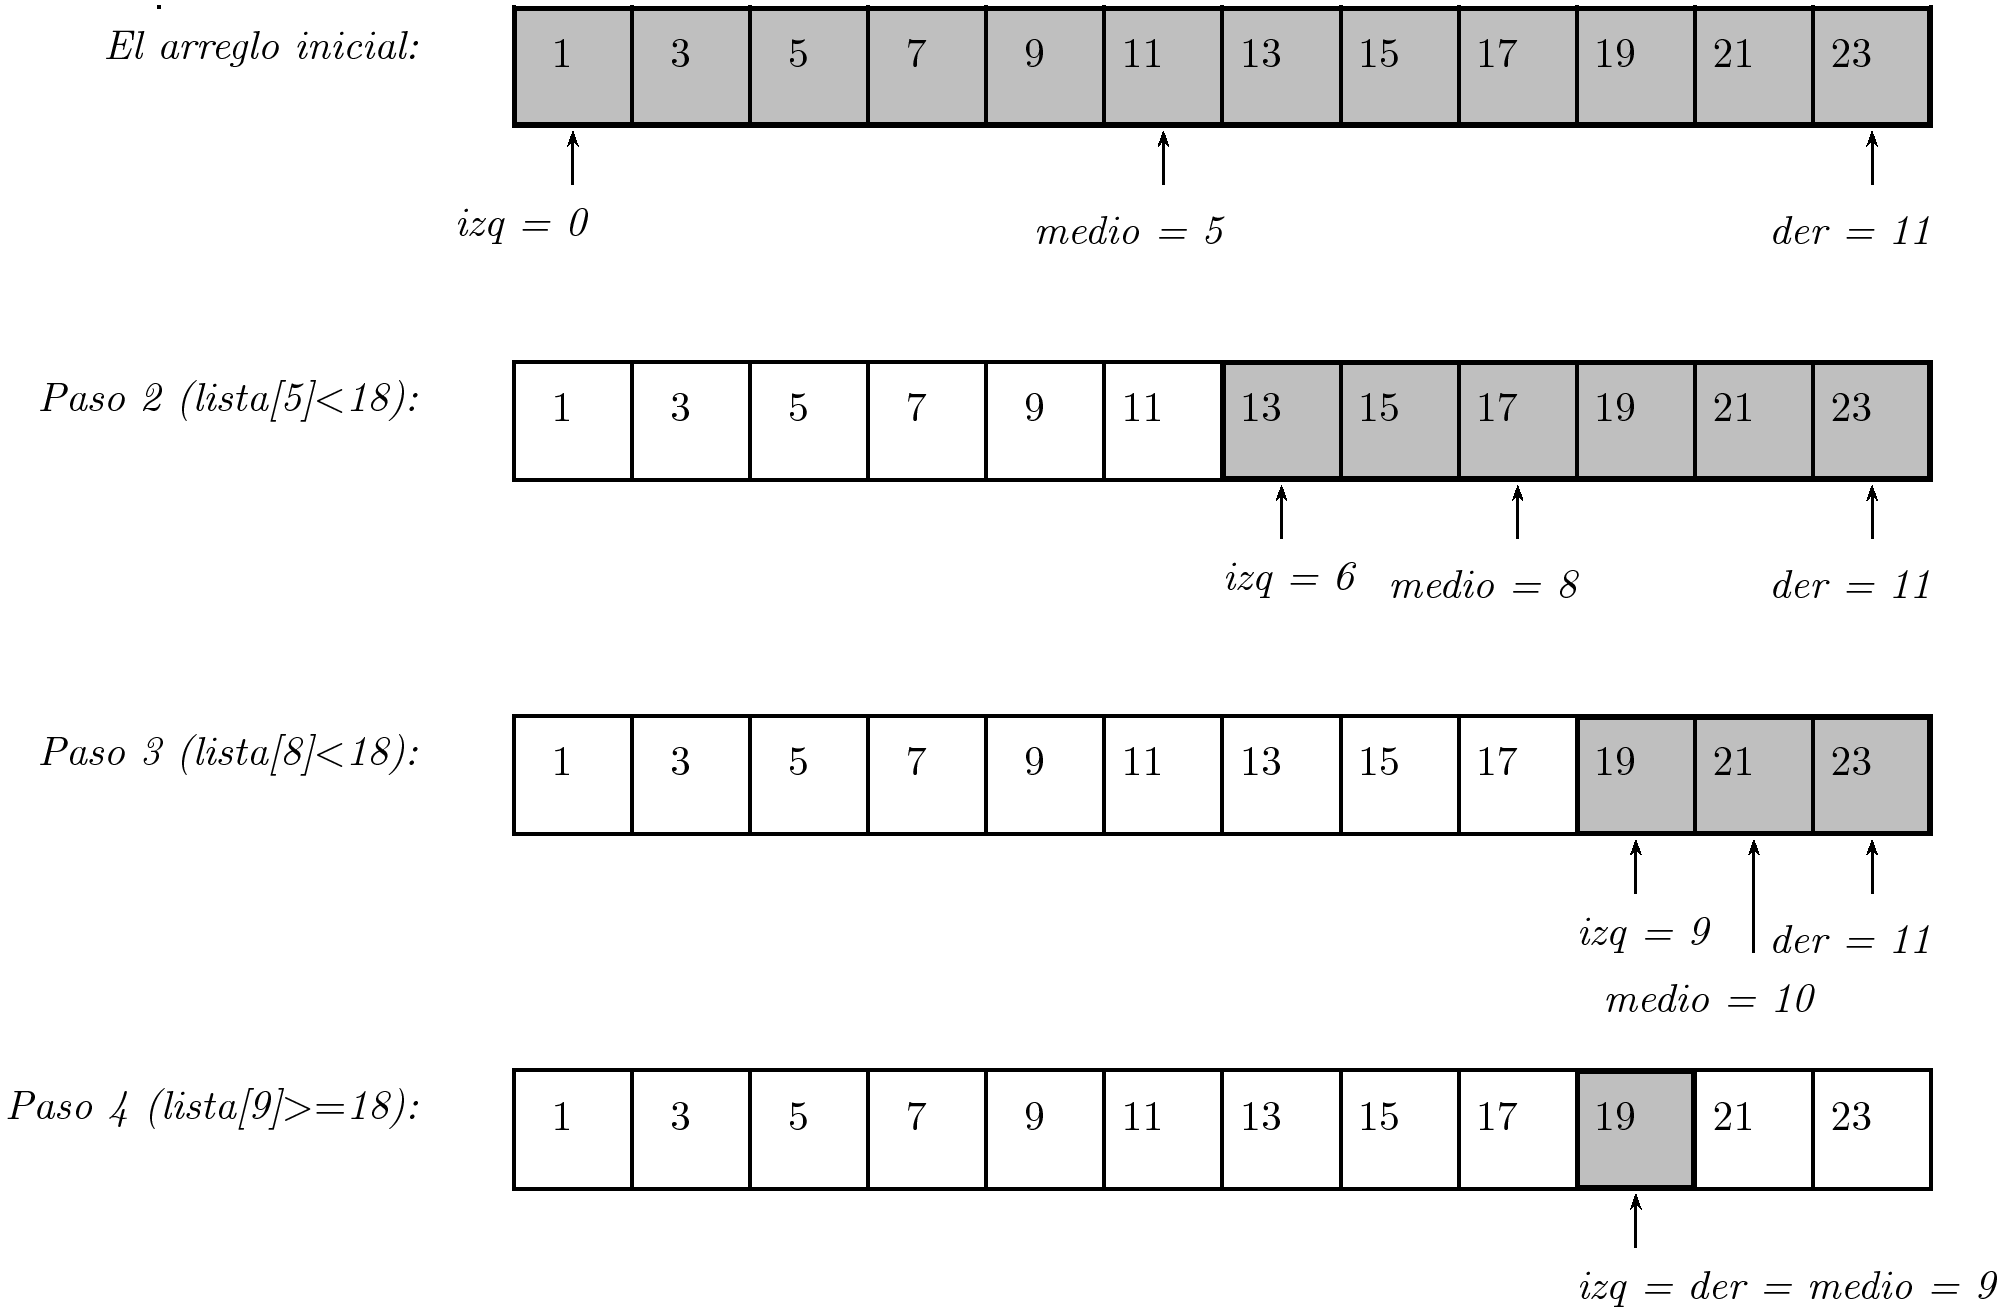
\includegraphics{graficos/uni8-seguimiento}
}

Como no se encontr� al valor buscado, devuelve $-1$.

En el C�digo \ref{busquedabinaria} mostramos una posible implementaci�n de
este algoritmo. \\

\begin{codigo}{busqueda\_binaria.py}{Funci�n de b�squeda binaria}
\label{busquedabinaria}
\lstinputlisting{src/8_busqueda/busb.py}
\end{codigo}

A continuaci�n varias ejecuciones de prueba:

\begin{verbatim}
Dame una lista ordenada ([[]] para terminar): [1, 3, 5]
�Valor buscado?: 0
DEBUG: izq: 0 der: 2 medio: 1
DEBUG: izq: 0 der: 0 medio: 0
Resultado: -1
Dame una lista ordenada ([[]] para terminar): [1, 3, 5]
�Valor buscado?: 1
DEBUG: izq: 0 der: 2 medio: 1
DEBUG: izq: 0 der: 0 medio: 0
Resultado: 0
Dame una lista ordenada ([[]] para terminar): [1, 3, 5]
�Valor buscado?: 2
DEBUG: izq: 0 der: 2 medio: 1
DEBUG: izq: 0 der: 0 medio: 0
Resultado: -1
Dame una lista ordenada ([[]] para terminar): [1, 3, 5]
�Valor buscado?: 3
DEBUG: izq: 0 der: 2 medio: 1
Resultado: 1
Dame una lista ordenada ([[]] para terminar): [1, 3, 5]
�Valor buscado?: 5
DEBUG: izq: 0 der: 2 medio: 1
DEBUG: izq: 2 der: 2 medio: 2
Resultado: 2
Dame una lista ordenada ([[]] para terminar): [1, 3, 5]
�Valor buscado?: 6
DEBUG: izq: 0 der: 2 medio: 1
DEBUG: izq: 2 der: 2 medio: 2
Resultado: -1
Dame una lista ordenada ([[]] para terminar): []
�Valor buscado?: 0
Resultado: -1
Dame una lista ordenada ([[]] para terminar): [1]
�Valor buscado?: 1
DEBUG: izq: 0 der: 0 medio: 0
Resultado: 0
Dame una lista ordenada ([[]] para terminar): [1]
�Valor buscado?: 3
DEBUG: izq: 0 der: 0 medio: 0
Resultado: -1
Dame una lista ordenada ([[]] para terminar): [[]]
\end{verbatim}

\subsection*{�Cu�ntas comparaciones hace este programa?}

Para responder esto pensemos en el peor caso, es decir, que se descartaron
varias veces partes del segmento para finalmente llegar a un segmento vac�o y
porque el valor buscado no se encontraba en la lista.

En cada paso el segmento se divide por la mitad y se desecha una de esas
mitades, y en cada paso se hace una comparaci�n con el valor buscado. Por lo
tanto, la cantidad de comparaciones que hacen con el valor buscado es
aproximadamente igual a la cantidad de pasos necesarios para llegar a un
segmento de tama�o 1.
Veamos el caso m�s sencillo para razonar, y supongamos que la longitud de la
lista es una potencia de 2, es decir \lstinline+len(lista)+$= 2^k$:

\begin{itemize}
\item Luego del primer paso, el segmento a tratar es de tama�o $2^k$.
\item Luego del segundo paso, el segmento a tratar es de tama�o $2^{k-1}$.
\item Luego del tercer paso, el segmento a tratar es de tama�o $2^{k-2}$.

$\ldots$

\item Luego del paso $k$, el segmento a tratar es de tama�o $2^{k-k}=1$.
\end{itemize}

Por lo tanto este programa hace aproximadamente $k$ comparaciones con el valor
buscado cuando \lstinline+len(lista)+$= 2^k$.
Pero si despejamos $k$ de la ecuaci�n anterior, podemos ver que este programa
realiza aproximadamente $\log_2$(\lstinline+len(lista)+) comparaciones.

Cuando \lstinline+len(lista)+ no es una potencia de 2 el razonamiento es menos
prolijo, pero tambi�n vale que este programa realiza aproximadamente
$\log_2$(\lstinline+len(lista)+) comparaciones.

Vemos entonces que si \lstinline!lista! es una lista ordenada, la b�squeda binaria es
\underline{much�simo} m�s eficiente que la b�squeda lineal (por ejemplo, dado
que $2^{20}$ es aproximadamente 1.000.000, si \lstinline!lista! tiene 1.000.000 de
elementos, la b�squeda lineal sobre \lstinline+lista+ ser� proporcional a 1.000.000, y
en promedio har� unas 500.000 comparaciones, mientras que la b�squeda binaria
har� como m�ximo 20 comparaciones).

\section{Resumen}

\begin{itemize}

\item La {\bf b�squeda} de un elemento en una secuencia es un
algoritmo b�sico pero importante. El problema que intenta resolver puede
plantearse de la siguiente manera: Dada una secuencia de valores y un
valor, devolver el �ndice del valor en la secuencia, si se encuentra, de no
encontrarse el valor en la secuencia se�alizarlo apropiadamente.

\item Una de las formas de resolver el problema es mediante la {\bf
b�squeda lineal}, que consiste en ir revisando uno a uno los elementos de
la secuencia y compar�ndolos con el elemento a buscar.  Este algoritmo no
requiere que la secuencia se encuentre ordenada.

\item Cuando la secuencia sobre la que se quiere buscar est� ordenada, se
puede utilizar el algoritmo de {\bf b�squeda binaria}.  Al estar ordenada
la secuencia, se puede desacartar en cada paso la mitad de los elementos,
quedando entonces con una eficiencia algor�tmica relativa al
$log($\lstinline!len(secuencia)!$)$. Este algoritmo s�lo tiene sentido
utilizarlo sobre una secuencia ordenada.

\item El an�lisis del comportamiento de un algoritmo puede ser muy enga�oso
si se tiene en cuenta el mejor caso, por eso suele ser mucho m�s
ilustrativo tener en cuenta el {\bf peor caso}.  En algunos casos
particulares podr� ser �til tener en cuenta, adem�s, el {\bf caso
promedio}.

\end{itemize}


% Copyright (C) 2009 Marcos Medrano <marcosmedrano0@gmail.com>
% Copyright (C) 2009-2010 Margarita Manterola <margamanterola@gmail.com>

% Esta obra est� licenciada de forma dual, bajo las licencias Creative
% Commons:
%  * Atribuci�n-Compartir Obras Derivadas Igual 2.5 Argentina
%    http://creativecommons.org/licenses/by-sa/2.5/ar/
%  * Atribuci�n-Compartir Obras Derivadas Igual 3.0 Unported
%    http://creativecommons.org/licenses/by-sa/3.0/deed.es_AR.
%
% A su criterio, puede utilizar una u otra licencia, o las dos.
% Para ver una copia de las licencias, puede visitar los sitios
% mencionados, o enviar una carta a Creative Commons,
% 171 Second Street, Suite 300, San Francisco, California, 94105, USA.

\chapter{Diccionarios}

En esta unidad analizaremos otro tipo de dato importante: los diccionarios.
Su importancia, radica no s�lo en las grandes posibilidades que presentan
como estructuras para almacenar informaci�n, sino tambi�n en que, en
Python, son utilizados por el propio lenguaje para realizar diversas
operaciones y para almacenar informaci�n de otras estructuras.

\section{Qu� es un diccionario}

Seg�n Wikipedia, ``[u]n diccionario es una obra de consulta de
palabras y/o t�rminos que se encuentran generalmente ordenados
alfab�ticamente. De dicha compilaci�n de palabras o t�rminos se
proporciona su significado, etimolog�a, ortograf�a y, en el caso
de ciertas lenguas fija su pronunciaci�n y separaci�n sil�bica.''


Al igual que los diccionarios a los que se refiere Wikipedia, y
que usamos habitualmente en la vida diaria, los diccionarios de
Python son una lista de consulta de t�rminos de los cuales se
proporcionan valores asociados. A diferencia de los diccionarios a
los que se refiere Wikipedia, los diccionarios de Python no est�n
ordenados.


En Python, un diccionario es una colecci�n no-ordenada de valores
que son accedidos a traves de una clave.  Es decir, en lugar de
acceder a la informaci�n mediante el �ndice num�rico, como es el
caso de las listas y tuplas, es posible acceder a los valores a
trav�s de sus claves, que pueden ser de diversos tipo.

%En algunos casos usaremos key,value (o
%simplemente k,v) para referirnos a los conceptos de clave, valor. *

Las claves son �nicas dentro de un diccionario, es decir que no puede haber
un diccionario que tenga dos veces la misma clave, si se asigna un valor a
una clave ya existente, se reemplaza el valor anterior.

No hay una forma directa de acceder a una clave a trav�s de su valor, y
nada impide que un mismo valor se encuentre asignado a distintas claves

La informacion almacenada en los diccionarios, no tiene un orden
particular.  Ni por clave ni por valor, ni tampoco por el orden en
que han sido agregados al diccionario.

Cualquier variable de tipo inmutable, puede ser clave de un diccionario:
cadenas, enteros, tuplas (con valores inmutables en sus miembros), etc.  No hay
restricciones para los valores que el diccionario puede contener, cualquier
tipo puede ser el valor: listas, cadenas, tuplas, otros diccionarios, objetos,
etc.

\begin{sabias_que}
En otros lenguajes, a los diccionarios se los llama {\it arreglos
asociativos}, {\it matrices asociativas}, o tambi�n {\it tablas de hash}.
\end{sabias_que}

\section{Utilizando diccionarios en Python}

De la misma forma que con listas, es posible definir un diccionario
directamente con los miembros que va a contener, o bien inicializar el
diccionario vac�o y luego agregar los valores de a uno o de a muchos.

Para definirlo junto con los miembros que va a contener, se encierra el
listado de valores entre llaves, las parejas de clave y valor se separan
con comas, y la clave y el valor se separan con ':'.

\begin{codigo-python-sn}
punto = {'x': 2, 'y': 1, 'z': 4}
\end{codigo-python-sn}

Para declararlo vac�o y luego ingresar los valores, se lo declara como un
par de llaves sin nada en medio, y luego se asignan valores directamente a
los �ndices.

\begin{codigo-python-sn}
materias = {}
materias["lunes"] = [6103, 7540]
materias["martes"] = [6201]
materias["mi�rcoles"] = [6103, 7540]
materias["jueves"] = []
materias["viernes"] = [6201]
\end{codigo-python-sn}

Para acceder al valor asociado a una determinada clave, se lo hace
de la misma forma que con las listas, pero utilizando la clave
elegida en lugar del �ndice.

\begin{codigo-python-sn}
print materias["lunes"]
\end{codigo-python-sn}

Sin embargo, esto falla si se provee una clave que no est� en el diccionario.
Es posible, por otro lado, utilizar la funci�n \lstinline{get}, que devuelve el
valor \lstinline{None} si la clave no est� en el diccionario, o un valor por
omisi�n que se establece opcionalmente.

\begin{codigo-python-sn}
>>> print materias["domingo"]
Traceback (most recent call last):
  File "<stdin>", line 1, in <module>
KeyError: 'domingo'
>>> print materias.get("domingo")
None
>>> print materias.get("domingo", [])
[]
\end{codigo-python-sn}

Existen diversas formas de recorrer un diccionario.  Es posible recorrer
sus claves y usar esas claves para acceder a los valores.

\begin{codigo-python-sn}
for dia in materias:
    print dia, ":", materias[dia]
\end{codigo-python-sn}

Es posible, tambi�n, obtener los valores como tuplas donde el primer
elemento es la clave y el segundo el valor.

\begin{codigo-python-sn}
for dia, codigos in materias.items():
    print dia, ":", codigos
\end{codigo-python-sn}

Para verificar si una clave se encuentra en el diccionario, es posible
utilizar la funci�n \lstinline{has_key} o la palabra reservada
\lstinline{in}.

\begin{codigo-python-sn}
d = {'x': 12, 'y': 7}
if d.has_key('x'):
    print d['x']   # Imprime 12
if d.has_key('z'): 
    print d['z']   # No se ejecuta
if 'y' in d:
    print d['y']   # Imprime 7
\end{codigo-python-sn}

M�s all� de la creaci�n y el acceso, hay muchas otras operaciones que se
pueden realizar sobre los diccionarios, para poder manipular la informaci�n
seg�n sean nuestras necesidades, algunos de estos m�todos pueden verse en
la referencia al final de la unidad.

\begin{sabias_que}
El algoritmo que usa Python internamente para buscar un elemento en un
diccionario es muy distinto que el que utiliza para buscar en listas.

Para buscar en las listas, se utiliza un algoritmos de comparaci�n que
tarda cada vez m�s a medida que la lista se hace m�s larga.  En cambio,
para buscar en diccionarios se utiliza un algoritmo llamado {\it hash},
que se basa en realizar un c�lculo num�rico sobre la clave del elemento, 
y tiene una propiedad muy interesante: sin importar cu�ntos elementos
tenga el diccionario, el tiempo de b�squeda es siempre aproximadamente
igual.

Este algoritmo de {\it hash} es tambi�n la raz�n por la cual las claves de
los diccionarios deben ser inmutables, ya que la operaci�n hecha sobre las
claves debe dar siempre el mismo resultado, y si se utilizara una variable
mutable esto no ser�a posible.
\end{sabias_que}

No es posible obtener porciones de un diccionario usando \lstinline![:]!,
ya que al no tener un orden determinado para los elementos, no ser�a
posible tomarlos en orden.

\section{Algunos usos de diccionarios}

Los diccionarios son una herramienta muy vers�til.  Se puede utilizar un
diccionario, por ejemplo, para contar cu�ntas apariciones de cada palabra
hay en un texto, o cu�ntas apariciones de cada letra.  

Es posible utilizar un diccionario, tambi�n, para tener una agenda donde la
clave es el nombre de la persona, y el valor es una lista con los datos
correspondientes a esa persona.

Tambi�n podr�a utilizarse un diccionario para mantener los datos de los
alumnos inscriptos en una materia.  Siendo la clave el n�mero de padr�n, y
el valor una lista con todas las notas asociadas a ese alumno.

En general, los diccionarios sirven para crear bases de datos muy simples,
en las que la clave es el identificador del elemento, y el valor son todos
los datos del elemento a considerar.

Otro posible uso de un diccionario ser�a utilizarlo para realizar
traducciones, donde la clave ser�a la palabra en el idioma original y el
valor la palabra en el idioma al que se quiere traducir.  Sin embargo esta
aplicaci�n es poco destacable, ya que esta forma de traducir es muy mala.

\section{Resumen}

\begin{itemize}
\item Los diccionarios (llamados {\it arreglos asociativos} o {\it tablas
de hash} en otros lenguajes), son una estructura de datos muy poderosa, que permite
asociar un valor a una clave.
\item Las claves deben ser de tipo inmutable, los valores
pueden ser de cualquier tipo.
\item Los diccionarios no est�n ordenados.  Si bien se los puede recorrer,
el orden en el que se tomar�n los elementos no est� determinado.
\end{itemize}

\begin{referencia_python}

\begin{sintaxis}{\lstinline!\{clave1:valor1, clave2:valor2\}!}
Se crea un nuevo diccionario con los valores asociados a las claves.  Si no
se ingresa ninguna pareja de clave y valor, se crea un diccionario vac�o.
\end{sintaxis}

\begin{sintaxis}{\lstinline{diccionario[clave]}}
Accede al valor asociado con \lstinline!clave! en el diccionario.
\end{sintaxis}

\begin{sintaxis}{\lstinline{diccionario.has_key(clave)}}
Indica si un diccionario tiene o no una determinada clave.
Es posible obtener el mismo resultado utilizando:
\lstinline{if clave in diccionario:}.
\end{sintaxis}

\begin{sintaxis}{\lstinline{diccionario.get(clave[, valor_predeterminado])}}
Devuelve el valor asociado a la clave.  A diferencia del acceso directo
utilizando \lstinline{[clave]}, en el caso en que el valor no se
encuentre, no da un error, sino que devuelve el valor predeterminado o
\lstinline{None} en el caso de que no se haya establecido.
\end{sintaxis}

\begin{sintaxis}{\lstinline{for clave in diccionario:}}
Esta estructura permite recorrer una a una todas las claves almacenadas en
el diccionario.
\end{sintaxis}

\begin{sintaxis}{\lstinline{diccionario.keys()}}
Devuelve una lista desordenada, con todas las claves que se hayan ingresado
al diccionario
\end{sintaxis}

\begin{sintaxis}{\lstinline{diccionario.values()}}
Devuelve una lista desordenada, con todos los valores que se hayan
ingresado al diccionario.
\end{sintaxis}

\begin{sintaxis}{\lstinline{diccionario.items()}}
Devuelve una lista desordenada con tuplas de dos elementos, en las que el
primer elemento es la clave y el segundo el valor.
\end{sintaxis}

\begin{sintaxis}{\lstinline{diccionario.pop(clave)}}
Devuelve el valor asociado a la clave, y elimina la clave y el valor
asociado del diccionario.
\end{sintaxis}

\begin{sintaxis}{\lstinline{diccionario.popitem()}}
Devuelve un elemento al azar del diccionario, represent�ndolo como una
tupla \lstinline{(clave, valor)} y elimina esta pareja del diccionario.
\end{sintaxis}

\begin{sintaxis}{\lstinline{diccionario.clear()}}
Elimina todos los elementos del diccionario
\end{sintaxis}

% Lo saco porque se va de la hoja, y aporta poco
%\begin{sintaxis}{\lstinline{diccionario.update(otro_diccionario)}}
%
%Actualiza los valores del diccionario con los recibidos por par�metro.  Si
%una clave est� en ambos, se modifica el valor asociado en
%\lstinline{diccionario}, para que tenga el mismo valor que en
%\lstinline{otro_diccionario}.  Si una clave no est� en
%\lstinline{diccionario}, se agrega con el valor que tenga en
%\lstinline{otro_diccionario}.
%
%\end{sintaxis}

\end{referencia_python}


\newpage
\section{Ejercicios}

\ejercicio{
Escribir una funci�n que reciba una lista de tuplas, y que devuelva
un diccionario en donde las claves sean los primeros elementos de las
tuplas, y los valores una lista con los segundos.}

Por ejemplo: 
\begin{lstlisting}[numbers=none]
l = [ ('Hola', 'don Pepito'), ('Hola', 'don Jose'), ('Buenos', 'd�as') ]
print tuplas_a_diccionario(l)
\end{lstlisting}

Deber� mostrar: \lstinline!{ 'Hola': ['don Pepito', 'don Jose'], 'Buenos': ['d�as'] }!

\ejercicio{\bf Diccionarios usados para contar.}
\begin{partes}
  \item Escribir una funci�n que reciba una cadena y devuelva un diccionario con
la cantidad de apariciones de cada palabra en la cadena.  Por ejemplo, si
recibe "Qu� lindo d�a que hace hoy" debe devolver: { 'que': 2, 'lindo': 1,
'd�a': 1, 'hace': 1, 'hoy': 1}
  \item Escribir una funci�n que cuente la cantidad de apariciones de cada
caracter en una cadena de texto, y los devuelva en un diccionario.
  \item Escribir una funci�n que reciba una cantidad de iteraciones de una tirada
de 2 dados a realizar y devuelva la cantidad de veces que se observa cada valor
de la suma de los dos dados. \\
{\bf Nota}: utilizar el m�dulo \verb!random! para obtener tiradas aleatorias.
\end{partes}

\ejercicio{{\bf Continuaci�n de la agenda}. \\
Escribir un programa que vaya solicitando al usuario que ingrese nombres.}
\begin{partes}
  \item Si el nombre se encuentra en la agenda ({\it implementada con un
diccionario}), debe mostrar el tel�fono y, opcionalmente, permitir
modificarlo si no es correcto.
  \item Si el nombre no se encuentra, debe permitir ingresar el tel�fono
correspondiente.
\end{partes}
El usuario puede utilizar la cadena "*", para salir del programa.

\ejercicio{
Escribir una funci�n que reciba un texto y para cada caracter presente en el
texto devuelva la cadena m�s larga en la que se encuentra ese caracter.
}


% Copyright (C) 2009-2010 Maximiliano Curia <maxy@gnuservers.com.ar>,
%               Margarita Manterola <margamanterola@gmail.com>

% Esta obra est� licenciada de forma dual, bajo las licencias Creative
% Commons:
%  * Atribuci�n-Compartir Obras Derivadas Igual 2.5 Argentina
%    http://creativecommons.org/licenses/by-sa/2.5/ar/
%  * Atribuci�n-Compartir Obras Derivadas Igual 3.0 Unported
%    http://creativecommons.org/licenses/by-sa/3.0/deed.es_AR.
%
% A su criterio, puede utilizar una u otra licencia, o las dos.
% Para ver una copia de las licencias, puede visitar los sitios
% mencionados, o enviar una carta a Creative Commons,
% 171 Second Street, Suite 300, San Francisco, California, 94105, USA.

\chapter{Contratos y Mutabilidad}

En esta unidad se le dar� cierta formalizaci�n a algunos temas que se hab�an
visto informalmente, como por ejemplo, la documentaci�n de las funciones. 

Se formalizar�n las condiciones que debe cumplir un algoritmo, al comenzar, en
su transcurso, y al terminar, y algunas t�cnicas para tener en cuenta estas
condiciones.

Tambi�n se ver� una forma de modelizar el espacio donde \textit{viven} las
variables.

\section{Pre y Postcondiciones}

Cuando hablamos de \textit{contratos} o \textit{programaci�n por
contratos}, nos referimos a la necesidad de estipular tanto lo que necesita
como lo que devuelve nuestro c�digo. 

Las condiciones que deben estar dadas para que el c�digo funcione las llamamos
\emph{precondiciones} y las condiciones sobre el estado en que quedan las
variables y �l o los valores de retorno, las llamamos \emph{postcondiciones}.

En definitiva, este concepto es similar al ya mencionado con respecto a la
documentaci�n de funciones, es decir que se debe \emph{documentar c�mo deben
ser los par�metros recibidos, c�mo va a ser lo que se devuelve, y qu�
sucede con los par�metros en caso de ser modificados}.

Esta estipulaci�n es mayormente para que la utilicen otros programadores,
por lo que es particularmente �til cuando se encuentra dentro de la
documentaci�n. En ciertos casos, adem�s, puede quererse que el programa
revise si las condiciones realmente se cumplen y de no ser as�, act�e en
consecuencia.

Existen herramientas en algunos lenguajes de programaci�n que facilitan estas
acciones, en el caso de Python, es posible utilizar la instrucci�n
\lstinline!assert!.
 
\subsection{Precondiciones}

Las precondiciones son las condiciones que deben cumplir los par�metros que
una funci�n recibe, para que esta se comporte correctamente.

Por ejemplo, en una funci�n divisi�n las precondiciones son que los par�metros
son n�meros, y que el divisor sea distinto de 0. Tener una precondici�n
permite asumir desde el c�digo que no es necesario lidiar con los casos en que
las precondiciones no se cumplen.

\subsection{Postcondiciones}

Las postcodiciones son las condiciones que cumplir� el valor de retorno, y
los par�metros recibidos, en caso de que hayan sido alterados, 
siempre que se hayan cumplido las precondiciones 

En el ejemplo anterior, la funci�n divisi�n con las precondiciones asignadas,
puede asegurar que devolver� un n�mero correspondiente al cociente solicitado.

\subsection{Aseveraciones}

Tanto las precondiciones como las postcondiciones son \textit{aseveraciones}
(en ingl�s \textit{assert}). Es decir, afirmaciones realizadas en un momento
particular de la ejecuci�n sobre el estado computacional. Si llegaran a ser
falsas significar�a que hay alg�n error en el dise�o o utilizaci�n del algoritmo.

Para comprobar estas afirmaciones desde el c�digo en algunos casos podemos
utilizar la instrucci�n \lstinline!assert!, est� instrucci�n recibe una
condici�n a verificar y, opcionalmente, un mensaje de error que devolver� en
caso que la condici�n no se cumpla.

\begin{codigo-python-sn}
>>> n=0
>>> assert n!=0, "El divisor no puede ser 0"
Traceback (most recent call last):
  File "<stdin>", line 1, in <module>
AssertionError: El divisor no puede ser 0
\end{codigo-python-sn}

\begin{atencion}
Es importante tener en cuenta que \lstinline!assert! est� pensado para ser
usado en la etapa de desarrollo. Un programa terminado nunca deber�a dejar
de funcionar por este tipo de errores.
\end{atencion}

\subsection{Ejemplos}

Usando los ejemplos anteriores, la funci�n \lstinline!division! nos
quedar�a de la siguiente forma:

\begin{codigo-python-sn}
def division(dividendo, divisor):
    """ Calculo de la divisi�n

    Pre: Recibe dos n�meros, divisor debe ser distinto de 0.
    Post: Devuelve un n�mero real, con el cociente de ambos.	
    """
    assert divisor != 0, "El divisor no puede ser 0"
    return dividendo  / ( divisor * 1.0 )
\end{codigo-python-sn}

Otro ejemplo, tal vez m�s interesante, puede ser una funci�n que implemente
una sumatoria ($\sum_{i=inicial}^{final} f(i)$).  En este caso hay que
analizar cu�les van a ser los par�metros que recibir� la funci�n, y las
precondiciones que estos par�metros deber�n cumplir.

La funci�n sumatoria a escribir, necesita de un valor inicial, un valor
final, y una funci�n a la cual llamar en cada paso. Es decir que recibe
tres par�metros.

\begin{codigo-python-sn}
def sumatoria(inicial, final, f):
\end{codigo-python-sn}

Tanto \lstinline!inicial! como \lstinline!final! deben ser n�meros enteros,
y dependiendo de la implementaci�n a realizar o de la especificaci�n
previa, puede ser necesario que \lstinline!final! deba ser mayor o igual a
\lstinline!inicial!.

Con respecto a \lstinline!f!, se trata de una funci�n que ser� llamada con
un par�metro en cada paso y se requiere poder sumar el resultado, por lo
que debe ser una funci�n que reciba un n�mero y devuelva un n�mero.

La declaraci�n de la funci�n queda, entonces, de la siguiente manera.

\begin{codigo-python-sn}
def sumatoria(inicial, final, f):
    """Calcula la sumatoria desde i=inicial hasta final de f(i)

    Pre: inicial y final son n�meros enteros, f es una funci�n que 
         recibe un entero y devuelve un n�mero.
    Post: Se devuelve el valor de la sumatoria de aplicar f a cada
          n�mero comprendido entre inicial y final.
	"""
\end{codigo-python-sn}

\begin{ejercicio}
Realizar la implementaci�n correspondiente a la funci�n \lstinline!sumatoria!.
\end{ejercicio}

En definitiva, la documentaci�n de pre y postcondiciones dentro de la documentaci�n
de las funciones es una forma de especificar claramente el comportamiento del
c�digo de forma que quienes lo vayan a utilizar no requieran conocer c�mo est�
implementado para poder aprovecharlo.

Esto es �til incluso en los casos en los que el programador de las funciones
es el mismo que el que las va a utilizar, ya que permite separar
responsabilidades. Las pre y postcondiciones son, en efecto, un
\textit{contrato} entre el c�digo invocante y el invocado.

\section{Invariantes de ciclo}

% TODO: conseguir frase, la vida es siempre igual, siempre est� cambiando.
%\begin{quote}
%``Dadme un punto de apoyo y mover� el mundo�� Arqu�medes
%\end{quote}

Los invariantes se refieren a estados o situaciones que no cambian dentro
de un contexto o porci�n de c�digo.  Hay invariantes de ciclo, que son los
que veremos a continuaci�n, e invariantes de estado, que se ver�n m�s
adelante.

El invariante de ciclo permite conocer c�mo llegar desde las precondiciones
hasta las postcondiciones. El invariante de ciclo es, entonces, una
aseveraci�n que debe ser verdadera al comienzo de cada iteraci�n.

Por ejemplo, si el problema es ir desde el punto A al punto B, las
precondiciones dicen que estamos parados en A y las postcondiciones que
estamos parados en B, un invariante podr�a ser ``estamos en alg�n punto entre
A y B, en el punto m�s cercano a B que estuvimos hasta ahora.''.

M�s espec�ficamente, si analizamos el ciclo para buscar el m�ximo en una lista
desordenada, la precondici�n es que la lista contiene elementos que son
comparables y la postcondici�n es que se devuelve el elemento m�ximo de la
lista.

\begin{codigo-python}
def maximo(lista):
    "Devuelve el elemento m�ximo de la lista o None si est� vac�a."
    if not len(lista):
        return None
    max_elem = lista[0]
    for elemento in lista:
        if elemento > max_elem:
            max_elem = elemento
    return max_elem
\end{codigo-python}

En este caso, el invariante del ciclo es que \lstinline!max_elem! contiene el
valor m�ximo de la porci�n de lista analizada. \\

Los invariantes son de gran importancia al momento de demostrar que un
algoritmo funciona, pero a�n cuando no hagamos una demostraci�n formal es muy
�til tener los invariantes a la vista, ya que de esta forma es m�s f�cil
entender c�mo funciona un algoritmo y encontrar posibles errores.

Los invariantes, adem�s, son �tiles a la hora de determinar las condiciones
iniciales de un algoritmo, ya que tambi�n deben cumplirse para ese caso.  Por
ejemplo, consideremos el algoritmo para obtener la potencia \lstinline!n! de
un n�mero.  

\begin{codigo-python}
def potencia(b, n):
    "Devuelve la potencia n del n�mero b, con n entero mayor que 0."
    p = 1
    for i in range(n):
        p *= b
    return p
\end{codigo-python}

En este caso, el invariante del ciclo es que la variable \lstinline!p!
contiene el valor de la potencia correspondiente a esa iteraci�n. Teniendo en
cuenta esta condici�n, es f�cil ver que \lstinline!p! debe comenzar el ciclo
con un valor de 1, ya que ese es el valor correspondiente a $p^0$.

De la misma manera, si la operaci�n que se quiere realizar es sumar todos los
elementos de una lista, el invariante ser� que una variable \lstinline!suma!
contenga la suma de todos los elementos ya recorridos, por lo que es claro que
este invariante debe ser 0 cuando a�n no se haya recorrido ning�n elemento.

\begin{codigo-python}
def suma(lista):
    "Devuelve la suma de todos los elementos de la lista."
    suma = 0
    for elemento in lista:
        suma += elemento
    return suma
\end{codigo-python}

% TODO
% \subsection{Invariantes como medida de cu�nto falta}

%Dependiendo del problema y las herramientas con las que contemos algunos
%invariantes se pueden medir retomando el ejemplo de ir de A a B, uno podr�a
%medir la distancia hasta B para esta, pero si para medir la distancia hay que ir hasta B
%y volver deja de tener sentido. O al estar buscando el m�nimo en una
%secuencia, c�mo hago para comprobar que paso a paso tengo el m�nimo de la
%secuencia que ya recorr� sin usar

\subsection{Comprobaci�n de invariantes desde el c�digo}

Cuando la comprobaci�n necesaria para saber si seguimos ``en camino'' es simple,
se la puede tener directamente dentro del c�digo.  Evitando seguir avanzando
con el algoritmo si se produjo un error cr�tico.

Por ejemplo, en una b�squeda binaria, el elemento a buscar debe ser mayor que
el elemento inicial y menor que el elemento final, de no ser as�, no tiene sentido
continuar con la b�squeda.  Es posible, entonces, agregar una instrucci�n
que compruebe esta condici�n y de no ser cierta realice alguna acci�n para
indicar el error, por ejemplo, utilizando la instrucci�n \lstinline!assert!,
vista anteriormente. 

\section{Mutabilidad e Inmutabilidad}

Hasta ahora cada vez que estudiamos un tipo de variables indicamos si son
mutables o inmutables.

Cuando una variable es de un tipo inmutable, como por ejemplo una cadena, es
posible asignar un nuevo valor a esa variable, pero no es posible modificar su
contenido.

\begin{codigo-python-sn}
>>> a="ejemplo"
>>> a="otro"
>>> a[2]="c"
Traceback (most recent call last):
  File "<stdin>", line 1, in <module>
TypeError: 'str' object does not support item assignment
\end{codigo-python-sn}

Esto se debe a que cuando se realiza una nueva asignaci�n, no se modifica la
cadena en s�, sino que la variable \lstinline!a! pasa a \emph{apuntar} a otra cadena.
En cambio, no es posible asignar un nuevo caracter en una posici�n, ya que
esto implicar�a modificar la cadena inmutable.

En el caso de los par�metros mutables, la asignaci�n tiene el mismo
comportamiento, es decir que las variables pasan a apuntar a un nuevo valor.

\begin{codigo-python-sn}
>>> lista1 = [10, 20, 30]
>>> lista2 = lista1
>>> lista1 = [3, 5, 7]
>>> lista1
[3, 5, 7]
>>> lista2
[10, 20, 30]
\end{codigo-python-sn}

Algo importante a tener en cuenta en el caso de las variables de tipo
mutable es que si hay dos o m�s variables que \textit{apuntan} a un mismo
dato, y este dato se modifica, el cambio se ve reflejado en ambas variables.

\begin{codigo-python-sn}
>>> lista1=[1, 2, 3]
>>> lista2 = lista1
>>> lista2[1] = 5
>>> lista1
[1, 5, 3]
\end{codigo-python-sn}

\begin{sabias_que}
En otros lenguajes, como C o C++, existe un tipo de variable especial
llamado {\it puntero}, que se comporta como una referencia a una variable,
como es el caso de las variables mutables del ejemplo anterior.

En Python no hay punteros como los de C o C++, pero todas las variables son
referencias a una porci�n de memoria, de modo que cuando se asigna una
variable a otra, lo que se est� asignando es la porci�n de memoria a la que
refieren.  Si esa porci�n de memoria cambia, el cambio se puede ver en
todas las variables que apuntan a esa porci�n.
\end{sabias_que}

% TODO: describir en m�s detalle el modelo de referencia de python ?

\subsection{Par�metros mutables e inmutables}

Las funciones reciben par�metros que pueden ser mutables o inmutables.

Si dentro del cuerpo de la funci�n se modifica uno de estos par�metros para
que \textbf{apunte} a otro valor, este cambio no se ver� reflejado fuera de la
funci�n.  Si, en cambio, se modifica el \textbf{contenido} de alguno de los
par�metros mutables, este cambio \textbf{s�} se ver� reflejado fuera de la
funci�n.

A continuaci�n un ejemplo en el cual se asigna la variable recibida, a un
nuevo valor.  Esa asignaci�n s�lo tiene efecto dentro de la funci�n.

\begin{codigo-python-sn}
>>> def no_cambia_lista(lista):
...     lista = range(len(lista))
...     print lista
...
>>> lista = [10, 20, 30, 40]
>>> no_cambia_lista(lista)
[0, 1, 2, 3]
>>> lista
[10, 20, 30, 40]
\end{codigo-python-sn}

A continuaci�n un ejemplo en el cual se modifica la variable recibida. En este
caso, los cambios realizados tienen efecto tanto dentro como fuera de la
funci�n.

\begin{codigo-python-sn}
>>> def cambia_lista(lista):
...     for i in range(len(lista)):
...             lista[i] = lista[i]**3
...
>>> lista = [1, 2, 3, 4]
>>> cambia_lista(lista)
>>> lista
[1, 8, 27, 64]
\end{codigo-python-sn}

\begin{atencion}
En general, se espera que una funci�n que recibe par�metros mutables, no los
modifique, ya que si se los modifica se podr�a perder informaci�n valiosa.

En el caso en que por una decisi�n de dise�o o especificaci�n se modifiquen
los par�metros recibidos, esto debe estar claramente documentado, dentro de
las postcondiciones.
\end{atencion}

\section{Resumen}

\begin{itemize}
\item Las \textbf{precondiciones} son las condiciones que deben cumplir los
par�metros recibidos por una funci�n.
\item Las \textbf{postcondiciones} son las condiciones cumplidads por los
resultados que la funci�n devuelve y por los par�metros recibidos, siempre
que las precondiciones hayan sido v�lidas.
\item Los \textbf{invariantes de ciclo} son las condiciones que deben
cumplirse al comienzo de cada iteraci�n de un ciclo.
\item En el caso en que estas \textbf{aseveraciones} no sean verdaderas, se
deber� a un error en el dise�o o utilizaci�n del c�digo.
\item En general una funci�n no debe modificar el contenido de sus par�metros,
a�n cuando esto sea posible, a menos que sea la funcionalidad expl�cita de esa
funci�n.
\end{itemize}

\begin{referencia_python}

\begin{sintaxis}{\lstinline!assert condicion[,mensaje]!}
Verifica si la condici�n es verdadera.  En caso contrario, levanta una
excepci�n con el mensaje recibido por par�metro.
\end{sintaxis}

\end{referencia_python}

\section{Ap�ndice - Acertijo MU}

El acertijo MU\footnote{
\url{http://en.wikipedia.org/wiki/Invariant\_(computer\_science)}} es un buen
ejemplo de un problema l�gico donde es �til determinar el invariante.  El
acertijo consiste en buscar si es posible convertir MI a MU, utilizando las
siguientes operaciones.

\begin{enumerate}
\item Si una cadena termina con una I, se le puede agregar una U (xI -> xIU)
\item Cualquier cadena luego de una M puede ser totalmente duplicada (Mx ->
Mxx)
\item Donde haya tres Is consecutivas (III) se las puede reemplazar por una U
(xIIIy -> xUy)
\item Dos Us consecutivas, pueden ser eliminadas (xUUy -> xy)
\end{enumerate}

Para resolver este problema, es posible pasar horas aplicando estas reglas
a distintas cadenas.  Sin embargo, puede ser m�s f�cil encontrar una
afirmaci�n que sea invariante para todas las reglas y que muestre si es o
no posible llegar a obtener MU.

Al analizar las reglas, la forma de deshacerse de las Is es conseguir tener
tres Is consecutivas en la cadena.  La �nica forma de deshacerse de todas las
Is es que haya un cantidad de Is consecutivas m�ltiplo de tres.

Es por esto que es interesante considerar la siguiente afirmaci�n como
invariante: el n�mero de Is en la cadena no es m�ltiplo de tres.

Para que esta afirmaci�n sea invariante al acertijo, para
cada una de las reglas se debe cumplir que: si el invariante era verdadero
antes de aplicar la regla, seguir� siendo verdadero luego de aplicarla.

Para ver si esto es cierto o no, es necesario considerar la aplicaci�n del
invariante para cada una de las reglas.

\begin{enumerate}
\item Se agrega una U, la cantidad de Is no var�a, por lo cual se mantiene el
invariante.
\item Se duplica toda la cadena luego de la M, siendo $n$ la cantidad de
Is antes de la duplicaci�n, si $n$ no es m�ltiplo de 3, $2n$ tampoco lo ser�.
\item Se reemplazan tres Is por una U.  Al igual que antes, siendo $n$ la
cantidad de Is antes del reemplazo, si $n$ no es m�ltiplo de 3, $n-3$ tampoco
lo ser�.
\item Se eliminan Us, la cantidad de Is no var�a, por lo cual se mantiene el
invariante.
\end{enumerate}

Todo esto indica claramente que el invariante se mantiene para cada una de las
posibles transformaciones.  Esto significa que sea cual fuere la regla que se
elija, si la cantidad de Is no es un m�ltiplo de tres antes de aplicarla, no
lo ser� luego de hacerlo.

Teniendo en cuenta que hay una �nica I en la cadena inicial MI, y que uno no
es m�ltiplo de tres, es imposible llegar a MU con estas reglas, ya que MU
tiene cero Is, que s� es m�ltiplo de tres.


% Copyright (C) 2009-2010 Maximiliano Curia <maxy@gnuservers.com.ar>,
%               Margarita Manterola <margamanterola@gmail.com>

% Esta obra est� licenciada de forma dual, bajo las licencias Creative
% Commons:
%  * Atribuci�n-Compartir Obras Derivadas Igual 2.5 Argentina
%    http://creativecommons.org/licenses/by-sa/2.5/ar/
%  * Atribuci�n-Compartir Obras Derivadas Igual 3.0 Unported
%    http://creativecommons.org/licenses/by-sa/3.0/deed.es_AR.
%
% A su criterio, puede utilizar una u otra licencia, o las dos.
% Para ver una copia de las licencias, puede visitar los sitios
% mencionados, o enviar una carta a Creative Commons,
% 171 Second Street, Suite 300, San Francisco, California, 94105, USA.

% TODO: temas que faltan:
% - acceso secuencial y aleatorio, (para la siguiente unidad: datos de tama�o
% fijo, indice)
% - entrada y salida estandard y estandard error

% TODO importante (errores vistos en los alumnos)
%  1) Mostrar ejemplos de lecturas que NO sean csv
%  2) Mostrar uso de csv como for linea in archivo

\chapter{Manejo de archivos}
\label{uni:archivos}

Veremos en esta unidad c�mo manejar archivos desde nuestros
programas.

Existen dos formas b�sicas de acceder a un archivo, una es
utilizarlo como un archivo de texto, que procesaremos l�nea por
l�nea; la otra es tratarlo como un archivo binario, que
procesaremos byte por byte.

En Python, para abrir un archivo usaremos la funci�n \lstinline!open!, que
recibe el nombre del archivo a abrir.

\begin{codigo-python-sn}
archivo = open("archivo.txt")
\end{codigo-python-sn}

Esta funci�n intentar� abrir el archivo con el nombre indicado.  Si tiene
�xito, devolver� una variable que nos permitir� manipular el archivo de
diversas maneras.

La operaci�n m�s sencilla a realizar sobre un archivo es leer su contenido.
Para procesarlo l�nea por l�nea, es posible hacerlo de la siguiente forma:

\begin{codigo-python-sn}
linea=archivo.readline()
while linea != '':
    # procesar linea
    linea=archivo.readline()
\end{codigo-python-sn}

Esto funciona ya que cada archivo que se encuentre abierto tiene una
posici�n asociada, que indica el �ltimo punto que fue le�do.  Cada vez que
se lee una l�nea, avanza esa posici�n. Es por ello que
\lstinline!readline()! devuelve cada vez una l�nea distinta y no siempre la
misma.

La siguiente estructura es una forma equivalente a la vista en el ejemplo
anterior.

\begin{codigo-python-sn}
for linea in archivo:
    # procesar linea
\end{codigo-python-sn}

De esta manera, la variable \lstinline!linea! ir� almacenando distintas cadenas
correspondientes a cada una de las l�neas del archivo.

Es posible, adem�s, obtener todas las l�neas del archivo utilizando una
sola llamada a funci�n:

\begin{codigo-python-sn}
lineas = archivo.readlines()
\end{codigo-python-sn}

En este caso, la variable \lstinline!lineas! tendr� una lista de cadenas con
todas las l�neas del archivo.

\begin{atencion}
Es importante tener en cuenta que cuando se utilizan funciones como
\lstinline!archivo.readlines()!, se est� cargando en memoria
el archivo completo.  Siempre que una instrucci�n cargue un archivo
completo en memoria debe tenerse cuidado de utilizarla s�lo con archivos
peque�os, ya que de otro modo podr�a agotarse la memoria de la computadora.
\end{atencion}

\section{Cerrar un archivo}

Al terminar de trabajar con un archivo, es recomendable cerrarlo,
por diversos motivos: en algunos sistemas los archivos s�lo pueden
ser abiertos de a un programa por la vez; en otros, lo que se haya
escrito no se guardar� realmente hasta no cerrar el archivo; o el
l�mite de cantidad de archivos que puede manejar un programa puede
ser bajo, etc.

Para cerrar un archivo simplemente se debe llamar a:
\begin{codigo-python-sn}
archivo.close()
\end{codigo-python-sn}

\section{Ejemplo de procesamiento de archivos}

Por ejemplo, para mostrar todas las l�neas de un archivo,
precedidas por el n�mero de l�nea, podemos hacerlo como en el C�digo \ref{numera_lineas}.

\begin{codigo}{numera\_lineas.py}{Imprime las l�neas de un archivo con su n�mero}
\label{numera_lineas}
\begin{codigo-python}
archivo = open("archivo.txt")
i = 1
for linea in archivo:
    linea = linea.rstrip("\n")
    print "%4d: %s" % (i, linea)
    i+=1
archivo.close()
\end{codigo-python}
\end{codigo}

La llamada a \lstinline!rstrip! es necesaria ya que cada l�nea que se lee del
archivo contiene un fin de l�nea y con la llamada a
\lstinline!rstrip("\n")! se remueve.

\begin{sabias_que}
Los archivos de texto son sencillos de manejar, pero existen por lo menos 3
formas distintas de marcar un fin de l�nea. En Unix tradicionalmente se usa
el caracter '\verb!\n!' (valor de ASCII 10, definido como nueva l�nea) para
el fin de l�nea, mientras que en Macintosh el fin de l�nea se sol�a
representar como un '\verb!\r!' (valor ASCII 13, definido como retorno de
carro) y en Windows se usan ambos caracteres '\verb!\r\n!'. 

Si bien esto es algo que hay que tener en cuenta en una diversidad de
casos, en particular en Python por omisi�n se maneja cualquier tipo de fin
de l�nea como si fuese un '\verb!\n!', salvo que se le pida lo contrario.
Para manejar los caracteres de fin de l�nea \textit{a mano} se puede poner
una 'U' en el par�metro modo que le pasamos a \lstinline!open!.
\end{sabias_que}

Otra opci�n para hacer exactamente lo mismo ser�a utilizar la funci�n de
Python \lstinline!enumerate(secuencia)!.  Esta funci�n devuelve un contador
por cada uno de los elementos que se recorren, puede usarse con cualquier
tipo de secuencia, incluyendo archivos.  La versi�n equivalente se muestra
en el C�digo \ref{numera_lineas_enumerate}.

\begin{codigo}{numera\_lineas2.py}{Imprime las l�neas de un archivo con su n�mero}
\label{numera_lineas_enumerate}
\begin{codigo-python}
archivo = open("archivo.txt")
for i, linea in enumerate(archivo):
    linea = linea.rstrip("\n")
    print "%4d: %s" % (i, linea)
archivo.close()
\end{codigo-python}
\end{codigo}

\section{Modo de apertura de los archivos}

La funci�n \lstinline!open! recibe un par�metro opcional para indicar el
modo en que se abrir� el archivo.  Los tres modos de apertura que se pueden
especificar son:

\begin{itemize}
\item Modo de \textbf{s�lo lectura} (\lstinline!'r'!).   En este caso no es
posible realizar modificaciones sobre el archivo, solamente leer su
contenido.

\item Modo de \textbf{s�lo escritura} (\lstinline!'w'!). En este caso el
archivo es truncado (vaciado) si existe, y se lo crea si no existe.

\item Modo \textbf{s�lo escritura posicion�ndose al final del archivo}
(\lstinline!a!). En este caso se crea el archivo, si no existe, pero en
caso de que exista se posiciona al final, manteniendo el contenido
original.

\end{itemize}

Por otro lado, en cualquiera de estos modos se puede agregar un
\lstinline!+! para pasar a un modo lectura-escritura. El comportamiento de
\lstinline!r+! y de \lstinline!w+! no es el mismo, ya que en el primer caso
se tiene el archivo completo, y en el segundo caso se trunca el archivo,
perdiendo as� los datos.

\begin{observacion}
Si un archivo no existe y se lo intenta abrir en modo lectura, se generar�
un error; en cambio si se lo abre para escritura, Python se encargar� de
crear el archivo al momento de abrirlo, ya sea con \lstinline!'w'!,
\lstinline!'a'!, \lstinline!'w+'! o con \lstinline!'a+')!.
\end{observacion}

En caso de que no se especifique el modo, los archivos ser�n abiertos en
modo s�lo lectura (\lstinline!r!).

\begin{atencion}
Si un archivo existente se abre en modo escritura (\lstinline!'w'! o
\lstinline!'w+'!), todos los datos anteriores son borrados y reemplazados
por lo que se escriba en �l.
\end{atencion}

\section{Escribir en un archivo}

De la misma forma que para la lectura, existen dos formas distintas de
escribir a un archivo.  Mediante cadenas:

\begin{codigo-python-sn}
archivo.write(cadena)
\end{codigo-python-sn}

O mediante listas de cadenas:

\begin{codigo-python-sn}
archivo.writelines(lista_de_cadenas)
\end{codigo-python-sn}

As� como la funci�n \lstinline!read! devuelve las l�neas con los caracteres
de fin de l�nea (\lstinline!\n!), ser� necesario agregar los caracteres de
fin de l�nea a las cadenas que se vayan a escribir en el archivo.

\begin{codigo}{genera\_saludo.py}{Genera el archivo saludo.py}
\label{genera_saludo}
\begin{codigo-python}
saludo = open("saludo.py", "w")
saludo.write("""
print "Hola Mundo"
""")
saludo.close()
\end{codigo-python}
\end{codigo}

El ejemplo que se muestra en el C�digo \ref{genera_saludo} contiene un
programa Python que a su vez genera el c�digo de otro programa Python.

\begin{atencion}
Si un archivo existente se abre en modo lectura-escritura, al escribir en
�l se sobreescribir�n los datos anteriores, a menos que se haya llegado al
final del archivo.

Este proceso de sobreescritura se realiza caracter por caracter, sin
consideraciones adicionales para los caracteres de fin de l�nea ni otros
caracteres especiales.
\end{atencion}

\section{Agregar informaci�n a un archivo}

Abrir un archivo en modo {\it agregar al final} puede parece raro,
pero es bastante �til.

Uno de sus usos es para escribir un archivo de bit�cora (o archivo de
{\textit log}), que nos permita ver los distintos eventos que se fueron
sucediendo, y as� encontrar la secuencia de pasos (no siempre evidente) que
hace nuestro programa.

Esta es una forma muy habitual de buscar problemas o hacer un seguimiento
de los sucesos. Para los administradores de sistemas es una herramienta
esencial de trabajo. \\

En el C�digo \ref{modulo_log} se muestra un m�dulo para manejo de logs, que
se encarga de la apertura del archivo, del guardado de las l�neas una por
una y del cerrado final del archivo.

\begin{codigo}{log.py}{M�dulo para manipulaci�n de archivos de log}
\label{modulo_log}
\lstinputlisting{src/11_archivos/log.py}
\end{codigo}

En este m�dulo se utiliza el m�dulo de Python \lstinline!datetime! para
obtener la fecha y hora actual que se guardar� en los archivos.  Es
importante notar que en el m�dulo mostrado no se abre o cierra un archivo
en particular, sino que las funciones est�n programadas de modo tal que
puedan ser utilizadas desde otro programa. 

Se trata de un m�dulo gen�rico que podr� ser utilizado por diversos programas,
que requieran la funcionalidad de registrar los posibles errores o eventos que
se produzcan durante la ejecuci�n. \\

Para utilizar este m�dulo, ser� necesario primero llamar a
\lstinline!abrir_log! para abrir el archivo de log, luego llamar a
\lstinline!guardar_log! por cada mensaje que se quiera registrar, y
finalmente llamar a \lstinline!cerrar_log! cuando se quiera concluir la
registraci�n de mensajes. \\

\begin{codigo}{usa\_log.py}{M�dulo que utiliza el m�dulo de log}
\label{usa_log}
\lstinputlisting{src/11_archivos/usa_log.py}
\end{codigo}

Por ejemplo, en el C�digo \ref{usa_log} se muestra un posible programa que
utiliza el m�dulo de log incluido anteriormente.

Este c�digo, que incluye el m�dulo \lstinline!log! mostrado anteriormente,
muestra una forma b�sica de utilizar un archivo de log.  Al iniciarse el
programa se abre el archivo de log, de forma que queda registrada la fecha
y hora de inicio.  Posteriormente se realizan tareas varias que podr�an
provocar errores, y de haber alg�n error se lo guarda en el archivo de log.
Finalmente, al terminar el programa, se cierra el archivo de log, quedando
registrada la fecha y hora de finalizaci�n.

El archivo de log generado tendr� la forma:

\begin{verbatim}
2010-04-10 15:20:32.229556 Iniciando registro de errores
2010-04-10 15:20:50.721415 ERROR: no se pudo acceder al recurso
2010-04-10 15:21:58.625432 ERROR: formato de entrada inv�lido
2010-04-10 15:22:10.109376 Fin del registro de errores
\end{verbatim}

\section{Manipular un archivo en forma binaria}

No todos los archivos son archivos de texto, y por lo tanto no todos los
archivos pueden ser procesados por l�neas. Existen archivos en los que cada
byte tiene un significado particular, y es necesario manipularlos conociendo
el formato en que est�n los datos para poder procesar esa informaci�n.

Para abrir un archivo y manejarlo de forma binaria es necesario agregarle
una \verb!'b'! al parametro de modo.

\begin{sabias_que}
La \texttt{b} en el modo de apertura viene de \textit{binario}, por el
sistema de numeraci�n binaria, ya que en el procesador de la computadora la
informaci�n es manejada �nicamente mediante ceros o unos (bits) que
conforman n�meros binarios.

Si bien no es necesaria en todos los sistemas (en general el mismo sistema
detecta que es un archivo binario sin que se lo pidamos), es una buena
costumbre usarla, por m�s que sirva principalmente como documentaci�n.
\end{sabias_que}

Para procesar el archivo de a bytes en lugar de l�neas, se utiliza la
funci�n \lstinline!contenido = archivo.read(n)! para leer \lstinline!n!
bytes y \lstinline!archivo.write(contenido)!, para
escribir \lstinline!contenido! en la posici�n actual del archivo.

Al manejar un archivo binario, es necesario poder conocer la
posici�n actual en el archivo y poder modificarla. Para obtener la
posici�n actual se utiliza \lstinline!archivo.tell()!, que 
indica la cantidad de bytes desde el comienzo del archivo.

Para modificar la posici�n actual se utiliza 
\lstinline!archivo.seek(corrimiento, desde)!, que permite desplazarse una
cantidad de bytes en el archivo, contando desde el comienzo del archivo,
desde la posici�n actual o desde el final.

% TODO: Ejemplo usando tell y seek

\section{Persistencia de datos}

Se llama {\bf persistencia} a la capacidad de guardar la
informaci�n de un programa para poder volver a utilizarla en otro
momento. Es lo que los usuarios conocen como {\it Guardar el archivo}
y despu�s {\it Abrir el archivo}. Pero para un programador puede
significar m�s cosas y suele involucrar un proceso de {\it
serializaci�n} de los datos a un archivo o a una base de datos o a
alg�n otro medio similar, y el proceso inverso de recuperar los
datos a partir de la informaci�n {\it serializada}.

% Ejemplo Highscores

Por ejemplo, supongamos que en el desarrollo de un juego se quiere guardar
en un archivo la informaci�n referente a los ganadores, el puntaje m�ximo
obtenido y el tiempo de juego en el que obtuvieron ese puntaje.

En el juego, esa informaci�n podr�a estar almacenada en una lista de
tuplas:
\begin{codigo-python-sn}
[(nombre1, puntaje1, tiempo1), (nombre2, puntaje2, tiempo2), ...]
\end{codigo-python-sn}

Esta informaci�n se puede guardar en un archivo de muchas formas distintas.
En este caso, para facilitar la lectura del archivo de puntajes para los
humanos, se decide guardarlos en un archivo de texto, donde cada tupla
ocupar� una l�nea y los valores de las tuplas estar�n separados por
comas.

En el C�digo \ref{puntajes} se muestra un m�dulo capaz de guardar y
recuperar los puntajes en el formato especificado.

\begin{codigo}{puntajes.py}{M�dulo para guardar y recuperar puntajes en un archivo}
\label{puntajes}
\lstinputlisting{src/11_archivos/puntajes.py}
\end{codigo}

Dadas las especificaciones del problema al guardar los valores en el
archivo, es necesario convertir el puntaje (que es un valor num�rico) en
una cadena, y al abrir el archivo es necesario convertirlo nuevamente en un
valor num�rico.

\begin{observacion}
Es importante notar que tanto la funci�n que almacena los datos como la que
los recupera requieren que la informaci�n se encuentre de una forma
determinada y de no ser as�, fallar�n.  Es por eso que estas condiciones se
indican en la documentaci�n de las funciones como sus precondiciones. En
pr�ximas unidades veremos c�mo evitar que falle una funci�n si alguna de
sus condiciones no se cumple.
\end{observacion}

Es bastate sencillo probar el m�dulo programado y ver que lo que se guarda
es igual que lo que se recupera:

\begin{codigo-python-sn}
>>> import puntajes
>>> valores = [("Pepe", 108, "4:16"), ("Juana", 2315, "8:42")]
>>> puntajes.guardar_puntajes("puntajes.txt", valores)
>>> recuperado = puntajes.recuperar_puntajes("puntajes.txt")
>>> print recuperado
[('Pepe', 108, '4:16'), ('Juana', 2315, '8:42')]
\end{codigo-python-sn}

% Fin ejemplo.

Guardar el estado de un programa se puede hacer tanto en un
archivo de texto, como en un archivo binario. En muchas
situaciones es preferible guardar la informaci�n en un archivo de
texto, ya que de esta manera es posible modificarlo f�cilmente
desde cualquier editor de textos.

En general, los archivos de texto van a desperdiciar un poco m�s de
espacio, pero son m�s faciles de entender y f�ciles de usar desde
cualquier programa.  

Por otro lado, en un archivo binario bien definido se puede evitar el
desperdicio de espacio, o tambi�n hacer que sea m�s r�pido acceder a los
datos.  Adem�s, para ciertas aplicaciones como archivos de sonido o video,
tendr�a poco sentido almacenarlos en archivos de texto.

En definitiva, la decisi�n de qu� formato usar queda a discreci�n del
programador. Es importante recordar que el sentido com�n es el valor m�s
preciado en un programador.

\subsection{Persistencia en archivos CSV}

Un formato que suele usarse para transferir datos entre programas es
\textbf{csv} (del ingl�s {\it comma separated values}: valores separados
por comas) es un formato bastante sencillo, tanto para leerlo como para
procesarlo desde el c�digo, se parece al formato visto en el ejemplo
anteriormente.

\begin{verbatim}
Nombre,Apellido,Telefono,Cumplea�os
"John","Smith","555-0101","1973-11-24"
"Jane","Smith","555-0101","1975-06-12"
\end{verbatim}

En el ejemplo se puede ver una peque�a base de datos. En la primera l�nea
del archivo tenemos los nombres de los campos, un dato opcional desde el
punto de vista del procesamiento de la informaci�n, pero que facilita
entender el archivo. 

En las siguientes lineas se ingresan los datos de la base de datos, cada
campo separado por comas. Los campos que son cadenas se suelen escribir
entre comillas dobles, si alguna cadena contiene alguna comilla doble se la
reemplaza por \verb!\"! y una contrabarra se escribe como \verb!\\!. 

En Python es bastante sencillo procesar de este tipo de archivos, tanto
para la lectura como para la escritura, mediante el m�dulo \verb!csv! que
ya se encuentra preparado para eso.

La funciones del ejemplo anterior podr�a programarse mediante el m�dulo
csv.  En el C�digo \ref{puntajes_csv} se muestra una posible implementaci�n
que utiliza este m�dulo.

\begin{codigo}{puntajes\_csv.py}{M�dulo para guardar y recuperar puntajes en un archivo que usa csv}
\label{puntajes_csv}
\lstinputlisting{src/11_archivos/puntajes_csv.py}
\end{codigo}

Si se prueba este c�digo, se obtiene un resultado id�ntico al obtenido
anteriormente:

\begin{codigo-python-sn}
>>> import puntajes_csv
>>> valores = [("Pepe", 108, "4:16"), ("Juana", 2315, "8:42")]
>>> puntajes_csv.guardar_puntajes("puntajes.txt", valores)
>>> recuperado = puntajes_csv.recuperar_puntajes("puntajes.txt")
>>> print recuperado
[('Pepe', 108, '4:16'), ('Juana', 2315, '8:42')]
\end{codigo-python-sn}

El c�digo, en este caso, es muy similar, ya que en el ejemplo original se
hac�an muy pocas consideraciones al respecto de los valores: se asum�a que
el primero y el tercero eran cadenas mientras que el segundo necesitaba ser
convertido a cadena.

\begin{observacion}
Es importante notar, entonces, que al utilizar el m�dulo \lstinline!csv!
en lugar de hacer el procesamiento en forma manual, se obtiene un
comportamiento m�s robusto, ya que el m�dulo \lstinline!csv! tiene en
cuenta muchos m�s casos que nuestro c�digo original no. Por ejemplo, el
c�digo anterior no ten�a en cuenta que el nombre pudiera contener una coma.
\end{observacion}

En el ap�ndice de esta unidad puede verse una aplicaci�n completa de una
agenda, que almacena los datos del programa en archivos csv.

\subsection{Persistencia en archivos binarios}

En el caso de que decidi�ramos grabar los datos en un archivo binario,
Python incluye una herramienta llamada \textbf{pickle} que permite hacerlo
de forma muy sencilla.  Hay que tener en cuenta, sin embargo, que no es
nada simple acceder a un archivo en este formato desde un programa que no
est� escrito en Python.

En el C�digo \ref{puntajes_pickle} se muestra el mismo ejemplo de
almacenamiento de puntajes, utilizando el m�dulo \lstinline!pickle!.

\begin{codigo}{puntajes\_pickle.py}{M�dulo para guardar y recuperar puntajes en un archivo que usa pickle}
\label{puntajes_pickle}
\lstinputlisting{src/11_archivos/puntajes_pickle.py}
\end{codigo}

El funcionamiento de este programa ser� id�ntico a los anteriores.  Pero el
archivo generado ser� muy distinto a los archivos generados anteriormente.
En lugar de ser un archivo de f�cil lectura, tendr� la forma:

\begin{verbatim}
(lp0
(S'Pepe'
p1
I108
S'4:16'
p2
tp3
a(S'Juana'
p4
I2315
S'8:42'
p5
tp6
\end{verbatim}

En el ap�ndice de esta unidad puede verse una aplicaci�n completa de una
agenda, que utiliza pickle para almacenar datos en archivos.

\section{Directorios}

Hasta aqu� se ha mostrado el acceso a los archivos utilizando s�lo el
nombre del archivo, esto nos permite acceder a los archivos en el
directorio actual donde corre el programa.

Un problema relacionado con la utilizaci�n de directorios es que los
separadores de directorios en distintos sistemas son distintos, \verb!/! en
Unix y Macintosh, \verb!\! en Windows. La manera de acceder a directorios
independientemente del sistema en el que estamos desde Python es usando el
modulo \lstinline!os!.

\begin{codigo-python-sn}
os.path.join("data","archivo.csv")
\end{codigo-python-sn}

\section{Resumen}

\begin{itemize}
\item Para utilizar un archivo desde un programa, es necesario abrirlo, y
cuando ya no se lo necesite, se lo debe cerrar.
\item Las intrucciones m�s b�sicas para manejar un archivo son leer y escribir. 
\item Cada archivo abierto tiene relacionada una posici�n que se puede
consultar o cambiar. 
\item Los archivos de texto se procesan generalmente l�nea por l�nea y
sirven para intercambiar informaci�n entre diversos programas o entre
programas y humanos.
\item En el caso de los archivos binarios, cada formato tiene sus propias
reglas a seguir.
\item Es posible acceder de forma secuencial a los datos, o se puede ir
accediendo a posiciones en distintas partes del archivo, dependiendo de
c�mo est� almacenada la informaci�n y qu� se quiera hacer con ella.
\item Leer todo el contenido de un archivo, puede consumir memoria
innecesariamente.
\end{itemize}

% Para poder acceder aleatoriamente necesitamos que los datos sean de ancho fijo
% o tener un indice que nos ayude. Los indices son de gran ayuda, pero hay que
% mantenerlos siempre.

\begin{referencia_python}

\begin{sintaxis}{\lstinline{archivo=open(nombre[,modo[,tama�o\_buffer]])}}

Abre un archivo, \texttt{nombre} es el nombre completo del archivo,
\texttt{modo} especifica si se va usar para lectura ('\verb!r!'), escritura
truncando el archivo ('\verb!w!'), o escritura agregando al final del archivo
('\verb!a!'), agreg�ndole un '\verb!+!' al modo el archivo se abre en
lectura-escritura, agreg�ndole una '\verb!b!' el archivo se maneja como archivo
binario, agreg�ndole '\verb!U!' los fin de l�nea se manejan a mano.
\texttt{tama�o\_buffer} es un entero que especifica el tama�o del buffer
deseado, si es negativo (por omisi�n es \verb!-1!) el sistema operativo decide
el tama�o del buffer, si es \verb!0! no se usa buffer, si es \verb!1! se usa
buffer por l�neas.
\end{sintaxis}

\begin{sintaxis}{\lstinline!archivo.close()!}
Cierra el archivo.
\end{sintaxis}

\begin{sintaxis}{\lstinline!linea=archivo.readline()!}
Lee una l�nea de texto del archivo
\end{sintaxis}

\begin{sintaxis}{\lstinline!for linea in archivo:!}
\begin{codigo-python-sn}
for linea in archivo:
	# procesar linea
\end{codigo-python-sn}

Itera sobre las lineas del archivo.
\end{sintaxis}

\begin{sintaxis}{\lstinline!lineas = archivo.readlines()!}
Devuelve una lista con todas las l�neas del archivo.
\end{sintaxis}

\begin{sintaxis}{\lstinline!bytes = archivo.read([n])!}
Devuelve la cadena de \lstinline!n! bytes situada en la posici�n actual de
\lstinline!archivo!.

Si la cadena devuelta no contiene ning�n caracter, es que se ha llegado al
final del archivo.

De omitirse el par�metro \lstinline!n!, devuelve una cadena que contiene
todo el contenido del archivo.
\end{sintaxis}

\begin{sintaxis}{\lstinline!archivo.write(contenido)!}
Escribe \lstinline!contenido! en la posici�n actual de \lstinline!archivo!.
\end{sintaxis}

\begin{sintaxis}{\lstinline!posicion = archivo.tell()!}
Devuelve un n�mero que indica la posici�n actual en \lstinline!archivo!, es
equivalente a la cantidad de bytes desde el comienzo del archivo.
\end{sintaxis}

\begin{sintaxis}{\lstinline!archivo.seek(corrimiento, [desde]!)}

Modifica la posici�n actual en \lstinline!archivo!, traslad�ndose
\lstinline!corrimiento! bytes.  El par�metro opcional \lstinline!desde!
especifica desde d�nde se mide el valor que le pasemos a
\lstinline!corrimiento!.

\begin{itemize}
\item \lstinline!desde=0!, contar� desde el comienzo del archivo. \textit{Valor
predeterminado}.
\item \lstinline!desde=1!, contar� desde la posici�n actual.
\item \lstinline!desde=2!, contar� desde el final del archivo.
\end{itemize}

Ejemplos:
\begin{codigo-python-sn}
archivo.seek(0)     # va al principio del archivo
archivo.seek(0,2)   # va al final del archivo
archivo.seek(-16,1) # retrocede 16 bytes de la posici�n actual
\end{codigo-python-sn}

\end{sintaxis}

\begin{sintaxis}{\lstinline!os.path.exists(ruta)!}
Indica si la ruta existe o no.
No nos dice si es un directorio, un archivo u otro tipo de archivo especial
del sistema.
\end{sintaxis}

\begin{sintaxis}{\lstinline!os.path.isfile(ruta)!}
Indica si la ruta existe y es un archivo.

Ejemplo de uso:
\begin{codigo-python}
import os

nombre="mi_archivo.txt"

if not os.path.exists(nombre):
    archivo = open(nombre,"w+")
elif os.path.isfile(nombre):
    archivo = open(nombre,"r+")
else:
	print "Error, %s no es un archivo" % nombre
\end{codigo-python}

\end{sintaxis}

\begin{sintaxis}{\lstinline!os.path.isdir(ruta)!}
Indica si la ruta existe y es un directorio.
\end{sintaxis}

\begin{sintaxis}{\lstinline!os.path.join(ruta, ruta1[, ... rutaN]])!}
Une las rutas con el caracter de separaci�n de directorios que le corresponda
al sistema en uso.
\end{sintaxis}

\end{referencia_python}

\newpage
\section{Ejercicios}

\ejercicio{
Escribir un programa, llamado {\bf head} que reciba un archivo y un n�mero
\lstinline!N! e imprima las primeras \lstinline!N! l�neas del archivo.
}

\ejercicio{
Escribir un programa, llamado {\bf cp.py}, que copie todo el contenido de un
archivo (sea de texto o binario) a otro, de modo que quede exactamente igual.\\ 
{\bf Nota}: utilizar \lstinline!archivo.read(bytes)! para leer como m�ximo
una cantidad de bytes.
}

\ejercicio{
Escribir un programa, llamado {\bf cut.py}, que dado un archivo de texto, un
delimitador, y una lista de campos, imprima solamente esos campos, separados
por ese delimitador.
}

\ejercicio{
Escribir un programa, llamado {\bf wc.py} que reciba un archivo, lo procese e
imprima por pantalla cu�ntas l�neas, cuantas palabras y cu�ntos caracteres
contiene el archivo.
}

\ejercicio{
Escribir un programa, llamado {\bf grep.py} que reciba una expresi�n y un
archivo e imprima las l�neas del archivo que contienen la expresi�n recibida.
}

\ejercicio{
Escribir un programa, llamado {\bf rot13.py} que reciba un archivo de texto de
origen y uno de destino, de modo que para cada l�nea del archivo origen, se
guarde una l�nea {\it cifrada} en el archivo destino.  El algoritmo de cifrado
a utilizar ser� muy sencillo: a cada caracter comprendido entre la a y la z, se
le suma 13 y luego se aplica el m�dulo 26, para obtener un nuevo caracter.
}

\ejercicio{\bf Persistencia de un diccionario}
\begin{partes}
  \item Escribir una funci�n \lstinline!cargar_datos! que reciba un nombre de
archivo, cuyo contenido tiene el formato \lstinline!clave, valor! y devuelva un
diccionario con el primer campo como clave y el segundo como diccionario.
  \item Escribir una funci�n \lstinline!guardar_datos! que reciba un diccionario
y un nombre de archivo, y guarde el contenido del diccionario en el archivo,
con el formato \lstinline!clave, valor!.
\end{partes}


\newpage
\section{Ap�ndice}

A continuaci�n, el c�digo para un programa de agenda que utiliza archivos
csv. Luego, los cambios necesarios para que la agenda que utilice archivos
en formato pickle, en lugar de csv.

\lstinputlisting[tabsize=4,basicstyle=\small\ttfamily,
title=\texttt{agenda-csv.py} Agenda con los datos en csv,
label=agenda_csv]{src/11_archivos/agenda-csv.py}

\lstinputlisting[tabsize=4,basicstyle=\small\ttfamily,linerange=4-19,
title=\texttt{agenda-pickle.py} Diferencia de agenda con datos en pickle,
label=agenda_pickle]{src/11_archivos/agenda-pickle.py}


% Copyright (C) 2009-2010 Maximiliano Curia <maxy@gnuservers.com.ar>,
%               Margarita Manterola <margamanterola@gmail.com>
%               Nicolás Paez <nicopaez@gmail.com>

% Esta obra está licenciada de forma dual, bajo las licencias Creative
% Commons:
%  * Atribución-Compartir Obras Derivadas Igual 2.5 Argentina
%    http://creativecommons.org/licenses/by-sa/2.5/ar/
%  * Atribución-Compartir Obras Derivadas Igual 3.0 Unported
%    http://creativecommons.org/licenses/by-sa/3.0/deed.es_AR.
%
% A su criterio, puede utilizar una u otra licencia, o las dos.
% Para ver una copia de las licencias, puede visitar los sitios
% mencionados, o enviar una carta a Creative Commons,
% 171 Second Street, Suite 300, San Francisco, California, 94105, USA.

\chapter{Manejo de errores y excepciones}

\section{Errores}

En un programa podemos encontrarnos con distintos tipos de errores pero a
grandes rasgos podemos decir que todos los errores pertenecen a una de las
siguientes categorías.

\begin{itemize}

\item Errores de sintaxis: estos errores son seguramente los más simples de
resolver, pues son detectados por el intérprete (o por el compilador, según el
tipo de lenguaje que estemos utilizando) al procesar el código fuente y
generalmente son consecuencia de equivocaciones al escribir el programa. En el
caso de Python estos errores son indicados con un mensaje {\it SyntaxError}.
Por ejemplo, si trabajando con Python intentamos definir una función y en
lugar de {\it def} escribimos {\it dev}.

\item Errores semánticos: se dan cuando un programa, a pesar de no generar
mensajes de error, no produce el resultado esperado. Esto puede deberse, por
ejemplo, a un algoritmo incorrecto o a la omisión de una sentencia.

\item Errores de ejecución: estos errores aparecen durante la ejecución del
programa y su origen puede ser diverso. En ocasiones pueden producirse por un
uso incorrecto del programa por parte del usuario, por ejemplo si el usuario
ingresa una cadena cuando se espera un número. En otras ocasiones pueden
deberse a errores de programación, por ejemplo si una función intenta acceder
a la quinta posición de una lista de 3 elementos o realizar una división por
cero. Una causa común de errores de ejecución que generalmente excede al
programador y al usuario, son los recursos externos al programa, por ejemplo
si el programa intenta leer un archivo y el mismo se encuentra dañado.

\end{itemize}

Tanto a los errores de sintaxis como a los semánticos se los puede detectar y
corregir durante la construcción del programa ayudados por el intérprete y
la ejecución de pruebas. Pero no ocurre esto con los errores de ejecución ya
que no siempre es posible saber cuando ocurrirán y puede resultar muy complejo
(o incluso casi imposible) reproducirlos. Es por ello que el resto de la
unidad nos centraremos en cómo preparar nuestros programas para lidiar con
este tipo de errores.

\section{Excepciones}

Los errores de ejecución son llamados comúnmente {\it excepciones} y por eso
de ahora en más utilizaremos ese nombre. Durante la ejecución de un programa,
si dentro de una función surge una excepción y la función no la maneja, la
excepción se propaga hacia la función que la invocó, si esta otra tampoco la
maneja, la excepción continua propagándose hasta llegar a la función inicial
del programa y si esta tampoco la maneja se interrumpe la ejecución del
programa. Veamos entonces como manejar excepciones.

\subsection{Manejo de excepciones}

Para el manejo de excepciones los lenguajes proveen ciertas palabras
reservadas, que nos permiten manejar las excepciones que puedan surgir y
tomar acciones de recuperación para evitar la interrupción del programa o,
al menos, para realizar algunas acciones adicionales antes de interrumpir
el programa.

En el caso de Python, el manejo de excepciones se hace mediante los
bloques que utilizan las sentencias \lstinline!try!, \lstinline!except! y
\lstinline!finally!.

Dentro del bloque \lstinline!try! se ubica todo el código que pueda llegar
a {\it levantar} una excepción, se utiliza el término {\it levantar} para
referirse a la acción de generar una excepción.

A continuación se ubica el bloque \lstinline!except!, que se encarga de
capturar la excepción y nos da la oportunidad de procesarla mostrando por
ejemplo un mensaje adecuado al usuario.

Veamos qué sucede si se quiere realizar una división por cero:

\begin{codigo-python-sn}
>>> dividendo = 5
>>> divisor = 0
>>> dividendo / divisor
Traceback (most recent call last):
  File "<stdin>", line 1, in <module>
ZeroDivisionError: integer division or modulo by zero
\end{codigo-python-sn}

En este caso, se levantó la excepción \lstinline!ZeroDivisionError! cuando se
quiso hacer la división.  Para evitar que se levante la excepción y se detenga
la ejecución del programa, se utiliza el bloque
\lstinline!try!-\lstinline!except!.

\begin{codigo-python-sn}
>>> try:
...     cociente = dividendo / divisor
... except:
...     print "No se permite la división por cero"
...
No se permite la división por cero
\end{codigo-python-sn}

Dado que dentro de un mismo bloque \lstinline!try! pueden producirse
excepciones de distinto tipo, es posible utilizar varios bloques
\lstinline!except!, cada uno para capturar un tipo distinto de excepción.

Esto se hace especificando a continuación de la sentencia
\lstinline!except! el nombre de la excepción que se pretende capturar. Un
mismo bloque \lstinline!except! puede atrapar varios tipos de excepciones,
lo cual se hace especificando los nombres de la excepciones separados por
comas a continuación de la palabra \lstinline!except!. Es importante
destacar que si bien luego de un bloque \lstinline!try! puede haber varios
bloques \lstinline!except!, se ejecutará, a lo sumo, uno de ellos.

\begin{codigo-python-sn}
try:
	# aquí ponemos el código que puede lanzar excepciones
except IOError:
	# entrará aquí en caso que se haya producido
	# una excepción IOError
except ZeroDivisionError:
	# entrará aquí en caso que se haya producido
	# una excepción ZeroDivisionError
except:
	# entrará aquí en caso que se haya producido
	# una excepción que no corresponda a ninguno
	# de los tipos especificados en los except previos
\end{codigo-python-sn}

Como se muestra en el ejemplo precedente también es posible utilizar una
sentencia \lstinline!except! sin especificar el tipo de excepción a
capturar, en cuyo caso se captura cualquier excepción, sin importar su
tipo. Cabe destacar, también, que en caso de utilizar una sentencia
\lstinline!except! sin especificar el tipo, la misma debe ser siempre la
última de las sentencias \lstinline!except!, es decir que el siguiente
fragmento de código es incorrecto.

\begin{codigo-python-sn}[numbers=none]
try:
	# aquí ponemos el código que puede lanzar excepciones
except:
	# ERROR de sintaxis, esta sentencia no puede estar aquí,
	# sino que debería estar luego del except IOError.
except IOError:
	# Manejo de la excepción de entrada/salida
\end{codigo-python-sn}

Finalmente, puede ubicarse un bloque \lstinline!finally! donde se escriben
las sentencias de finalización, que son típicamente acciones de limpieza.
La particularidad del bloque \lstinline!finally! es que se ejecuta siempre,
haya surgido una excepción o no. Si hay un bloque \lstinline!except!, no es
necesario que esté presente el \lstinline!finally!, y es posible tener un
bloque \lstinline!try! sólo con \lstinline!finally!, sin
\lstinline!except!. \\

Veamos ahora como es que actúa Python al encontrarse con estos bloques. Python
comienza a ejecutar las instrucciones que se encuentran dentro de un bloque
\lstinline!try! normalmente. Si durante la ejecución de esas instrucciones
se levanta una excepción, Python interrumpe la ejecución en el
punto exacto en que surgió la excepción y pasa a la ejecución del bloque
\lstinline!except! correspondiente.

Para ello, Python verifica uno a uno los bloques \lstinline!except! y si
encuentra alguno cuyo tipo haga referencia al tipo de excepción levantada,
comienza a ejecutarlo. Sino encuentra ningún bloque del tipo
correspondiente pero hay un bloque \lstinline!except! sin tipo, lo
ejecuta. Al terminar de ejecutar el bloque correspondiente, se pasa a la
ejecución del bloque \lstinline!finally!, si se encuentra definido.

Si, por otra parte, no hay problemas durante la ejecución del bloque
\lstinline!try!, se completa la ejecución del bloque, y luego se pasa
directamente a la ejecución del bloque \lstinline!finally! (si es que está
definido).

Bajemos todo esto a un ejemplo concreto, supongamos que nuestro programa
tiene que procesar cierta información ingresada por el usuario y guardarla
en un archivo. Dado que el acceso a archivos puede levantar
excepciones, siempre deberíamos colocar el código de manipulación de
archivos dentro de un bloque \lstinline!try!. Luego deberíamos
colocar un bloque \lstinline!except! que atrape una excepción del tipo
\lstinline!IOError!, que es el tipo de excepciones que lanzan la funciones
de manipulación de archivos. Adicionalmente podríamos agregar un bloque
\lstinline!except! sin tipo por si surge alguna otra excepción.  Finalmente
deberíamos agregar un bloque \lstinline!finally! para cerrar el archivo,
haya surgido o no una excepción.

\begin{codigo-python-sn}
try:
	archivo = open("miarchivo.txt")
	# procesar el archivo
except IOError:
	print "Error de entrada/salida."
	# realizar procesamiento adicional
except:
	# procesar la excepción
finally:
	# si el archivo no está cerrado hay que cerrarlo
	if not(archivo.closed):
		archivo.close()
\end{codigo-python-sn}

\subsection{Procesamiento y propagación de excepciones}

Hemos visto cómo atrapar excepciones, es necesario ahora que veamos qué se
supone que hagamos al atrapar una excepción. En primer lugar podríamos
ejecutar alguna lógica particular del caso como: cerrar un archivo,
realizar una procesamiento alternativo al del bloque \lstinline!try!, etc.
Pero más allá de esto tenemos algunas opciones genéricas que consisten en:
dejar constancia de la ocurrencia de la excepción, propagar la excepción o,
incluso, hacer ambas cosas.

Para dejar constancia de la ocurrencia de la excepción, se puede escribir
en un archivo de log o simplemente mostrar un mensaje en pantalla.
Generalmente cuando se deja constancia de la ocurrencia de una excepción se
suele brindar alguna información del contexto en que ocurrió la excepción,
por ejemplo: tipo de excepción ocurrida, momento en que ocurrió la
excepción y cuáles fueron las llamadas previas a la excepción. El objetivo
de esta información es facilitar el diagnóstico en caso de que alguien deba
corregir el programa para evitar que la excepción siga apareciendo.

Es posible, por otra parte, que luego de realizar algún procesamiento
particular del caso se quiera que la excepción se propague hacia la función
que había invocado a la función actual. Para hacer esto Python nos brinda
la instrucción \lstinline!raise!.

Si se invoca esta instrucción dentro de un bloque \lstinline!except!, sin
pasarle parámetros, Python levantará la excepción atrapada por ese bloque.

También podría ocurrir que en lugar de propagar la excepción tal cual fue
atrapada, quisiéramos lanzar una excepción distinta, más significativa para
quien invocó a la función actual y que posiblemente contenga cierta
información de contexto. Para levantar una excepción de cualquier tipo,
utilizamos también la sentencia \lstinline!raise!, pero indicándole el tipo
de excepción que deseamos lanzar y pasando a la excepción los parámetros
con información adicional que queramos brindar.

El siguiente fragmento de código muestra este uso de \lstinline!raise!.

\begin{codigo-python-sn}
def dividir(dividendo, divisor):
	try:
		resultado = dividendo / divisor
		return resultado
	except ZeroDivisionError:
		raise ZeroDivisionError("El divisor no puede ser cero")
\end{codigo-python-sn}

\subsection{Acceso a información de contexto}

Para acceder a la información de contexto estando dentro de un bloque
\lstinline!except!  existen dos alternativas. Se puede utilizar la función
\lstinline!exc_info!  del módulo \lstinline!sys!. Esta función devuelve una
tupla con información sobre la última excepción atrapada en un bloque
\lstinline!except!. Dicha tupla contiene tres elementos: el tipo de
excepción, el valor de la excepción y las llamadas realizadas.

Otra forma de obtener información sobre la excepción es utilizando la
misma sentencia \lstinline!except!, pasándole un identificador para que
almacene una referencia a la excepción atrapada.

\begin{codigo-python-sn}
try:
	# código que puede lanzar una excepción
except Exception, ex:
	# procesamiento de la excepción cuya información
	# es accesible a través del identificador ex
\end{codigo-python-sn}

% TODO:
% abuso de excepciones
% La idea sería hablar de uso de excepciones para manejar casos excepcionales
% y no para todo.

\begin{sabias_que}
En otros lenguajes, como el lenguaje Java, si una función puede lanzar una
excepción en alguna situación, la o las excepciones que lance deben formar
parte de la declaración de la función y quien invoque dicha función está
obligado a hacerlo dentro de un bloque \lstinline!try! que la atrape.

En Python, al no tener esta obligación por parte del lenguaje debemos tener
cuidado de atrapar las excepciones probables, ya que de no ser así los
programas se terminarán inesperadamente.
\end{sabias_que}

\section{Validaciones}

Las validaciones son técnicas que permiten asegurar que los valores con los
que se vaya a operar estén dentro de determinado dominio.

Estas técnicas son particularmente importantes al momento de utilizar entradas
del usuario o de un archivo (o entradas externas en general) en nuestro
código, y también se las utiliza para comprobar precondiciones. Al
uso intensivo de estas técnicas se lo suele llamar {\it programación
defensiva}.

Si bien quien invoca una función debe preocuparse de cumplir con las
precondiciones de ésta, si las validaciones están hechas correctamente pueden
devolver información valiosa para que el invocante pueda actuar en
consecuencia.

Hay distintas formas de comprobar el dominio de un dato. Se puede comprobar
el contenido; que una variable sea de un tipo en particular; o que el dato
tenga determinada característica, como que deba ser ``comparable'', o
``iterable''.

También se debe tener en cuenta qué hará nuestro código cuando una
validación falle, ya que queremos darle información al invocante que le sirva
para procesar el error. El error producido tiene que ser fácilmente
reconocible.  En algunos casos, como por ejemplo cuando se quiere devolver
una posición, devolver \lstinline!-1! nos puede asegurar que el invocante
lo vaya a reconocer. En otros casos, levantar una excepción es una solución
más elegante.

En cualquier caso, lo importante es que el resultado generado por nuestro
código cuando funciona correctamente y el resultado generado cuando falla
debe ser claramente distinto. Por ejemplo, si el código debe devolver un
elemento de una secuencia, no es una buena idea que devuelva
\lstinline!None! en el caso de que la secuencia esté vacía, ya que
\lstinline!None! es un elemento válido dentro de una secuencia.

\subsection{Comprobaciones por contenido}

Cuando queremos validar que los datos provistos a una porción de código
contengan la información apropiada, ya sea porque esa información la ingresó
un usuario, fue leída de un archivo, o porque por cualquier motivo es posible
que sea incorrecta, es deseable comprobar que el contenido de las variables a
utilizar estén dentro de los valores con los que se puede operar.

Estas comprobaciones no siempre son posibles, ya que en ciertas situaciones
puede ser muy costoso corroborar las precondiciones de una función. Es por
ello que este tipo de comprobaciones se realizan sólo cuando sea posible.

Por ejemplo, la función factorial está definida para los números naturales
incluyendo el 0. Es posible utilizar \lstinline!assert! (que es otra forma de
levantar una excepción) para comprobar las precondiciones de factorial.

\begin{codigo-python}
def factorial(n):
	""" Calcula el factorial de n.
	Pre: n debe ser un entero, mayor igual a 0
	Post: se devuelve el valor del factorial pedido
	"""
	assert n >= 0, "n debe ser mayor igual a 0"
	fact=1
	for i in xrange(2,n+1):
		fact*=i
	return fact
\end{codigo-python}

\subsection{Entrada del usuario}

En el caso particular de una porción de código que trate con entrada del
usuario, no se debe asumir que el usuario vaya a ingresar los datos
correctamente, ya que los seres humanos tienden a cometer errores al ingresar
información.

Por ejemplo, si se desea que un usuario ingrese un número, no se debe asumir
que vaya a ingresarlo correctamente. Se lo debe guardar en una cadena y luego
convertir a un número, es por eso que es recomendable el uso de la
función \lstinline!raw_input! ya que devuelve una cadena que puede ser
procesada posteriormente.

\begin{codigo-python-sn}
def lee_entero():
    """ Solicita un valor entero y lo devuelve.
        Si el valor ingresado no es entero, lanza una excepción. """
    valor = raw_input("Ingrese un número entero: ")
    return int(valor)
\end{codigo-python-sn}

Esta función devuelve un valor entero, o lanza una excepción si la conversión
no fue posible.  Sin embargo, esto no es suficiente.  En el caso en el que el
usuario no haya ingresado la información correctamente, es necesario volver a
solicitarla.

\begin{codigo-python-sn}
def lee_entero():
    """ Solicita un valor entero y lo devuelve.
        Mientras el valor ingresado no sea entero, vuelve a solicitarlo. """
    while True:
        valor = raw_input("Ingrese un número entero: ")
		try:
			valor = int(valor)
            return valor
        except ValueError:
            print "ATENCIÓN: Debe ingresar un número entero."
\end{codigo-python-sn}

Podría ser deseable, además, poner un límite a la cantidad máxima de intentos
que el usuario tiene para ingresar la información correctamente y, superada
esa cantidad máxima de intentos, levantar una excepción para que sea manejada
por el código invocante.

\begin{codigo-python-sn}
def lee_entero():
    """ Solicita un valor entero y lo devuelve.
        Si el valor ingresado no es entero, da 5 intentos para ingresarlo
        correctamente, y de no ser así, lanza una excepción. """
    intentos = 0
    while intentos < 5:
        valor = raw_input("Ingrese un número entero: ")
        try:
            valor = int(valor)
            return valor
        except ValueError:
            intentos += 1
    raise ValueError, "Valor incorrecto ingresado en 5 intentos"
\end{codigo-python-sn}

Por otro lado, cuando la entrada ingresada sea una cadena, no es esperable que
el usuario la vaya a ingresar en mayúsculas o minúsculas, ambos casos deben
ser considerados.

\begin{codigo-python-sn}
def lee_opcion():
    """ Solicita una opción de menú y la devuelve. """
    while True:
        print "Ingrese A (Altas) - B (Bajas) - M (Modificaciones): ",
        opcion = raw_input().upper()
        if opcion in ["A", "B", "M"]:
            return opcion
\end{codigo-python-sn}

\subsection{Comprobaciones por tipo}

En esta clase de comprobaciones nos interesa el tipo del dato que vamos a
tratar de validar, Python nos indica el tipo de una variable usando la
función \lstinline!type(variable)!. Por ejemplo, para comprobar que una
variable contenga un tipo entero podemos hacer:

\begin{codigo-python-sn}
if type(i) != int:
	raise TypeError, "i debe ser del tipo int"
\end{codigo-python-sn}

Sin embargo, ya hemos visto que tanto las listas como las tuplas y las
cadenas son secuencias, y muchas de las funciones utilizadas puede utilizar
cualquiera de estas secuencias. De la misma manera, una función puede
utilizar un valor numérico, y que opere correctamente ya sea entero,
flotante, o complejo.

Es posible comprobar el tipo de nuestra variable contra una secuencia de
tipos posibles.

\begin{codigo-python-sn}
if type(i) not in (int, float, long, complex):
	raise TypeError, "i debe ser numérico"
\end{codigo-python-sn}

Si bien esto es bastante más flexible que el ejemplo anterior, también puede
ser restrictivo ya que -como se verá más adelante- cada programador puede
definir sus propios tipos utilizando como base los que ya están definidos.
Con este código se están descartando todos los tipos que se basen en
\lstinline!int!, \lstinline!float!,
\lstinline!long! o \lstinline!complex!.

Para poder incluir estos tipos en la comprobación a realizar, Python nos
provee de la función \lstinline!isinstance(variable, tipos)!.

\begin{codigo-python-sn}
if not isinstance(i, (int, float, long, complex) ):
	raise TypeError, "i debe ser numérico"
\end{codigo-python-sn}

Con esto comprobamos si una variable es de determinado tipo o subtipo de
éste. Esta opción es bastante flexible, pero existen aún más opciones.

\begin{atencion}
Hacer comprobaciones sobre los tipos de las variables suele resultar
demasiado restrictivo, ya que es muy posible que una porción de código que
opere con un tipo en particular funcione correctamente con otros tipos de
variables que se comporten de forma similar.

Es por eso que hay que tener mucho cuidado al limitar el uso de una
variable por su tipo, y en muchos casos es preferible limitarlas por sus
propiedades, como el ejemplo anterior, en que se requería que se pudiera
convertir a un entero.
\end{atencion}

Para la mayoría de los tipos básicos de Python existe una función que se
llama de la misma manera que el tipo que devuelve un elemento de ese tipo,
por ejemplo, \lstinline!int()! devuelve 0, \lstinline!dict()! devuelve
\lstinline!{}! y así. Además, estas funciones suelen poder recibir un
elemento de otro tipo para tratar de convertirlo, por ejemplo,
\lstinline!int(3.0)! devuelve 3, \lstinline!list("Hola")! devuelve
\lstinline!['H', 'o', 'l', 'a']!.

Usando está conversión conseguimos dos cosas: podemos convertir un tipo
recibido al que realmente necesitamos, a la vez que tenemos una copia de
este, dejando el original intacto, que es importante cuando estamos
tratando con tipos mutables.

Por ejemplo, si se quiere contar con una función de división entera que
pueda recibir diversos parámetros, podría hacerse de la siguiente manera.

\begin{codigo-python-sn}
def division_entera(x,y):
    """ Calcula la división entera después de convertir los parámetros a
    enteros. """
    try:
        dividendo = int(x)
        divisor = int(y)
        return dividendo/divisor
    except ValueError:
        raise ValueError, "x e y deben poder convertirse a enteros"
    except ZeroDivisionError:
        raise ZeroDivisionError, "y no puede ser cero"
\end{codigo-python-sn}

De esta manera, la función \lstinline!division_entera! puede ser llamada
incluso con cadenas que contengan expresiones enteras. Que este
comportamiento sea deseable o no, depende siempre de cada caso.

\subsection{Comprobaciones por características}

Otra posible comprobación, dejando de lado los tipos, consiste en verificar
si una variable tiene determinada característica o no. Python promueve este
tipo de programación, ya que el mismo intérprete utiliza este tipo de
comprobaciones. Por ejemplo, para imprimir una variable, Python convierte
esa variable a una cadena, no hay en el intérprete una verificación para
cada tipo, sino que busca una función especial, llamada
\lstinline!__str__!, en la variable a imprimir, y si existe, la utiliza
para convertir la variable a una cadena.

\begin{sabias_que}
Python utiliza la idea de {\it duck typing}, que viene del concepto de que
si algo parece un pato, camina como un pato y grazna como un pato,
entonces, se lo puede considerar un pato.

Esto se refiere a no diferenciar las variables por los tipos a los que
pertenecen, sino por las funciones que tienen.
\end{sabias_que}

Para comprobar si una variable tiene o no una función Python provee la
función \lstinline!hasattr(variable, atributo)!, donde \lstinline!atributo!
puede ser el nombre de la función o de la variable que se quiera verificar.
Se verá más sobre atributos en la unidad de Programación Orientada a
Objetos.

Por ejemplo, existe la función \lstinline!__add__! para realizar
operaciones de suma entre elementos.  Si se quiere corroborar si un
elemento es sumable, se lo haría de la siguiente forma.

\begin{codigo-python-sn}
if not hasattr(i,"__add__"):
	raise TypeError, "El elemento no es sumable"
\end{codigo-python-sn}

Sin embargo, que el atributo exista no quiere decir que vaya a funcionar
correctamente en todos los casos. Por ejemplo, tanto las cadenas como los
números definen su propia ``suma'', pero no es posible sumar cadenas y
números, de modo que en este caso sería necesario tener en cuenta una
posible excepción.

Por otro lado, en la mayoría de los casos se puede aplicar la frase: {\it
es más fácil pedir perdón que permiso}, atribuída a la programadora Grace
Hopper. Es decir, en este caso es más sencillo hacer la suma dentro de un
bloque \lstinline!try! y manejar la excepción en caso de error, que saber
cuáles son los detalles de la implementación de \lstinline!__add__! de cada
tipo interactuante.

\section{Resumen}

\begin{itemize}
\item Los errores que se pueden presentar en un programa son: de sintaxis
(detectados por el intérprete), de semántica (el programa no funciona
correctamente), o de ejecución ({\it excepciones}).
\item Cuando el código a ejecutar pueda producir una excepción es deseable
encerrarlo en los bloques correspondientes para actuar en consecuencia.
\item Si una función no contempla la excepción, ésta es levantada a la
función invocante, si ésta no la contempla, la excepción se pasa a la
invocante, hasta que se llega a una porción de código que contemple la
excepción, o bien se interrumpe la ejecución del programa.
\item Cuando una porción de código puede levantar diversos tipos de
excepciones, es deseable tratarlas por separado, si bien es posible
tratarlas todas juntas.
\item Cuando se genera una excepción es importante actuar en consecuencia,
ya sea mostrando un mensaje de error, guardándolo en un archivo, o
modificando el resultado final de la función.
\item Antes de actuar sobre un dato en una porción de código, es deseable
corroborar que se lo pueda utilizar, se puede validar su contenido, su tipo
o sus atributos.
\item Cuando no es posible utilizar un dato dentro de una porción de
código, es importante informar el problema al código invocante, ya sea
mediante una excepción o mediante un valor de retorno especial.
\end{itemize}

\begin{referencia_python}

\begin{sintaxis}{\lstinline{try: ... except:}}
\begin{codigo-python-sn}
try:
	# código
except [tipo_de_excepción [, variable]]:
	# manejo de excepción
\end{codigo-python-sn}

Puede tener tantos \lstinline!except! como sea necesario, el último puede
no tener un tipo de excepción asociado.

Si el código dentro del bloque \lstinline!try! levanta una excepción, se
ejecuta el código dentro del bloque \lstinline!except! correspondiente.
\end{sintaxis}

\begin{sintaxis}{\lstinline{try: ... finally:}}
\begin{lstlisting}[numbers=none]
try:
	# código
finally:
	# código de limpieza
\end{lstlisting}

El código que se encuentra en el bloque \lstinline!finally! se ejecuta al
finalizar el código que se encuentra en el bloque \lstinline!try!, sin
importar si se levantó o no una excepción.
\end{sintaxis}

\begin{sintaxis}{\lstinline{try: ... except: ... finally:}}
\begin{codigo-python-sn}
try:
	# código
except [tipo_de_excepción [, variable]]:
	# manejo de excepción
finally:
	# código de limpieza
\end{codigo-python-sn}

Es una combinación de los otros dos casos.  Si el código del bloque
\lstinline!try! levanta una excepción, se ejecutará el manejador
correspondiente y, sin importar lo que haya sucedido, se ejecutará el
bloque \lstinline!finally! al concluir los otros bloques.
\end{sintaxis}


\begin{sintaxis}{\lstinline{raise [excepción[, mensaje]]}}
Levanta una excepción, para interrumpir el código de la función invocante.

Puede usarse sin parámetros, para levantar la última excepción atrapada.
El primer parámetro corresponde al tipo de excepción a levantar.
El mensaje es opcional, se utiliza para dar más información sobre el error
acontecido.
\end{sintaxis}

\end{referencia_python}

\section{Apéndice}
A continuación se muestran dos ejemplos de implementación de un programa que
calcula la serie de Fibonacci para números menores a 20.

En primer lugar se muestra una implementación sin uso de excepciones, con
las herramientas vistas antes de esta unidad.

\begin{codigo-python}
def calcularFibonacciSinExcepciones(n):
	if (n>=20) or (n<=0):
		print ''' Ha ingresado un valor incorrecto.
El valor debe ser número entero mayor a cero y menor a 20'''
		return
	salida=[]
	a,b = 0,1
	for x in range(n):
		salida.append(b)
		a, b = b, a+b
	return salida

def mainSinExcepciones():
	input = raw_input('Ingrese n para calcular Fibonacci(n):')
	n = int(input)
	print calcularFibonacciSinExcepciones(n)
\end{codigo-python}

A continuación un código que utiliza excepciones para manejar la entrada de
mejor manera.

\begin{codigo-python}
def calcularFibonacciConExcepciones(n):
	try:
		assert(n>0)
		assert(n<20)
	except AssertionError:
		raise ValueError
	a=0
	b=1
	salida = []
	for x in range(n):
		salida.append(b)
		a, b = b, a+b
	return salida

def mainConExcepciones():
	try:
		input = raw_input('Ingrese n para calcular Fibonacci(n):')
		n = int(input)
		print calcularFibonacci2(n)
	except ValueError:
		print '''Ha ingresado un valor incorrecto.
El valor debe ser un número entero mayor a cero y menor a 20'''
\end{codigo-python}

% Copyright (C) 2009-2010 Maximiliano Curia <maxy@gnuservers.com.ar>,
%               Margarita Manterola <margamanterola@gmail.com>

% Esta obra está licenciada de forma dual, bajo las licencias Creative
% Commons:
%  * Atribución-Compartir Obras Derivadas Igual 2.5 Argentina
%    http://creativecommons.org/licenses/by-sa/2.5/ar/
%  * Atribución-Compartir Obras Derivadas Igual 3.0 Unported
%    http://creativecommons.org/licenses/by-sa/3.0/deed.es_AR.
%
% A su criterio, puede utilizar una u otra licencia, o las dos.
% Para ver una copia de las licencias, puede visitar los sitios
% mencionados, o enviar una carta a Creative Commons,
% 171 Second Street, Suite 300, San Francisco, California, 94105, USA.

\chapter{Procesamiento de archivos}

En la unidad \ref{uni:archivos} se explicó como abrir, leer y escribir datos en
los archivos.  En general se quiere poder procesar la información que contienen
estos archivos, para hacer algo útil con ella.

Dentro de las operaciones a realizar más sencillas se encuentran los
denominados {\it filtros}, programas que procesan la entrada línea por
línea, pudiendo seleccionar qué líneas formarán parte de la salida y
pudiendo aplicar una operación determinada a cada una de estas líneas antes
de pasarla a la salida.

En esta unidad se indican algunas formas más complejas de procesar la
información leída.  En particular, dos algoritmos bastante comunes, llamados
\textit {corte de control} y \textit{apareo de archivos}.

\section{Corte de control}

La idea básica de este algoritmo es poder analizar información, generalmente
provista mediante \textit{registros}, agrupándolos según diversos criterios.
Como precondición se incluye que la información debe estar ordenada según
los mismos criterios por los que se la quiera agrupar. De modo que si
varios registros tienen el mismo valor en uno de sus \textit{campos}, se
encuentren juntos, formando un grupo.

Se lo utiliza principalmente para realizar reportes que requieren
subtotales, cantidades o promedios parciales u otros valores similares.

El algoritmo consiste en ir recorriendo la información, de modo que cada vez
que se produzca un cambio en alguno de los campos correspondiente a uno de los
criterios, se ejecutan los pasos correspondientes a la finalización de un
criterio y el comienzo del siguiente.

\subsection*{Ejemplo}

Supongamos que en un archivo \textbf{csv} tenemos los datos de las ventas de
una empresa a sus clientes y se necesita obtener las ventas por cliente,
mes por mes, con un total por año, otro por cliente y uno de las ventas 
totales. El formato está especificado de la siguiente forma:

\begin{verbatim}
cliente,año,mes,día,venta
\end{verbatim}

Para poder hacer el reporte como se solicita, el archivo debe estar ordenado en
primer lugar por \verb!cliente!, luego por \verb!año!, y luego por \verb!mes!.

Teniendo el archivo ordenado de esta manera, es posible recorrerlo e ir
realizando los subtotales correspondientes, a medida que se los va
obteniendo.

\lstinputlisting[tabsize=4,basicstyle=\small\ttfamily,
title=\texttt{ventas.py} Recorre un archivo de ventas e imprime totales y
subtotales]{src/12_procesamiento/ventas.py}

Se puede ver que para resolver el problema es necesario contar con tres
bucles anidados, que van incrementando la cantidad de condiciones a
verificar.

\begin{observacion}
Las soluciones de corte de control son siempre de estar forma: una serie de
bucles anidados, que incluyen las condiciones del bucle padre y agregan su
propia condición, y el movimiento hacia el siguiente registro se realiza en
el bucle con mayor nivel de anidación.
\end{observacion}

\section{Apareo}

Así como el corte de control nos sirve para generar un reporte, el apareo nos
sirve para asociar/relacionar datos que se encuentran en distintos archivos.

La idea básica es: a partir de dos archivos (uno principal y otro
relacionado) que tienen alguna información que los enlace, generar un
tercero (o una salida por pantalla), como una mezcla de los dos.

Para hacer esto es conveniente que ambos archivos estén ordenados por el valor
que los relaciona. 

\subsection*{Ejemplo}

Por ejemplo, si se tiene un archivo con un listado de alumnos (padrón,
apellido, nombre, carrera), y otro archivo que contiene las notas de esos
alumnos (padrón, materia, nota), y se quieren listar todas las notas que
corresponden a cada uno de los alumnos, se lo puede hacer de la siguiente
manera.

\lstinputlisting[tabsize=4,basicstyle=\small\ttfamily,
title=\texttt{notas.py} Recorre un archivo de alumnos y otro de notas e
imprime las notas que corresponden a cada
alumno]{src/12_procesamiento/notas.py}

En el ejemplo anterior usamos apareo de datos para combinar y mostrar
información, de forma similar se puede utilizar para agregar información nueva,
borrar información o modificar datos de la tabla principal. Gran parte de las
bases de datos relacionales basan su funcionamiento en estas funcionalidades.

\section{Resumen}

\begin{itemize}

\item Existen diversas formas de procesar archivos de información.  Se
puede simplemente filtrar la entrada para obtener una salida, o se pueden
realizar operaciones más complejas como el {\bf corte de control} o el {\bf
apareo}

\item El corte de control es una técnica de procesamiento de datos
ordenados por diversos criterios, que permite agruparlos para obtener
subtotales.

\item El apareo es una técnica de procesamiento que involucra dos archivos
con datos ordenados, y permite generar una salida combinada a partir de
estos dos archivos.

\end{itemize}


% Copyright (C) 2008-2010 Rosita Wachenchauzer <rositaw@gmail.com>
%               Maximiliano Curia <maxy@gnuservers.com.ar>
%               Margarita Manterola <margamanterola@gmail.com>

% Esta obra está licenciada de forma dual, bajo las licencias Creative
% Commons:
%  * Atribución-Compartir Obras Derivadas Igual 2.5 Argentina
%    http://creativecommons.org/licenses/by-sa/2.5/ar/
%  * Atribución-Compartir Obras Derivadas Igual 3.0 Unported
%    http://creativecommons.org/licenses/by-sa/3.0/deed.es_AR.
%
% A su criterio, puede utilizar una u otra licencia, o las dos.
% Para ver una copia de las licencias, puede visitar los sitios
% mencionados, o enviar una carta a Creative Commons,
% 171 Second Street, Suite 300, San Francisco, California, 94105, USA.

\chapter{Objetos}

%TODO: este capítulo es muy largo, lleva 2 o 3 clases darlo.  Para seguir la
%línea de los otros capítulos habría que dividirlo en partes de modo que sea
%una por clase.

Los {\it objetos} son una manera de organizar datos y de relacionar esos datos
con el código apropiado para manejarlo.  Son los protagonistas de un
paradigma de programación llamado {\it Programación Orientada a Objetos}.

Nosotros ya usamos objetos en Python sin mencionarlo explícitamente. Es más,
todos los tipos de datos que Python nos provee son, en realidad, objetos.

De forma que, cuando utilizamos \lstinline!miarchivo.readline()!, le estamos
diciendo a Python que llame a la función \lstinline!readline! del tipo
\lstinline!file! para \lstinline!miarchivo! que es lo mismo que decir que
llame al {\it método} \lstinline!readline! del objeto \lstinline!miarchivo!.

A su vez, a las variables que un objeto contiene, se las llama {\it
atributos}.

\begin{sabias_que}
La Programación Orientada a Objetos introduce bastante terminología, y una
gran parte es simplemente darle un nuevo nombre a cosas que ya estuvimos
usando.  Esto si bien parece raro es algo bastante común en el aprendizaje
humano.

Para poder pensar abstractamente, los humanos necesitamos asignarle
distintos nombres a cada cosa o proceso. De la misma manera, para poder
hacer un cambio en una forma de ver algo ya establecido (realizar un {\it
cambio de paradigma}), suele ser necesario cambiar la forma de nombrar a
los elementos que se comparten con el paradigma anterior, ya que sino es
muy difícil realizar el salto al nuevo paradigma.
\end{sabias_que}

\section{Tipos}

En los temas que vimos hasta ahora nos hemos encontrado con numerosos tipos
provistos por Python, los {\it números}, las {\it cadenas de caracteres},
las {\it listas}, las {\it tuplas}, los {\it diccionarios}, los {\it
archivos}, etc.  Cada uno de estos tipos tiene sus características, tienen
operaciones propias de cada uno y nos proveen una gran cantidad de
funcionalidades que podemos utilizar para nuestros programas.

Como ya se dijo en unidades anteriores, para saber de qué tipo es una
variable, utilizamos la función \lstinline!type!, y para saber qué métodos
y atributos tiene esa variable utilizamos la función \lstinline!dir!.

\begin{codigo-python-sn}
>>> a = open("archivo.txt")
>>> type(a)
<type 'file'>
>>> dir(a)
['__class__', '__delattr__', '__doc__', '__enter__', '__exit__',
'__getattribute__', '__hash__', '__init__', '__iter__', '__new__',
'__reduce__', '__reduce_ex__', '__repr__', '__setattr__', '__str__',
'close', 'closed', 'encoding', 'fileno', 'flush', 'isatty', 'mode', 'name',
'newlines', 'next', 'read', 'readinto', 'readline', 'readlines', 'seek',
'softspace', 'tell', 'truncate', 'write', 'writelines', 'xreadlines']
\end{codigo-python-sn}

En este caso, la función \lstinline!dir! nos muestra los métodos que tiene
un objeto del tipo \lstinline!file!.  Podemos ver en el listado los métodos
que ya hemos visto al operar con archivos, junto con otros métodos con
nombres {\it raros} como \lstinline!__str__!, o \lstinline!__doc__!, estos
métodos son especiales en Python, más adelante veremos para qué sirven y
cómo se usan.

En el listado que nos da \lstinline!dir! están los atributos y métodos
mezclados.  Si necesitamos saber cuáles son atributos y cuáles son métodos,
podemos hacerlo nuevamente mediante el uso de \lstinline!type!.

\begin{codigo-python-sn}
>>> type (a.name)
<type 'str'>
>>> a.name
'archivo.txt'
>>> type (a.tell)
<type 'builtin_function_or_method'>
>>> a.tell()
0L
\end{codigo-python-sn}

Es decir que \lstinline!name! es un atributo del objeto (el nombre del
archivo), mientras que \lstinline!tell! es un método, que para utilizarlo
debemos llamarlo con paréntesis.

\begin{observacion}
Como ya sabemos, en Python, los métodos se invocan con la {\it notación punto}:
\lstinline+archivo.tell()+, \lstinline+cadena.split(":")+.

Analicemos la segunda expresión.  El significado de ésta es: la variable
\lstinline!cadena!, llama al método \lstinline+split+ (del cual es dueña
por tratarse de una variable de tipo \lstinline!str!) con el argumento
\lstinline+":"+.

Sería equivalente a llamar a la función \lstinline!split! pasándole como
primer parámetro la variable, y como segundo parámetro el delimitador.
Pero la diferencia de notación resalta que el método \lstinline!split! es
un método {\bf de} cadenas, y que no se lo puede utilizar con variables de
otros tipos.

Esta notación provocó un cambio de paradigma en la programación, y es uno de
los ejes de la {\it Programación Orientada a Objetos}
\end{observacion}.

\section{Qué es un objeto}

En Python, todos los tipos son objetos.  Pero no en todos los lenguajes de
programación es así.  En general, podemos decir que un objeto es una forma
ordenada de agrupar datos (los {\it atributos}) y operaciones a utilizar
sobre esos datos (los {\it métodos}).

Es importante notar que cuando decimos {\it objetos} podemos estar haciendo
referencia a dos cosas parecidas, pero distintas.

Por un lado, la definición del tipo, donde se indican cuáles son los
atributos y métodos que van a tener todas las variables que sean de ese
tipo.  Esta definición se llama específicamente, la {\bf clase} del objeto.

A partir de una clase es posible crear distintas variables que son de ese
tipo. A las variables que son de una clase en particular, se las llama
{\bf instancia} de esa clase.

\begin{observacion}
Se dice que los objetos tienen {\bf estado} y {\bf comportamiento}, ya que
los valores que tengan los atributos de una instancia determinan el estado
actual de esa instancia, y los métodos definidos en una clase determinan
cómo se va a comportar ese objeto.
\end{observacion}

% Este ejemplo no me gusta, no lo pienso poner (Marga)
% ¿que es un objeto? -> una maquinita específica que puede hacer algunas
% operaciones sobre lo que contiene. O se lo puede imaginar como una
% computadorita que maneja un grupito de datos y para utilizarlos entiende
% algunos mensajes.
% Algún ejemplo gráfico que sirva?

\section{Definiendo nuevos tipos}

Sin bien Python nos provee con un gran número de tipos ya definidos, en
muchas situaciones utilizar solamente los tipos provistos por el lenguaje
resultará insuficiente.  En estas situaciones queremos poder crear nuestros
propios tipos, que almacenen la información relevante para el problema a
resolver y contengan las funciones para operar con esa información.

Por ejemplo, si se quiere representar un punto en el plano, es posible
hacerlo mediante una tupla de dos elementos, pero esta implementación es
limitada, ya que si se quiere poder operar con distintos puntos (sumarlos,
restarlos o calcular la distancia entre ellos) se deberán tener funciones
{\it sueltas} para realizar las diversas operaciones.

Podemos hacer algo mejor definiendo un nuevo tipo \lstinline!Punto!, que almacene
la información relacionada con el punto, y contenga las operaciones nos
interese realizar sobre él.

\subsection{Nuestra primera clase: Punto}

Queremos definir nuestra clase que represente un punto en el plano.
Lo primero que debemos notar es que existen varias formas de representar un
punto en el plano, por ejemplo, coordenadas polares o coordenadas
cartesianas.
Además, existen varias operaciones que se pueden realizar sobre un punto
del plano, e implementarlas todas podría llevar mucho tiempo.

En esta primera implementación, optaremos por utilizar la representación de
coordenadas cartesianas, e iremos implementando las operaciones a medida
que las vayamos necesitando.

En primer lugar, creamos una clase \lstinline!Punto! que simplemente
almacena las coordenadas.

\begin{codigo-python}
class Punto(object):
    """ Representación de un punto en el plano, los atributos son x e y
        que representan los valores de las coordenadas cartesianas."""
    def __init__(self, x=0, y=0):
        "Constructor de Punto, x e y deben ser numéricos"
        self.x = x
        self.y = y
\end{codigo-python}

En la primera línea de código indicamos que vamos a crear una nueva clase,
llamada \lstinline!Punto!  La palabra \lstinline!object! entre paréntesis
indica que la clase que estamos creando es un objeto básico, no está basado en
ningún objeto más complejo.

\begin{observacion}
Por convención, en los nombres de las clases definidas por el programador, se
escribe cada palabra del nombre con la primera letra en mayúsculas.  Ejemplos:
\lstinline!Punto!, \lstinline!ListaEnlazada!, \lstinline!Hotel!.
\end{observacion}

Además definimos uno de los métodos especiales, \lstinline!__init__!, el
{\bf constructor} de la clase.  Este método se llama cada vez que se crea
una nueva instancia de la clase.

Este método, al igual que todos los métodos de cualquier clase, recibe como
primer parámetro a la instancia sobre la que está trabajando.  Por
convención a ese primer parámetro se lo suele llamar \lstinline!self! (que
podríamos traducir como {\it yo mismo}), pero puede llamarse de cualquier
forma.

Para definir atributos, basta con definir una variable dentro de la
instancia, es una buena idea definir todos los atributos de nuestras
instancias en el constructor, de modo que se creen con algún valor válido.
En nuestro ejemplo \lstinline!self.x! y \lstinline!self.y! y se usarán como
\lstinline!punto.x! y \lstinline!punto.y!.

Para utilizar esta clase que acabamos de definir, lo haremos de la
siguiente forma:

\begin{codigo-python-sn}
>>> p = Punto(5,7)
>>> print p
<__main__.Punto object at 0x8e4e24c>
>>> print p.x
5
>>> print p.y
7
\end{codigo-python-sn}

Al realizar la llamada \lstinline!Punto(5,7)!, se creó un nuevo punto, y se
almacenó una referencia a ese punto en la variable \lstinline!p!. 5 y 7 son
los valores que se asignaron a \lstinline!x! e \lstinline!y!
respectivamente.

Si bien nosotros no lo invocamos explícitamente, internamente Python
realizó la llamada al método \lstinline!__init__!, asignando así los
valores de la forma que se indica en el constructor.

\subsection{Agregando validaciones al constructor}

Hemos creado una clase \lstinline!Punto! que permite guardar valores
\lstinline!x! e \lstinline!y!.  Sin embargo, por más que en la
documentación se indique que los valores deben ser numéricos, el código
mostrado hasta ahora no impide que a \lstinline!x! e \lstinline!y! se les
asigne un valor cualquiera, no numérico.

\begin{codigo-python-sn}
>>> q = Punto("A", True)
>>> print q.x
A
>>> print q.y
True
\end{codigo-python-sn}

Si queremos impedir que esto suceda, debemos agregar validaciones al
constructor, como las vistas en unidades anteriores.

Verificaremos que los valores pasados para \lstinline!x! e \lstinline!y!
sean numéricos, utilizando la función \lstinline!es_numero!, que
incluiremos en un módulo llamado \lstinline!validaciones!:

\begin{codigo-python-sn}
def es_numero(valor):
    """ Indica si un valor es numérico o no. """
    return isinstance(valor, (int, float, long, complex) )
\end{codigo-python-sn}

Y en el caso de que alguno de los valores no sea numérico, lanzaremos una
excepción del tipo \lstinline!TypeError!.  El nuevo constructor quedará
así:

\begin{codigo-python-sn}
    def __init__(self, x=0, y=0):
        """ Constructor de Punto, x e y deben ser numéricos,
            de no ser así, se levanta una excepción TypeError """
        if es_numero(x) and es_numero(y):
            self.x=x
            self.y=y
        else:
            raise TypeError("x e y deben ser valores numéricos")
\end{codigo-python-sn}

Este constructor impide que se creen instancias con valores inválidos para
\lstinline!x! e \lstinline!y!.

\begin{codigo-python-sn}
>>> p = Punto("A", True)
Traceback (most recent call last):
  File "<stdin>", line 1, in <module>
  File "<stdin>", line 11, in __init__
TypeError: x e y deben ser valores numéricos
\end{codigo-python-sn}

\begin{sabias_que}
Python cuenta con un listado de excepciones que se pueden lanzar ante
distintas situaciones, en este caso se utilizó \lstinline!TypeError! que es
la excepción que se lanza cuando una operación o función interna se aplica
a un objeto de tipo inadecuado. El valor asociado es una cadena con
detalles de la incoherencia de tipos.

Otra excepción que podríamos querer utilizar es \lstinline!ValueError!, que
se lanza cuando una operación o función interna recibe un argumento del
tipo correcto, pero con un valor inapropiado y no es posible describir la
situación con una excepción más precisa.

Si la situación excepcional que queremos indicar no está cubierta por
ninguna de las excepciones del lenguaje, podremos crear nuestra propia
excepción.

El listado completo de las excepciones provistas por el lenguaje se
encuentra en:
\begin{itemize}
\item \url{http://docs.python.org/library/exceptions.html}
\item \url{http://pyspanishdoc.sourceforge.net/lib/module-exceptions.html}
\end{itemize}
\end{sabias_que}

\subsection{Agregando operaciones}

Hasta ahora hemos creado una clase \lstinline!Punto! que permite
construirla con un par de valores, que deben ser sí o sí numéricos, pero no
podemos operar con esos valores.  Para apreciar la potencia de los objetos,
tenemos que definir operaciones adicionales que vayamos a querer realizar
sobre esos puntos.

Queremos, por ejemplo, poder calcular la distancia entre dos puntos.  Para
ello definimos un nuevo método \lstinline!distancia! que recibe el punto de
la instancia actual y el punto para el cual se quiere calcular la
distancia.

\begin{codigo-python-sn}
    def distancia(self, otro):
        """ Devuelve la distancia entre ambos puntos. """
        dx = self.x - otro.x
        dy = self.y - otro.y
        return (dx*dx + dy*dy)**0.5
\end{codigo-python-sn}

Una vez agregado este método a la clase, será posible obtener la distancia
entre dos puntos, de la siguiente manera:

\begin{codigo-python-sn}
>>> p = Punto(5,7)
>>> q = Punto(2,3)
>>> print p.distancia(q)
5.0
\end{codigo-python-sn}

Podemos ver, sin embargo, que la operación para calcular la distancia
incluye la operación de restar dos puntos y la de obtener la norma de un
vector. Sería deseable incluir también estas dos operaciones dentro de la
clase \lstinline!Punto!.

Agregaremos, entonces, el método para restar dos puntos:

\begin{codigo-python-sn}
    def restar(self, otro):
        """ Devuelve un nuevo punto, con la resta entre dos puntos. """
        return Punto(self.x - otro.x, self.y - otro.y)
\end{codigo-python-sn}

La resta entre dos puntos es un nuevo punto.  Es por ello que este método
devuelve un nuevo punto, en lugar de modificar el punto actual.

A continuación, definimos el método para calcular la norma del vector que
se forma uniendo un punto con el origen.

\begin{codigo-python-sn}
    def norma(self):
        """ Devuelve la norma del vector que va desde el origen
            hasta el punto. """
        return (self.x*self.x + self.y*self.y)**0.5
\end{codigo-python-sn}

En base a estos dos métodos podemos ahora volver a escribir el método
\lstinline!distancia! para que aproveche el código ambos:

\begin{codigo-python-sn}
    def distancia(self, otro):
        """ Devuelve la distancia entre ambos puntos. """
        r = self.restar(otro)
        return r.norma()
\end{codigo-python-sn}

En definitiva, hemos definido tres operaciones en la clase
\lstinline!Punto!, que nos sirve para calcular restas, normas de vectores
al origen, y distancias entre puntos.

\begin{codigo-python-sn}
>>> p = Punto(5,7)
>>> q = Punto(2,3)
>>> r = p.restar(q)
>>> print r.x, r.y
3 4
>>> print r.norma()
5.0
>>> print q.distancia(r)
1.41421356237
\end{codigo-python-sn}

\begin{atencion}
Cuando definimos los métodos que va a tener una determinada clase es
importante tener en cuenta que el listado de métodos debe ser lo más
conciso posible.

Es decir, si una clase tiene algunos métodos básicos que pueden combinarse
para obtener distintos resultados, no queremos implementar toda posible
combinación de llamadas a los métodos básicos, sino sólo los básicos y
aquellas combinaciones que sean muy frecuentes, o en las que
tenerlas como un método aparte implique una ventaja significativa en cuanto
al tiempo de ejecución de la operación.

Este concepto se llama {\bf ortogonalidad} de los métodos, basado en la
idea de que cada método debe realizar una operación independiente de los
otros.  Entre las motivaciones que puede haber para agregar métodos que no
sean ortogonales, se encuentran la {\it simplicidad de uso} y la {\it
eficiencia}.
\end{atencion}

\section{Métodos especiales}

Así como el constructor, \lstinline!__init__!, existen diversos métodos
especiales que, si están definidos en nuestra clase, Python los llamará por
nosotros cuando se utilice una instancia en situaciones particulares.

\subsection{Un método para mostrar objetos}

Para mostrar objetos, Python indica que hay que agregarle a la clase un
método especial, llamado \lstinline+__str__+ que debe devolver una cadena
de caracteres con lo que queremos mostrar. Ese método se invoca cada vez
que se llama a la función \lstinline!str!.

El método \lstinline+__str__+ tiene un solo parámetro, \lstinline!self!.

En nuestro caso decidimos mostrar el punto como un par ordenado, por lo que
escribimos el siguiente método dentro de la clase \lstinline!Punto!:

\begin{codigo-python-sn}
    def __str__(self):
        """ Muestra el punto como un par ordenado. """
        return "(" + str(self.x) + ", " + str(self.y) + ")"
\end{codigo-python-sn}

Una vez definido este método, nuestro punto se mostrará como un par
ordenado cuando se necesite una representación de cadenas.

\begin{codigo-python-sn}
>>> p = Punto(-6,18)
>>> str(p)
'(-6, 18)'
>>> print p
(-6, 18)
\end{codigo-python-sn}

Vemos que con \lstinline!str(p)! se obtiene la cadena construida dentro de
\lstinline!__str__!, y que internamente Python llama a \lstinline!__str__!
cuando se le pide que imprima una variable de la clase \lstinline!Punto!.

\begin{sabias_que}
Muchas de las funciones provistas por Python, que ya hemos utilizado en
unidades anteriores, como \lstinline!str!, \lstinline!len! o
\lstinline!help!, invocan internamente a los métodos especiales de los
objetos.

Es decir que la función \lstinline!str!  internamente invoca al método
\lstinline!__str__! del objeto que recibe como parámetro. Y de la misma
manera \lstinline!len! invoca internamente al método \lstinline!__len__!,
si es que está definido.

Cuando mediante \lstinline!dir! vemos que un objeto tiene alguno de estos
métodos especiales, utilizamos la función de Python correspondiente
a ese método especial.
\end{sabias_que}

\subsection{Métodos para operar matemáticamente}

Ya hemos visto un método que permitía restar dos puntos.  Si bien esta
implementación es perfectamente válida, no es posible usar esa función para
realizar una resta con el operador \lstinline!-!.

\begin{codigo-python-sn}
>>> p = Punto(3,4)
>>> q = Punto(2,5)
>>> print p - q
Traceback (most recent call last):
  File "<stdin>", line 1, in <module>
TypeError: unsupported operand type(s) for -: 'Punto' and 'Punto'
\end{codigo-python-sn}

Si queremos que este operador (o el equivalente para la suma) funcione,
será necesario implementar algunos métodos especiales.

\begin{codigo-python-sn}
    def __add__(self, otro):
        """ Devuelve la suma de ambos puntos. """
        return Punto(self.x + otro.x, self.y + otro.y)

    def __sub__(self, otro):
        """ Devuelve la resta de ambos puntos. """
        return Punto(self.x - otro.x, self.y - otro.y)
\end{codigo-python-sn}

El método \lstinline!__add__! es el que se utiliza para el operador
\lstinline!+!, el primer parámetro es el primer operando de la suma, y el
segundo parámetro el segundo operando.  Debe devolver una nueva instancia,
nunca modificar la clase actual.  De la misma forma, el método
\lstinline!__sub__! es el utilizado por el operador \lstinline!-!.

Ahora es posible operar con los puntos directamente mediante los
operadores, en lugar de llamar a métodos:

\begin{codigo-python-sn}
>>> p = Punto(3,4)
>>> q = Punto(2,5)
>>> print p - q
(1, -1)
>>> print p + q
(5, 9)
\end{codigo-python-sn}

De la misma forma, si se quiere poder utilizar cualquier otro operador
matemático, será necesario definir el método apropiado.

\begin{sabias_que}
La posibilidad de definir cuál será el comportamiento de los operadores
básicos (como \lstinline!+, -, *, /!), se llama {\bf sobrecarga de
operadores}.

No todos los lenguajes lo permiten, y si bien es cómodo y permite que el
código sea más elegante, no es algo esencial a la Programación Orientada a
Objetos.

Entre los lenguajes más conocidos que no soportan sobrecarga de operadores
están C, Java, Pascal, Objective C.  Entre los lenguajes más conocidos que
sí soportan sobrecarga de operadores están Python, C++, C\#, Perl, Ruby.
\end{sabias_que}

\section{Creando clases más complejas}

Nos contratan para diseñar una clase para evaluar la relación calidad-precio de
diversos hoteles.  Nos dicen que los atributos que se cargarán de los hoteles
son: nombre, ubicación, puntaje obtenido por votación, y precio, y que además
de guardar hoteles y mostrarlos, debemos poder compararlos en términos de
sus valores de relación calidad-precio, de modo tal que {\it x < y} signifique
que el hotel $x$ es peor en cuanto a la relación calidad-precio que el hotel
$y$, y que dos hoteles son iguales si tienen la misma relación calidad-precio.
La relación calidad-precio de un hotel la definen nuestros clientes como
$(puntaje^2)*10./precio$.

Además, y como resultado de todo esto, tendremos que ser capaces
de ordenar de menor a mayor una lista de hoteles, usando el orden que nos
acaban de definir.

Averiguamos un poco más respecto de los atributos de los hoteles:

\begin{itemize}
\item El nombre y la ubicación deben ser cadenas no vacías.
\item El puntaje debe ser un número (sin restricciones sobre su valor)
\item El precio debe ser un número distinto de cero.
\end{itemize}

Empezamos diseñar a la clase:

\begin{itemize}
\item El método \lstinline+__init__+:

\begin{itemize}
\item Creará objetos de la clase \lstinline!Hotel! con los atributos que se
indicaron (nombre, ubicación, puntaje, precio).

\item Los valores por omisión para la construcción son: puntaje en 0,
precio en \lstinline!float("inf")! (infinito), nombre y ubicación en '*'
(el precio muy alto sirve para que si no se informa el precio de un hotel,
se asuma el mayor valor posible.

\item Necesitamos validar que puntaje y precio sean números (utilizaremos
la función \lstinline!es_numero! que ya se usó en el caso de los puntos).
Cuando un precio viene en cero se reemplaza su valor por
\lstinline!float("inf")!  (de modo de asegurar que el precio nunca quede en
cero).

\item Necesitamos validar que nombre y ubicación sean cadenas no vacías
(para lo cual tenemos que construir una función
\lstinline!es_cadena_no_vacia!).

\item Cuando los datos no satisfagan los requisitos se levantará una
excepción \lstinline!TypeError!.
\end{itemize}

\item Contará con un método \lstinline+__str__+ para mostrar a los hoteles
mediante una cadena del estilo: \\
\lstinline+"Hotel City de Mercedes - Puntaje: 3.25 - Precio: 78 pesos"+.

\item Respecto a la relación de orden entre hoteles, la clase deberá poder
contar con los métodos necesarios para realizar esas comparaciones y para
ordenar una lista de hoteles.
\end{itemize}

Casi todas las tareas, podemos realizarlas con los temas vistos para la
creación de la clase \lstinline!Punto!.  Para el último ítem deberemos
introducir nuevos métodos especiales.

\ejercicioc{Escribir la función \lstinline!es_cadena_no_vacia(valor)! que
decide si un valor cualquiera es una cadena no vacía o no, e incluirla en
el módulo \lstinline!validaciones!.} \\

El fragmento inicial de la clase programada en Python queda así:

\begin{codigo-python}
class Hotel(object):
    """ Hotel: sus atributos son: nombre, ubicacion, puntaje y precio. """

    def __init__(self, nombre = '*', ubicacion = '*',
                 puntaje = 0, precio = float("inf")):
        """ nombre y ubicacion deben ser cadenas no vacías,
            puntaje y precio son números.
            Si el precio es 0 se reemplaza por infinito. """

        if es_cadena_no_vacia (nombre):
            self.nombre = nombre
        else:
            raise TypeError ("El nombre debe ser una cadena no vacía")

        if es_cadena_no_vacia (ubicacion):
            self.ubicacion = ubicacion
        else:
            raise TypeError ("La ubicación debe ser una cadena no vacía")

        if es_numero(puntaje):
            self.puntaje = puntaje
        else:
            raise TypeError ("El puntaje debe ser un número")

        if es_numero(precio):
            if precio != 0:
                self.precio = precio
            else:
                self.precio = float("inf")
        else:
            raise TypeError("El precio debe ser un número")

    def __str__(self):
        """ Muestra el hotel según lo requerido. """
        return self.nombre + " de "+ self.ubicacion+ \
                " - Puntaje: " + str(self.puntaje) + " - Precio: "+ \
                str(self.precio)+ " pesos."
\end{codigo-python}

Con este código tenemos ya la posibilidad de construir hoteles, con los
atributos de los tipos correspondientes, y de mostrar los hoteles según nos
lo han solicitado.

\begin{codigo-python-sn}
>>> h = Hotel("Hotel City", "Mercedes", 3.25, 78)
>>> print h
Hotel City de Mercedes - Puntaje: 3.25 - Precio: 78 pesos.
\end{codigo-python-sn}

\subsection{Métodos para comparar objetos}

Para resolver las comparaciones entre hoteles, será necesario definir
algunos métodos especiales que permiten comparar objetos.

En particular, cuando se quiere que los objetos puedan ser ordenados, el
método que se debe definir es \lstinline!__cmp__!, que debe devolver:

\begin{itemize}
\item {\bf Un valor entero menor a cero}, si el primer parámetro es menor al
segundo.
\item {\bf Un valor entero mayor a cero}, si el primer parámetro es mayor
que el segundo.
\item {\bf Cero}, si ambos parámetros son iguales.
\end{itemize}

Para crear el método \lstinline!__cmp__!, definiremos primero un método
auxiliar \lstinline!ratio(self)! que calcula la relación calidad-precio de
una instancia de Hotel según la fórmula indicada:

\begin{codigo-python-sn}
    def ratio(self):
        """ Calcula la relación calidad-precio de un hotel de acuerdo
            a la fórmula que nos dio el cliente. """
        return ((self.puntaje**2)*10.)/self.precio
\end{codigo-python-sn}

A partir de este método es muy fácil crear un método \lstinline!__cmp__!
que cumpla con la especificación previa.

\begin{codigo-python-sn}
    def __cmp__(self, otro):
        diferencia = self.ratio() - otro.ratio()
        if diferencia < 0:
            return -1
        elif diferencia > 0:
            return 1
        else:
            return 0
\end{codigo-python-sn}

Una vez que está definida esta función podremos realizar todo tipo de
comparaciones entre los hoteles:

\begin{codigo-python-sn}
>>> h = Hotel("Hotel City", "Mercedes", 3.25, 78)
>>> i = Hotel("Hotel Mascardi", "Bariloche", 6, 150)
>>> i < h
False
>>> i == h
False
>>> i > h
True
\end{codigo-python-sn}

\subsection{Ordenar de menor a mayor listas de hoteles}

En una unidad anterior vimos que se puede ordenar una lista usando el
método \lstinline!sort!:

\begin{codigo-python-sn}
>>> l1 = [10, -5, 8, 12, 0]
>>> l1.sort()
>>> l1
[-5, 0, 8, 10, 12]
\end{codigo-python-sn}

De la misma forma, una vez que hemos definido el método
\lstinline!__cmp__!, podemos ordenar listas de hoteles, ya que
internamente el método \lstinline!sort! comparará los hoteles mediante
el método de comparación que hemos definido:

\begin{codigo-python-sn}
>>> h1=Hotel("Hotel 1* normal", "MDQ", 1, 10)
>>> h2=Hotel("Hotel 2* normal", "MDQ", 2, 40)
>>> h3=Hotel("Hotel 3* carisimo", "MDQ", 3, 130)
>>> h4=Hotel("Hotel vale la pena" ,"MDQ", 4, 130)
>>> lista = [ h1, h2, h3, h4 ]
>>> lista.sort()
>>> for hotel in lista:
...     print hotel
...
Hotel 3* carisimo de MDQ - Puntaje: 3 - Precio: 130 pesos.
Hotel 1* normal de MDQ - Puntaje: 1 - Precio: 10 pesos.
Hotel 2* normal de MDQ - Puntaje: 2 - Precio: 40 pesos.
Hotel vale la pena de MDQ - Puntaje: 4 - Precio: 130 pesos.
\end{codigo-python-sn}

Podemos verificar cuál fue el criterio de ordenamiento invocando al
método \lstinline!ratio! en cada caso:

\begin{codigo-python-sn}
>>> h1.ratio()
1.0
>>> h2.ratio()
1.0
>>> h3.ratio()
0.69230769230769229
>>> h4.ratio()
1.2307692307692308
\end{codigo-python-sn}

Y vemos que efectivamente:

\begin{itemize}
\item ``Hotel 3* carisimo'', con la menor relación calidad-precio
aparece primero.

\item ``Hotel 1* normal'' y ``Hotel 2* normal'' con la misma relación
calidad-precio (igual a 1.0 en ambos casos) aparecen en segundo
y tercer lugar en la lista.

\item ``Hotel vale la pena'' con la mayor relación calidad-precio
aparece en cuarto lugar en la lista.
\end{itemize}

Hemos por lo tanto ordenado la lista de acuerdo al criterio solicitado.

% TODO: esto probablemente iría mejor dentro de la unidad de listas,
% cuando se habla de sort.
%
%Veamos un ejemplo sencillo. Supongamos que queremos ordenar las lista de
%números por su valor absoluto.
%En ese caso definimos una función \lstinline!compAbs! como:
%\begin{verbatim}
%>>> def compAbs(x,y):
%    if abs(x)==abs(y):
%        return 0
%    elif abs(x)<abs(y):
%        return -1
%    else:
%        return 1
%
%>>>
% \end{verbatim}
%
%y ordenamos la lista anterior según ese nuevo criterio:
%
%\begin{verbatim}
%>>> l1.sort(cmp=compAbs)
%>>> l1
%[0, -5, 8, 10, 12]
%>>>
%\end{verbatim}
%

\subsection{Otras formas de comparación}

Si además de querer listar los hoteles por su relación calidad-precio
también se quiere poder listarlos según su puntaje, o según su precio, no
se lo puede hacer mediante el método \lstinline!__cmp__!.

Para situaciones como esta, \lstinline!sort! puede recibir, opcionalmente,
otro parámetro que es la función de comparación a utilizar.  Esta función
deberá cumplir con el mismo formato que el método \lstinline!__cmp__!, pero
puede ser una función cualquiera, ya sea un método de una clase o una
función externa.

Además, para simplificar la escritura de este tipo de funciones, podemos
utilizar la función de Python \lstinline!cmp!, que si le pasamos dos
númeroes, devuelve los valores de la forma que necesitamos.

\begin{codigo-python-sn}
    def cmpPrecio(self, otro):
        """ Compara dos hoteles por su precio. """
        return cmp(self.precio, otro.precio)

    def cmpPuntaje(self, otro):
        """ Compara dos hoteles por su puntaje. """
        return cmp(self.puntaje, otro.puntaje)
\end{codigo-python-sn}

Así, para ordenar según el precio, deberemos hacerlo de la siguiente forma:

\begin{codigo-python-sn}
>>> h1 = Hotel("Hotel Guadalajara", "Pinamar", 2, 55)
>>> h2 = Hotel("Hostería París", "Rosario", 1, 35)
>>> h3 = Hotel("Apart-Hotel Estocolmo", "Esquel", 3, 105)
>>> h4 = Hotel("Posada El Cairo", "Salta", 2.5, 15)
>>> lista = [ h1, h2, h3, h4 ]
>>> lista.sort(cmp=Hotel.cmpPrecio)
>>> for hotel in lista:
...     print hotel
...
Posada El Cairo de Salta - Puntaje: 2.5 - Precio: 15 pesos.
Hostería París de Rosario - Puntaje: 1 - Precio: 35 pesos.
Hotel Guadalajara de Pinamar - Puntaje: 2 - Precio: 55 pesos.
Apart-Hotel Estocolmo de Esquel - Puntaje: 3 - Precio: 105 pesos.
\end{codigo-python-sn}

\subsection{Comparación sólo por igualdad o desigualdad}

Existen clases, como la clase \lstinline!Punto! vista anteriormente, que no
se pueden ordenar, ya que no se puede decir si dos puntos son menores o
mayores, con lo cual no se puede implementar un método \lstinline!__cmp__!.

Pero en estas clases, en general, será posible comparar si dos objetos son
o no iguales, es decir si tienen o no el mismo valor, aún si se trata de
objetos distintos.

\begin{codigo-python-sn}
>>> p = Punto(3,4)
>>> q = Punto(3,4)
>>> p == q
False
\end{codigo-python-sn}

En este caso, por más que los puntos tengan el mismo valor, al no estar
definido ningún método de comparación Python no sabe cómo comparar los
valores, y lo que compara son las variables.  \lstinline!p! y \lstinline!q!
son variables distintas, por más que tengan los mismos valores.

Para obtener el comportamiento esperado en estos casos, se redefinen los
métodos \lstinline!__eq__! (correspondiente al operador \lstinline!==!) y
\lstinline!__ne__! (correspondiente a \lstinline+!=+ o \lstinline!<>!).

De forma que para poder comparar si dos puntos son o no iguales, deberemos
agregar los siguientes dos métodos a la clase Punto:

\begin{codigo-python-sn}
    def __eq__(self, otro):
        """ Devuelve si dos puntos son iguales. """
        return self.x == otro.x and self.y == otro.y

    def __ne__(self, otro):
        """ Devuelve si dos puntos son distintos. """
        return not self == otro
\end{codigo-python-sn}

Una vez agregados estos métodos ya se puede comparar los puntos por su
igualdad o desigualdad:

\begin{codigo-python-sn}
>>> p = Punto(3,4)
>>> q = Punto(3,4)
>>> p == q
True
>>> p != q
False
>>> r = Punto(2,3)
>>> p == r
False
>>> p != r
True
\end{codigo-python-sn}

\section{Resumen}

\begin{itemize}
\item Los {\bf objetos} son formas ordenadas de agrupar datos ({\it
atributos}) y operaciones sobre estos datos ({\it métodos}).

\item Cada objeto es de una {\bf clase} o tipo, que define cuáles
serán sus atributos y métodos. Y cuando se crea una variable de una
clase en particular, se crea una {\bf instancia} de esa clase.

\item Para nombrar una clase definida por el programador, se suele una letra
mayúscula al comienzo de cada palabra.

\item El {\bf constructor} de una clase es el método que se ejecuta cuando
se crea una nueva instancia de esa clase.

\item Es posible definir una gran variedad de métodos dentro de una
clase, incluyendo métodos especiales que pueden utilizados para
mostrar, sumar, comparar u ordenar los objetos.
\end{itemize}

\begin{referencia_python}

\begin{sintaxis}{\lstinline!class una_clase(object):!}
Indica que se comienza a definir una clase con el nombre
\lstinline!una_clase!, que está basada en la clase \lstinline!object!.

Dentro de la clase se definen sus métodos y atributos, todos con un
nivel de indentación mayor.
\end{sintaxis}

\begin{sintaxis}{\lstinline!def __init__(self, ...):!}
Define el {\it constructor} de la clase.  En general, dentro del
constructor se establecen los valores iniciales de todos los
atributos.
\end{sintaxis}

\begin{sintaxis}{\lstinline!variable = una_clase(...)!}
Crea una nueva instancia de la clase \lstinline!una_clase!, los
parámetros que se ingresen serán pasados al constructor, luego del
parámetro especial \lstinline!self!.
\end{sintaxis}

\begin{sintaxis}{\lstinline!def metodo(self, ...)!}
El primer parámetro de cada método de una clase es una referencia a la
instancia sobre la que va a operar el método.  Se lo llama por
convención \lstinline!self!, pero puede tener cualquier nombre.
\end{sintaxis}

\begin{sintaxis}{\lstinline!variable.metodo(...)!}
Invoca al método \lstinline!metodo! de la clase de la cual
\lstinline!variable! es una instancia.  El primer parámetro que se le
pasa a \lstinline!metodo! será \lstinline!variable!.
\end{sintaxis}

\begin{sintaxis}{\lstinline!variable.atributo!}
Permite acceder al valor de un atributo de la instancia.  Se lo puede
mostrar, guardar o modificar.
\begin{codigo-python-sn}
print variable.atributo # Muestra el valor
a = variable.atributo   # Guarda el valor en otra variable
variable.atributo = b   # Modifica el valor del atributo.
\end{codigo-python-sn}
\end{sintaxis}

\begin{sintaxis}{\lstinline!def __str__(self):!}
Método especial que debe devolver una cadena de caracteres, con
la representación en texto de la instancia.
\end{sintaxis}

\begin{sintaxis}{\lstinline!def __add__(self, otro):, def __sub__(self, otro):!}
Métodos especiales para sobrecargar los operadores \lstinline!+! y
\lstinline!-! respectivamente.  Reciben las dos instancias sobre las
que se debe operar, debe devolver una nueva instancia con el
resultado.
\end{sintaxis}

\begin{sintaxis}{\lstinline!def __cmp__(self, otro):!}
Método especial para permitir la comparación de objetos mediante un
criterio de orden de menor a mayor.  Recibe las dos instancias a
comparar.

Debe devolver -1 si el primero es menor, 0 si son iguales y 1 si el
segundo es menor.
\end{sintaxis}

\begin{sintaxis}{\lstinline!def __eq__(self, otro):, def __ne__(self, otro):!}
Métodos especiales para comparar objetos sólamente por igualdad o
desigualdad.  Reciben las dos instancias a comparar.  Devuelven
\lstinline!True! o \lstinline!False! según corresponda.
\end{sintaxis}

\end{referencia_python}


\newpage
\section{Ejercicios}

\begin{ejercicio}
% NOTA: este ejercicio no está incluido en ejercicios.tex.
Modificar el método \lstinline!__cmp__! de \lstinline!Hotel!
para poder ordenar de menor a mayor las listas de hoteles según el criterio:
primero por ubicación, en orden alfabético y dentro de cada ubicación por
la relación calidad-precio.
\end{ejercicio}

\begin{ejercicio}
% NOTA: este ejercicio no está incluido en ejercicios.tex.
Escribir una clase \lstinline!Caja! para representar cuánto
dinero hay en una caja de un negocio, desglosado por tipo de billete (por
ejemplo, en el quiosco de la esquina hay 5 billetes de 10 pesos, 7 monedas
de 25 centavos y 4 monedas de 10 centavos).

Se tiene que poder comparar cajas por la cantidad de dinero que
hay en cada una, y además ordenar una lista de cajas
de menor a mayor según la cantidad de dinero disponible.
\end{ejercicio}

\begin{ejercicio}
Fracciones
\begin{partes}
    \item Crear una clase \verb!Fraccion!, que cuente con dos atributos:
\verb!dividendo! y \verb!divisor!, que se asignan en el constructor, y se
imprimen como \verb!X/Y! en el método \verb!__str__!.
    \item Crear un método \verb!sumar! que recibe otra fracción y devuelve una
nueva fracción con la suma de ambas.
    \item Crear un método \verb!multiplicar! que recibe otra fracción y
devuelve una nueva fracción con el producto de ambas.
    \item Crear un método \verb!simplificar! que modifica la fracción actual de
forma que los valores del \verb!dividendo! y \verb!divisor! sean los
menores posibles.
\end{partes}
\end{ejercicio}


\begin{ejercicio}
Vectores
\begin{partes}
    \item Crear una clase \verb!Vector!, que en su constructor reciba una lista
de elementos que serán sus coordenadas.  En el método \verb!__str__! se
imprime su contenido con el formato \verb![x,y,z]!
    \item Crear un método \verb!escalar! que reciba un número y devuelva un
nuevo vector, con los elementos multiplicados por ese número.
    \item Crear un método \verb!sumar! que recibe otro vector, verifica si
tienen la misma cantidad de elementos y devuelve un nuevo vector con la
suma de ambos.  Si no tienen la misma cantidad de elementos debe levantar
una excepción.
\end{partes}
\end{ejercicio}


\begin{ejercicio}
Botella y Sacacorchos
\begin{partes}
    \item Escribir una clase {\it Corcho}, que contenga un atributo {\it
bodega} (cadena con el nombre de la bodega).
    \item Escribir una clase {\it Botella} que contenga un atributo {\it
corcho} con una referencia al corcho que la tapa, o \verb!None! si está
destapada.
    \item Escribir una clase {\it Sacacorchos} que tenga un método {\it
destapar} que le reciba una botella, le saque el corcho y se guarde una
referencia al corcho sacado.  Debe lanzar una excepción en el caso en que
la botella ya esté destapada, o si el sacacorchos ya contiene un corcho.
    \item Agregar un método {\it limpiar}, que saque el corcho del sacacorchos,
o lance una excepción en el caso en el que no haya un corcho.
\end{partes}
\end{ejercicio}


\begin{ejercicio}
Modelar una clase {\it Mate} que describa el funcionamiento de la
conocida bebida tradicional local. La clase debe contener como miembros:
\begin{partes}
    \item Un atributo para la cantidad de cebadas restantes hasta que se lava
el mate (representada por un número).
    \item Un atributo para el estado (lleno o vacío).
    \item El constructor debe recibir como parámetro \verb!n!, la cantidad
máxima de cebadas en base a la cantidad de yerba vertida en el recipiente.
    \item Un método \verb!cebar!, que llena el mate con agua. Si se intenta
cebar con el mate lleno, se debe lanzar una excepción que imprima el
mensaje "Cuidado! Te quemaste!"
    \item Un método \verb!beber!, que vacía el mate y le resta una cebada
disponible. Si se intenta beber un mate vacío, se debe lanzar una excepción
que imprima el mensaje "El mate está vacío!"
    \item Es posible seguir cebando y bebiendo el mate aunque no haya cebadas
disponibes. En ese caso la cantidad de cebadas restantes se mantendrá
en 0, y cada vez que se intente beber se debe imprimir un mensaje de
aviso: "Advertencia: el mate está lavado.", pero no se debe lanzar una
excepción.
\end{partes}
\end{ejercicio}


% Copyright (C) 2008-2010 Rosita Wachenchauzer <rositaw@gmail.com>
%               Maximiliano Curia <maxy@gnuservers.com.ar>
%               Margarita Manterola <margamanterola@gmail.com>

% Esta obra está licenciada de forma dual, bajo las licencias Creative
% Commons:
%  * Atribución-Compartir Obras Derivadas Igual 2.5 Argentina
%    http://creativecommons.org/licenses/by-sa/2.5/ar/
%  * Atribución-Compartir Obras Derivadas Igual 3.0 Unported
%    http://creativecommons.org/licenses/by-sa/3.0/deed.es_AR.
%
% A su criterio, puede utilizar una u otra licencia, o las dos.
% Para ver una copia de las licencias, puede visitar los sitios
% mencionados, o enviar una carta a Creative Commons,
% 171 Second Street, Suite 300, San Francisco, California, 94105, USA.

\chapter{Polimorfismo, Herencia y Delegación}

En esta unidad veremos algunos temas que son centrales a la programación
orientada a objetos: polimorfismo, herencia y delegación.

\section{Polimorfismo}

El concepto de {\it polimorfismo} (del griego {\it muchas formas}) implica
que si en una porción de código se invoca un determinado método de un
objeto, podrán obtenerse distintos resultados según la clase del objeto.
Esto se debe a que distintos objetos pueden tener un método con un mismo
nombre, pero que realice distintas operaciones.

En las unidades anteriores, varias veces utilizamos las posibilidades
provistas por el polimorfismo, sin haberle puesto este nombre.

Se vio, por ejemplo, que es posible recorrer cualquier tipo de secuencia
(ya sea una lista, una tupla, un diccionario, un archivo o cualquier otro tipo
de secuencia) utilizando la misma estructura de código
(\lstinline!for elemento in secuencia!).

De la misma forma, hemos utilizado funciones que podían trabajar con los
distintos tipos numéricos sin hacer distinción sobre de qué tipo de número
se trataba (entero, real, largo o complejo).

Por otro lado, en la unidad anterior se vio también que al construir una
clase, es posible incluir el método \lstinline!__str__! para que cuando se
quiera imprimir el objeto se lo haga de la forma deseada; así como una
gran variedad de otros métodos especiales, que permiten que operadores
comunes sean utilizados sobre distintos tipos de objetos.

\subsection{Interfaz}

Llamamos {\bf interfaz} a un conjunto de funciones, métodos o atributos con
nombres específicos.  Una interfaz es un {\it contrato} entre el
programador que realiza una clase y el que la utiliza, puede consistir en
uno solo o varios métodos o atributos.

Por ejemplo, para que un objeto se pueda comparar con otros, debe cumplir
con la interfaz {\it comparable}, que en Python implica incluir el método
\lstinline!__cmp__! visto en la unidad anterior.

La idea de polimorfismo se basa, entonces, en utilizar distintos tipos de
datos a través de una interfaz común.

\subsection{Redefinición de métodos}

Llamamos {\bf redefinición} a la acción de definir un método con el mismo
nombre en distintas clases, de forma tal que provea una interfaz.

Un bloque de código será {\it polimórfico} cuando dentro de ese código se
realicen llamadas a métodos que puedan estar redefinidos en distintas
clases.

Tomemos por ejemplo el caso ya mencionado en el que se recorre una
secuencia (lista, tupla, archivo, etc) mediante una misma estructura de
código.  Esto es posible gracias a la redefinición del método especial
\lstinline!__iter__!, que devuelve un {\it iterador}.  Un bloque que
utiliza una secuencia en forma genérica es, entonces, un bloque
polimórfico.

\begin{sabias_que}
En Python al no ser necesario especificar explícitamente el tipo de los
parámetros que recibe una función, las funciones son naturalmente
polimórficas.

En otros lenguajes, puede darse que sólo algunas funciones específicas sean
polimórficas (como en C++, por ejemplo), o que sea extremadamente difícil
obtener un comportamiento polimórfico (como es el caso de C).
\end{sabias_que}

En la vida real, cuando analizamos las funciones de respiración,
reproducción o alimentación, de los seres vivos vemos que siempre se repite
el mismo patrón: si bien la acción en todos los casos es la misma, puede
suceder que haya diferencias en la {\it implementación} en cada tipo, ya
que no es lo mismo la respiración de una mojarrita que la de un malvón, no
es lo mismo la reproducción de una ameba que la de un elefante.

De la misma forma, al implementar nuestras clases, debemos proveer
distintas implementaciones de los métodos que se llaman igual, para que
puedan comportarse polimórficamente, como ser las redefiniciones de los
métodos \lstinline!__str__! o \lstinline!__cmp__! vistas en la unidad
anterior.

En particular en Python, la {\it sobrecarga de operadores}, mencionada
anteriormente,  es un proceso que se realiza mediante la redefinición de
algunos métodos especiales.  En otros lenguajes se utilizan técnicas distintas
para obtener el mismo resultado.

\begin{sabias_que}
El término {\it sobrecarga} viene de un posible uso de polimorfismo que
está presente en algunos lenguajes orientados a objetos: la posibilidad de
tener, dentro de una misma clase, dos métodos que se llamen igual pero
reciban parámetros de distintos tipos.  Es decir, que el método al que hay
que llamar se decide por el tipo del parámetro, no por el tipo del objeto
que lo contiene.

En Python no tenemos sobrecarga de métodos, ya que al no definir los tipos
de los parámetros en el encabezado, no sería posible distinguir a qué
método hay que llamar.  Sin embargo, se puede decir que sí tenemos
sobrecarga de operadores, ya que al encontrar un operador, Python llamará a
distintos métodos según el tipo de las variables que se quiera sumar,
restar, multiplicar, etc.
\end{sabias_que}

\subsection{Un ejemplo de polimorfismo}

En la unidad anterior se vio la clase \lstinline!Punto! que representa a un
punto en el plano.  Es posible definir también una clase
\lstinline!Punto3D!, que represente un punto en el espacio.  Esta nueva
clase contendrá los mismos métodos que se vieron para \lstinline!Punto!,
pero para tres coordenadas.

Si a ambas clases le agregamos un método para multiplicar por un escalar
(\lstinline!__mul__(self, escalar)!), podríamos tener la siguiente función
polimórfica:

\begin{codigo-python-sn}
def obtener_versor(punto):
    norma = punto.norma()
    return punto * (1.0 / norma)
\end{codigo-python-sn}

Esta función devolverá un versor de dos dimensiones o de tres dimensiones,
según a qué clase pertenezca la variable \lstinline!punto!.

\begin{atencion}
A veces puede suceder que una función polimórfica imponga alguna
restricción sobre los tipos de los parámetros sobre los que opera. En el
ejemplo anterior, el objeto \lstinline!punto! debe tener el método
\lstinline!norma! y la posibilidad de multiplicarlo por un escalar.
\end{atencion}

Otro ejemplo que ya hemos visto, utilizando secuencias, es usar un
diccionario para contar la frecuencia de aparación de elementos dentro de
una secuencia cualquiera.

\begin{codigo-python}
def frecuencias(secuencia):
    """ Calcula las frecuencias de aparición de los elementos de
        la secuencia recibida.
        Devuelve un diccionario con elementos: {valor: frecuencia}
    """
    # crea un diccionario vacío
    frec = dict()
    # recorre la secuencia
    for elemento in secuencia:
        frec[elemento] = frec.get(elemento, 0) + 1
    return frec
\end{codigo-python}

Vemos que el parámetro \lstinline!secuencia! puede ser de cualquier tipo
que se encuentre dentro de la ``familia'' de las secuencias. En cambio, si
llamamos a la función con un entero se levanta una excepción.

\begin{codigo-python-sn}
>>> frecuencias(["peras", "manzanas", "peras", "manzanas", "uvas"])
{'uvas': 1, 'peras': 2, 'manzanas': 2}
>>> frecuencias((1,3,4,2,3,1))
{1: 2, 2: 1, 3: 2, 4: 1}
>>> frecuencias("Una frase")
{'a': 2, ' ': 1, 'e': 1, 'f': 1, 'n': 1, 's': 1, 'r': 1, 'U': 1}
>>> ran = xrange(3, 10, 2)
>>> frecuencias(ran)
{9: 1, 3: 1, 5: 1, 7: 1}
>>> frecuencias(4)
Traceback (most recent call last):
  File "<pyshell#0>", line 1, in <module>
    frecuencias(4)
  File "frecuencias.py", line 12, in frecuencias
    for v in seq:
TypeError: 'int' object is not iterable
\end{codigo-python-sn}

\section{Herencia}

La {\it herencia} es un mecanismo de la programación orientada a objetos que
sirve para crear clases nuevas a partir de clases preexistentes.  Se toman
({\it heredan}) atributos y comportamientos de las clases viejas y se los
modifica para modelar una nueva situación.

La clase vieja se llama {\it clase base} y la que se construye a partir de
ella es una {\it clase derivada}.

Por ejemplo, a partir de una clase \lstinline!Persona! (que contenga como
atributos \lstinline!identificacion!, \lstinline!nombre!, \lstinline!apellido!)
podemos construir la clase \lstinline!AlumnoFIUBA! que extiende a
\lstinline!Persona! y agrega como atributo el \lstinline!padron!.

Para indicar el nombre de la clase base, se la pone entre paréntesis a
continuación del nombre de la clase (en lugar de la expresión
\lstinline!object! que poníamos anteriormente --en realidad \lstinline!object!
es el nombre de la clase base genérica--).

Definimos \lstinline!Persona!:
\begin{codigo-python-sn}
class Persona(object):
    "Clase que representa una persona."
    def __init__(self, identificacion, nombre, apellido):
        "Constructor de Persona"
        self.identificacion = identificacion
        self.nombre = nombre
        self.apellido = apellido
    def __str__(self):
        return "%s: %s, %s" % \
            (str(self.identificacion), self.apellido, self.nombre)
\end{codigo-python-sn}

A continuación definimos \lstinline!AlumnoFIUBA! como derivada de
\lstinline!Persona!, de forma tal que inicialice el nuevo atributo, pero a su
vez utilice la inicialización de \lstinline!Persona! para las atributos de la
clase base:

\begin{codigo-python-sn}
class AlumnoFIUBA(Persona):
    "Clase que representa a un alumno de FIUBA."
    def __init__(self, identificacion, nombre, apellido, padron):
        "Constructor de AlumnoFIUBA"
        # llamamos al constructor de Persona
        Persona.__init__(self, identificacion, nombre, apellido)
        # agregamos el nuevo atributo
        self.padron = padron
\end{codigo-python-sn}

Probamos la nueva clase:

\begin{codigo-python-sn}
>>> a = AlumnoFIUBA("DNI 35123456", "Damien", "Thorn", "98765")
>>> print a
DNI 35123456: Thorn, Damien
\end{codigo-python-sn}

Vemos que se heredó el método \lstinline+__str__+ de la clase base. Si
queremos, podemos redefinirlo:

\begin{codigo-python-sn}
    def __str__(self):
        "Devuelve una cadena representativa del alumno"
        return "%d: %s, %s" % \
            (str(self.padron), self.apellido, self.nombre)
\end{codigo-python-sn}

Volvemos a probar:

\begin{codigo-python-sn}
>>> a = AlumnoFIUBA("DNI 35123456", "Damien", "Thorn", "98765")
>>> print a
98765: Thorn, Damien
\end{codigo-python-sn}

De una clase base se pueden construir muchas clases derivadas, así como
hemos derivado alumnos, podríamos derivar docentes, empleados, clientes,
proveedores, o lo que fuera necesario según la aplicación que estemos
desarrollando.

\begin{sabias_que}
En el diseño de jerarquias de herencia no siempre es del todo fácil decidir
cuándo una clase debe extender a otra.
La regla práctica para decidir si una clase (S) puede ser
definida como heredera de otra (T) es que debe cumplirse que ``S es un T''.
Por ejemplo, {\it Perro} es un {\it Animal}, pero {\it Vehículo} no es un {\it
Motor}.

Esta regla se desprende del principio de sustitución de Liskov (formulado por
Barbara Liskov y Jeannette Wing).

Barbara Liskov es una mujer importante en la historia de la informática, no
sólo por este principio, sino que fue la primera mujer en recibir un doctorado
en las ciencias de la computación, creadora de varios lenguajes y actualmente
es profesora e investigadora del MIT.
\end{sabias_que}

En el caso de Python, también se puede construir una clase derivada a partir de
varias clases base (por ejemplo, un ayudante de segunda en la UBA es un alumno
que también trabaja de docente).  Esta posbilidad se llama {\bf Herencia
Múltiple}, pero no la detallaremos por ahora.

\subsection*{La clase de las figuras}

Un ejemplo clásico de herencia es el de las figuras cerradas en el plano, con un
método para calcular el área. En este caso, la clase base no tiene comportamiento definido
ni atributos, dado que cada figura tiene atributos muy distintos (radio en el caso
del círculo, base y altura en el caso del triángulo, etc.), y en cuanto al cálculo
del área, cada figura tiene una fórmula diferente:

\begin{itemize}
\item La clase base:

\begin{codigo-python-sn}
class Figura(object):
    """ Una figura en el plano. """
    def area(self):
        " Este método debe ser redefinido. "
        pass
\end{codigo-python-sn}

\item Los círculos:

\begin{codigo-python-sn}
from math import pi

class Circulo(Figura):
    """ Un círculo en el plano. """
    def __init__(self, radio=0):
        " Constructor de círculo. "
        self.radio = radio

    def area(self):
        " Devuelve el área del círculo. "
        return pi * self.radio * self.radio
\end{codigo-python-sn}

\item Y los triángulos:

\begin{codigo-python-sn}
class Triangulo(Figura):
    """ Un triángulo en el plano. """
    def __init__(self, base=0, altura=0):
        " Constructor de triángulo. "
        self.base = base
        self.altura = altura

    def area(self):
        " Devuelve el área del triángulo. "
        return self.base * self.altura / 2.
\end{codigo-python-sn}

\end{itemize}

Y ahora las pruebas:
\begin{codigo-python-sn}
>>> c = Circulo(4)
>>> c.area()
50.26548245743669
>>>
>>> t = Triangulo(3, 5)
>>> t.area()
7.5
\end{codigo-python-sn}

\section{Delegación}

Llamamos delegación a la situación en la que una clase contiene (como
atributos) una o más instancias de otra clase, a las que {\it delegará}
parte de sus funcionalidades. Esta relación entre clases suele ser la más
indicada cuando es necesaria una asociación entre las clases pero el
principio de Liskov no se cumple. También puede verse como la relación
entre clases ``S contiene a T''. Por ejemplo, Vehículo {\bf contiene} un
Motor, pero Alumno no contiene a Persona, sino que {\bf es} una Persona. \\

Por ejemplo, la clase \lstinline!Hotel! vista en la unidad anterior, podría
contener una clase \lstinline!Disponibilidad!, que almacene la
disponibilidad de las habitaciones del hotel para distintas fechas.  La
clase \lstinline!Hotel! debería tener, entonces, los métodos
\lstinline!consultar_disponibilidad!, \lstinline!reservar! y
\lstinline!cancelar!, que todos delegarían en la clase
\lstinline!Disponibilidad! su funcionamiento principal.

% TODO: completar el ejemplo.

%\ejercicioc{Programar una clase \verb+DisponibilidadHotel+ contenida en \verb+Hotel+
%que tenga un calendario de disponibilidades de un hotel y donde se puedan hacer
%reservas para una fecha dada.}

%\ejercicioc{Se necesita una clase que permita ver la disponibilidad hotelera
%de una ciudad,
%y que cuente con un método {\tt aconsejar} que, para una
%fecha dada, aconseje cuáles son los hoteles disponibles ordenados de mayor
%a menor por la relación calidad--precio. Debe permitir reservar una habitación
%en el hotel elegido.}

\subsection*{Delegación y Referencias}

Queremos construir una clase \lstinline!Rectangulo!, que se describe
mediante los siguientes atributos:

\begin{itemize}
\item {\bf Longitud de su base}: un número.

\item {\bf Longitud de su altura}: un número.

\item {\bf El punto del plano de su esquina inferior izquierda}: un punto del plano.

\end{itemize}

Incluiremos métodos para inicializar y mostrar, para calcular el área y
para trasladar el rectángulo en el plano.

\begin{codigo}{Rectangulo.py}{Clase para modelar un Rectángulo}
\label{Rectangulo}
\lstinputlisting{src/15_herencia_polimorf/Rectangulo.py}
\end{codigo}

La implementación básica puede verse en el Código \ref{Rectangulo}.  Se
puede ver que el rectángulo realiza internamente la operación para calcular
el área, pero para la operación del traslado, delega la suma de los puntos
al operador \lstinline!__add__! de la clase \lstinline!Punto!.

Recordamos que cuando se hace \lstinline!self.origen + Punto(dx,dy)!,
Python llama al método \lstinline!__add__! de la clase \lstinline!Punto!,
que recibe los dos puntos y devuelve un nuevo punto con la suma de ambos.

Para construir y utilizar el rectángulo, lo haremos de la siguiente forma:

\begin{codigo-python-sn}
>>> from Punto import Punto
>>> from Rectangulo import Rectangulo
>>> r = Rectangulo(2, 3, Punto(1, 2))
>>> print r
Base: 2, Altura: 3, Esquina inf. izq.: (1, 2)
>>> print r.area()
6
\end{codigo-python-sn}

Lo que acabamos de crear es un objeto de acuerdo al siguiente diagrama que
se muestra en la Figura \ref{rectangulo_punto}.

\begin{figure}[htb]
\label{rectangulo_punto}
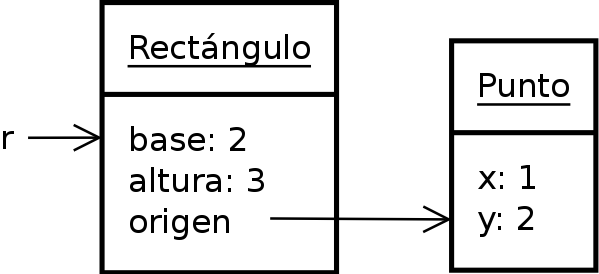
\includegraphics{graficos/15_Rectangulo_Punto}
\caption{Estado de las variables, al momento de crear el rectángulo}
\end{figure}

El punto que describe la posición de la esquina inferior izquierda del
rectángulo es un objeto \lstinline!Punto!. El atributo \lstinline!origen!
contiene una {\it referencia} a dicho objeto.

Utilizando el método \lstinline!trasladar!, podemos modificar el valor del
punto contenido dentro del rectángulo.

\begin{codigo-python-sn}
>>> r.trasladar(2,4)
>>> print r
Base: 2, Altura: 3, Esquina inf. izq.: (3, 6)
\end{codigo-python-sn}

También es posible directamente reemplazar el punto contenido, por un nuevo
punto.

\begin{codigo-python-sn}
>>> q = Punto(7,2)
>>> r.origen = q
>>> print r
Base: 2, Altura: 3, Esquina inf. izq.: (7, 2)
\end{codigo-python-sn}

Con lo cual el diagrama pasa a ser el de la Figura
\ref{rectangulo_punto_b}.

\begin{figure}[htb]
\label{rectangulo_punto_b}
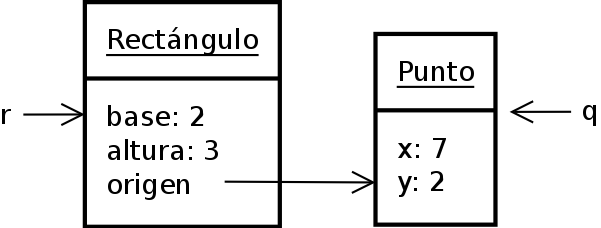
\includegraphics{graficos/15_Rectangulo_Punto_b}
\caption{Estado de las variables, luego de reemplazar el origen}
\end{figure}

\begin{observacion}
El \lstinline!Punto(1, 2)! y \lstinline!Punto(3,6)! que habían sido creados
previamente, están ahora fuera de uso, por lo que quedan a disposición de un
mecanismo de {\it recolección de basura}, que no es tema de esta materia,
que se encarga de juntar todos los pedazos de memoria que se descartan
durante la ejecución de un programa.
\end{observacion}

\section{Resumen}

\begin{itemize}
\item Se llama {\bf polimorfismo} a la posibilidad de obtener distintos
comportamientos mediante la invocación a métodos de un mismo nombre, pero de
clases distintas.

\item Se llama {\bf herencia} a la relación entre clases en la cual una es una
clase base y otra es una clase derivada, que {\it hereda} los métodos y
atributos de la clase base.

\item Se llama {\bf delegación} a la relación entre clases en la cual una clase
contiene como atributo a otra clase, y dentro de sus métodos realiza
invocaciones a los métodos de la clase contenida.

\item Se denomina {\bf referencia} a las variables que permiten acceder a
un determinado objeto, ya sea un atributo dentro de un objeto, o una
variable en una porción de código cualquiera.
\end{itemize}


\newpage
\section{Ejercicios}

\begin{extract}
Temas optativos para 2010 y 2011.
\end{extract}

\begin{ejercicio}
{\bf Papel, Birome, Marcador}
\begin{partes}
    \item Escribir una clase {\it Papel} que contenga un texto, un método {\it
escribir}, que reciba una cadena para agregar al texto, y el método {\it
\_\_str\_\_} que imprima el contenido del texto.
    \item Escribir una clase {\it Birome} que contenga una cantidad de tinta, y
un método {\it escribir}, que reciba un texto y un papel sobre el cual
escribir. Cada letra escrita debe reducir la cantidad de tinta contenida.
Cuando la tinta se acabe, debe lanzar una excepción.
    \item Escribir una clase {\it Marcador} que herede de Birome, y agregue el
método {\it recargar}, que reciba la cantidad de tinta a agregar.
\end{partes}
\end{ejercicio}


\begin{ejercicio}
Juego de Rol
\begin{partes}
    \item Escribir una clase {\it Personaje} que contenga los atributos {\it
vida}, {\it posicion} y {\it velocidad}, y los métodos {\it
recibir\_ataque}, que reduzca la vida según una cantidad recibida y lance
una excepción si la vida pasa a ser menor o igual que cero, y {\it
mover} que reciba una dirección y se mueva en esa dirección la cantidad
indicada por velocidad.
    \item Escribir una clase {\it Soldado} que herede de Personaje, y agregue
el atributo {\it ataque} y el método {\it atacar}, que reciba otro
personaje, al que le debe hacer el daño indicado por el atributo ataque.
    \item Escribir una clase {\it Campesino} que herede de Personaje, y agregue
el atributo {\it cosecha} y el método {\it cosechar}, que devuelva la
cantidad cosechada.
\end{partes}
\end{ejercicio}


% Copyright (C) 2008-2010 Rosita Wachenchauzer <rositaw@gmail.com>
%               Margarita Manterola <margamanterola@gmail.com>

% Esta obra est� licenciada de forma dual, bajo las licencias Creative
% Commons:
%  * Atribuci�n-Compartir Obras Derivadas Igual 2.5 Argentina
%    http://creativecommons.org/licenses/by-sa/2.5/ar/
%  * Atribuci�n-Compartir Obras Derivadas Igual 3.0 Unported
%    http://creativecommons.org/licenses/by-sa/3.0/deed.es_AR.
%
% A su criterio, puede utilizar una u otra licencia, o las dos.
% Para ver una copia de las licencias, puede visitar los sitios
% mencionados, o enviar una carta a Creative Commons,
% 171 Second Street, Suite 300, San Francisco, California, 94105, USA.

\chapter{Listas enlazadas}

En esta unidad, nos dedicaremos a construir nuestras propias listas, que
consistir�n de cadenas de objetos enlazadas mediante referencias, como las
vistas en la unidad anterior.

Si bien Python ya cuenta con sus propias listas, las listas enlazadas que
implementaremos en esta unidad nos resultar�n tambi�n �tiles.  

\section{Una clase sencilla de {\it vagones}}

En primer lugar, definiremos una clase muy simple, \lstinline!Nodo!, que se
comportar� como un vag�n: tendr� s�lo dos atributos: \lstinline!dato!, que
servir� para almacenar cualquier informaci�n, y \lstinline!prox!, que servir�
para poner una referencia al siguiente vag�n.

Adem�s, como siempre, implementaremos el constructor y el m�todo
\lstinline!__str__! para poder imprimir el contenido del nodo.

\begin{codigo-python-sn}
class Nodo(object):
    def __init__(self, dato=None, prox = None):
        self.dato = dato
        self.prox = prox
    def __str__(self):
        return str(self.dato)
\end{codigo-python-sn}

Ejecutamos este c�digo:

\begin{codigo-python-sn}
>>> v3=Nodo("Bananas")
>>> v2=Nodo("Peras", v3)
>>> v1=Nodo("Manzanas", v2)
>>> print v1
Manzanas
>>> print v2
Peras
>>> print v3
Bananas
\end{codigo-python-sn}

Con esto hemos generado la estructura de la Figura \ref{nodos}.

\begin{figure}[htb]
\label{nodos}
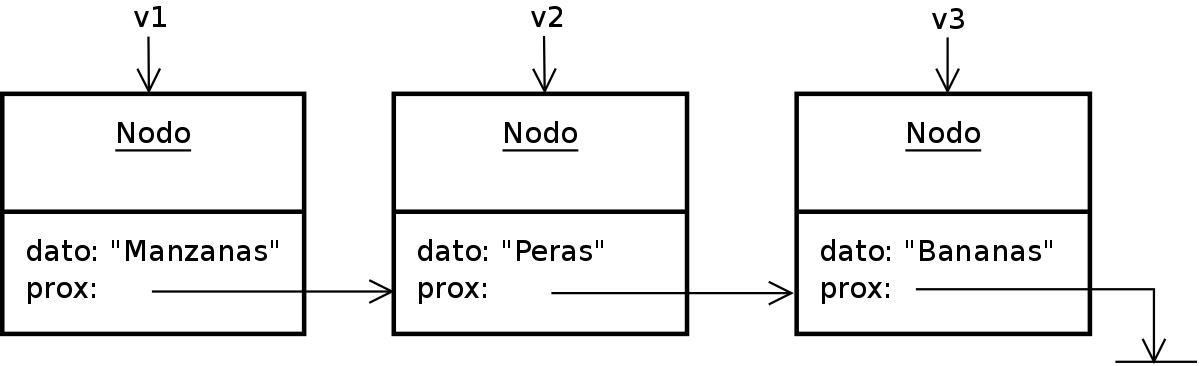
\includegraphics{graficos/16_Nodos}
\caption{Nodos enlazados}
\end{figure}

El atributo \lstinline!prox! de \lstinline!v3! tiene una referencia nula,
lo que indica que \lstinline!v3! es el �ltimo vag�n de nuestra estructura.

Hemos creado una lista en forma manual. Si nos interesa recorrerla, podemos
hacer lo siguiente:

\begin{codigo-python-sn}
def verLista(nodo):
    """ Recorre todos los nodos a trav�s de sus enlaces,
        mostrando sus contenidos. """

    # cicla mientras nodo no es None
    while nodo:
        # muestra el dato
        print nodo
        # ahora nodo apunta a nodo.prox
        nodo = nodo.prox
\end{codigo-python-sn}

\begin{codigo-python-sn}
>>> verLista(v1)
Manzanas
Peras
Bananas
\end{codigo-python-sn}

Es interesante notar que la estructura del recorrido de la lista es el
siguiente:

\begin{itemize}
\item Se le pasa a la funci�n s�lo la referencia al primer nodo.

\item El resto del recorrido se consigue siguiendo las cadena de
referencias dentro de los nodos.
\end{itemize}

Si se desea {\it desenganchar} un vag�n del medio de la lista, alcanza con
cambiar el enganche:

\begin{codigo-python-sn}
>>> v1.prox=v3
>>> verLista(v1)
Manzanas
Bananas
>>> v1.prox = None
>>> verLista(v1)
Manzanas
\end{codigo-python-sn}

De esta manera tambi�n se pueden generar estructuras impensables.

�Qu� sucede si escribimos \lstinline!v1.prox = v1!? La representaci�n es finita
y sin embargo en este caso \lstinline!verLista(v1)!  no termina m�s. Hemos
creado una {\it lista infinita}, tambi�n llamada {\it lista circular}.

% Este ejercicio no se entiende 
%\ejercicioc{�Cu�l es la mejor manera
%de tener siempre manzanas y peras a disposici�n de uno?}

\subsection{Caminos}

En una lista cualquiera, como las vistas antes, si seguimos las flechas
dadas por las referencias, obtenemos un {\it camino} en la lista.

Los caminos cerrados se denominan {\it ciclos}. Son ciclos, por ejemplo, la
autorreferencia de \lstinline|v1| a \lstinline|v1|, como as� tambi�n una
flecha de \lstinline|v1| a \lstinline|v2| seguida de una flecha de
\lstinline|v2| a \lstinline|v1|.

\begin{atencion}
Las listas circulares no tienen nada de malo en s� mismas,
mientras su representaci�n sea finita. El problema, en cambio, es que debemos tener
mucho cuidado al escribir programas para recorrerlas, ya que el recorrido
debe ser acotado (por ejemplo no habr�a problema en ejecutar un programa
que liste los 20 primeros nodos de una lista circular).

Cuando una funci�n recibe una lista y el recorrido no est� acotado
por programa, se debe aclarar en su precondici�n que la ejecuci�n de la misma terminar�
s�lo si la lista no contiene ciclos. �se es el caso de la funci�n
\lstinline|verLista(v1)|.
\end{atencion}

\subsection{Referenciando el principio de la lista}

Una cuesti�n no contemplada hasta el momento es la de mantener una referencia
a la lista completa. Por ahora para nosotros la lista es la colecci�n de nodos
que se enlazan a partir de \lstinline|v1|. Sin embargo puede suceder que queramos
borrar a \lstinline|v1| y continuar con el resto de la lista como la colecci�n de
nodos a tratar (en las listas de Python, \lstinline|del lista[0]| no nos hace perder
la referencia a \lstinline|lista|).

Para ello lo que haremos es asociar una referencia al principio de la lista,
que llamaremos \lstinline|lista|, y que mantendremos independientemente de cu�l sea
el nodo que est� al principio de la lista:

\begin{codigo-python-sn}
>>> v3=Nodo("Bananas")
>>> v2=Nodo("Peras", v3)
>>> v1=Nodo("Manzanas", v2)
>>> lista=v1
>>> verLista(lista)
Manzanas
Peras
Bananas
\end{codigo-python-sn}

Ahora s� estamos en condiciones de borrar el primer elemento de la lista
sin perder la identidad de la misma:

\begin{codigo-python-sn}
>>> lista=lista.prox
>>> verLista(lista)
Peras
Bananas
\end{codigo-python-sn}

\section{Tipos abstractos de datos}

Los tipos nuevos que hab�amos definido en unidades anteriores fueron tipos de
datos concretos: un punto se defin�a como un par ordenado de n�meros, un hotel
se defin�a por dos cadenas de caracteres (nombre y unicaci�n) y dos n�meros
(calidad y precio), etc.

Vamos a ver ahora una nueva manera de definir datos: por las
operaciones que tienen y por lo que tienen que hacer esas
operaciones (cu�l es el resultado esperado de esas operaciones).

Esa manera de definir datos se conoce como {\it tipos abstractos de datos} o
{\it TADs}.

Lo novedoso de este enfoque respecto del anterior es que en general se puede
encontrar m�s de una representaci�n mediante tipos concretos para representar
el mismo TAD, y que se puede elegir la representaci�n m�s conveniente en cada
caso, seg�n el contexto de uso.

Los programas que los usan hacen referencia a las operaciones que tienen, no a
la representaci�n, y por lo tanto ese programa sigue funcionando si se cambia
la representaci�n.

Dentro del ciclo de vida de un TAD hay dos fases: la programaci�n del TAD y
la construcci�n de los programas que lo usan.

Durante la fase de programaci�n del TAD, habr� que elegir una
representaci�n, y luego programar cada uno de los m�todos sobre esa
representaci�n.

Durante la fase de construcci�n de los programas, no ser� relevante para el
programador que utiliza el TAD c�mo est� implementado, sino �nicamente los
m�todos que posee.

\begin{observacion}
Utilizando el concepto de \emph{interfaz} visto en la unidad anterior, podemos
decir que a quien utilice el TAD s�lo le interesar� la interfaz que �ste
posea.
\end{observacion}

\section{La clase {\tt ListaEnlazada}}

Bas�ndonos en los nodos implementados anteriormente, pero buscando
deslindar al programador que desea usar la lista de la responsabilidad de
manipular las referencias, definiremos ahora la clase
\lstinline!ListaEnlazada!, de modo tal que no haya que operar mediante las
referencias internas de los nodos, sino que se lo pueda hacer a trav�s de
operaciones de lista.

M�s all� de la implementaci�n en particular, se podr� notar que implementaremos
los mismos m�todos de las listas de Python, de modo que m�s all� del
funcionamiento interno, ambas ser�n {\bf listas}. 

Definimos a continuaci�n las operaciones que inicialmente deber� cumplir la
clase \lstinline!ListaEnlazada!.

\begin{itemize}
\item \lstinline|__str__|, para mostrar la lista.

\item \lstinline|__len__|, para calcular la longitud de la lista.

\item \lstinline|append(x)|, para agregar un elemento al final de la lista.

\item \lstinline|insert(i, x)|, para agregar el elemento \lstinline!x! en la
posici�n \lstinline!i! (levanta una excepci�n si la posici�n \lstinline!i! es
inv�lida).

\item \lstinline|remove(x)|, para eliminar la primera aparici�n de
\lstinline!x! en la lista (levanta una excepci�n si \lstinline!x! no est�).

\item \lstinline|pop([i])|, para borrar el elemento que est� en la posici�n
\lstinline!i! y devolver su valor. Si no se especifica el valor de
\lstinline!i!, \lstinline|pop()| elimina y devuelve el elemento que est� en
el �ltimo lugar de la lista (levanta una excepci�n si se hace referencia a
una posici�n no v�lida de la lista).

\item \lstinline|index(x)|, devuelve la posici�n de la primera aparici�n de
\lstinline!x! en la lista (levanta una excepci�n si \lstinline!x! no est�).
\end{itemize}

M�s adelante podr�n agregarse a la lista otros m�todos que tambi�n est�n
implementados por las listas de Python.

Valen ahora algunas consideraciones m�s antes de empezar a implementar la clase:

\begin{itemize}

\item Por lo dicho anteriormente, es claro que la lista deber� tener como
atributo la referencia al primer nodo que la compone.

\item Como vamos a incluir un m�todo \lstinline|__len__|, consideramos que no
tiene sentido recorrer la lista cada vez que se lo llame, para contar
cu�ntos elementos tiene, alcanza con agregar un atributo m�s (la longitud
de la lista), que se inicializa en $0$ cuando se crea la lista vac�a, se
incrementa en $1$ cada vez que se agrega un elemento y se decrementa en $1$
cada vez que se borra un elemento.

\item Por otro lado, como vamos a incluir todas las operaciones de listas
que sean necesarias para operar con ellas, no es necesario que la clase
\lstinline!Nodo! est� disponible para que otros programadores puedan
modificar (y romper) las listas a voluntad usando operaciones de nodos. Para eso
incluiremos la clase \lstinline!Nodo! de manera {\it privada} (es
decir oculta), de modo que la podamos usar nosotros como due�os
(fabricantes) de la clase, pero no cualquier programador que utilice la
lista.
\end{itemize}

Python tiene una convenci�n para hacer que atributos, m�todos o clases
dentro de una clase dada no puedan ser usados por los usuarios, y s�lo
tengan acceso a ellos quienes programan la clase: su nombre tiene que
empezar con un gui�n bajo y terminar sin gui�n bajo. As� que para hacer que
los nodos sean privados, nombraremos a esa clase como \lstinline|_Nodo|, y
la dejaremos tal como hasta ahora.

\begin{observacion}
Se trata s�lo de una convenci�n, a�n con el nombre \lstinline!_Nodo! la
clase est� disponible, pero respetaremos esa convenci�n de aqu� en adelnte.
\end{observacion}

\subsection{Construcci�n de la lista}

Empezamos escribiendo la clase con su constructor.

\begin{codigo-python-sn}
class ListaEnlazada(object):
    " Modela una lista enlazada, compuesta de Nodos. "

    def __init__(self):
        """ Crea una lista enlazada vac�a. """
        # prim: apuntar� al primer nodo - None con la lista vac�a
        self.prim = None
        # len: longitud de la lista - 0 con la lista vac�a 
        self.len = 0
\end{codigo-python-sn}

Nuestra estructura ahora ser� como la representada por la Figura
\ref{lista_enlazada}.

\begin{figure}[htb]
\label{lista_enlazada}
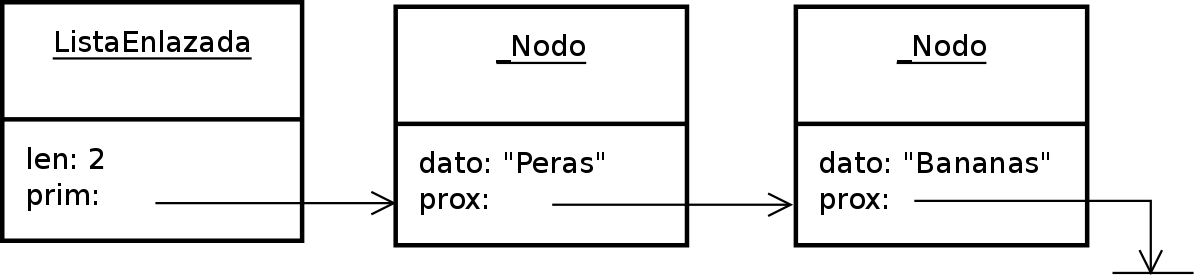
\includegraphics{graficos/16_ListaEnlazada}
\caption{Una lista enlazada}
\end{figure}

\ejercicioc{Escribir los m�todos \lstinline!__str__! y \lstinline!__len__!
para la lista}.

\begin{sabias_que}
Una caracter�stica importante de la implementaci�n de lista enlazadas es que
borrar el primer elemento es una operaci�n de {\it tiempo constante}, es
decir que no depende del largo de la lista, a diferencia de las listas de
Python, en las que esta operaci�n requiere un {\it tiempo proporcional a la
longitud de la lista}). 

Sin embargo no todo es tan positivo: el acceso a la posici�n {\tt p} se realiza
en {\it tiempo proporcional a p}, mientras que en las listas de Python esta
operaci�n se realiza en {\it tiempo constante}.

Conociendo las ventajas y desventajas podremos elegir el tipo de lista que
necesitemos seg�n los requerimientos de cada problema.
\end{sabias_que}

\subsection{Eliminar un elemento de una posici�n}

Analizaremos a continuaci�n \lstinline|pop([i])|, que borra el elemento que
est� en la posici�n \lstinline!i! y devuelve su valor. Si no se especifica
el valor de \lstinline!i!, \lstinline|pop()| elimina y devuelve el elemento
que est� en el �ltimo lugar de la lista.  Por otro lado, levanta una
excepci�n si se hace referencia a una posici�n no v�lida de la lista.

Dado que se trata de una funci�n con cierta complejidad, separaremos el
c�digo en las diversas consideraciones a tener en cuenta.

\begin{itemize}

\item Si la posici�n es inv�lida (\lstinline!i! menor que $0$ o mayor o
igual a la longitud de la lista), se considera error y se levanta la
excepci�n ValueError.

Esto se resuelve con este fragmento de c�digo:

\begin{codigo-python-sn}
        # Verificaci�n de los l�mites
        if (i < 0) or (i >= self.len):
            raise IndexError("�ndice fuera de rango")
\end{codigo-python-sn}

\item Si no se indica posici�n, \lstinline!i! toma la �ltima posici�n de la lista.

Esto se resuelve con este fragmento de c�digo:
\begin{codigo-python-sn}
        # Si no se recibi� i, se devuelve el �ltimo.
        if i == None:
            i = self.len - 1
\end{codigo-python-sn}

\item Cuando la posici�n es $0$ se trata de un caso particular, ya que en ese
caso, adem�s de borrar el nodo, hay que cambiar la referencia de
\lstinline!self.prim! para que apunte al nodo siguiente.  Es decir, pasar de
\lstinline!self.prim! $\rightarrow$ nodo0 $\rightarrow$ nodo1 a
\lstinline!self.prim! $\rightarrow$ nodo1).

Esto se resuelve con este fragmento de c�digo:

\begin{codigo-python-sn}
        # Caso particular, si es el primero, 
        # hay que saltear la cabecera de la lista
        if i == 0:
            dato = self.prim.dato
            self.prim = self.prim.prox
\end{codigo-python-sn}

\item Vemos ahora el caso general:

Mediante un ciclo, se deben ubicar los nodos {\it npi - 1} y {\it npi} que
est�n en las posiciones $i-1$ e $i$ de la lista, respectivamente, de modo de
poder ubicar no s�lo el nodo que se borrar�, sino tambi�n estar en condiciones
de saltear el nodo borrado en los enlaces de la lista.  La lista debe pasar de
contener el camino {\it npi - 1} $\rightarrow$ {\it npi} $\rightarrow$ {\it
npi.prox} a contener el camino {\it npi-1} $\rightarrow$ {\it npi.prox}.

Nos basaremos un esquema muy simple (y �til) que se denomina {\it m�quina de parejas}:

Si nuestra secuencia tiene la forma ABCDE, se itera sobre ella de modo de
tener las parejas AB, BC, CD, DE. En la pareja XY, llamaremos a X el {\it elemento anterior}
y a Y el {\it elemento actual}. En general estos ciclos terminan o bien cuando
no hay m�s parejas que formar, o bien cuando el elemento actual cumple con una determinada
condici�n.

En nuestro problema, tenemos la siguiente situaci�n:

\begin{itemize}
\item Las parejas son parejas de nodos.

\item Para avanzar en la secuencia se usa la referencia al pr�ximo nodo de la lista.

\item La condici�n de terminaci�n es siempre que la posici�n del nodo en la
lista sea igual al valor buscado.  En este caso particular no debemos
preocuparnos por la terminaci�n de la lista porque la validez del �ndice
buscado ya fue verificada m�s arriba.
\end{itemize}

Esta es la porci�n de c�digo correspondiente a la b�squeda:

\begin{codigo-python-sn}
            n_ant = self.prim
            n_act = n_ant.prox
            for pos in xrange(1, i):
                n_ant = n_act
                n_act = n_ant.prox
\end{codigo-python-sn}

Al finalizar el ciclo, \lstinline!n_ant! ser� una referencia al nodo $i-1$ y
\lstinline!n_act! una referencia al nodo $i$.

Una vez obtenidas las referencias, se obtiene el dato y se cambia el camino
seg�n era necesario:

\begin{codigo-python-sn}
            # Guarda el dato y elimina el nodo a borrar
            dato = n_act.dato
            n_ant.prox = n_act.prox
\end{codigo-python-sn}


\item Finalmente, en todos los casos de �xito, se debe devolver el dato que conten�a
el nodo eliminado y decrementar la longitud en 1:

\begin{codigo-python-sn}
        # hay que restar 1 de len  
        self.len -= 1
        # y devolver el valor borrado
        return dato
\end{codigo-python-sn}

\end{itemize}

Finalmente, en el C�digo \ref{lista_enlazada_pop} se incluye el c�digo completo
del m�todo \lstinline!pop!.

\begin{codigo}{pop}{M�todo pop de la lista enlazada}
\label{lista_enlazada_pop}
\begin{codigo-python}
   def pop(self, i = None):
        """ Elimina el nodo de la posici�n i, y devuelve el dato contenido.
            Si i est� fuera de rango, se levanta la excepci�n IndexError.
            Si no se recibe la posici�n, devuelve el �ltimo elemento. """

        # Si no se recibi� i, se devuelve el �ltimo.
        if i is None:
            i = self.len - 1

        # Verificaci�n de los l�mites
        if not (0 <= i < self.len):
            raise IndexError("�ndice fuera de rango")

        # Caso particular, si es el primero, 
        # hay que saltear la cabecera de la lista
        if i == 0:
            dato = self.prim.dato
            self.prim = self.prim.prox

        # Para todos los dem�s elementos, busca la posici�n
        else:
            n_ant = self.prim
            n_act = n_ant.prox
            for pos in xrange(1, i):
                n_ant = n_act
                n_act = n_ant.prox

            # Guarda el dato y elimina el nodo a borrar
            dato = n_act.dato
            n_ant.prox = n_act.prox

        # hay que restar 1 de len  
        self.len -= 1
        # y devolver el valor borrado
        return dato
\end{codigo-python}
\end{codigo}

\subsection{Eliminar un elemento por su valor}

An�logamente se resuelve \lstinline|remove(self,x)|, que debe eliminar la
primera aparici�n de \lstinline!x! en la lista, o bien levantar una excepci�n
si \lstinline!x! no se encuentra en la lista.

Nuevamente, dado que se trata de un m�todo de cierta complejidad, lo
resolveremos por partes, teniendo en cuenta los casos particulares y el caso
general.

\begin{itemize}

\item Los casos particulares son: la lista vac�a, que es un error y hay que
levantar una excepci�n; y el caso en el que x est� en el primer nodo, en este
caso hay que saltear el primer nodo desde la cabecera de la lista.

El fragmento de c�digo que resuelve estos casos es:

\begin{codigo-python-sn}
        if self.len == 0:
            # Si la lista est� vac�a, no hay nada que borrar.
            raise ValueError("Lista vac�a")

        # Caso particular, x esta en el primer nodo
        elif self.prim.dato == x:
            # Se descarta la cabecera de la lista
            self.prim = self.prim.prox
\end{codigo-python-sn}

\item El caso general tambi�n implica un recorrido con m�quina de parejas, s�lo
que esta vez la condici�n de terminaci�n es: o bien la lista se termin� o bien
encontramos un nodo con el valor (\lstinline!x!) buscado.

\begin{codigo-python-sn}
            # Obtiene el nodo anterior al que contiene a x (n_ant)
            n_ant = self.prim
            n_act = n_ant.prox
            while n_act != None and n_act.dato != x:
                n_ant = n_act
                n_act = n_ant.prox
\end{codigo-python-sn}

En este caso, al terminarse el ciclo ser� necesario corroborar si se termin�
porque lleg� al final de la lista, y de ser as� levantar una excepci�n; o si se
termin� porque encontr� el dato, y de ser as� eliminarlo.

\begin{codigo-python-sn}
            # Si no se encontr� a x en la lista, levanta la excepci�n
            if n_act == None:
                raise ValueError("El valor no est� en la lista.")

            # Si encontr� a x, debe pasar de n_ant -> n_x -> n_x.prox
            # a n_ant -> n_x.prox
            else:
                n_ant.prox = n_act.prox
\end{codigo-python-sn}

\item Finalmente, en todos los casos de �xito debemos decrementar en 1 el valor
de \lstinline|self.len|.

\end{itemize}

En el C�digo \ref{lista_enlazada_remove} se incluye el c�digo completo
del m�todo \lstinline!remove!.

\begin{codigo}{remove}{M�todo remove de la lista enlazada}
\label{lista_enlazada_remove}
\begin{codigo-python}
    def remove(self, x):
        """ Borra la primera aparici�n del valor x en la lista.
            Si x no est� en la lista, levanta ValueError """

        if self.len == 0:
            # Si la lista est� vac�a, no hay nada que borrar.
            raise ValueError("Lista vac�a")

        # Caso particular, x esta en el primer nodo
        elif self.prim.dato == x:
            # Se descarta la cabecera de la lista
            self.prim = self.prim.prox

        # En cualquier otro caso, hay que buscar a x
        else:
            # Obtiene el nodo anterior al que contiene a x (n_ant)
            n_ant = self.prim
            n_act = n_ant.prox
            while n_act != None and n_act.dato != x:
                n_ant = n_act
                n_act = n_ant.prox

            # Si no se encontr� a x en la lista, levanta la excepci�n
            if n_act == None:
                raise ValueError("El valor no est� en la lista.")

            # Si encontr� a x, debe pasar de n_ant -> n_x -> n_x.prox
            # a n_ant -> n_x.prox
            else:
                n_ant.prox = n_act.prox

        # Si no levant� excepci�n, hay que restar 1 del largo
        self.len -= 1
\end{codigo-python}
\end{codigo}

\subsection{Insertar nodos}

Debemos programar ahora \lstinline|insert(i, x)|, que debe agregar el elemento
\lstinline!x! en la posici�n \lstinline!i!  (y levantar una excepci�n si la
posici�n \lstinline!i! es inv�lida).

Veamos qu� debemos tener en cuenta para programar esta funci�n.

\begin{itemize}

\item Si se intenta insertar en una posici�n menor que cero o mayor que la
longitud de la lista debe levantarse una excepci�n.

\begin{codigo-python-sn}
        if (i > self.len) or (i < 0):
            # error
            raise IndexError("Posici�n inv�lida")
\end{codigo-python-sn}

\item Para los dem�s casos, hay que crear un nodo, que ser� el que se insertar�
en la posici�n que corresponda. Construimos un nodo \lstinline|nuevo| cuyo
\lstinline|dato| sea \lstinline|x|.

\begin{codigo-python-sn}
        # Crea nuevo nodo, con x como dato:
        nuevo = _Nodo(x)
\end{codigo-python-sn}

\item Si se quiere insertar en la posici�n 0, hay que cambiar la referencia de
\lstinline|self.prim|.

\begin{codigo-python-sn}
        # Insertar al principio (caso particular)
        if i == 0:
            # el siguiente del nuevo pasa a ser el que era primero
            nuevo.prox = self.prim
            # el nuevo pasa a ser el primero de la lista
            self.prim = nuevo
\end{codigo-python-sn}

\item Para los dem�s casos, nuevamente ser� necesaria la m�quina de parejas.
Obtenemos el nodo anterior a la posici�n en la que queremos insertar.

\begin{codigo-python-sn}
        # Insertar en cualquier lugar > 0
        else:
            # Recorre la lista hasta llegar a la posici�n deseada
            n_ant = self.prim
            for pos in xrange(1,i):
                n_ant = n_ant.prox

            # Intercala nuevo y obtiene n_ant -> nuevo -> n_ant.prox
            nuevo.prox = n_ant.prox
            n_ant.prox = nuevo
\end{codigo-python-sn}

\item En todos los casos de �xito se debe incrementar en 1 la longitud de la lista.
\begin{codigo-python-sn}
        # En cualquier caso, incrementar en 1 la longitud
        self.len += 1
\end{codigo-python-sn}

\end{itemize}

En el C�digo \ref{lista_enlazada_insert} se incluye el c�digo resultante
del m�todo \lstinline!insert!.

\begin{codigo}{insert}{M�todo insert de la lista enlazada}
\label{lista_enlazada_insert}
\begin{codigo-python}
    def insert(self, i, x):
        """ Inserta el elemento x en la posici�n i.
            Si la posici�n es inv�lida, levanta IndexError """

        if (i > self.len) or (i < 0):
            # error
            raise IndexError("Posici�n inv�lida")

        # Crea nuevo nodo, con x como dato:
        nuevo = _Nodo(x)

        # Insertar al principio (caso particular)
        if i == 0:
            # el siguiente del nuevo pasa a ser el que era primero
            nuevo.prox = self.prim
            # el nuevo pasa a ser el primero de la lista
            self.prim = nuevo

        # Insertar en cualquier lugar > 0
        else:
            # Recorre la lista hasta llegar a la posici�n deseada
            n_ant = self.prim
            for pos in xrange(1,i):
                n_ant = n_ant.prox

            # Intercala nuevo y obtiene n_ant -> nuevo -> n_ant.prox
            nuevo.prox = n_ant.prox
            n_ant.prox = nuevo

        # En cualquier caso, incrementar en 1 la longitud
        self.len += 1
\end{codigo-python}
\end{codigo}

\ejercicioc{Completar la clase \lstinline|ListaEnlazada| con los m�todos que
faltan: \lstinline|append| e \lstinline|index|}.

\ejercicioc{En los bucles de {\it m�quina de parejas} mostrados
anteriormente, no siempre es necesario tener la referencia al nodo actual,
puede alcanzar con la referencia al nodo anterior.  Donde sea posible,
eliminar la referencia al nodo actual.  Una vez hecho esto, analizar el
c�digo resultante, �Es m�s elegante?}

\ejercicioc{\label{append_constante} {\bf Mantenimiento:} Con esta representaci�n conseguimos que la
inserci�n en la posici�n 0 se realice en tiempo constante, sin embargo ahora
\lstinline|append| es lineal en la longitud de la lista. Como nuestro cliente
no est� satisfecho con esto debemos agregar un atributo m�s a los objetos de la
clase, la referencia al �ltimo nodo, y modificar \lstinline|append| para que se
pueda ejecutar en tiempo constante. Por supuesto que adem�s hay que modificar
todos los m�todos de la clase para que se mantenga la propiedad de que ese
atributo siempre es una referencia al �timo nodo.}

\section{Invariantes de objetos}

Los invariantes son condiciones que deben ser siempre ciertas.  Hemos visto
anteriormente los invariantes de ciclos, que son condiciones que deben
permanecer ciertas durante la ejecuci�n de un ciclo.  Existen tambi�n los
invariantes de objetos, que son condiciones que deben ser ciertas a lo
largo de toda la existencia de un objeto.

La clase \lstinline!ListaEnlazada! presentada en la secci�n anterior,
cuenta con dos invariantes que siempre debemos mantener.  Por un lado, el
atributo \lstinline!len! debe contener siempre la cantidad de nodos de la
lista.  Es decir, siempre que se modifique la lista, agregando o quitando
un nodo, se debe actualizar \lstinline!len! como corresponda.

Por otro lado, el atributo \lstinline!prim! referencia siempre al primer
nodo de la lista, si se agrega o elimina este primer nodo, es necesario
actualizar esta referencia.

Cuando se desarrolla una estructura de datos, como la lista enlazada, es
importante destacar cu�les ser�n sus invariantes, ya que en cada m�todo
habr� que tener especial cuidado de que los invariantes permanezcan siempre
ciertos.

As�, si como se pidi� en el ejercicio \ref{append_constante}, se modifica
la lista para que la inserci�n al final pueda hacerse en tiempo constante,
se est� agregando a la lista un nuevo invariante (un atributo de la lista
que apunte siempre al �ltimo elemento) y no es s�lo el m�todo
\lstinline!append! el que hay que modificar, sino todos los m�todos que
puedan de una u otra forma cambiar la referencia al �ltimo elemento de la
lista.

\section{Otras listas enlazadas}

Las listas presentadas hasta aqu� son las {\it listas simplemente
enlazadas}, que son sencillas y �tiles cuando se quiere poder insertar o
eliminar nodos de una lista en tiempo constante.

Existen otros tipos de listas enlazadas, cada uno con sus ventajas y
desventajas.

\subsection*{Listas doblemente enlazadas}

Las listas doblemente enlazadas son aquellas en que los nodos cuentan no
s�lo con una referencia al siguiente, sino tambi�n con una referencia al
anterior.  Esto permite que la lista pueda ser recorrida en ambas
direcciones.

En una lista doblemente enlazada, es posible, por ejemplo, eliminar un
nodo, teniendo �nicamente ese nodo, sin necesidad de saber tambi�n cu�l es
el anterior.

Entre las desventajas podemos mencionar que al tener que mantener dos
referencias el c�digo se vuelve m�s complejo, y tambi�n que ocupa m�s
espacio en memoria.

\subsection*{Listas circulares}

Las listas circulares, que ya fueron mencionadas al comienzo de esta
unidad, son aquellas en las que el �ltimo nodo contiene una referencia al
primero.  Pueden ser tanto simplemente como doblemente enlazadas.

Se las utiliza para modelar situaciones en las cuales los elementos no
tienen un primero o un �ltimo, sino que forman una cadena infinita, que se
recorre una y otra vez.

\begin{sabias_que}
Un ejemplo de uso de las listas circulares es dentro del kernel Linux.  La
mayor�a de las listas utilizadas por este kernel son circulares, ya que la
mayor�a de los datos a los que se quiere acceder son datos que no tienen un
orden en particular.

Por ejemplo, la lista de tareas que se est�n ejecutando es una lista
circular.  El {\it scheduler} del kernel permite que cada tarea utilice el
procesador durante una porci�n de tiempo y luego pasa a la siguiente; y al
llegar a la {\it �ltima} vuelve a la {\it primera}, ya que la ejecuci�n de
tareas no se termina.
\end{sabias_que}

% TODO: esto se da en la pr�ctica... C�mo lo indicamos?
\section{Iteradores}

En la unidad anterior se hizo referencia a que todas las secuencias
pueden ser recorridas mediante una misma estructura (
\lstinline!for variable in secuencia!), ya que todas implementan el m�todo
especial \lstinline!__iter__!.  Este m�todo debe devolver un {\it iterador}
capaz de recorrer la secuencia como corresponda.

\begin{observacion}
Un iterador es un objeto que permite recorrer uno a uno los elementos
almacenados en una estructura de datos, y operar con ellos.
\end{observacion}

En particular, en Python, los iteradores tienen que implementar un m�todo
\lstinline!next! que debe devolver los elementos, de a uno por vez,
comenzando por el primero.  Y al llegar al final de la estructura, debe
levantar una excepci�n de tipo \lstinline!StopIteration!.

Es decir que las siguientes estructuras son equivalentes
\begin{codigo-python-sn}
for elemento in secuencia:
	# hacer algo con elemento
\end{codigo-python-sn}

\begin{codigo-python-sn}
iterador = iter(secuencia)
while True:
    try:
        elemento = iterador.next()
    except StopIteration:
        break
    # hacer algo con elemento
\end{codigo-python-sn}

En particular, si queremos implementar un iterador para la lista enlazada,
la mejor soluci�n implica crear una nueva clase,
\lstinline!_IteradorListaEnlazada!, que implemente el m�todo
\lstinline!next()! de la forma apropiada.

\begin{atencion}
Utilizamos la notaci�n de clase privada, utilizada tambi�n para la clase
\lstinline!_Nodo!, ya que si bien se devolver� el iterador cuando sea
necesario, un programador externo no deber�a construir el iterador sin
pasar a trav�s de la lista enlazada.
\end{atencion}

Para inicializar la clase, lo �nico que se necesita es una referencia al
primer elemento de la lista.  

\begin{codigo-python-sn}
class _IteradorListaEnlazada(object):
    " Iterador para la clase ListaEnlazada "
    def __init__(self, prim):
        """ Constructor del iterador.  
            prim es el primer elemento de la lista. """
        self.actual = prim
\end{codigo-python-sn}

A partir de all�, el iterador ir� avanzando a trav�s de los elementos de la
lista mediante el m�todo \lstinline!next!.  Para verificar que no se haya
llegado al final de la lista, se corroborar� que la referencia
\lstinline!self.actual! sea distinta de \lstinline!None!.

\begin{codigo-python-sn}
        if self.actual == None:
            raise StopIteration("No hay m�s elementos en la lista")
\end{codigo-python-sn}

Una vez que se pas� la verificaci�n, la primera llamada a \lstinline!next!
debe devolver el primer elemento, pero tambi�n debe avanzar, para que la
siguiente llamada devuelva el siguiente elemento.  Por ello, se utiliza la
estructura {\it guardar, avanzar, devolver}.

\begin{codigo-python-sn}
        # Guarda el dato
        dato = self.actual.dato
        # Avanza en la lista
        self.actual = self.actual.prox
        # Devuelve el dato
        return dato
\end{codigo-python-sn}

En el C�digo \ref{iterador_enlazada} se puede ver el c�digo completo del
iterador.

\begin{codigo}{\_IteradorListaEnlazada}{Un iterador para la lista enlazada}
\label{iterador_enlazada}
\begin{codigo-python}
class _IteradorListaEnlazada(object):
    " Iterador para la clase ListaEnlazada "
    def __init__(self, prim):
        """ Constructor del iterador.  
            prim es el primer elemento de la lista. """
        self.actual = prim

    def next(self):
        """ Devuelve uno a uno los elementos de la lista. """
        if self.actual == None:
            raise StopIteration("No hay m�s elementos en la lista")

        # Guarda el dato
        dato = self.actual.dato
        # Avanza en la lista
        self.actual = self.actual.prox
        # Devuelve el dato
        return dato
\end{codigo-python}
\end{codigo}

Finalmente, una vez que se tiene el iterador implementado, es necesario
modificar la clase \lstinline!ListaEnlazada! para que devuelva el iterador
cuando se llama al m�todo \lstinline!__iter__!.

\begin{codigo-python-sn}
    def __iter__(self):
        " Devuelve el iterador de la lista. "
        return _IteradorListaEnlazada(self.prim)
\end{codigo-python-sn}

Con todo esto ser� posible recorrer nuestra lista con la estructura a la
que estamos acostumbrados.

\begin{codigo-python-sn}
>>> l = ListaEnlazada()
>>> l.append(1)
>>> l.append(3)
>>> l.append(5)
>>> for valor in l:
...     print valor
... 
1
3
5
\end{codigo-python-sn}

\section{Resumen}

\begin{itemize}

\item Un {\bf tipo abstracto de datos} (TAD) es un tipo de datos que est�
definido por las operaciones que contiene y c�mo se comportan (su {\it
interfaz}), no por la forma en la que esas operaciones est�n implementadas.

\item Una {\bf lista enlazada} es una implementaci�n del TAD {\it lista}.
Se trata de una lista compuesta por nodos, en la que
cada nodo contiene un dato y una referencia al nodo que le sigue.

\item En las listas enlazadas, es {\it barato} insertar o eliminar
elementos, ya que simplemente se deben alterar un par de referencias; pero
es {\it caro} acceder a un elemento en particular, ya que es necesario
pasar por todos los anteriores para llegar a �l.

\item Tanto al insertar como al remover elementos de una lista enlazada, se
utiliza la t�cnica de {\it m�quina de parejas}, mediante la cual se va
recorriendo la lista hasta encontrar el lugar apropiado donde operar con
las referencias.

\item Una {\bf lista doblemente enlazada} es aquella cuyos nodos adem�s del
dato contienen una referencia al nodo anterior y otra al nodo siguiente, de
modo que se la puede recorrer en ambos sentidos.

\item Una {\bf lista circular} es aquella en la que el �ltimo nodo contiene
una referencia al primero, y puede ser recorrida infinitamente.

\item Un {\bf iterador} es un objeto que permite recorrer uno a uno los
elementos de una secuencia.

\end{itemize}


\newpage
\section{Ejercicios}

\ejercicio{
Agregar a la clase {\it ListaEnlazada} un m�todo \verb!next! que vaya
devolviendo uno a uno cada elemento de la lista, desde el primero hasta el
�ltimo.  Al llegar al final de la lista debe levantar una excepci�n de la
clase {\it StopIteration}.  Para el correcto funcionamiento de este m�todo, �es
necesario agregar un atributo adicional a la clase?
}

\ejercicio{
Utilizando el m�todo \verb!next! del ejercicio anterior, redefinir el
m�todo \verb!__str__! de {\it ListaEnlazada}, para que se genere una salida
legible de lo que contiene la lista, similar a las listas de python. \\
{\bf Nota}: este m�todo debe devolver una cadena, no imprimirla por
pantalla.
}

\ejercicio{
Agregar a {\it ListaEnlazada} un m�todo \verb!extend! que reciba una {\it
ListaEnlazada} y agregue a la lista actual los elementos que se encuentran
en la lista recibida.
}

% No es un buen ejemplo que LE Ordenada herede de LE ya que se tiene que bloquear 
% o redefinir el significado del m�todo append.
% 
%\ejercicioc{
%Escribir una clase {\it ListaEnlazadaOrdenada} que herede de {\it
%ListaEnlazada}, redefiniendo el m�todo \verb!insert! para que inserte los
%elementos de forma ordenada, y el m�todo \verb!append! para que no permita
%la inserci�n al final.
%}

\ejercicio{
Una {\bf lista circular} es una lista cuyo �ltimo nodo est� ligado al primero,
de modo que es posible recorrerla infinitamente.  \\
Escribir la clase {\it ListaCircular}, incluyendo los m�todos \verb!insert!,
\verb!append!, \verb!remove! y \verb!pop!.
}

\ejercicio{
Una {\bf lista doblemente enlazada} es una lista en la cual cada nodo tiene
una referencia al anterior adem�s de al pr�ximo de modo que es posible
recorrerla en ambas direcciones. \\ 
Escribir la clase {\it ListaDobleEnlazada}, incluyendo los m�todos
\verb!insert!, \verb!append!, \verb!remove! y \verb!pop!.
}

\ejercicio{
Escribir un m�todo de la clase {\it ListaEnlazada} que invierta el orden
de la lista (es decir, el primer elemento queda como �ltimo y
viceversa, y se invierte la direcci�n de todos los enlaces). \\
{\bf Nota}: operar directamente sobre los elementos de la lista.
}


% Copyright (C) 2008-2010 Rosita Wachenchauzer <rositaw@gmail.com>
%               Margarita Manterola <margamanterola@gmail.com>

% Esta obra está licenciada de forma dual, bajo las licencias Creative
% Commons:
%  * Atribución-Compartir Obras Derivadas Igual 2.5 Argentina
%    http://creativecommons.org/licenses/by-sa/2.5/ar/
%  * Atribución-Compartir Obras Derivadas Igual 3.0 Unported
%    http://creativecommons.org/licenses/by-sa/3.0/deed.es_AR.
%
% A su criterio, puede utilizar una u otra licencia, o las dos.
% Para ver una copia de las licencias, puede visitar los sitios
% mencionados, o enviar una carta a Creative Commons,
% 171 Second Street, Suite 300, San Francisco, California, 94105, USA.

\chapter{Pilas y colas}

En esta unidad veremos dos ejemplos de tipos abstractos de datos, de los más
clásicos: {\it pilas} y {\it colas}.

\section{Pilas}

Una {\it pila} es un TAD que tiene las siguientes operaciones (se describe también la acción que
lleva adelante cada operación):

\begin{itemize}
\item \lstinline+__init__+: Inicializa una pila nueva, vacía.

\item \lstinline!apilar!: Agrega un nuevo elemento a la pila.

\item \lstinline!desapilar!: Elimina el tope de la pila y lo devuelve.
El elemento que se devuelve es siempre el último que se agregó.

\item \lstinline!es_vacia!: Devuelve \lstinline!True! o \lstinline!False!
según si la pila está vacía o no.

\end{itemize}

El comportamiento de una pila se puede describir mediante la frase
``Lo último que se apiló es lo primero que se usa'', que es exactamente lo que
uno hace con una pila (de platos por ejemplo): en una pila de platos uno sólo
puede ver la apariencia completa del plato de arriba, y sólo puede tomar el
plato de arriba (si se intenta tomar un plato del medio de la pila lo más
probable es que alguno de sus vecinos, o él mismo, se arruine).

Como ya se dijo, al crear un tipo abstracto de datos, es importante decidir
cuál será la representación a utilizar.  En el caso de la pila, si bien puede
haber más de una representación, por ahora veremos la más sencilla:
representaremos una pila mediante una lista de Python.

Sin embargo, para los que construyen programas que usan un TAD vale el
siguiente llamado de atención:

\begin{atencion}
Al usar esa pila dentro de un programa, deberemos ignorar que se está
trabajando sobre una lista: solamente podremos usar los métodos de pila.

Si alguien viola este principio, y usa la representación dentro del
programa usuario, termina por recibir el peor castigo imaginable para un/a
programador/a: sus programas pueden dejar de funcionar el cualquier
momento, tan pronto como quien produce del TAD decida cambiar, aunque sea
sutilmente, dicha representación.
\end{atencion}

\subsection{Pilas representadas por listas}

Definiremos una clase \lstinline!Pila! con un atributo, \lstinline!items!,
de tipo lista, que contendrá los elementos de la pila. El tope de la pila
se encontrará en la última posición de la lista, y cada vez que se apile un
nuevo elemento, se lo agregará al final.

El método \lstinline+__init__+ no recibirá parámetros adicionales, ya que
deberá crear una pila vacía (que representaremos por una lista vacía):

\begin{codigo-python-sn}
class Pila:
    """ Representa una pila con operaciones de apilar, desapilar y
        verificar si está vacía. """

    def __init__(self):
        """ Crea una pila vacía. """
        # La pila vacía se representa con una lista vacía
        self.items=[]
\end{codigo-python-sn}

El método \lstinline!apilar! se implementará agregando el nuevo elemento al
final de la lista:

\begin{codigo-python-sn}
    def apilar(self, x):
        """ Agrega el elemento x a la pila. """
        # Apilar es agregar al final de la lista.
        self.items.append(x)
\end{codigo-python-sn}

Para implementar \lstinline!desapilar!, se usará el método \lstinline!pop!
de lista que hace exactamente lo requerido: elimina el último elemento de
la lista y devuelve el valor del elemento eliminado. Si la lista está vacía
levanta una excepción, haremos lo mismo, pero cambiaremos el tipo de
excepción, para no revelar la implementación.

\begin{codigo-python-sn}
    def desapilar(self):
        """ Devuelve el elemento tope y lo elimina de la pila.
            Si la pila está vacía levanta una excepción. """
        try:
            return self.items.pop()
        except IndexError:
            raise ValueError("La pila está vacía")
\end{codigo-python-sn}

\begin{observacion}
Utilizamos los métodos \lstinline!append! y \lstinline!pop! de las listas de
Python, porque sabemos que estos métodos se ejecutan en tiempo constante.
Queremos que el tiempo de apilar o desapilar de la pila no dependa de la
cantidad de elementos contenidos.
\end{observacion}

Finalmente, el método para indicar si se trata de una pila vacía.

\begin{codigo-python-sn}
    def es_vacia(self):
        """ Devuelve True si la lista está vacía, False si no. """
        return self.items == []
\end{codigo-python-sn}

Construimos algunas pilas y operamos con ellas:

\begin{codigo-python-sn}
>>> from clasePila import Pila
>>> p = Pila()
>>> p.es_vacia()
True
>>> p.apilar(1)
>>> p.es_vacia()
False
>>> p.apilar(5)
>>> p.apilar("+")
>>> p.apilar(22)
>>> p.desapilar()
22
>>> p
<clasePila.Pila instance at 0xb7523f4c>
>>> q=Pila()
>>> q.desapilar()
Traceback (most recent call last):
  File "<stdin>", line 1, in <module>
  File "clasePila.py", line 24, in desapilar
    raise ValueError("La pila está vacía")
ValueError: La pila está vacía
\end{codigo-python-sn}

\subsection{Uso de pila: calculadora científica}

La famosa calculadora portátil HP-35 (de 1972) popularizó la notación
polaca inversa (o notación prefijo) para hacer cálculos sin necesidad de
usar paréntesis. Esa notación, inventada por el lógico polaco Jan
Lukasiewicz en 1920, se basa en el principio de que un operador siempre se
escribe a continuación de sus operandos. La operación $(5-3)+8$ se
escribirá como \lstinline|5 3 - 8 +|, que se interpretará como: ``restar 3
de 5, y al resultado sumarle 8''.

Es posible implementar esta notación de manera sencilla usando una pila de
la siguiente manera, a partir de una cadena de entrada de valores separados
por blancos:

\begin{itemize}
\item Mientras se lean números, se apilan.

\item En el momento en el que se detecta una operación binaria \verb|+|,
\verb|-|, \verb|*|, \verb|/| o \verb|%| se desapilan los dos últimos
números apilados, se ejecuta la operación indicada, y el resultado de esa
operación se apila.

\item Si la expresión está bien formada, tiene que quedar al final un único
número en la pila (el resultado).

\item Los posibles errores son:

\begin{itemize}
\item Queda más de un número al final (por ejemplo si la cadena de entrada
fue \verb|"5 3"|),

\item Ingresa algún caracter que no se puede interpretar ni como número ni como
una de las cinco operaciones válidas (por ejemplo si la cadena de entrada
fue \verb|"5 3 &"|)

\item No hay suficientes operandos para realizar la operación (por ejemplo
si la cadena de entrada fue \verb|"5 3 - +"|).
\end{itemize}
\end{itemize}

La siguiente es la estrategia de resolución:

Dada una cadena con la expresión a evaluar, podemos separar sus componentes
utilizando el método \lstinline!split()!.  Recorreremos luego la lista de
componentes realizando las acciones indicadas en el párrafo anterior,
utilizando una pila auxiliar para operar. Si la expresión está bien formada
devolveremos el resultado, de lo contrario levantaremos una excepción
(devolveremos \lstinline!None!).

En el Código \ref{calculadora_polaca} está la implementación de la
calculadora descripta.

\begin{codigo}{\label{calculadora_polaca} calculadora\_polaca.py}{Una calculadora polaca inversa}
\lstinputlisting[basicstyle=\small\ttfamily]{src/17_pilas_colas/calculadora_polaca.py}
\end{codigo}

Veamos algunos casos de prueba:

\begin{itemize}
\item El caso de una expresión que es sólo un número (es correcta):

\begin{codigo-python-sn}
>>> calculadora_polaca.main()
Ingrese la expresion a evaluar: 5
DEBUG: 5
DEBUG: apila  5.0
5.0
\end{codigo-python-sn}

\item El caso en el que sobran operandos:

\begin{codigo-python-sn}
>>> calculadora_polaca.main()
Ingrese la expresion a evaluar: 4 5
DEBUG: 4
DEBUG: apila  4.0
DEBUG: 5
DEBUG: apila  5.0
DEBUG: error pila sobran operandos
Traceback (most recent call last):
  File "<stdin>", line 1, in <module>
  File "calculadora_polaca.py", line 64, in main
    print calculadora_polaca(elementos)
  File "calculadora_polaca.py", line 59, in calculadora_polaca
    raise ValueError("Sobran operandos")
ValueError: Sobran operandos
\end{codigo-python-sn}

\item El caso en el que faltan operandos:

\begin{codigo-python-sn}
>>> calculadora_polaca.main()
Ingrese la expresion a evaluar: 4 %
DEBUG: 4
DEBUG: apila  4.0
DEBUG: %
DEBUG: desapila  4.0
DEBUG: error pila faltan operandos
Traceback (most recent call last):
  File "<stdin>", line 1, in <module>
  File "calculadora_polaca.py", line 64, in main
    print calculadora_polaca(elementos)
  File "calculadora_polaca.py", line 37, in calculadora_polaca
    raise ValueError("Faltan operandos")
ValueError: Faltan operandos
\end{codigo-python-sn}

\item El caso de un operador inválido:

\begin{codigo-python-sn}
>>> calculadora_polaca.main()
Ingrese la expresion a evaluar: 4 5 &
DEBUG: 4
DEBUG: apila  4.0
DEBUG: 5
DEBUG: apila  5.0
DEBUG: &
Traceback (most recent call last):
  File "<stdin>", line 1, in <module>
  File "calculadora_polaca.py", line 64, in main
    print calculadora_polaca(elementos)
  File "calculadora_polaca.py", line 26, in calculadora_polaca
    raise ValueError("Operando inválido")
ValueError: Operando inválido
\end{codigo-python-sn}

\item \verb|4 % 5|
\begin{codigo-python-sn}
>>> calculadora_polaca.main()
Ingrese la expresion a evaluar: 4 5 %
DEBUG: 4
DEBUG: apila  4.0
DEBUG: 5
DEBUG: apila  5.0
DEBUG: %
DEBUG: desapila  5.0
DEBUG: desapila  4.0
DEBUG: apila  4.0
4.0
\end{codigo-python-sn}

\item \verb|(4 + 5) * 6|:

\begin{codigo-python-sn}
>>> calculadora_polaca.main()
Ingrese la expresion a evaluar: 4 5 + 6 *
DEBUG: 4
DEBUG: apila  4.0
DEBUG: 5
DEBUG: apila  5.0
DEBUG: +
DEBUG: desapila  5.0
DEBUG: desapila  4.0
DEBUG: apila  9.0
DEBUG: 6
DEBUG: apila  6.0
DEBUG: *
DEBUG: desapila  6.0
DEBUG: desapila  9.0
DEBUG: apila  54.0
54.0
\end{codigo-python-sn}

\item \verb|4 * (5 + 6)|:

\begin{codigo-python-sn}
>>> calculadora_polaca.main()
Ingrese la expresion a evaluar: 4 5 6 + *
DEBUG: 4
DEBUG: apila  4.0
DEBUG: 5
DEBUG: apila  5.0
DEBUG: 6
DEBUG: apila  6.0
DEBUG: +
DEBUG: desapila  6.0
DEBUG: desapila  5.0
DEBUG: apila  11.0
DEBUG: *
DEBUG: desapila  11.0
DEBUG: desapila  4.0
DEBUG: apila  44.0
44.0
\end{codigo-python-sn}

\item \verb|(4 + 5) * (3 + 8)|:

\begin{codigo-python-sn}
>>> calculadora_polaca.main()
Ingrese la expresion a evaluar: 4 5 + 3 8 + *
DEBUG: 4
DEBUG: apila  4.0
DEBUG: 5
DEBUG: apila  5.0
DEBUG: +
DEBUG: desapila  5.0
DEBUG: desapila  4.0
DEBUG: apila  9.0
DEBUG: 3
DEBUG: apila  3.0
DEBUG: 8
DEBUG: apila  8.0
DEBUG: +
DEBUG: desapila  8.0
DEBUG: desapila  3.0
DEBUG: apila  11.0
DEBUG: *
DEBUG: desapila  11.0
DEBUG: desapila  9.0
DEBUG: apila  99.0
99.0
\end{codigo-python-sn}

\end{itemize}

\ejercicioc{Si se oprime la tecla <BACKSPACE> (o <$\leftarrow$>) del
teclado, se borra el último caracter ingresado. Construir una función
\lstinline!visualizar! para modelar el tipeo de una cadena de caracteres
desde un teclado:

La función recibe una cadena de caracteres con todo lo que el usuario
ingresó por teclado (incluyendo <BACKSPACE>  que se reconoce como
\lstinline|\b|), y devuelve el texto tal como debe presentarse (por
ejemplo, \lstinline|visualizar("Holas\b chau")| debe devolver 'Hola chau').

Atención, que muchas veces la gente aprieta de más la tecla de <BACKSPACE>,
y no por eso hay que cancelar la ejecución de toda la función.
}

\subsection{¿Cuánto cuestan los métodos?}

Al elegir de una representación debemos tener en cuenta cuánto nos costarán
los métodos implementados. En nuestro caso, el tope de la pila se encuentra
en la última posición de la lista, y cada vez que se apila un nuevo
elemento, se lo agregará al final.

Por lo tanto se puede implementar el método \lstinline!apilar! mediante un
\lstinline!append!  de la lista, {\it que se ejecuta en tiempo constante}.
También el método \lstinline!desapilar!, que se implementa mediante
\lstinline!pop! de lista, {\it se ejecuta en tiempo constante}.

Vemos que la alternativa que elegimos fue barata.

Otra alternativa posible hubiera sido agregar el nuevo elemento en la
posición $0$ de la lista, es decir implementar el método \lstinline!apilar!
mediante \lstinline|self.items.insert(0,x)| y el método
\lstinline!desapilar! mediante \lstinline|del self.items[0]|. Sin embargo,
ésta no es una solución inteligente, ya que tanto insertar al comienzo de
la lista como borrar al comienzo de la lista {\it consumen tiempo
proporcional a la longitud de la lista}.

\ejercicioc{Diseñar un pequeño experimento para verificar que la
implementación elegida es mucho mejor que la implementación con listas en
la cual el elemento nuevo se inserta al principio de la lista}.

\ejercicioc{Implementar pilas mediante listas enlazadas. Analizar el costo
de los métodos a utilizar.}

\section{Colas}
Todos sabemos lo que es una cola. Más aún, ¡estamos hartos de hacer colas!

El TAD {\it cola} modela precisamente ese comportamiento: el primero que llega
es el primero en ser atendido, los demás se van {\it encolando} hasta que
les toque su turno.

Sus operaciones son:

\begin{itemize}

\item \lstinline+__init__+: Inicializa una cola nueva, vacía.

\item \lstinline!encolar!: Agrega un nuevo elemento al final de la cola.

\item \lstinline!desencolar!: Elimina el primero de la cola y lo devuelve.

\item \lstinline!es_vacia!: Devuelve \lstinline!True! o
\lstinline!False! según si la cola está vacía o no.

\end{itemize}

\subsection{Colas implementadas sobre listas}

Al momento de realizar una implementación de una Cola, deberemos
preguntarnos ¿Cómo representamos a las colas? Veamos, en primer lugar, si
podemos implementar colas usando listas de Python, como hicimos con la Pila.

Definiremos una clase {\tt Cola} con un atributo, {\tt items}, de tipo
lista, que contendrá los elementos de la cola. El primero de la cola se
encontrará en la primera posición de la lista, y cada vez que encole un
nuevo elemento, se lo agregará al final.

El método \lstinline+__init__+ no recibirá parámetros adicionales, ya que
deberá crear una cola vacía (que representaremos por una lista vacía):

\begin{codigo-python-sn}
class Cola:
    """ Representa a una cola, con operaciones de encolar y
        desencolar.  El primero en ser encolado es también el primero
        en ser desencolado. """

    def __init__(self):
        """ Crea una cola vacía. """
        # La cola vacía se representa por una lista vacía
        self.items=[]
\end{codigo-python-sn}

El método \lstinline!encolar! se implementará agregando el nuevo elemento
al final de la lista:

\begin{codigo-python-sn}
    def encolar(self, x):
        """ Agrega el elemento x como último de la cola. """
        self.items.append(x)
\end{codigo-python-sn}

Para implementar \lstinline!desencolar!, se eliminará el primer elemento de
la lista y se devolverá el valor del elemento eliminado, utilizaremos
nuevamente el método \lstinline!pop!, pero en este caso le pasaremos la
posición $0$, para que elimine el primer elemento, no el último. Si la cola
está vacía se levantará una excepción.

\begin{codigo-python-sn}
    def desencolar(self):
        """ Elimina el primer elemento de la cola y devuelve su
            valor. Si la cola está vacía, levanta ValueError. """
        try:
          return self.items.pop(0)
        except:
          raise ValueError("La cola está vacía")
\end{codigo-python-sn}

Por último, el método \lstinline!es_vacia!, que indicará si la cola está
o no vacía.

\begin{codigo-python-sn}
    def es_vacia(self):
        """ Devuelve True si la cola esta vacía, False si no."""
        return self.items == []
\end{codigo-python-sn}

Veamos una ejecución de este código:

\begin{codigo-python-sn}
>>> from claseCola import Cola
>>> q = Cola()
>>> q.es_vacia()
True
>>> q.encolar(1)
>>> q.encolar(2)
>>> q.encolar(5)
>>> q.es_vacia()
False
>>> q.desencolar()
1
>>> q.desencolar()
2
>>> q.encolar(8)
>>> q.desencolar()
5
>>> q.desencolar()
8
>>> q.es_vacia()
True
>>> q.desencolar()
Traceback (most recent call last):
  File "<stdin>", line 1, in <module>
  File "claseCola.py", line 24, in desencolar
    raise ValueError("La cola está vacía")
ValueError: La cola está vacía
\end{codigo-python-sn}

¿Cuánto cuesta esta implementación?  Dijimos en la sección anterior que
usar listas comunes para borrar elementos al principio da muy malos
resultados. Como en este caso necesitamos agregar elementos por un extremo
y quitar por el otro extremo, esta implementación será una buena
alternativa sólo si nuestras listas son pequeñas, ya que e medida que la
cola crece, el método \lstinline!desencolar! tardará cada vez más.

Pero si queremos hacer que tanto el \lstinline!encolar! como el
\lstinline!desencolar!  se ejecuten en tiempo constante, debemos apelar a
otra implementación.

\subsection{Colas y listas enlazadas}

En la unidad anterior vimos la clase \lstinline!ListaEnlazada!.
La clase presentada ejecutaba la inserción en la primera posición en
tiempo constante, pero el \lstinline|append| se había convertido en lineal.

Sin embargo, como ejercicio, se propuso mejorar el \lstinline|append|,
agregando un nuevo atributo que apunte al último nodo, de modo de poder
agregar elementos en tiempo constante.

Si esas mejoras estuvieran hechas, cambiar nuestra clase \lstinline!Cola!
para que utilice la \lstinline!ListaEnlazada! sería tan simple como cambiar
el constructor, para que en lugar de construir una lista de Python
construyera una lista enlazada.

\begin{codigo-python-sn}
class Cola:
    """ Cola implementada sobre lista enlazada"""
    def __init__(self):
        """ Crea una cola vacía. """
        # La cola se representa por una lista enlazada vacía.
        self.items = claseListaEnlazadaConUlt.ListaEnlazada()
\end{codigo-python-sn}

Sin embargo, una \lstinline!Cola! es bastante más sencilla que una
\lstinline!ListaEnlazadaConUlt!, por lo que también podemos
implementar una clase \lstinline!Cola! utilizando las técnicas de referencias,
que se vieron en las {\it listas enlazadas}.

Planteamos otra solución posible para obtener una cola que sea eficiente tanto al
encolar como al desencolar, utilizando los nodos de las listas enlazadas,
y solamente implementaremos insertar al final y remover al principio.

Para ello, la cola deberá tener dos atributos, \lstinline!self.primero! y
\lstinline!self.ultimo!, que en todo momento deberán apuntar al primer y
último nodo de la cola, es decir que serán los invariantes de esta cola.

En primer lugar los crearemos vacíos, ambos referenciando a
\lstinline!None!.

\begin{codigo-python-sn}
    def __init__(self):
        """ Crea una cola vacía. """
        # En el primer momento, tanto el primero como el último son None
        self.primero = None
        self.ultimo = None
\end{codigo-python-sn}

Al momento de encolar, hay dos situaciones a tener en cuenta:
\begin{itemize}

\item Si la cola está vacía (es decir, \lstinline!self.ultimo! es
\lstinline!None!), tanto \lstinline!self.primero! como
\lstinline!self.ultimo! deben pasar a referenciar al nuevo nodo, ya que
este nodo será a la vez el primero y el último.

\item Si ya había nodos en la cola, simplemente hay que agregar el nuevo a
continuación del último y actualizar la referencia de
\lstinline!self.ultimo!.

\end{itemize}

El código resultante es el siguiente.

\begin{codigo-python-sn}
    def encolar(self, x):
        """ Agrega el elemento x como último de la cola. """
        nuevo = Nodo(x)
        # Si ya hay un último, agrega el nuevo y cambia la referencia.
        if self.ultimo:
            self.ultimo.prox = nuevo
            self.ultimo = nuevo
        # Si la cola estaba vacía, el primero es también el último.
        else:
            self.primero = nuevo
            self.ultimo = nuevo
\end{codigo-python-sn}

Al momento de desencolar, será necesario verificar que la cola no esté
vacía, y de ser así levantar una excepción.  Si la cola no está vacía,
se almacena el valor del primer nodo de la cola y luego se avanza la
referencia \lstinline!self.primero! al siguiente elemento.

Nuevamente hay un caso particular a tener en cuenta y es el que sucede
cuando luego de eliminar el primer nodo de la cola, la cola queda vacía.
En este caso, además de actualizar la referencia de
\lstinline!self.primero!, también hay que actualizar la referencia de
\lstinline!self.ultimo!.

\begin{codigo-python-sn}
    def desencolar(self):
        """ Elimina el primer elemento de la cola y devuelve su
            valor. Si la cola está vacía, levanta ValueError. """
        # Si hay un nodo para desencolar
        if self.primero:
            valor = self.primero.dato
            self.primero = self.primero.prox
            # Si después de avanzar no quedó nada, también hay que
            # eliminar la referencia del último.
            if not self.primero:
                self.ultimo = None
            return valor
        else:
            raise ValueError("La cola está vacía")
\end{codigo-python-sn}

Finalmente, para saber si la cola está vacía, es posible verificar tanto si
\lstinline!self.primero! o \lstinline!self.ultimo! referencian a
\lstinline!None!.

\begin{codigo-python-sn}
    def es_vacia(self):
        """ Devuelve True si la cola esta vacía, False si no."""
        return self.items == []
\end{codigo-python-sn}

Una vez implementada toda la interfaz de la cola, podemos probar el TAD
resultante

\begin{codigo-python-sn}
>>> from claseColaEnlazada import Cola
>>> q = Cola()
>>> q.es_vacia()
True
>>> q.encolar("Manzanas")
>>> q.encolar("Peras")
>>> q.encolar("Bananas")
>>> q.es_vacia()
False
>>> q.desencolar()
'Manzanas'
>>> q.desencolar()
'Peras'
>>> q.encolar("Guaraná")
>>> q.desencolar()
'Bananas'
>>> q.desencolar()
'Guaraná'
>>> q.desencolar()
Traceback (most recent call last):
  File "<stdin>", line 1, in <module>
  File "claseColaEnlazada.py", line 42, in desencolar
    raise ValueError("La cola está vacía")
ValueError: La cola está vacía
\end{codigo-python-sn}

\ejercicioc{Este ejercicio surgió (y lo hicieron ya muchas generaciones de alumnos),
haciendo cola:

Hace un montón de años había una viejísma sucursal del correo en la vereda impar
de Av. de Mayo al 800 que tenía un cartel que decía ``No se recibirán más de 5 cartas por persona''.
O sea que la gente entregaba sus cartas (hasta la cantidad permitida) y luego tenía que volver
a hacer la cola si tenía más cartas para despachar.

Modelar una cola de correo generalizada, donde en la inicialización se indica la cantidad
(no necesariamente 5) de cartas que se reciben por persona.}

\section{Resumen}

\begin{itemize}

\item Una {\bf pila} es un tipo abstracto de datos que permite agregar
elementos y sacarlos en el orden inverso al que se los colocó, de la misma
forma que una pila (de platos, libros, cartas, etc) en la vida real.

\item Las pilas son útiles en las situaciones en las que se desea operar
primero con los últimos elementos agregados, como es el caso de la notación
polaca inversa.

\item Una {\bf cola} es un tipo abstracto de datos que permite agregar
elementos y sacarlos en el mismo orden en que se los colocó, como una cola
de atención en la vida real.

\item Las colas son útiles en las situaciones en las que se desea operar
con los elementos en el orden en el que se los fue agregando, como es el
caso de un cola de atención de clientes.

\end{itemize}

\newpage
\section{Ejercicios}

\ejercicio{
Escribir una clase {\it TorreDeControl} que modele el trabajo de una torre
de control de un aeropuerto, con una pista de aterrizaje.  La torre trabaja
en dos etapas: {\it reconocimiento} y {\it acción}.
}
\begin{partes}
    \item Escribir un método \verb!reconocimiento!, que verifique si hay algún
nuevo avión esperando para aterrizar y/o despegar, y de ser así los encole
en la cola correspondiente. Para ello, utilizar \verb!random.randrange(2)!.
    \item Escribir un método \verb!acción!, que haga aterrizar o
bien despegar, al primero de los aviones que esté esperando (los que
esperan para aterrizar tienen prioridad). Debe desencolar el avión de su
cola y devolver la información correspondiente.
    \item Escribir un método \verb!__str__! que imprima el estado actual de
ambas colas.
    \item Escribir un programa que inicialice la torre de control, y luego llame
continuamente a los métodos \verb!reconocimiento! y \verb!acción!,
imprimiendo la acción tomada y el estado de la torre de control cada vez.
\end{partes}


\ejercicio{Atención a los pacientes de un consultorio médico, con varios doctores.}
\begin{partes}
    \item Escribir una clase {\it ColaDePacientes}, con los métodos {\it
nuevo\_paciente}, que reciba el nombre del paciente y lo encole, y un
método {\it proximo\_paciente} que devuelva el primer paciente en la cola y
lo desencole.
    \item Escribir una clase {\it Recepcion}, que contenga un diccionario con
las colas correspondientes a cada doctor o doctora, y los métodos {\it
nuevo\_paciente} que reciba el nombre del paciente y del especialista, y
{\it proximo\_paciente} que reciba el nombre de la persona liberada y
devuelva el próximo paciente en espera.
    \item Escribir un programa que permita al usuario ingresar nuevos pacientes
o indicar que un consultorio se ha liberado y en ese caso imprima el
próximo paciente en espera.
\end{partes}


\ejercicio{Juego de Cartas}
\begin{partes}
    \item Crear una clase {\it Carta} que contenga un palo y un valor.
    \item Crear una clase {\it PilaDeCartas} que vaya apilando las cartas una
debajo de otra, pero sólo permita apilarlas si son de un número
inmediatamente inferior y de distinto palo. Si se intenta apilar una carta
incorrecta, debe lanzar una excepción.
    \item Agregar el método {\it \_\_str\_\_} a la clase PilaDeCartas, para
imprimir las cartas que se hayan apilado hasta el momento.
\end{partes}

\newpage
\section{Apéndice}

A continuación el código completo de la pila y las colas implementadas en
esta unidad.

\begin{codigo}{clasePila.py}{Implementación básica de una pila}
\lstinputlisting[basicstyle=\small\ttfamily]{src/17_pilas_colas/clasePila.py}
\end{codigo}

\begin{codigo}{claseCola.py}{Implementación básica de una cola}
\lstinputlisting[basicstyle=\small\ttfamily]{src/17_pilas_colas/claseCola.py}
\end{codigo}

\begin{codigo}{claseColaEnlazada.py}{Implementación de una cola enlazada}
\lstinputlisting[basicstyle=\small\ttfamily]{src/17_pilas_colas/claseColaEnlazada.py}
\end{codigo}


% Copyright (C) 2008-2010 Rosita Wachenchauzer <rositaw@gmail.com>
%               Margarita Manterola <margamanterola@gmail.com>

% Esta obra está licenciada de forma dual, bajo las licencias Creative
% Commons:
%  * Atribución-Compartir Obras Derivadas Igual 2.5 Argentina
%    http://creativecommons.org/licenses/by-sa/2.5/ar/
%  * Atribución-Compartir Obras Derivadas Igual 3.0 Unported
%    http://creativecommons.org/licenses/by-sa/3.0/deed.es_AR.
%
% A su criterio, puede utilizar una u otra licencia, o las dos.
% Para ver una copia de las licencias, puede visitar los sitios
% mencionados, o enviar una carta a Creative Commons,
% 171 Second Street, Suite 300, San Francisco, California, 94105, USA.

\chapter{Modelo de ejecución de funciones y recursividad}

\section{La pila de ejecución de las funciones}

% TODO:
% Esta sección debería estar en un capítulo muy anterior.  Estos conceptos
% los venimos usando desde bastante antes de ver objetos.

Si miramos el siguiente segmento de código y su ejecución podemos comprobar
que, pese a tener el mismo nombre, la variable de \lstinline!x! de la función
\lstinline!f! y la variable de \lstinline!x! de la función \lstinline!g! no
tienen nada que ver: una y otra se refieren a valores distintos, y modificar
una no modifica a la otra.

\begin{codigo-python-sn}
def f():
    x = 50
    a = 20
    print "En f, x vale", x

def g():
    x = 10
    b = 45
    print "En g, antes de llamar a f, x vale", x
    f()
    print "En g, después de llamar a f, x vale", x
\end{codigo-python-sn}

Esta es la ejecución de \lstinline!g()!:

\begin{codigo-python-sn}
>>> g()
En g, antes de llamar a f, x vale 10
En f, x vale 50
En g, después de llamar a f, x vale 10
\end{codigo-python-sn}

Este comportamiento lo hemos ido viendo desde el principio, sin embargo,
nunca se explicó porqué sucede.  Vamos a ver en esta sección cómo se
ejecutan las llamadas a funciones, para comprender cuál es la razón de este
comportamiento.

Cada función tiene asociado por un lado un código (el texto del programa)
que se ejecutará, y por el otro un conjunto de variables que le son propias
(en este caso \lstinline!x! y \lstinline!a! se asocian con \lstinline!f! y
\lstinline!x! y \lstinline!b! se asocian con \lstinline!g!) y que no se
confunden entre sí pese a tener el mismo nombre (no debería llamarnos la
atención ya que después de todo conocemos a muchas personas que tienen el
mismo nombre, en este caso la función a la que pertenecen funciona como una
especie de ``apellido'').

Estos nombres asociados a una función los va {\it descubriendo} el intérprete de
Python a medida que va ejecutando el programa (hay otros lenguajes en los
que los nombres se descubren todos juntos antes de iniciar la ejecución).

La ejecución del programa se puede modelar por el siguiente diagrama, en el
cual los nombres asociados a cada función se encerrarán en una caja o {\it
marco}:

% Pila de ejecución del código
\begin{enumerate}

\item  \verb|g()   | \hspace{1.5cm}
	\begin{tabular}{r|r|}
	\hline
	\verb|g|&\verb!     !\\
	\hline
	\end{tabular}

\item  \verb|x = 10| \hspace{1.5cm}
	\begin{tabular}{r|r|}
	\hline
	\verb|g|& x$\rightarrow$ 10 \\
	\hline
	\end{tabular}

\item  \verb|b = 45| \hspace{1.5cm}
	\begin{tabular}{r|r|}
	\hline
	\verb|g|& x$\rightarrow$ 10 \\
	        & b$\rightarrow$ 45 \\
	\hline
	\end{tabular}

\item  \verb|print | \hspace{1.5cm}
	\begin{tabular}{r|r|}
	\hline
	\verb|g|& x$\rightarrow$ 10 \\
	             & b$\rightarrow$ 45 \\
	\hline
	\end{tabular}
	\hspace{1cm}
	\begin{tabular}{l}
	Imprime: \\
	{\tt En g, antes de llamar a f, x vale 10}
	\end{tabular}

\item  \verb|f()   | \hspace{1.5cm}
	\begin{tabular}{r|r|}
	\hline
	\verb|f|&\\
	\hline
	\hline
	\verb|g|& x$\rightarrow$ 10 \\
	        & b$\rightarrow$ 45 \\
	\hline
	\end{tabular}

\item  \verb|x = 50| \hspace{1.5cm}
	\begin{tabular}{r|r|}
	\hline
	\verb|f|& x$\rightarrow$ 50 \\
	\hline
	\hline
	\verb|g|& x$\rightarrow$ 10 \\
	             & b$\rightarrow$ 45 \\
	\hline
	\end{tabular}

\item  \verb|a = 20| \hspace{1.5cm}
	\begin{tabular}{r|r|}
	\hline
	\verb|f|& x$\rightarrow$ 50 \\
	             & a$\rightarrow$ 20 \\
	\hline
	\hline
	\verb|g|& x$\rightarrow$ 10 \\
	             & b$\rightarrow$ 45 \\
	\hline
	\end{tabular}

\item  \verb|print | \hspace{1.5cm}
	\begin{tabular}{r|r|}
	\hline
	\verb|f|& x$\rightarrow$ 50 \\
	             & a$\rightarrow$ 20 \\
	\hline
	\hline
	\verb|g|& x$\rightarrow$ 10 \\
	             & b$\rightarrow$ 45 \\
	\hline
	\end{tabular}
	\hspace{1cm}
	\begin{tabular}{l}
	Imprime: \\
	{\tt En f, x vale 50}
	\end{tabular}

\item  \verb|print | \hspace{1.5cm}
	\begin{tabular}{r|r|}
	\hline
	\verb|g|& x$\rightarrow$ 10 \\
	             & b$\rightarrow$ 45 \\
	\hline
	\end{tabular}
	\hspace{1cm}
	\begin{tabular}{l}
	Imprime: \\
	{\tt En g, despues de llamar a f, x vale 10}
	\end{tabular}

\item  \verb|      | \hspace{1.5cm}
	\begin{tabular}{r|r|}
	\hline
	pila vacía\\
	\hline
	\end{tabular}

\end{enumerate}

Se puede observar que:
\begin{itemize}

\item Cuando se invoca a \lstinline|g|, se arma un {\it marco} vacío para
contener las referencias a las variables asociadas con \lstinline|g|. Ese
marco se apila sobre una {\it pila vacía}.

\item Cuando se ejecuta dentro de \lstinline|g| la invocación
\lstinline|f()| (en 5) se {\it apila} un {\it marco} vacío que va a alojar
las variables asociadas con \lstinline|f| (y se transfiere el control del
programa a la primera instrucción de \lstinline|f|).  El marco de
\lstinline|g| queda debajo del tope de la pila, y por lo tanto el
intérprete no lo ve.

\item Mientras se ejecuta \lstinline|f|, todo el tiempo el intérprete busca los
valores que necesita usando el marco que está en el tope de la pila.

\item Después de ejecutar 8, se encuentra el final de la ejecución de
\lstinline|f|.  Se desapila el marco de \lstinline|f| y reaparece el marco
de \lstinline|g| en el tope de la pila. Sigue ejecutando \lstinline|g| a
partir de donde se suspendió por la invocación a \lstinline|f|.
\lstinline|g| sólo ve su marco en el tope de la pila.

\item Después de ejecutar 9, se encuentra el final de la ejecución de
\lstinline|g|.  Se desapila el marco de \lstinline|g| y queda la pila vacía.

\end{itemize}

El {\bf ámbito de definición} de una variable está constituido por todas las
partes del programa desde donde esa variable {\it se ve}.

\section{Pasaje de parámetros}

Un parámetro es un nombre más dentro del marco de una función.
Sólo hay que tener en cuenta que si en la invocación se le pasa
un valor a ese parámetro, en el marco inicial esa variable ya aparecerá
ligada a un valor. Analicemos el siguiente código de ejemplo:

\begin{codigo-python-sn}
def fun1(a):
    print a+1

def fun2(b):
    fun1 (b+5)
    print "Volvio a fun2"
\end{codigo-python-sn}

Con la siguiente ejecución:

\begin{codigo-python-sn}
>>> fun2(43)
49
Volvio a fun2
\end{codigo-python-sn}

En este caso, la ejecución se puede representar de la siguiente manera:

% Tablas de ejecución
\begin{enumerate}

\item  \verb|fun2(43) | \hspace{1.5cm}
	\begin{tabular}{r|r|}
	\hline
	\verb|fun2|&b $\rightarrow$43\\
	\hline
	\end{tabular}

\item  \verb|fun1(b+5)| \hspace{1.5cm}
	\begin{tabular}{r|r|}
	\hline
	\verb|fun1|&a $\rightarrow$48\\
	\hline
	\hline
	\verb|fun2|&b $\rightarrow$43\\
	\hline
	\end{tabular}

\item  \verb|print    | \hspace{1.5cm}
	\begin{tabular}{r|r|}
	\hline
	\verb|fun1|&a $\rightarrow$48\\
	\hline
	\hline
	\verb|fun2|&b $\rightarrow$43\\
	\hline
	\end{tabular}
	\hspace{1cm}
	\begin{tabular}{l}
	Imprime: \\
	{\tt 49} (es decir 48+1)
	\end{tabular}

\item  \verb|print    | \hspace{1.5cm}
	\begin{tabular}{r|r|}
	\hline
	\verb|fun2|&b $\rightarrow$43\\
	\hline
	\end{tabular}
	\hspace{1cm}
	\begin{tabular}{l}
	Imprime: \\
	{\tt Volvio a fun2}
	\end{tabular}

\item  \verb|         | \hspace{1.5cm}
	\begin{tabular}{r|r|}
	\hline
	pila vacía\\
	\hline
	\end{tabular}

\end{enumerate}

Cuando se pasan objetos como parámetros, las dos variables hacen referencia al {\it mismo}
objeto. Eso significa que si el objeto pasado es mutable, cualquier modificación que
la función invocada realice sobre su parámetro se reflejará en el argumento de la función llamadora,
como se puede ver en el siguiente ejemplo:

\begin{codigo-python-sn}
def modif(lista):
    lista[0]=5

def llama():
    ls = [1,2,3,4]
    print ls
    modif(ls)
    print ls
\end{codigo-python-sn}

Y esta es la ejecución:
\begin{codigo-python-sn}
>>> llama()
[1, 2, 3, 4]
[5, 2, 3, 4]
\end{codigo-python-sn}

\begin{itemize}

\item Cuando se invoca a \lstinline|modif(ls)| desde \lstinline|llama|, el
esquema de la pila es
el siguiente:

\begin{tabular}{rcc|c|}
en \lstinline|modif|: &\lstinline!lista!& $\rightarrow$ & \\
                      &  &  & [1,2,3,4] \\
en \lstinline|llama|: &\lstinline!ls!& $\rightarrow$ & \\
\end{tabular}

\item Cuando se modifica la lista desde \lstinline|modif|, el esquema de la
pila es el siguiente:

\begin{tabular}{rcc|c|}
en \lstinline|modif|: &\lstinline!lista!& $\rightarrow$ & \\
                      &  &  & [5,2,3,4] \\
en \lstinline|llama|: &\lstinline!ls!& $\rightarrow$ & \\
\end{tabular}

\item Cuando la ejecución vuelve a \lstinline|llama|, \lstinline!ls!
seguirá apuntando a la lista \lstinline|[5, 2, 3, 4]|.

\end{itemize}

En cambio, cuando el parámetro cambia la referencia que se le pasó por una
referencia a otro objeto, el llamador no se entera:

\begin{codigo-python-sn}
def cambia_ref(lista):
    lista=[5,1,2,3,4]

def llama2():
    ls=[1,2,3,4]
    print ls
    cambia_ref(ls)
    print ls
\end{codigo-python-sn}

\begin{codigo-python-sn}
>>> llama2()
[1, 2, 3, 4]
[1, 2, 3, 4]
\end{codigo-python-sn}

\begin{itemize}

\item Cuando se invoca a \lstinline|cambia_ref(ls)| desde
\lstinline|llama2|, el esquema de la pila es el siguiente:

\begin{tabular}{rcc|c|}
en \lstinline|cambia_ref|:&\lstinline!lista!& $\rightarrow$ & \\
                          &                 &               & [1,2,3,4] \\
en \lstinline|llama2|:&\lstinline!ls!& $\rightarrow$ &  \\
\end{tabular}

\item Cuando se cambia referencia a la lista desde \verb|cambia_ref|, el esquema de la pila es
el siguiente:

\begin{tabular}{rcc|c|}
en \lstinline|cambia_ref|:&\lstinline!lista!& $\rightarrow$ & [5,1,2,3,4]\\
[0cm] \\
en \lstinline|llama2|:&\lstinline!ls!& $\rightarrow$ &  [1,2,3,4]\\
\end{tabular}

\item Cuando la ejecución vuelve a \lstinline|llama2|, \lstinline!ls!
seguirá apuntando a la lista \lstinline|[1, 2, 3, 4]|.

\end{itemize}

\section{Devolución de resultados}

Finalmente, para completar los distintos seguimientos, debemos tener en
cuenta que los resultados que devuelve la función llamada, se {\it reciben}
en la expresión correspondiente de la función llamadora.

\begin{codigo-python-sn}
def devuelve(valor):
    cuadrado = valor * valor
    return cuadrado

def recibe(valor):
    cuad = devuelve(valor+1)
    print cuad
\end{codigo-python-sn}

En este caso, si hacemos el seguimiento de la llamada:
\begin{codigo-python-sn}
>>> recibe(5)
36
\end{codigo-python-sn}

Veremos algo como lo siguiente:

% Tablas de ejecución
\begin{enumerate}

\item  \verb|recibe(5)               | \hspace{1.5cm}
	\begin{tabular}{r|l|}
	\hline
	\verb|recibe|&valor $\rightarrow$5\\
	\hline
	\end{tabular}

\item  \verb|cuad = devuelve(valor+1)| \hspace{1.5cm}
	\begin{tabular}{r|l|}
	\hline
	\verb|recibe|&valor $\rightarrow$5\\
	\hline
	\end{tabular}
	\begin{tabular}{l}
	Se suspende la ejecución.\\
	Se llama a \verb|devuelve(6)|.
	\end{tabular}

\item  \verb|devuelve(6)             | \hspace{1.5cm}
	\begin{tabular}{r|l|}
	\hline
	\verb|devuelve|&valor $\rightarrow$6\\
	\hline
	\hline
	\verb|recibe|&valor $\rightarrow$5\\
	\hline
	\end{tabular}
	\hspace{1cm}

\item  \verb|cuadrado = valor * valor| \hspace{1.5cm}
	\begin{tabular}{r|l|}
	\hline
	\verb|devuelve|&valor $\rightarrow$6\\
	           &cuadrado $\rightarrow$36\\
	\hline
	\hline
	\verb|recibe|&valor $\rightarrow$5\\
	\hline
	\end{tabular}

\item
\begin{tabular}{l}
En \lstinline!devuelve(6)!: \\ \verb|    return cuadrado| \\
En \lstinline!recibe(5)!:   \\ \verb|    cuad = devuelve(valor+1) |
\end{tabular}
	\begin{tabular}{r|l|}
	\hline
	\verb|recibe|&valor $\rightarrow$5\\
	             &cuad  $\rightarrow$36\\
	\hline
	\end{tabular}

\item  \verb!print cuad              ! \hspace{1.5cm}
	\begin{tabular}{r|l|}
	\hline
	\verb|recibe|&valor $\rightarrow$5\\
	             &cuad  $\rightarrow$36\\
	\hline
	\end{tabular}
	\begin{tabular}{l}
	Imprime:\\
	\verb|36|.
	\end{tabular}

\item  \verb|                        | \hspace{1.5cm}
	\begin{tabular}{r|l|}
	\hline
	pila vacía\\
	\hline
	\end{tabular}

\end{enumerate}

Según se ve en el paso 5, al momento de devolver un valor, el valor de
retorno correspondiente a la función \lstinline!devuelve! es el que se
asigna a la variable \lstinline!cuad!, a la vez que la llamada a la función
se elimina de la pila.

% FIXME: el newpage hace falta por la figura que viene después.  No debería
% ser necesario.
%\newpage
\section{La recursión y cómo puede ser que funcione}

% FIXME: el wrapfigure no funciona cuando este no es el único capítulo :(
%\begin{wrapfigure}{R}{0.4\textwidth}
%  \vspace{-0.7cm}
%  \capstart
%  \begin{center}
%    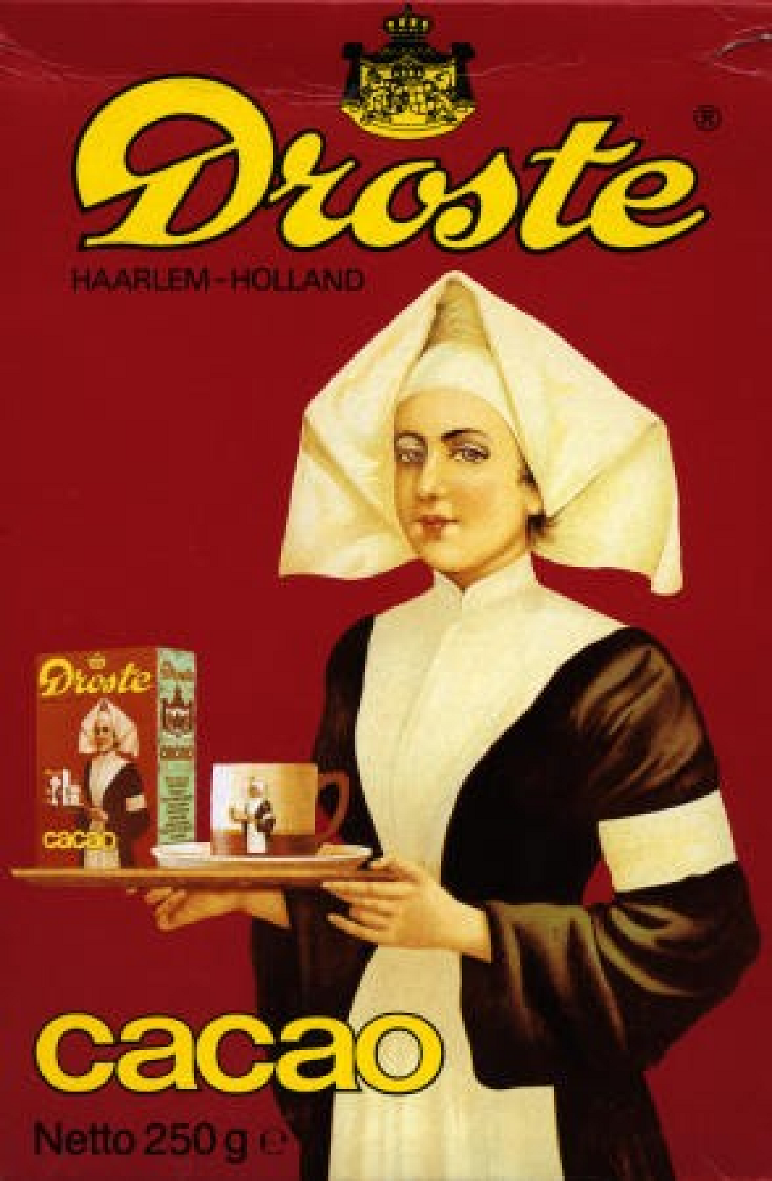
\includegraphics[width=0.38\textwidth]{graficos/droste}
%  \end{center}
%  \caption{\small Una imagen recursiva: la publicidad de Cacao Droste,
%bajada de \url{http://en.wikipedia.org/wiki/Image:Droste.jpg}}
%  \vspace{-3cm}
%\end{wrapfigure}

Estamos acostumbrados a escribir funciones que llaman a otras funciones.
Pero lo cierto es que nada impide que en Python (y en muchos otros
lenguajes) una función se llame a sí misma. Y lo más interesante es que
esta propiedad, que se llama {\it recursión}, permite en muchos casos
encontrar soluciones muy elegantes para determinados problemas. \\

En materias de matemática se estudian los razonamientos por inducción para
probar propiedades de números enteros, la recursión no es más que una
generalización de la inducción a más estructuras: las listas, las cadenas
de caracteres, las funciones, etc.

\begin{figure}
  \begin{center}
    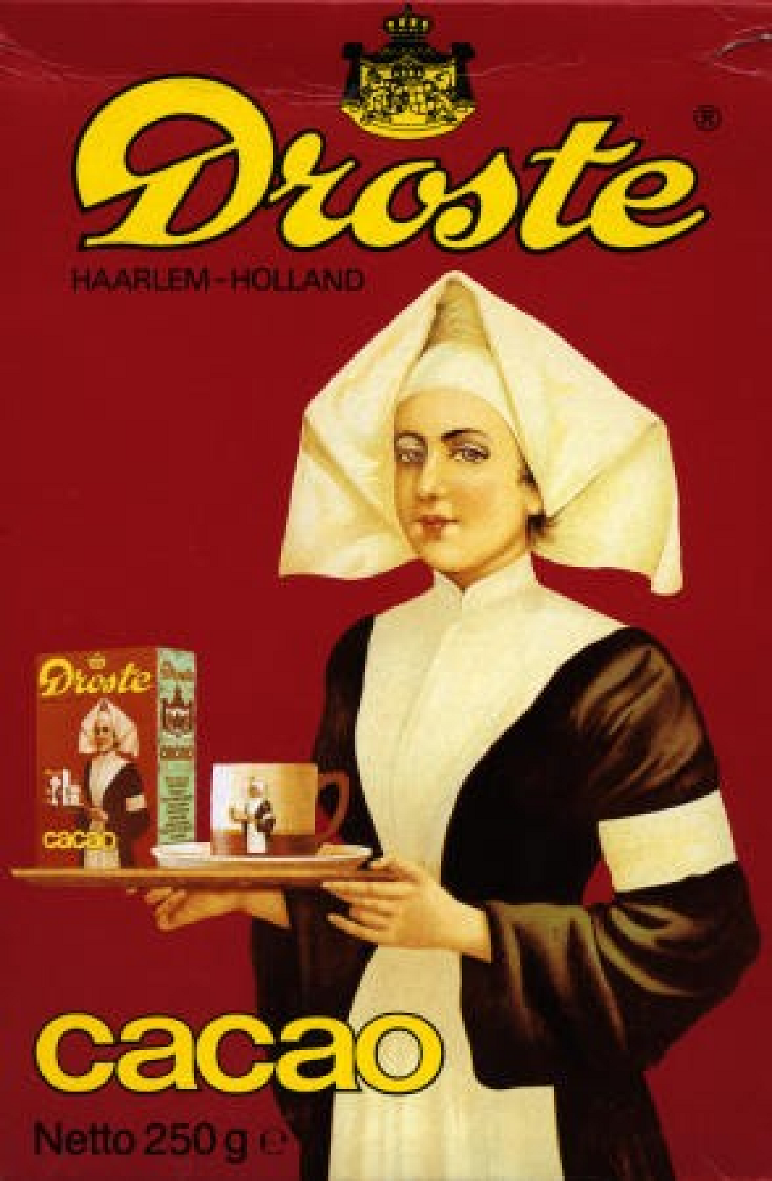
\includegraphics[width=0.38\textwidth]{graficos/droste}
  \end{center}
  \caption{\small Una imagen recursiva: la publicidad de Cacao Droste,
bajada de \url{http://en.wikipedia.org/wiki/Image:Droste.jpg}}
\end{figure}

A continuación estudiaremos diversas situaciones en las cuales aparece la
recursión, veremos cómo es que esto puede funcionar, algunas situaciones en
las que es conveniente utilizarla y otras situaciones en las que no.

% TODO: más que dejar lugar, habría que escribir algo más.
%\vspace{2.5cm}

\section{Una función recursiva matemática}

Es muy común tener definiciones inductivas de operaciones, como por ejemplo:

$x! = x * (x-1)!$ si $x>0$, $0! = 1$

Este tipo de definición se traduce naturalmente en una función en Python:

\begin{codigo-python-sn}
def factorial(n):
    """ Precondición: n entero >=0
        Devuelve: n! """
    if n == 0:
        return 1

    return n * factorial(n-1)
\end{codigo-python-sn}

Esta es la ejecución del factorial para \lstinline!n=0! y para
\lstinline!n=3!.

\begin{codigo-python-sn}
>>> factorial(0)
1
>>> factorial(3)
6
\end{codigo-python-sn}

El sentido de la instrucción de la instrucción
\lstinline|n * factorial (n-1)| es exactamente el mismo que el de la
definición inductiva: para calcular el factorial de $n$ se debe multiplicar
$n$ por el factorial de $n-1$.

Dos piezas fundamentales para garantizar el funcionamiento de este programa
son:

\begin{itemize}
\item Que se defina un {\it caso base} (en este caso la indicación, no recursiva,
de cómo calcular \lstinline|factorial(0)|), que corta las llamadas recursivas.

\item Que el argumento de la función respete la precondición
de que \lstinline!n! debe ser {\it un entero mayor o igual que 0}.
\end{itemize}

Dado que ya vimos la pila de evaluación, y cómo funciona, no debería
llamarnos la atención que esto pueda funcionar adecuadamente en un lenguaje
de programación que utilice pila para evaluar.

Para poder analizar qué sucede a cada paso de la ejecución de la función,
utilizaremos una versión más detallada del mismo código, en la que cada
paso se asigna a una variable.

\begin{codigo-python-sn}
def factorial(n):
    """ Precondición: n entero >=0
        Devuelve: n! """
    if n == 0:
        r = 1
        return r

    f = factorial(n-1)
    r = n * f
    return r
\end{codigo-python-sn}

Esta porción de código funciona exactamente igual que la anterior, pero nos
permite ponerles nombres a los resultados intermedios de cada operación
para poder estudiar qué sucede a cada paso.
Analicemos, entonces, el \lstinline|factorial(3)|  mediante la pila de
evaluación:

\begin{enumerate}

\item  \verb|factorial(3)              |
	\begin{tabular}{r|r|}
	\hline
	\verb|factorial|&n $\rightarrow$3\\
	\hline
	\end{tabular}

\item  \verb|if n == 0:                |
	\begin{tabular}{r|r|}
	\hline
	\verb|factorial|&n $\rightarrow$3\\
	\hline
	\end{tabular}

\item  \verb|f = factorial (n-1)       |
	\begin{tabular}{r|r|}
	\hline
	\verb|factorial|&n $\rightarrow$3\\
	\hline
	\end{tabular}
	\begin{tabular}{l}
	Se suspende el cálculo. \\
	Se llama a \verb|factorial(2)|.
	\end{tabular}

\item  \verb|factorial(2)              |
	\begin{tabular}{r|r|}
	\hline
	\verb|factorial|&n $\rightarrow$2\\
	\hline
	\hline
	\verb|factorial|&n $\rightarrow$3\\
	\hline
	\end{tabular}

\item  \verb|if n == 0:                |
	\begin{tabular}{r|r|}
	\hline
	\verb|factorial|&n $\rightarrow$2\\
	\hline
	\hline
	\verb|factorial|&n $\rightarrow$3\\
	\hline
	\end{tabular}

\item  \verb|f = factorial (n-1)       |
	\begin{tabular}{r|r|}
	\hline
	\verb|factorial|&n $\rightarrow$2\\
	\hline
	\hline
	\verb|factorial|&n $\rightarrow$3\\
	\hline
	\end{tabular}
	\begin{tabular}{l}
	Se suspende el cálculo. \\
	Se llama a \verb|factorial(1)|.
	\end{tabular}

\item  \verb|factorial(1)              |
	\begin{tabular}{r|r|}
	\hline
	\verb|factorial|&n $\rightarrow$1\\
	\hline
	\hline
	\verb|factorial|&n $\rightarrow$2\\
	\hline
	\hline
	\verb|factorial|&n $\rightarrow$3\\
	\hline
	\end{tabular}

\item  \verb|if n == 0:                |
	\begin{tabular}{r|r|}
	\hline
	\verb|factorial|&n $\rightarrow$1\\
	\hline
	\hline
	\verb|factorial|&n $\rightarrow$2\\
	\hline
	\hline
	\verb|factorial|&n $\rightarrow$3\\
	\hline
	\end{tabular}

\item  \verb|f = factorial (n-1)       |
	\begin{tabular}{r|r|}
	\hline
	\verb|factorial|&n $\rightarrow$1\\
	\hline
	\hline
	\verb|factorial|&n $\rightarrow$2\\
	\hline
	\hline
	\verb|factorial|&n $\rightarrow$3\\
	\hline
	\end{tabular}
	\begin{tabular}{l}
	Se suspende el cálculo. \\
	Se llama a \verb|factorial(0)|.
	\end{tabular}

\item  \verb|factorial(0)              |
	\begin{tabular}{r|r|}
	\hline
	\verb|factorial|&n $\rightarrow$0\\
	\hline
	\hline
	\verb|factorial|&n $\rightarrow$1\\
	\hline
	\hline
	\verb|factorial|&n $\rightarrow$2\\
	\hline
	\hline
	\verb|factorial|&n $\rightarrow$3\\
	\hline
	\end{tabular}

\item  \verb|if n == 0:                |
	\begin{tabular}{r|r|}
	\hline
	\verb|factorial|&n $\rightarrow$0\\
	\hline
	\hline
	\verb|factorial|&n $\rightarrow$1\\
	\hline
	\hline
	\verb|factorial|&n $\rightarrow$2\\
	\hline
	\hline
	\verb|factorial|&n $\rightarrow$3\\
	\hline
	\end{tabular}

\item  \verb|r = 1                     |
	\begin{tabular}{r|r|}
	\hline
	\verb|factorial|&n $\rightarrow$0\\
	          &r $\rightarrow$1\\
	\hline
	\hline
	\verb|factorial|&n $\rightarrow$1\\
	\hline
	\hline
	\verb|factorial|&n $\rightarrow$2\\
	\hline
	\hline
	\verb|factorial|&n $\rightarrow$3\\
	\hline
	\end{tabular}

\item
\begin{tabular}{l}
En \lstinline!factorial(0)!: \\ \verb|    return r| \\
En \lstinline!factorial(1)!: \\ \verb|    f = factorial (n-1) |
\end{tabular}
	\begin{tabular}{r|r|}
	\hline
	\verb|factorial|&n $\rightarrow$1\\
	&f $\rightarrow$1\\
	\hline
	\hline
	\verb|factorial|&n $\rightarrow$2\\
	\hline
	\hline
	\verb|factorial|&n $\rightarrow$3\\
	\hline
	\end{tabular}

\item  \verb|r = n * f                 |
\begin{tabular}{r|r|}
\hline
\verb|factorial|&n $\rightarrow$1\\
  &f $\rightarrow$1\\
  &r $\rightarrow$1\\
\hline
\hline
\verb|factorial|&n $\rightarrow$2\\
\hline
\hline
\verb|factorial|&n $\rightarrow$3\\
\hline
\end{tabular}

\item
\begin{tabular}{l}
En \lstinline!factorial(1)!: \\ \verb|    return r| \\
En \lstinline!factorial(2)!: \\ \verb|    f = factorial (n-1) |
\end{tabular}
	\begin{tabular}{r|r|}
	\hline
	\verb|factorial|&n $\rightarrow$2\\
	&f $\rightarrow$1\\
	\hline
	\hline
	\verb|factorial|&n $\rightarrow$3\\
	\hline
	\end{tabular}

\item  \verb|r = n * f                 |
	\begin{tabular}{r|r|}
	\hline
	\verb|factorial|&n $\rightarrow$2\\
	  &f $\rightarrow$1\\
	  &r $\rightarrow$2\\
	\hline
	\hline
	\verb|factorial|&n $\rightarrow$3\\
	\hline
	\end{tabular}

\item
\begin{tabular}{l}
En \lstinline!factorial(2)!: \\ \verb|    return r| \\
En \lstinline!factorial(3)!: \\ \verb|    f = factorial (n-1) |
\end{tabular}
	\begin{tabular}{r|r|}
	\hline
	\verb|factorial|&n $\rightarrow$3\\
	&f $\rightarrow$2\\
	\hline
	\end{tabular}

\item  \verb|r = n * f                 |
	\begin{tabular}{r|r|}
	\hline
	\verb|factorial|&n $\rightarrow$3\\
	  &f $\rightarrow$2\\
	  &r $\rightarrow$6\\
	\hline
	\end{tabular}

\item  \verb|return r                  |
	\begin{tabular}{r|r|}
	\hline
	\verb!    ! pila vacía \verb!   ! \\
	\hline
	\end{tabular}
	\hspace{0.2cm} Devuelve el valor $6$
\end{enumerate}

\begin{minipage}{\linewidth}
\centering%
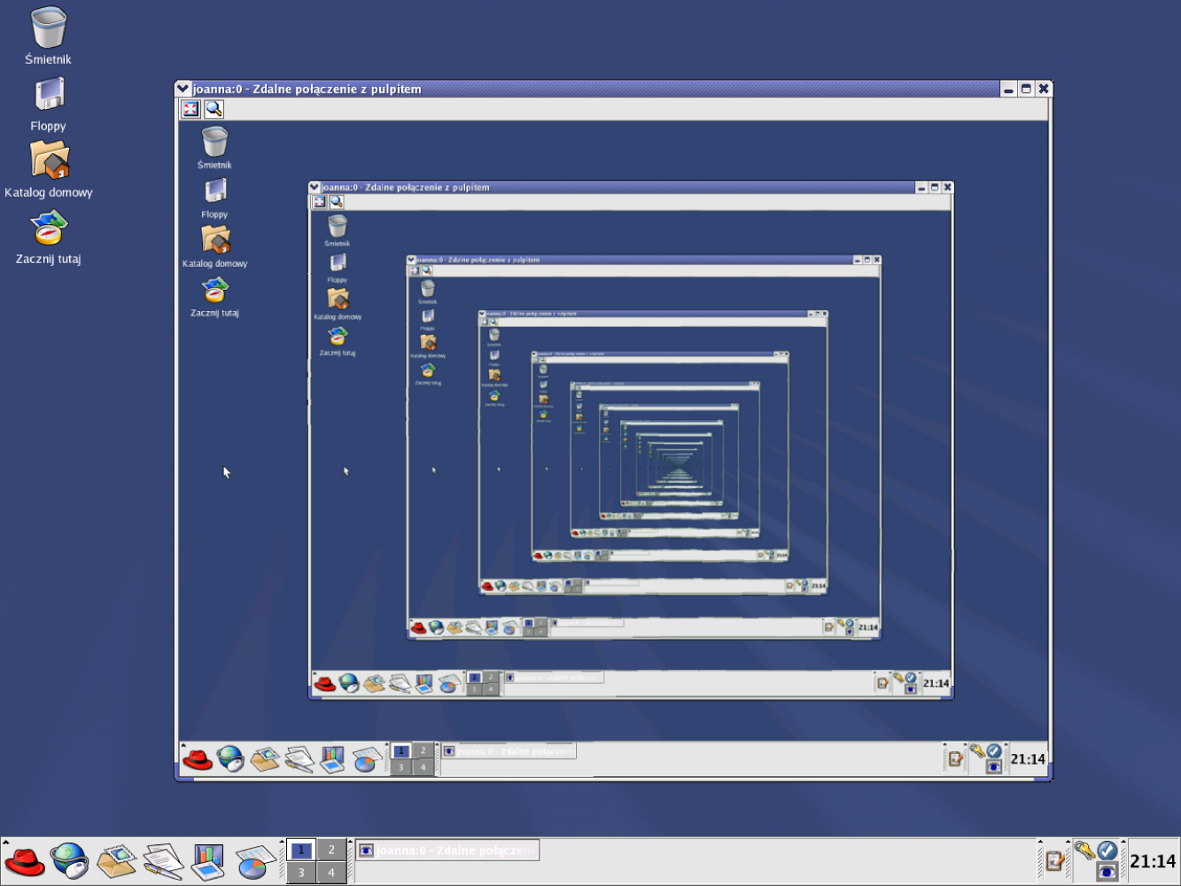
\includegraphics[width=10cm]{graficos/recursive}
\figcaption{Otra imagen recursiva: captura de pantalla de RedHat, bajada de http://www.jfedor.org/}%
\label{fig:redhat_recursivo}%
\end{minipage}

\section{Algoritmos recursivos y algoritmos iterativos}

Llamaremos {\it algoritmos recursivos} a aquellos que realizan llamadas
recursivas para llegar al resultado, y {\it algoritmos iterativos} a
aquellos que llegan a un resultado a través de una iteración mediante un
ciclo definido o indefinido.

Todo algoritmo recursivo puede expresarse como iterativo y viceversa.  Sin
embargo, según las condiciones del problema a resolver podrá ser preferible
utilizar la solución recursiva o la iterativa.

Una posible implementación iterativa de la función \lstinline!factorial!
vista anteriormente sería:

\begin{codigo-python-sn}
def factorial(n):
    """ Precondición: n entero >=0
        Devuelve: n! """

    fact = 1
    for num in xrange(n, 1, -1):
        fact *= num
    return fact
\end{codigo-python-sn}

Se puede ver que en este caso no es necesario incluir un caso base, ya que
el mismo ciclo incluye una condición de corte, pero que sí es necesario
incluir un acumulador, que en el caso recursivo no era necesario.

Por otro lado, si hiciéramos el seguimiento de esta función, como se hizo
para la versión recursiva, veríamos que se trata de una única pila, en la
cual se van modificando los valores de \lstinline!num! y \lstinline!fact!.

Es por esto que las versiones recursivas de los algoritmos, en general,
utilizan más memoria (la pila del estado de las funciones se guarda en
memoria) pero suelen ser más elegantes.

\section{Un ejemplo de recursividad elegante}

Consideremos ahora otro problema que puede ser resuelto de forma elegante
mediante un algoritmo recursivo.

La función \lstinline!potencia(b,n)!, vista en unidades anteriores,
realizaba \lstinline!n! iteraciones para poder obtener el valor de $b^n$.
Sin embargo, es posible optimizarla teniendo en cuenta que: \\

\begin{tabular}{ll}
$b^n = b^{n/2} \times b^{n/2}$ & Si $n$ es par. \\
$b^n = b^{(n-1)/2} \times b^{(n-1)/2} \times b$ &  Si $n$ es impar. \\
\end{tabular} \\

Antes de programar cualquier función recursiva es necesario decidir cuál
será el {\it caso base} y cuál el {\it caso recursivo}.  Para esta función,
tomaremos $n=0$ como el caso base, en el que devolveremos $1$; y el caso
recursivo tendrá dos partes, correspondientes a los dos posibles grupos de
valores de $n$.

\begin{codigo-python-sn}
def potencia(b,n):
    """ Precondición: n debe ser mayor o igual que cero.
        Devuelve: b^n. """

    # Caso base
    if n <= 0:
        return 1

    # n par
    if n % 2 == 0:
        pot = potencia(b, n/2)
        return pot * pot
    # n impar
    else:
        pot = potencia(b, (n-1)/2)
        return pot * pot * b
\end{codigo-python-sn}

El uso de la variable \lstinline!pot! en este caso no es optativo, ya que
es una de las ventajas principales de esta implementación: se aprovecha el
resultado calculado en lugar de tener que calcularlo dos veces. Vemos que
este código funciona correctamente:

\begin{codigo-python-sn}
>>> potencia(2,10)
1024
>>> potencia(3,3)
27
>>> potencia(5,0)
1
\end{codigo-python-sn}

El orden de las llamadas, haciendo un seguimiento simplificado de la
función será:

\begin{enumerate}
\item \verb!potencia(2,10)!
\item \hspace{1cm} \verb!pot = potencia(2,5) !
\hspace{4cm} \begin{tabular}{|c|c|}b $\rightarrow$ 2 & n $\rightarrow$ 10\end{tabular}
\item \hspace{2cm} \verb!pot = potencia(2,2) !
\hspace{3cm} \begin{tabular}{|c|c|}b $\rightarrow$ 2 & n $\rightarrow$ 5$\;\,$\end{tabular}
\item \hspace{3cm} \verb!pot = potencia(2,1) !
\hspace{2cm} \begin{tabular}{|c|c|}b $\rightarrow$ 2 & n $\rightarrow$ 2$\;\,$\end{tabular}
\item \hspace{4cm} \verb!pot = potencia(2,0) !
\hspace{1cm} \begin{tabular}{|c|c|}b $\rightarrow$ 2 & n $\rightarrow$ 1$\;\,$\end{tabular}
\item \hspace{5cm} \verb!return 1            !
\hspace{0cm} \begin{tabular}{|c|c|}b $\rightarrow$ 2 & n $\rightarrow$ 0$\;\,$\end{tabular}
\item \hspace{4cm} \verb!return 1 * 1 * 2    !
\hspace{1cm} \begin{tabular}{|c|c|c|}b $\rightarrow$ 2 & n $\rightarrow$ 1$\;\,$
& pot $\rightarrow$ 1$\;\,$ \end{tabular}
\item \hspace{3cm} \verb!return 2 * 2        !
\hspace{2cm} \begin{tabular}{|c|c|c|}b $\rightarrow$ 2 & n $\rightarrow$ 2$\;\,$
& pot $\rightarrow$ 2$\;\,$ \end{tabular}
\item \hspace{2cm} \verb!return 4 * 4 * 2    !
\hspace{3cm} \begin{tabular}{|c|c|c|}b $\rightarrow$ 2 & n $\rightarrow$ 5$\;\,$
& pot $\rightarrow$ 4$\;\,$ \end{tabular}
\item \hspace{1cm} \verb!return 32 * 32      !
\hspace{4cm} \begin{tabular}{|c|c|c|}b $\rightarrow$ 2 & n $\rightarrow$ 10
& pot $\rightarrow$ 32 \end{tabular}
\end{enumerate}

Se puede ver, entonces, que para calcular $2^{10}$ se realizaron 5 llamadas a
\lstinline!potencia!, mientras que en la implementación más sencilla se
realizaban 10 iteraciones. Y esta optimización será cada vez más importante
a medida que aumenta \lstinline!n!, por ejemplo, para $n = 100$ se
realizarán 8 llamadas recursivas, para $n = 1000$, 11 llamadas. \\

% Esto no es para darlo, es sólo para que esté

Para transformar este algoritmo recursivo en un algoritmo iterativo, es
necesario {\it simular} la pila de llamadas a funciones mediante una pila que
almacene los valores que sean necesarios.  En este caso, lo que apilaremos será
si el valor de \lstinline!n! es par o no.

\begin{codigo-python-sn}
def potencia(b,n):
    """ Precondición: n debe ser mayor o igual que cero.
        Devuelve: b^n. """

    pila = []
    while n > 0:
        if n % 2 == 0:
            pila.append(True)
            n /= 2
        else:
            pila.append(False)
            n = (n-1)/2

    pot = 1
    while pila:
        es_par = pila.pop()
        if es_par:
            pot = pot * pot
        else:
            pot = pot * pot * b

    return pot
\end{codigo-python-sn}

Como se puede ver, este código es mucho más complejo que la versión recursiva,
esto se debe a que utilizando recursividad el uso de la pila de llamadas a
funciones oculta el proceso de apilado y desapilado y permite concentrarse
en la parte importante del algoritmo.

\section{Un ejemplo de recursividad poco eficiente}

Del ejemplo anterior se podría deducir que siempre es mejor utilizar algoritmos
recursivos, sin embargo -como ya se dijo- cada situación debe ser analizada por
separado.

Un ejemplo clásico en el cual la recursividad tiene un resultado muy poco
eficiente es el de los números de fibonacci.  La sucesión de fibonacci está
definida por la siguiente relación:

\begin{tabular}{rcl}
\lstinline!fib(0)! &=& 0 \\
\lstinline!fib(1)! &=& 1 \\
\lstinline!fib(n)! &=& \lstinline!fib(n-1)! + \lstinline!fib(n-2)!
\end{tabular}

Los primeros números de esta sucesión son: $0$, $1$, $1$, $2$, $3$, $5$, $8$,
$13$, $21$, $34$, $55$.

Dada la definición recursiva de la sucesión, puede resultar muy tentador
escribir una función que calcule en valor de \lstinline!fib(n)! de la siguiente
forma:

\begin{codigo-python-sn}
def fib(n):
    """ Precondición: n debe ser >= 0.
        Devuelve: el número de fibonacci número n. """
    if n == 0 or n == 1:
        return n
    return fib(n-1) + fib(n-2)
\end{codigo-python-sn}

Sin embargo, si bien es muy sencillo y elegante, este código es extremadamente
poco eficiente.  Ya que para calcular \lstinline!fib(n-1)! es necesario calcular
\lstinline!fib(n-2)!, que luego volverá a ser calculado para obtener el valor de
\lstinline!fib(n)!.

Por ejemplo, una simple llamada a \lstinline!fib(5)!, generaría
recursivamente todas las llamadas ilustradas en la Figura \ref{fibonacci}.
Puede verse que muchas de estas llamadas están repetidas, generando un
total de 15 llamadas a la función \lstinline!fib!, sólo para devolver el
número 5.

\begin{figure}[htb]
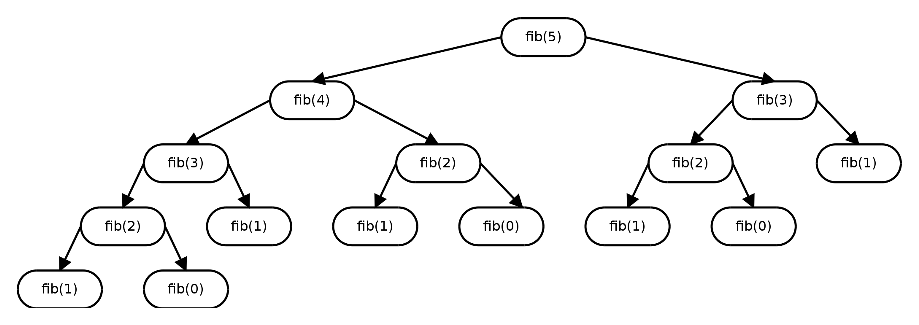
\includegraphics{graficos/18_fibonacci}
\caption{Árbol de llamadas para \lstinline!fib(5)!}
\label{fibonacci}
\end{figure}

En este caso, será mucho más conveniente utilizar una versión iterativa,
que vaya almacenando los valores de las dos variables anteriores a medida
que los va calculando.

% FIXME: hace falta un newpage, porque sino corta el código mal
\newpage

\begin{codigo-python-sn}
def fib(n):
    """ Precondición: n debe ser >= 0.
        Devuelve: el número de fibonacci número n. """
    if n == 0 or n == 1:
        return n

    ant2 = 0
    ant1 = 1
    for i in xrange(2, n+1):
        fibn = ant1 + ant2
        ant2 = ant1
        ant1 = fibn
    return fibn
\end{codigo-python-sn}

Vemos que el caso base es el mismo para ambos algoritmos, pero que en el
caso iterativo se calcula el número de fibonacci de forma incremental, de
modo que para obtener el valor de \lstinline!fib(n)! se harán $n-1$
iteraciones.

\begin{atencion}
En definitiva, vemos que un algoritmo recursivo {\bf no} es mejor que uno
iterativo, ni viceversa.  En cada situación será conveniente analizar cuál
algoritmo provee la solución al problema de forma más clara y eficiente.
\end{atencion}

\section{Limitaciones}

Si creamos una función sin {\it caso base}, obtendremos el equivalente
recursivo de un bucle infinito.  Sin embargo, como cada llamada recursiva
agrega un elemento a la pila de llamadas a funciones y la memoria de
nuestras computadoras no es infinita, el ciclo deberá terminarse cuando se
agote la memoria disponible.

En particular, en Python, para evitar que la memoria se termine, la pila de
ejecución de funciones tiene un límite. Es decir, que si se ejecuta un
código como el que sigue:

\begin{codigo-python-sn}
def inutil(n):
    return inutil(n-1)
\end{codigo-python-sn}

Se obtendrá un resultado como el siguiente:

\begin{codigo-python-sn}
>>> inutil(1)
  File "<stdin>", line 2, in inutil
  File "<stdin>", line 2, in inutil
  (...)
  File "<stdin>", line 2, in inutil
RuntimeError: maximum recursion depth exceeded
\end{codigo-python-sn}

El límite por omisión es de 1000 llamadas recursivas. Es posible modificar
el tamaño máximo de la pila de recursión mediante la instrucción
\lstinline!sys.setrecursionlimit(n)!.  Sin embargo, si se está alcanzando
este límite suele ser una buena idea pensar si realmente el algoritmo
recursivo es el que mejor resuelve el problema.

\begin{sabias_que}
Existen algunos lenguajes {\it funcionales}, como Haskell, ML, o Scheme, en
los cuales la recursividad es la única forma de realizar un ciclo.  Es
decir, no existen construcciones {\tt while} ni {\tt for}.

Estos lenguajes cuentan con una optimización especial, llamada {\it
optimización de recursión por cola} ({\it tail recursion optimization}),
que permite que cuando una función realiza su llamada recursiva como {\bf
última} acción antes de terminar, no se apile el estado de la función
innecesariamente, evitando el consumo adicional de memoria mencionado
anteriormente.

La función \lstinline!factorial! vista en esta unidad es un ejemplo de {\it
recursión por cola} cuya ejecución puede ser optimizada por el compilador o
intérprete del lenguaje.
\end{sabias_que}

\section{Resumen}

\begin{itemize}

\item A medida que se realizan llamadas a funciones, el estado de las
funciones anteriores se almacena en una {\it pila} de llamadas a funciones.

\item Esto permite que sea posible que una función se llame a sí misma,
pero que las variables dentro de la función tomen distintos valores.

\item La {\bf recursión} es el proceso en el cual una función se llama a
sí misma.  Este proceso permite crear un nuevo tipo de ciclos.

\item Siempre que se escribe una función recursiva es importante considerar
el {\bf caso base} (el que detendrá la recursividad) y el {\bf caso
recursivo} (el que realizará la llamada recursiva).  Una función recursiva
sin caso base, es equivalente a un bucle infinito.

\item Una función no es mejor ni peor por ser recursiva.  En cada situación
a resolver puede ser conveniente utilizar una solución recursiva o una
iterativa.  Para elegir una o la otra será necesario analizar las
características de elegancia y eficiencia.

\end{itemize}


\newpage
\section{Ejercicios}

\extractionlabel{guia}
\begin{ejercicio}
Escribir una función que reciba un número positivo $n$ y devuelva
la cantidad de dígitos que tiene.
\end{ejercicio}

\extractionlabel{guia}
\begin{ejercicio}
Escribir una función que simule el siguiente experimento:
Se tiene una rata en una jaula con 3 caminos, entre los cuales elige
al azar (cada uno tiene la misma probabilidad), si elige el {\it 1} luego
de 3 minutos vuelve a la jaula, si elige el {\it 2} luego de 5 minutos vuelve a
la jaula, en el caso de elegir el {\it 3} luego de 7 minutos sale de la jaula.
La rata no aprende, siempre elige entre los 3 caminos con la misma probabilidad,
pero quiere su libertad, por lo que recorrerá los caminos hasta salir de la jaula.

La función debe devolver el tiempo que tarda la rata en salir de la jaula.
\end{ejercicio}

\extractionlabel{guia}
\begin{ejercicio}
Escribir una función que reciba 2 enteros {\it n} y {\it b} y devuelva
\verb!True! si {\it n} es potencia de {\it b}.

Ejemplos:
\begin{verbatim}
>>> es_potencia(8,2)
True
>>> es_potencia(64,4)
True
>>> es_potencia(70,10)
False
\end{verbatim}
\end{ejercicio}

\extractionlabel{guia}
\begin{ejercicio}
Escribir una funcion recursiva que reciba como parámetros dos strings {\it a} y
{\it b}, y devuelva una lista con las posiciones en donde se encuentra {\it b}
dentro de {\it a}.

Ejemplo:
\begin{verbatim}
>>> posiciones_de("Un tete a tete con Tete", "te")
[3, 5, 10, 12, 21]
\end{verbatim}
\end{ejercicio}

\extractionlabel{guia}
\begin{ejercicio}
Escribir dos funciones mutualmente recursivas par(n) e impar(n) que
determinen la paridad del numero natural dado, conociendo solo que:
\begin{itemize}
    \item 1 es impar.
    \item Si un número es impar, su antecesor es par; y viceversa.
\end{itemize}
\end{ejercicio}

\extractionlabel{guia}
\begin{ejercicio}
Escribir una función que calcule recursivamente el n-ésimo número
triangular (el número 1 + 2 + 3 + ... + n).
\end{ejercicio}

\extractionlabel{guia}
\begin{ejercicio}
Escribir una función que calcule recursivamente cuántos elementos
hay en una pila, suponiendo que la pila sólo tiene los métodos apilar
y desapilar, y no altere el contenido de la pila.\\
¿Implementarías esta función para un programa real? ¿Por qué?
\end{ejercicio}

\extractionlabel{guia}
\begin{ejercicio}
Escribir una funcion recursiva que encuentre el mayor elemento de una lista.
\end{ejercicio}

\extractionlabel{guia}
\begin{ejercicio}
Escribir una función recursiva para replicar los elementos de una lista
una cantidad n de veces. Por ejemplo,
\verb!replicar ([1, 3, 3, 7], 2) = ([1, 1, 3, 3, 3, 3, 7, 7])!
\end{ejercicio}


% Copyright (C) 2008-2010 Rosita Wachenchauzer <rositaw@gmail.com>
%               Margarita Manterola <margamanterola@gmail.com>

% Esta obra está licenciada de forma dual, bajo las licencias Creative
% Commons:
%  * Atribución-Compartir Obras Derivadas Igual 2.5 Argentina
%    http://creativecommons.org/licenses/by-sa/2.5/ar/
%  * Atribución-Compartir Obras Derivadas Igual 3.0 Unported
%    http://creativecommons.org/licenses/by-sa/3.0/deed.es_AR.
%
% A su criterio, puede utilizar una u otra licencia, o las dos.
% Para ver una copia de las licencias, puede visitar los sitios
% mencionados, o enviar una carta a Creative Commons,
% 171 Second Street, Suite 300, San Francisco, California, 94105, USA.

\chapter{Ordenar listas}

Al estudiar las listas de Python, vimos que poseen un método \lstinline!sort!
que las ordena de menor a mayor de acuerdo a una clave (e incluso de acuerdo a
una relación de orden que se desee, dada a través del parámetro
\lstinline!cmp!).

Sin embargo, no todas las estructuras cuentan con un método
\lstinline!sort! que las ordene.  Es por ello que en esta unidad nos
plantearemos cómo se hace para ordenar cuando no hay un método
\lstinline!sort!, y cuánto cuesta ordenar.

Ante todo una advertencia: hay varias maneras de ordenar, y no todas
cuestan lo mismo. Vamos a empezar viendo las más sencillas de escribir
(que en general suelen ser las más caras).

\section{Ordenamiento por selección}
Éste método de ordenamiento se basa en la siguiente idea:

\begin{itemize}

\item {\bf Paso 1.1}: Buscar el mayor de todos los elementos de la lista.
\\

\hspace{0.75cm}
\begin{tabular}[c]{|c|c|c|c|c|c|}
\hline
3& 2&-1&5&0&2\\
\hline
\end{tabular}
\hspace{0.75cm}
\begin{tabular}{p{9cm}}
Encuentra el valor $5$ en la posición $3$.
\end{tabular}\\

\item {\bf Paso 1.2}: Poner el mayor al final (intercambiar el que está en la última
posición de la lista con el mayor encontrado).\\

\hspace{0.75cm}
\begin{tabular}[c]{|c|c|c|c|c|c|}
\hline
3& 2&-1&2&0&5\\
\hline
\end{tabular}
\hspace{0.75cm}
\begin{tabular}{p{9cm}}
Intercambia el elemento de la posición $3$ con el de la posición $5$. \\
{\it En la última posición de la lista está el mayor de todos.}
\end{tabular} \\

\item {\bf Paso 2.1}: Buscar el mayor de todos los elementos del segmento de la lista
entre la primera y la anteúltima posición. \\

\hspace{0.75cm}
\begin{tabular}[c]{|c|c|c|c|c|c|}
\hline
3& 2&-1&2&0&5\\
\hline
\end{tabular}
\hspace{0.75cm}
\begin{tabular}{p{9cm}}
Encuentra el valor $3$ en la posición $0$.
\end{tabular} \\

\item {\bf Paso 2.2}: Poner el mayor al final del segmento (intercambiar el que está en la última
posición del segmento --o sea anteúltima posición de la lista-- con el mayor encontrado). \\

\hspace{0.75cm}
\begin{tabular}[c]{|c|c|c|c|c|c|}
\hline
0& 2&-1&2&3&5\\
\hline
\end{tabular}
\hspace{0.75cm}
\begin{tabular}{p{9cm}}
Intercambia el elemento de la posición $0$ con el valor de la posición $4$. \\
{\it En la anteúltima y última posición de la lista están los dos mayores en su posición definitiva.}
\end{tabular} \\

$\dots$\\

\item {\bf Paso n}: Se termina cuando queda un único elemento sin tratar: el que está
en la primera posición de la lista, y que es el menor de todos porque todos los
mayores fueron reubicados. \\

\hspace{0.75cm}
\begin{tabular}[c]{|c|c|c|c|c|c|}
\hline
-1& 0&2&2&3&5\\
\hline
\end{tabular}
\hspace{0.75cm}
\begin{tabular}{p{9cm}}
{\it La lista se encuentra ordenada}.
\end{tabular}\\
\end{itemize}

\begin{codigo}{seleccion.py}{Ordena una lista por selección}
\label{ord_seleccion}
\lstinputlisting{src/19_ordenamiento/seleccion.py}
\end{codigo}

La implementación en Python puede verse en el Código \ref{ord_seleccion}.


La función principal, \lstinline!ord_seleccion! es la encargada de recorrer
la lista, ubicando el mayor elemento al final del segmento y luego
reduciendo el segmento a analizar.

Mientras que \lstinline!buscar_max! es una función que ya se estudió
previamente, que busca el mayor elemento de la lista y devuelve su
posición.

A continuación, algunas una ejecuciones de prueba de ese código:

\begin{codigo-python-sn}
>>> l=[3, 2, -1, 5, 0, 2]
>>> ord_seleccion(l)
DEBUG:  3 5 [3, 2, -1, 2, 0, 5]
DEBUG:  0 4 [0, 2, -1, 2, 3, 5]
DEBUG:  1 3 [0, 2, -1, 2, 3, 5]
DEBUG:  1 2 [0, -1, 2, 2, 3, 5]
DEBUG:  0 1 [-1, 0, 2, 2, 3, 5]
>>> print l
[-1, 0, 2, 2, 3, 5]
>>> l=[]
>>> ord_seleccion(l)
>>> l=[1]
>>> ord_seleccion(l)
>>> print l
[1]
>>> l=[1,2,3,4,5]
>>> ord_seleccion(l)
DEBUG:  4 4 [1, 2, 3, 4, 5]
DEBUG:  3 3 [1, 2, 3, 4, 5]
DEBUG:  2 2 [1, 2, 3, 4, 5]
DEBUG:  1 1 [1, 2, 3, 4, 5]
\end{codigo-python-sn}

Puede verse que aún cuando la lista está ordenada, se la recorre buscando
los mayores elementos y ubicándolos en la misma posición en la que se
encuentran.

\subsection{Invariante en el ordenamiento por selección}

Todo ordenamiento tiene un invariante que permite asegurarse de que cada
paso que se toma va en la dirección de obtener una lista ordenada.

En el caso del ordenamiento por selección, el invariante es que los
elementos desde \lstinline!n+1! hasta el final de la lista están ordenados y
son mayores que los elementos de \lstinline!0! a \lstinline!n!, es decir
que ya están en su posición definitiva.

\subsection{¿Cuánto cuesta ordenar por selección?}

Como se puede ver en el código de la función \lstinline!buscar_max!, para
buscar el máximo elemento en un segmento de lista se debe recorrer todo ese
segmento, por lo que en nuestro caso debemos recorrer en el primer paso $N$
elementos, en el segundo paso $N-1$ elementos, en el tercer paso $N-2$
elementos, etc. Cada visita a un elemento implica una cantidad constante y
pequeña de comparaciones (que no depende de $N$). Por lo tanto tenemos que

\begin{equation}
T(N) \approx c * (2 + 3 + \ldots + N) \approx c * N * (N+1)/2 \sim N^2
\end{equation}

O sea que ordenar por selección una lista de tamaño $N$ insume tiempo del
orden de $N^2$.  Como ya se vio, este tiempo es independiente de si la
lista estaba previamente ordenda o no.

En cuanto al espacio utilizado, sólo se tiene en memoria la
lista que se desea ordenar y algunas variables de tamaño 1.

\section{Ordenamiento por inserción}

Éste otro método de ordenamiento se basa en la siguiente idea:

\begin{itemize}

\item {\bf Paso 0}: Partimos de la misma lista de ejemplo utilizada para el ordenamiento
por selección. \\

\hspace{0.75cm}
\begin{tabular}[c]{|c|c|c|c|c|c|}
\hline
3& 2&-1&5&0&2\\
\hline
\end{tabular}
\hspace{0.75cm}

\item {\bf Paso 1}: Considerar el segundo elemento de la lista,
y ordenarlo respecto del primero, deplazándolo hasta la
posición correcta, si corresponde. \\

\hspace{0.75cm}
\begin{tabular}[c]{|c|c|c|c|c|c|}
\hline
2& 3&-1&5&0&2\\
\hline
\end{tabular}
\hspace{0.75cm}
\begin{tabular}{p{9cm}}
Se desplaza el valor $2$ antes de $3$.
\end{tabular}

\item {\bf Paso 2}: Considerar el tercer elemento de la lista,
y ordenarlo respecto del primero y el segundo, deplazándolo hasta la
posición correcta, si corresponde. \\

\hspace{0.75cm}
\begin{tabular}[c]{|c|c|c|c|c|c|}
\hline
-1& 2&3&5&0&2\\
\hline
\end{tabular}
\hspace{0.75cm}
\begin{tabular}{p{9cm}}
Se desplaza el valor $-1$ antes de $2$ y de $3$.
\end{tabular}

\item {\bf Paso 3}: Considerar el cuarto elemento de la lista,
y ordenarlo respecto del primero, el segundo y el tercero, deplazándolo hasta la
posición correcta, si corresponde. \\

\hspace{0.75cm}
\begin{tabular}[c]{|c|c|c|c|c|c|}
\hline
-1& 2&3&5&0&2\\
\hline
\end{tabular}
\hspace{0.75cm}
\begin{tabular}{p{9cm}}
El $5$ está correctamente ubicado respecto de $-1$,$2$ y $3$ (como el segmento
hasta la tercera posición está ordenado, basta con comparar con el tercer elemento del
segmento para verificarlo).\\
\end{tabular}

$\dots$\\

\item {\bf Paso N-1}: \\

\hspace{0.75cm}
\begin{tabular}[c]{|c|c|c|c|c|c|}
\hline
-1& 0&2&3&5&2\\
\hline
\end{tabular}
\hspace{0.75cm}
\begin{tabular}{p{9cm}}
Todos los elementos excepto el ante-último ya se encuentran ordenados.
\end{tabular}

\item {\bf Paso N}:
Considerar el $N$--ésimo elemento de la lista, y ordenarlo respecto del
segmento formado por el primero hasta el $N-1$--ésimo, deplazándolo hasta
la posición correcta, si corresponde. \\

\hspace{0.75cm}
\begin{tabular}[c]{|c|c|c|c|c|c|}
\hline
-1& 0&2&2&3&5\\
\hline
\end{tabular}
\hspace{0.75cm}
\begin{tabular}{p{9cm}}
Se desplaza el valor $2$ antes de $3$ y de $5$.
\end{tabular}

\end{itemize}

\begin{codigo}{insercion.py}{Ordena una lista por Inserción}
\label{ord_insercion}
\lstinputlisting{src/19_ordenamiento/insercion.py}
\end{codigo}

Una posible implementación en Python de este algoritmo se incluye en el
Código \ref{ord_insercion}.

La función principal, \lstinline!ord_insercion!, recorre la lista desde el
segundo elemento hasta el último, y cuando uno de estos elementos no está
ordenado con respecto al anterior, llama a la función auxiliar
\lstinline!reubicar!, que se encarga de colocar el elemento en la posición
que le corresponde.

En la función \lstinline!reubicar! se busca la posición correcta donde debe
colocarse el elemento, a la vez que se van corriendo todos los elementos un
lugar a la derecha, de modo que cuando se encuentra la posición, el valor a
insertar reemplaza al valor que se encontraba allí anteriormente.

En las siguientes ejecuciones puede verse que funciona correctamente.

\begin{codigo-python-sn}
>>> l=[3, 2,-1,5, 0, 2]
>>> ord_insercion(l)
DEBUG:  [2, 3, -1, 5, 0, 2]
DEBUG:  [-1, 2, 3, 5, 0, 2]
DEBUG:  [-1, 2, 3, 5, 0, 2]
DEBUG:  [-1, 0, 2, 3, 5, 2]
DEBUG:  [-1, 0, 2, 2, 3, 5]
>>> print l
[-1, 0, 2, 2, 3, 5]
>>> l=[]
>>> ord_insercion(l)
>>> l=[1]
>>> ord_insercion(l)
>>> print l
[1]
>>> l=[1,2,3,4,5,6]
>>> ord_insercion(l)
DEBUG:  [1, 2, 3, 4, 5, 6]
DEBUG:  [1, 2, 3, 4, 5, 6]
DEBUG:  [1, 2, 3, 4, 5, 6]
DEBUG:  [1, 2, 3, 4, 5, 6]
DEBUG:  [1, 2, 3, 4, 5, 6]
>>> print l
[1, 2, 3, 4, 5, 6]
\end{codigo-python-sn}

\subsection{Invariante del ordenamiento por inserción}

En el ordenamiento por inserción, a cada paso se considera que los
elementos que se encuentran en el segmento de $0$ a $i$ están ordenados, de
manera que agregar un nuevo elemento implica colocarlo en la posición
correspondiente y el segmento seguirá ordenado.

\subsection{¿Cuánto cuesta ordenar por inserción?}

Del Código \ref{ord_insercion} se puede ver que la función principal avanza por la
lista de izquierda a derecha, mientras que la función \lstinline!reubicar!
cambia los elementos de lugar de derecha a izquierda.

Lo peor que le puede pasar a un elemento que está en la posición
$j$ es que deba ser ubicado al principio de la lista.  Y lo peor que le
puede pasar a una lista es que todos sus elementos deban ser reubicados.

Por ejemplo, en la lista \lstinline+[10, 8, 6, 2, -2, -5]+, todos los
elementos deben ser reubicados al principio de la lista.

En el primer paso, el segundo elemento se debe intercambiar con el primero;
en el segundo paso, el tercer elemento se compara con el segundo y el
primer elemento, y se ubica adelante de todo; en el tercer paso, el cuarto
elemento se compara con el tercero, el segundo y el primer elemento, y se
ubica adelante de todo; etc...

\begin{equation}
T(N) \approx c * (2 + 3 + \ldots + N) \approx c * N * (N+1)/2 \sim N^2
\end{equation}

Es decir que ordenar por inserción una lista de tamaño $N$ puede insumir
(en el peor caso) tiempo del orden de $N^2$. En cuanto al espacio
utilizado, nuevamente sólo se tiene en memoria la lista que se desea
ordenar y algunas variables de tamaño 1.

\subsection{Inserción en una lista ordenada}

Sin embargo, algo interesante a notar es que cuando la lista se encuentra
ordenada, este algoritmo no hace ningún movimiento de elementos,
simplemente compara cada elemento con el anterior, y si es mayor sigue
adelante.

Es decir que para el caso de una lista de $N$ elementos que se encuentra
ordenada, el tiempo que insume el algoritmo de inserción es:

\begin{equation}
T(N) \sim N
\end{equation}

% TODO: burbujeo

\section{Resumen}

\begin{itemize}

\item El ordenamiento por selección, es uno de los más sencillos, pero es
bastante ineficiente, se basa en la idea de buscar el máximo en una secuencia,
ubicarlo al final y seguir analizando la secuencia sin el último elemento.
Tiene como ventaja que hace una baja cantidad de ``intercambios'' ($N$), pero
como desventaja que necesita una alta cantidad de comparaciones ($N^2$).
Siempre tiene el mismo comportamiento.

\item El ordenamiento por inserción, es un algoritmo bastante intuitivo y se
suele usar para ordenar en la vida real. Se basa en la idea de ir insertando
ordenadamente, en cada paso se considera la inserción de un elemento más de
secuencia y la inserción se empieza a hacer desde el final de los datos ya
ordenados.

Tiene como ventaja que en el caso de tener los datos ya ordenados no hace
ningún intercambio (y hace sólo $N-1$ comparaciones). En el peor caso, cuando
la secuencia está invertida, se hace una gran cantidad de intercambios y
comparaciones ($N^2$). Si bien es un algoritmo ineficiente, para secuencias
cortas, el tiempo de ejecución es bastante bueno.

%\item Burbujeo
\end{itemize}

\newpage
\section{Ejercicios}

\extractionlabel{guia}
\begin{ejercicio}
Implementar una función que reciba una lista y devuelva otra lista con los
mismos elementos que la primera, ordenados de mayor a menor mediante el método
de inserción.
\end{ejercicio}

% Copyright (C) 2008-2010 Rosita Wachenchauzer <rositaw@gmail.com>
%               Margarita Manterola <margamanterola@gmail.com>

% Esta obra est� licenciada de forma dual, bajo las licencias Creative
% Commons:
%  * Atribuci�n-Compartir Obras Derivadas Igual 2.5 Argentina
%    http://creativecommons.org/licenses/by-sa/2.5/ar/
%  * Atribuci�n-Compartir Obras Derivadas Igual 3.0 Unported
%    http://creativecommons.org/licenses/by-sa/3.0/deed.es_AR.
%
% A su criterio, puede utilizar una u otra licencia, o las dos.
% Para ver una copia de las licencias, puede visitar los sitios
% mencionados, o enviar una carta a Creative Commons,
% 171 Second Street, Suite 300, San Francisco, California, 94105, USA.

\chapter{Algunos ordenamientos recursivos}

Los m�todos de ordenamiento vistos en la unidad anterior eran m�todos
iterativos cuyo tiempo estaba relacionado con $N^2$.

En esta unidad veremos dos m�todos de ordenamiento, basados
�stos en un planteo recursivo del problema, que nos permitir�n obtener el
mismo resultado de forma m�s eficiente.

\section{Ordenamiento por mezcla, o {\it Merge sort} }

Este m�todo se basa en la siguiente idea:
\begin{enumerate}
\item Si la lista es peque�a (vac�a o de tama�o 1) ya est� ordenada y
no hay nada que hacer. De lo contrario hacer lo siguiente:
\item Dividir la lista al medio, formando dos sublistas de (aproximadamente) el
mismo tama�o cada una.
\item Ordenar cada una de esas dos sublistas (usando
este mismo m�todo).
\item Una vez que se ordenaron ambas sublistas, intercalarlas de manera ordenada.
\end{enumerate}

Por ejemplo, si la lista original es \lstinline+[6, 7, -1, 0, 5, 2, 3, 8]+
deberemos ordenar recursivamente \lstinline+[6, 7, -1, 0]+ y 
\lstinline+[5, 2, 3, 8]+ con lo cual obtendremos \lstinline+[-1, 0, 6, 7]+ y
\lstinline+[2, 3, 5, 8]+.  Si intercalamos ordenadamente las dos listas
ordenadas obtenemos la soluci�n buscada: 
\lstinline+[-1, 0, 2, 3, 5, 6, 7, 8]+.

Dise�amos la {\bf funci�n \lstinline!merge_sort(lista)!}:

\begin{enumerate}
\item Si lista es peque�a (vac�a o de tama�o 1) ya est� ordenada y
no hay nada que hacer. Se devuelve lista tal cual.
\item De lo contrario:
\begin{enumerate}
\item medio = len(lista)/2
\item izq = merge\_sort(lista[:m])
\item der = merge\_sort(lista[m:])
\item Se devuelve merge(izq, der).
\end{enumerate}
\end{enumerate}

Falta s�lo dise�ar la funci�n \lstinline!merge! que realiza la
intercalaci�n ordenada de dos listas ordenadas (dadas dos listas ordenadas
se debe obtener una nueva lista que resulte de intercalar a ambas de manera
ordenada).

Dise�amos la {\bf funci�n \lstinline!merge(lista1, lista2)!}:

\begin{enumerate}
\item Utilizaremos dos �ndices, \lstinline!i! y \lstinline!j!, para recorrer
cada una de las dos listas.
\item Utilizaremos una tercera lista, \lstinline!resultado!, donde
almacenaremos el resultado.

\item Mientras \lstinline!i! sea menor que el largo de \lstinline!lista1! y
\lstinline!j! menor que el largo de \lstinline!lista2!, significa que hay
elementos para comparar en ambas listas.

\begin{enumerate}
\item Si el menor es el de \lstinline!lista1!:
\begin{enumerate}
\item Agregar el elemento \lstinline!i! de \lstinline!lista1! al final del
resultado.  
\item Avanzar el �ndice \lstinline!i!.
\end{enumerate}
\item de lo contrario:
\begin{enumerate}
\item Agregar el elemento \lstinline!j! de \lstinline!lista2! al final del
resultado.
\item Avanzar el �ndice \lstinline!j!.
\end{enumerate}

\end{enumerate}

\item Una vez que una de las dos listas se termina, simplemente hay que
agregar todo lo que queda en la otra al final del resultado.
\end{enumerate}

\begin{codigo}{mergesort.py}{Una implementaci�n de {\it Merge sort}}
\lstinputlisting{src/20_ordenamiento_recursivo/mergesort.py}
\label{src:mergesort}
\end{codigo}	

El c�digo resultante del dise�o de ambas funciones puede verse en el C�digo
\ref{src:mergesort}. 

\begin{sabias_que}
El m�todo que hemos usado para resolver este problema se llama {\bf Divisi�n y
Conquista}, y se aplica en las situaciones en las que vale el siguiente
principio:

Para obtener una soluci�n es posible partir el problema en varios subproblemas
de tama�o menor, resolver cada uno de esos subproblemas por separado aplicando
la misma t�cnica (en nuestro caso ordenar por mezcla cada una de las dos
sublistas), y finalmente juntar estas soluciones parciales en una soluci�n
completa del problema mayor (en nuestro caso la intercalaci�n ordenada de las
dos sublistas ordenadas).

Como siempre sucede con las soluciones recursivas, debemos encontrar un caso
base en el cual no se aplica la llamada recursiva (en nuestro caso la base
ser�a el paso 1: Si la lista es peque�a (vac�a o de tama�o 1) ya est� ordenada
y no hay nada que hacer). Adem�s debemos asegurar que siempre se alcanza el
caso base, y en nuestro caso aseguramos eso porque las lista original se divide
siempre en mitades cuando su longitud es mayor que 1.
\end{sabias_que}

\section{�Cu�nto cuesta el {\it Merge sort}?}
Sea $N$ la longitud de la lista. Observamos lo siguiente:
\begin{itemize}

\item Para intercalar dos listas de longitud $N/2$ hace falta recorrer
ambas listas que en total tienen $N$ elementos, por lo que es proporcional
a $N$. Llamemos $a * N$ a ese tiempo.

\item Si llamamos $T(N)$ al tiempo que tarda el algoritmo en ordenar
una lista de longitud $N$, vemos que $T(N) = 2 * T(N/2) + a * N$.

\item Adem�s, cuando la lista es peque�a, la operaci�n es de tiempo
constante: $T(1) = T(0) = b$.
\end{itemize}

Para simplificar la cuenta vamos a suponer que $N = 2^k$.

\begin{eqnarray}
T(N) = T(2^k) &=& 2 * T(2^{k-1}) + a * 2^k \\
              &=& 2 * \left( 2*T(2^{k-2} ) + a * 2^{k-1} \right) + a * 2^k\\
&=& 2^2*T(2^{k-2} ) + a*2^k + a*2^k\\
&&\vdots\\
&=& 2^i* T(2^{k-i})+ i * a * 2^k\\
&&\vdots\\
&=& 2^k*T(1) + k * a * 2^k\\
&=& b * 2^k  + k * a * 2^k
\end{eqnarray}

Pero si $N = 2^k$ entonces $k=\log_2N$, y por lo tanto hemos demostrado
que:

\begin{equation}
T(N) = b N + a N \log_2N.
\end{equation}

Como lo que nos interesa es aproximar el valor, diremos (despreciando el
t�rmino de menor orden) que $T(N) \sim N*\log_2N$. Hemos mostrado entonces
un algoritmo que se porta mucho mejor que los que vimos en la unidad
pasada.

Si analizamos el espacio que consume, vemos que a cada paso genera una
nueva lista, de la suma de los tama�os de las dos listas, es decir que 
duplica el espacio consumido.

\section{Ordenamiento r�pido o {\it Quick sort}}

Veremos ahora el m�s famoso de los algoritmos recursivos de ordenamiento.
Su fama radica en que en la pr�ctica, con casos reales, es uno de los
algoritmos m�s eficientes para ordenar.

Este m�todo se basa en la siguiente idea:

\begin{enumerate}
\item Si la lista es peque�a (vac�a o de tama�o 1) ya est� ordenada y
no hay nada que hacer. De lo contrario hacer lo siguiente:

\item Tomar un elemento de la lista (por ejemplo el primero) al que
llamaremos {\bf pivote} y armar a partir de esa lista tres sublistas: la de
todos los elementos de la lista menores al pivote, la formada s�lo por el
pivote, y la de los elementos mayores o iguales al pivote, pero sin
contarlo al pivote.

\item Ordenar cada una de esas tres sublistas (usando este mismo m�todo).

\item Concatenar las tres sublistas ya ordenadas.
\end{enumerate}

Por ejemplo, si la lista original es \lstinline+[6, 7, -1, 0, 5, 2, 3, 8]+
consideramos que el pivote es el primer elemento (el 6) y armamos las
sublistas \lstinline+[-1, 0, 5, 2, 3]+, \lstinline+[6]+ y 
\lstinline+[7,8]+. Se ordenan recursivamente \lstinline+[-1, 0, 5, 2, 3]+
(obtenemos \lstinline+[-1, 0, 2, 3, 5]+) y \lstinline+[7, 8]+ (obtenemos la
misma) y concatenamos en el orden adecuado, y as� obtenemos 
\lstinline+[-1, 0, 2, 3, 5, 6, 7, 8]+.

Para dise�ar, vemos que lo m�s importante es conseguir armar las tres
listas en las que se parte la lista original. Para eso definiremos una
funci�n auxiliar \lstinline!_partition! que recibe una lista no vac�a y
devuelve las tres sublistas \lstinline!menores!, \lstinline!medio! y
\lstinline!mayores!  (incluye los iguales, de haberlos) en las que se parte
la lista original usando como pivote al primer elemento.

Contando con la funci�n \lstinline!_partition!, el dise�o del {\it Quick sort}
es muy simple:

\begin{enumerate}
\item Si lista es peque�a (vac�a o de tama�o 1) ya est� ordenada y
no hay nada que hacer. Se devuelve lista tal cual.
\item De lo contrario:
\begin{enumerate}
\item Dividir la lista en tres, usando \lstinline!_partition!.
\item Llamar a \lstinline!quick_sort(menores)!,
\lstinline!quick_sort(mayores)!, y concatenarlo con \lstinline!medio! en el
medio.
\end{enumerate}
\end{enumerate}

Por otro lado, en cuanto a la {\bf funci�n \lstinline!_partition(lista)!}:

\begin{enumerate}
\item Tiene como precondici�n que la lista es no vac�a.
\item Se elige el primer elemento como pivote.
\item Se inicializan como vac�as las listas \lstinline!menores! y
\lstinline!mayores!.
\item Para cada elemento de la lista despu�s del primero:
\begin{enumerate}
\item Si es menor que el pivote, se lo agrega a menores.
\item De lo contrario, se lo a agrega a mayores.
\end{enumerate}
\item Devolver menores, [pivote], mayores
\end{enumerate}

Una primera aproximaci�n a este c�digo se puede ver en el C�digo
\ref{src:quicksort-copia}.

\begin{codigo}{quicksort\_copia.py}{Una primera aproximaci�n al {\it Quick sort}}
\lstinputlisting{src/20_ordenamiento_recursivo/quicksort_copia.py}
\label{src:quicksort-copia}
\end{codigo}

\section{�Cu�nto cuesta el {\it Quick sort}?}

A primera vista, la ecuaci�n del tiempo consumido parece ser la misma que
en el {\it Mergesort}: Una partici�n que se hace en tiempo lineal m�s dos
llamadas recursivas a mitades de la lista original.

Pero el problema ac� es que la partici�n tomando como pivote
\lstinline!lista[0]! no siempre parte la lista en mitades: puede suceder (y
ese es el peor caso) que parta a la lista en (\lstinline![]!,
\lstinline![lista[0]]!, \lstinline!lista[1:]!) (esto es lo que pasa cuando
la lista est� ordenada de entrada, para el algoritmo presentado), y en ese
caso se comporta como {\it selecci�n}.

En cambio, cuando la lista tiene n�meros ubicados de manera arbitraria
dentro de ella, podemos imaginar un comportamiento parecido al del
Mergesort, y por lo tanto ah� s� $T(N) \sim N * \log_2 N$.

Si analizamos el espacio que consume, el c�digo mostrado en C�digo
\ref{src:quicksort-copia} crea nuevas listas a cada paso, con lo cual al
igual que el {\it Merge sort} utiliza el doble de memoria.

\section{Una versi�n mejorada de {\it Quick sort}}

Sin embargo, es posible hacer la partici�n de otra forma, operando sobre la
misma lista recibida, reubicando los elementos en su interior, de modo que
no se consuma el doble de memoria.

En este caso, tendremos una funci�n \lstinline!_quick_sort!, que ser� muy
similar al de la vista anteriormente, con la particularidad de que en lugar
de recibir listas cada vez m�s peque�as, recibir� los �ndices de inicio y
fin que indican la porci�n de la lista sobre la que debe operar.

Habr�, adem�s una funci�n \lstinline!quick_sort!, que recibir� la lista m�s
par�metros, y se encargar� de llamar \lstinline!_quick_sort! con los
�ndices correspondientes.

Por otro lado, la funci�n \lstinline!_partition! recibir� tambi�n los
�ndices de inicio y fin.  En este caso, la funci�n se encargar� de cambiar
de lugar los elementos de la lista, de modo que todos los menores al pivote
se encuentren antes de �l y todos los mayores se encuentren despu�s.

Existen varias formas de llevar esto a cabo.  Este es un posible dise�o
para la funci�n \lstinline!_partition!:

\begin{enumerate}
\item Elegir el pivote como el primero de los elementos a procesar.
\item Inicializar un �ndice \lstinline!menores! con el valor del primer
elemento de la porci�n a procesar.
\item Recorrer los elementos desde el segundo hasta el �ltimo a procesar:
\begin{enumerate}
\item Si el elemento es menor al pivote, incrementar el �ndice
\lstinline!menores! y de ser necesario, intercambiar el elemento para que
pase a ser el �ltimo de los menores.
\end{enumerate}
\item Intercambiar el pivote con el �ltimo de los menores
\item Devolver la posici�n del pivote.
\end{enumerate}

El c�digo resultante de este nuevo dise�o se reproduce en el C�digo
\ref{src:quicksort}.

\begin{codigo}{quicksort.py}{Una versi�n m�s eficiente de {\it Quicksort}}
\lstinputlisting{src/20_ordenamiento_recursivo/quicksort.py}
\label{src:quicksort}
\end{codigo}

Este c�digo, si bien m�s complejo, cumple con el objetivo de proveer un
algoritmo de ordenamiento que en el caso promedio tarda 
$T(N) \sim N log_2 N$.

\section{Resumen}

\begin{itemize}

\item Los ordenamientos de selecci�n e inserci�n, presentados en la unidad
anterior son ordenamientos sencillos pero que costosos en cantidad de
intercambios o de comparaciones.  Sin embargo, es posible conseguir
ordenamientos con mejor orden utilizando algoritmos recursivos.

\item El algoritmo {\bf Merge Sort} consiste en dividir la lista a ordenar
hasta que tenga 1 � 0 elementos y luego combinar la lista de forma ordenada.
De esta manera se logra un tiempo proporcional a $N log N$.  Tiene como
desventaja que siempre utiliza el doble de la memoria requerida por la lista a
ordenar.

\item El algoritmo {\bf Quick Sort} consiste en elegir un elemento, llamado
{\it pivote} y ordenar los elementos de tal forma que todos los menores queden
a la izquierda y todos los mayores a la derecha, y a continuaci�n ordenar de la
misma forma cada una de las dos sublistas formadas.  Puede implementarse de tal
forma que opere sobre la misma lista, sin necesidad de utilizar m�s memoria.
Tiene como desventaja que si bien en el caso promedio tarda $N log N$, en el
peor caso (seg�n cu�l sea el pivote elegido) puede llegar a tardar $N^2$.

\end{itemize}




\appendix

% Estos archivos faltan.
%
%\include{apendice}
%\include{referenc}
%


\chapter[Licencia y Copyright]{Licencia y Copyright}

{\noindent
Copyright \copyright\ Rosita Wachenchauzer <rositaw@gmail.com> \\
Copyright \copyright\ Margarita Manterola <margamanterola@gmail.com> \\
Copyright \copyright\ Maximiliano Curia <maxy@gnuservers.com.ar> \\
Copyright \copyright\ Marcos Medrano  <mmedrano@fi.uba.ar> \\
Copyright \copyright\ Nicol�s Paez <nicopaez@computer.org> \\
}

Esta obra est� licenciada de forma dual, bajo las licencias Creative
Commons:

\begin{itemize}
 \item Atribuci�n-Compartir Obras Derivadas Igual 2.5 Argentina \\
       \url{http://creativecommons.org/licenses/by-sa/2.5/ar/}
 \item Atribuci�n-Compartir Obras Derivadas Igual 3.0 Unported \\
       \url{http://creativecommons.org/licenses/by-sa/3.0/deed.es\_AR}.
\end{itemize}
 
A su criterio, puede utilizar una u otra licencia, o las dos.
Para ver una copia de las licencias, puede visitar los sitios
mencionados, o enviar una carta a Creative Commons,
171 Second Street, Suite 300, San Francisco, California, 94105, USA.

Los �conos utilizados son parte del tema "Human", Copyright \copyright\ Canonical
Ltd, con licencia Licencia Atribuci�n-Compartir Obras Derivadas Igual 2.5
Creative Commons.

El logo de Python es una marca registrada de la Python Software Foundation.



%\typeout{Bibliography}

%\addcontentsline{toc}{chapter}{Referencias}

%\bibliography{referenc}
%\bibliographystyle{alpha}

\end{document}
